%%%%%%%%%%%%%%%%%%%%%%%%%%%%%%%%%%%%%%%%%%%%%%%%%%%%%%%%%%%%%%%%%%%%%%%%%%%%%
%%%
%%% File: thesis.tex, version 1.8, April 2025
%%%
%%% =============================================
%%% This file contains a template that can be used with the package
%%% cs.sty and LaTeX2e to produce a thesis that meets the requirements
%%% of the Computer Science Department from the Technical University of Cluj-Napoca
%%%%%%%%%%%%%%%%%%%%%%%%%%%%%%%%%%%%%%%%%%%%%%%%%%%%%%%%%%%%%%%%%%%%%%%%%%%%%

\documentclass[12pt,a4paper,twoside]{report}

\usepackage{cs}
\usepackage[T1]{fontenc}
\usepackage[utf8]{inputenc}
\usepackage[romanian]{babel}
\usepackage{times}
\usepackage{graphicx}
\usepackage{latexsym}
\usepackage{amsmath,amsbsy}
\usepackage{amssymb}
\usepackage[matrix,arrow]{xy}
\usepackage{ae,aecompl}
\usepackage{amstext}
\usepackage{graphics}
\usepackage{ae,aecompl}
\usepackage{algorithm}
\usepackage{color}
\usepackage{titlesec}
\usepackage{fancyhdr}
\usepackage{hyperref}
%% decomentati linia urmatoare pentru e nu mai evidenția hiper legăturile pentru imprimare pe hârtie
%\hypersetup{hidelinks}
\usepackage{geometry}
\usepackage{lipsum}
\usepackage{enumitem}

%%%%%%%%%%%%%%%%%%%%%%%%%%%%%%%%%%%%%%%%%%%%%%%%%%%%%%%%%%%%%
\setlist{noitemsep,nolistsep}


\diplomathesis
\centerchapter
\singlespace
\newenvironment{definition}[1][Definiție.]{\begin{trivlist}
\item[\hskip \labelsep {\bfseries #1}]}{\end{trivlist}}

%%% setari pagină
 \geometry{
	a4paper,
	total={159.2mm,246.2mm},
	left=25.4mm,
	top=25.4mm,
}

% Permite intinderea spatiilor dintre cuvinte ca ultima solutie, pentru a evita
% liniile care depasesc marginea. Necesar in romana, unde cuvintele lungi si
% legaturile nedespartibile (ex. "subsectiunea~4.6") pot bloca despartirea.
\emergencystretch=1.5em

% Clasa report cu optiunea twoside activeaza \flushbottom, care intinde pe
% verticala paginile ce nu se umplu exact, distribuind diferenta in spatiile
% dintre paragrafe, in jurul titlurilor si al floaturilor. Efectul e vizibil mai
% ales pe paginile de dinaintea unei figuri mari, care apar cu goluri intre
% paragrafe. \raggedbottom lasa pagina sa se termine mai sus, iar spatiul ramas
% se aduna la piciorul paginii, unde nu deranjeaza lectura.
\raggedbottom

% Diagrame (capitolele 4, 5 si 7). Nu modifica fontul, corpul de litera,
% dimensiunea paginii sau marginile.
\usepackage{tikz}
\usetikzlibrary{positioning,arrows.meta,fit,calc,shapes.geometric,backgrounds}

% Stiluri comune pentru diagrame, ca toate figurile sa aiba acelasi aspect.
\tikzset{
  bloc/.style     = {draw, rounded corners=2pt, align=center, inner sep=4pt,
                     minimum height=9mm, font=\footnotesize},
  blocmare/.style = {bloc, minimum width=26mm},
  eticheta/.style = {font=\scriptsize, inner sep=2pt},
  sageata/.style  = {-{Stealth[length=2mm]}, thick},
  punctat/.style  = {-{Stealth[length=2mm]}, thick, dashed},
  grup/.style     = {draw, dashed, rounded corners=3pt, inner sep=6pt}
}

\begin{document}
%\frontmatter
%%%%%%%%%%% Stil pentru paginile de capăt
\pagestyle{fancy}
\setlength{\voffset}{-10pt}
\setlength\headheight{70.0pt}
%\addtolength{\textheight}{-80.0pt}
\renewcommand{\headrulewidth}{0pt}
\chead{%
	
\includegraphics[width=\textwidth]{figs/AntetUTCNRom.pdf}
}
\cfoot{}
\lfoot{}
\rfoot{}
%%%%%%%%%%%%%%%%%%%%%%%%%%%%%% Schimbați corespunzător ultimul element
\renewcommand{\thesisauthor}{Ioana-Alina Neacșu}    %% Prenumele și numele dvs.
\renewcommand{\thesismonth}{Septembrie}     %% Luna sesiunii de licență
\renewcommand{\thesisyear}{2026}      %% Anul sesiunii de licență
\renewcommand{\thesistitle}{TITLUL LUCRĂRII DE LICENȚĂ} % Titlul luucrării de licență
\renewcommand{\thesissupervisor}{Șl.Dr.Ing. Eugen Richard Ardelean} %% Conducătorul științific
%%%%%%%%%%%%%%%%%%%%%%%%%%%%%%%%%%%%%
\newcommand{\makeThesisTitle}{\textbf{\thesistitletypesize \thesistitle}}
\newcommand{\makeThesisType}{\thesistypetypesize \thesistype}
\newcommand{\department}{\sffamily\bfseries\small FACULTATEA DE AUTOMATICĂ ȘI CALCULATOARE\\
	DEPARTAMENTUL CALCULATOARE} 
\renewcommand{\thesistype}{LUCRARE DE LICENȚĂ}
\newcommand{\uline}[1]{\rule[0pt]{#1}{0.4pt}}
% Headings pentru folie de capăt
%%%%% Pagina cu titlul tezei nu trebuie să schimbati nimic %%%%%%%%%%%%%%%%%%%%%%%%
\begin{center}
	{\department}
	
	\vspace{4cm}
	\makeThesisTitle
	~\\~\\
	
	\makeThesisType
	
	~\\\vspace{6.5cm}
	
	\begin{tabular}{p{.3\linewidth}p{.5\linewidth}}
		{\hfill Absolvent:} & {\bf \thesisauthor} \\
		&\\
		{\parbox[t]{\linewidth}{\qquad\qquad\qquad Coordonator\\\hspace*{3.2cm}științific:}}& {\bf \thesissupervisor}\\
	\end{tabular}
	
	\vspace{3cm}
	{\bf \thesisyear}
\end{center}
%%%%%%%%%%%%%%%%%%%%%%%%%%%%%%%%%%%%%%%%%%%%%%%%%%%%%
\newpage
%%%%%%% Pagina cu tema %%%%%%%%%%%%%%%%%%%%%%%%%%%%%%%
\begin{center}
	{\department}
\end{center}
\vspace{0.5cm}

%\begin{small}
\begin{tabular}{p{7cm}p{8cm}}
	%\hspace{-1cm}& VIZAT,\\
	\hspace{-1cm}DECAN, & DIRECTOR DEPARTAMENT,\\
	\hspace{-1cm}{\bf Prof. dr. ing. Vlad MUREȘAN} & {\bf Prof. dr. ing. Rodica POTOLEA}\\  
\end{tabular}

\vspace{2cm}

\begin{center}
	Absolvent: {\bf \thesisauthor}
	
	\vspace{1cm}
	
	{\bf \thesistitle}
\end{center}

\vspace{5mm}
%%%%%%%%%%%%%%%%%%%%%%% Aici modificați
\begin{enumerate}
	\item {\bf Enunțul temei:} {\it Scurtă descriere a temei lucrării de licență și datele inițiale}
	\item {\bf Conținutul lucrării:} {\it (enumerarea părților componente) Exemplu: Pagina de prezentare, aprecierile coordonatorului de lucrare, titlul capitolului 1, titlul capitolului 2, titlul capitolului n, bibliografie, anexe.}
	\item {\bf Locul documentării:} {\it Exemplu}: Universitatea Tehnică din Cluj-Napoca, Departamentul Calculatoare
	\item {\bf Consultanți:}
	\item {\bf Data emiterii temei:} 1 Octombrie 2025 %%%%%%%%%%%%% Modificați corespunzător
	\item {\bf Data predării:} 10 Iulie 2026 %%%%%%%%%%%%%%% Modificați corespunzător
\end{enumerate}
\vspace{1.2cm}

\hspace{6cm} Absolvent: \uline{6cm} 

\vspace{0.5cm}
\hspace{6cm} Coordonator științific: \uline{5cm} 
\newpage
%%%%%%%%% Pagina cu declarația
\begin{center}
	{\department}
\end{center}
\vspace{0.5cm}

\begin{center}
	{\bf Declarație pe propria răspundere privind\\ 
		autenticitatea lucrării de licență}
\end{center}
\vspace{1cm}

\begin{minipage}{\linewidth}
	Subsemnatul(a) \uline{.73\linewidth},
	\uline{.82\linewidth}
	legitimat(ă) cu\\ \uline{4cm} seria \uline{3cm} nr. \uline{6.3cm}
	(conform copiei anexate prezentei declarații, copie semnată și certificată ”conform cu originalul”), autorul lucrării\
	\uline{\linewidth}
	\uline{\linewidth}
	\uline{\linewidth}
	elaborată în vederea susținerii examenului de finalizare a studiilor de licență la Facultatea de Automatică și Calculatoare, Programul de studiu \uline{10cm} din cadrul Universității Tehnice din Cluj-Napoca, sesiunea \uline{4cm} a anului universitar \uline{3cm}, declar pe proprie răspundere, că această lucrare este rezultatul propriei activități intelectuale, pe baza cercetărilor mele și pe baza informațiilor obținute din surse care au fost citate, în textul lucrării și în bibliografie.\\
	Declar, că această lucrare nu conține porțiuni plagiate, iar sursele bibliografice au fost folosite cu respectarea legislației române și a convențiilor internaționale privind drepturile de autor.\\
	Declar, de asemenea, că această lucrare nu a mai fost prezentată în fața unei alte comisii de examen de licență.\\
	În cazul constatării ulterioare a unor declarații false, voi suporta sancțiunile administrative, respectiv, \emph{anularea examenului de licență}.
	Sunt de acord ca, pe tot parcursul vieții, în cazul în care este necesar și se va dori verificarea autenticității lucrării mele să fiu identificat și verificat în baza datelor declarate de mine și conform copiei documentului de identitate menționat mai sus.
\end{minipage}
\vspace{1.5cm}

Data \hspace{8cm} Nume, Prenume

\vspace{0.5cm}

\uline{3cm} \hspace{5cm} \uline{5cm}

\vspace{1cm}
\hspace{9.4cm}Semnătura
\newpage
 % Primele 3 pagini
% Pagina cu instructiunile sablonului a fost eliminata din versiunea finala,
% conform cerintei din ghid.tex. Fisierul ramane in proiect, neinclus.
\pagestyle{fancy}
\setlength\headheight{16.0pt}
\renewcommand{\chaptermark}[1]{\markboth{\chaptername~\thechapter.~#1}{}}
\renewcommand{\sectionmark}[1]{\markright{\thesection\ #1}}
\renewcommand{\headrulewidth}{0.4pt}
\lhead{}
\chead{%
	\leftmark\rightmark
}
\chead{}
\cfoot{\thepage}
\lfoot{}
\rfoot{}

%%%%%%%%%%%% Cuprinsul %%%%%%%%%%%%%%%%%%%%%%%%%%%%%%%%%%%%%%%%
\pagenumbering{roman}
\setcounter{page}{1}

\newpage

\tableofcontents

\newpage

%\listoftables
%\listoffigures

%%%%%%%%%%%%%%%%%% de aici începe numerotarea paginilor
\pagenumbering{arabic}
\setcounter{page}{1}


\titleformat{\chapter}[hang]
{\normalfont\Large\bfseries}{\chaptertitlename\ \thechapter.}{1em}{}
\titleformat{\section}[hang]
{\normalfont\large\bfseries}{\thesection.}{1em}{}
\titleformat{\subsection}[hang]
{\normalfont}{\thesubsection.}{1em}{}
\titlespacing*{\section}{0pt}{12pt}{6pt}
\titlespacing*{\subsection}{0pt}{12pt}{6pt}
\titlespacing*{\chapter}{0pt}{30pt}{18pt}

\chapter{Introducere}\label{ch:intro}
\pagestyle{fancy}

Rețelele de calculatoare au devenit infrastructura de bază pe care se sprijină aproape toate activitățile societății moderne, de la comunicații și servicii financiare până la infrastructuri critice și dispozitive interconectate din categoria \textit{Internet of Things} (IoT). Odată cu această dependență crescândă a apărut și o creștere corespunzătoare a numărului și a complexității atacurilor informatice. Atacuri precum refuzul distribuit al serviciului (DDoS), scanările de porturi, atacurile de tip \textit{brute force} sau exfiltrarea de date reprezintă amenințări constante la adresa confidențialității, integrității și disponibilității sistemelor informatice \cite{ref1}. În acest context, mecanismele tradiționale de apărare, cum ar fi firewall-urile și sistemele bazate pe semnături, se dovedesc din ce în ce mai insuficiente, întrucât nu pot detecta atacuri noi, necunoscute anterior, ale căror tipare nu au fost încă înregistrate.

Sistemele de detecție a intruziunilor (\textit{Intrusion Detection Systems}, IDS) reprezintă o linie de apărare esențială în arhitectura de securitate a rețelelor. Un IDS de rețea (\textit{Network Intrusion Detection System}, NIDS) monitorizează traficul care circulă prin rețea și semnalează activitățile suspecte, permițând administratorilor să reacționeze la potențiale incidente de securitate. Spre deosebire de abordările bazate pe semnături, care compară traficul cu o bază de date de tipare cunoscute, abordările bazate pe anomalii încearcă să învețe comportamentul normal al rețelei și să identifice devierile de la acesta. Aceste din urmă abordări au potențialul de a detecta și atacuri necunoscute, motiv pentru care au atras un interes considerabil din partea comunității de cercetare.

În ultimii ani, tehnicile de învățare automată (\textit{machine learning}, ML) s-au impus ca una dintre cele mai promițătoare soluții pentru construirea de sisteme de detecție a intruziunilor bazate pe anomalii. Prin antrenarea unui model de clasificare pe date de trafic etichetate, un NIDS bazat pe ML poate învăța să distingă traficul benign de diferitele tipuri de atac și să generalizeze la situații noi \cite{ref2}. O gamă largă de algoritmi a fost aplicată în acest domeniu, de la clasificatoare liniare simple, precum regresia logistică, până la ansambluri de arbori de decizie, cum sunt \textit{Random Forest} și \textit{Gradient Boosting}, și rețele neuronale profunde. Studiile comparative din literatură arată în mod repetat că modelele de tip ansamblu de arbori obțin rezultate foarte bune pe datele de trafic tabulare, oferind în același timp un grad rezonabil de interpretabilitate \cite{ref3}.

Cu toate acestea, eficacitatea unui NIDS bazat pe ML într-un mediu controlat, de laborator, nu garantează robustețea acestuia în fața unui adversar activ. O problemă din ce în ce mai studiată este cea a atacurilor adversariale: modificări atent construite ale intrării, adesea imperceptibile, care determină un model de învățare automată să producă o clasificare eronată. În contextul securității rețelelor, un atacator care cunoaște, chiar și parțial, comportamentul modelului de detecție poate încerca să modifice ușor traficul malițios astfel încât acesta să fie clasificat drept benign și să treacă nedetectat. Astfel de modificări pot viza caracteristici ale traficului precum valoarea câmpului \textit{Time To Live} (TTL), dimensiunea pachetelor prin \textit{padding}, intervalele dintre pachete sau alte proprietăți care nu afectează funcționalitatea atacului, dar care pot influența decizia modelului. Spre deosebire de domeniul procesării imaginilor, unde atacurile adversariale se bazează în general pe gradientul modelului, în domeniul rețelelor constrângerile suplimentare de validitate a traficului fac ca problema să fie una distinctă și incomplet explorată \cite{ref4}.

Prezenta lucrare se situează la intersecția dintre învățarea automată aplicată securității rețelelor și studiul robusteței modelelor în fața perturbărilor adversariale. Tema abordată constă în evaluarea rezistenței unui model de clasificare a traficului de rețea în fața unor variante ușor modificate ale traficului malițios. Concret, se pornește de la antrenarea unui model de clasificare multi-clasă, capabil să distingă traficul benign de mai multe categorii de atac, pe baza unui set de date public consacrat în domeniul detecției intruziunilor. Ulterior, se generează variante perturbate ale traficului malițios, prin modificări controlate ale unor caracteristici precum TTL sau \textit{padding}, aplicate la niveluri diferite de intensitate. Aceste variante sunt trecute prin model pentru a măsura ce procent dintre ele reușește să evite detecția, precum și pentru a analiza ce tipuri de modificări influențează cel mai mult decizia clasificatorului.

Un aspect particular al abordării multi-clasă îl reprezintă faptul că evaziunea nu se rezumă la situația în care un atac este clasificat drept trafic benign. Un atac perturbat poate rămâne clasificat corect, poate fi clasificat greșit drept trafic normal --- cazul clasic de evaziune, cu potențial ridicat de risc --- sau poate fi confundat cu un alt tip de atac. Această din urmă situație, specifică problemelor multi-clasă, oferă informații suplimentare despre fragilitatea granițelor de decizie ale modelului și este analizată separat în lucrare \cite{ref5}. Distincția între aceste rezultate este importantă din perspectiva securității, întrucât clasificarea eronată a unui atac ca trafic normal are consecințe mult mai grave decât confundarea acestuia cu o altă categorie de atac, care rămâne totuși semnalată ca activitate malițioasă.

Pentru a face rezultatele accesibile și ușor de explorat, lucrarea include și o interfață simplă prin care se pot vizualiza rezultatele și se pot testa diferite niveluri de modificare a datelor. Această componentă permite observarea directă a modului în care intensitatea perturbărilor influențează rata de evaziune și oferă un instrument practic pentru înțelegerea comportamentului modelului în condiții adversariale.

Lucrarea este structurată după cum urmează. Capitolul~\ref{ch:obiective} formulează în detaliu obiectivele proiectului. Capitolul~\ref{ch:stadiul-actual} prezintă stadiul actual al domeniului, incluzând o analiză comparativă a seturilor de date și a modelelor de clasificare disponibile, precum și o trecere în revistă a lucrărilor relevante privind atacurile adversariale asupra sistemelor de detecție a intruziunilor. Capitolul~\ref{ch:fundamentare} descrie fundamentarea teoretică a soluției propuse, iar Capitolul~\ref{ch:proiectare} detaliază proiectarea și implementarea acesteia. Capitolul~\ref{ch:testare} prezintă testarea și validarea, incluzând rezultatele experimentale privind rata de evaziune și influența diferitelor tipuri de perturbări. Capitolul~\ref{ch:manual} conține manualul de instalare și utilizare, iar Capitolul~\ref{ch:concluzii} prezintă concluziile și direcțiile posibile de dezvoltare ulterioară. % \chapter{Introducere}

\chapter{Obiectivele proiectului}\label{ch:obiective}
\pagestyle{fancy}

Sistemele de detecție a intruziunilor bazate pe învățare automată obțin, pe seturile de date de referință, rate de detecție ridicate atunci când sunt evaluate pe trafic provenit din aceeași distribuție cu cea folosită la antrenare. Această performanță nu garantează însă că sistemul rămâne robust atunci când traficul malițios este modificat în mod deliberat. Un atacator care dorește să evite detecția nu are niciun motiv să transmită atacul în forma sa „canonică”; dimpotrivă, el poate ajusta caracteristici ale traficului --- la nivel de flux sau de pachet --- astfel încât atacul să își păstreze funcționalitatea, dar să nu mai corespundă tiparelor pe care modelul le-a învățat ca fiind malițioase. Distanța dintre performanța raportată în condiții ideale și comportamentul real al sistemului în fața unor astfel de modificări constituie problema centrală abordată de această lucrare.

Tema propusă se formulează astfel: dat fiind un model de clasificare a traficului de rețea, antrenat să distingă traficul normal de mai multe tipuri de atac, se urmărește evaluarea empirică a rezistenței acestui model la variante ușor modificate ale traficului malițios. Lucrarea nu își propune construirea celui mai performant clasificator posibil, ci analiza sistematică a modului în care modificări controlate ale traficului influențează decizia unui clasificator rezonabil de bun, reprezentativ pentru soluțiile utilizate în practică. Din acest motiv, accentul cade nu pe acuratețea de detecție în sine, ci pe fragilitatea acesteia în fața perturbațiilor.

Cadrul de lucru presupune un model de amenințare (\textit{threat model}) în care atacatorul poate modifica traficul malițios generat, dar operează sub o constrângere esențială: modificările trebuie să păstreze validitatea și funcționalitatea atacului. O perturbare care ar transforma un atac într-un pachet nefuncțional nu prezintă interes practic. Prin urmare, transformările considerate se limitează la ajustări plauzibile --- de exemplu modificarea câmpului \textit{Time-to-Live} (TTL), adăugarea de octeți de umplutură (\textit{padding}) sau alterarea temporizării --- care schimbă valorile caracteristicilor extrase din trafic fără a compromite scopul atacului. Această constrângere de validitate delimitează exact domeniul temei și o diferențiază de generarea de exemple adversariale pur matematice, în care perturbarea se aplică direct în spațiul caracteristicilor, fără garanția că traficul rezultat ar putea exista într-o rețea reală.

Pe baza acestei formulări, lucrarea urmărește următoarele obiective:

\begin{description}
	\item[Obiectivul 1 --- Antrenarea unui clasificator multi-clasă de referință.] Se urmărește construirea unui model de clasificare capabil să distingă traficul normal de mai multe tipuri de atac, pe baza unui set de date public de detecție a intruziunilor. Modelul trebuie să atingă o performanță comparabilă cu cea raportată în literatură, astfel încât să constituie o bază credibilă pentru experimentele ulterioare. Evaluarea acestui model se realizează cu metrici adecvate cadrului multi-clasă dezechilibrat (precizie, \textit{recall} și scor F1 per clasă, precum și matrice de confuzie), nu doar prin acuratețe globală.

	\item[Obiectivul 2 --- Proiectarea unui modul de generare a variantelor perturbate.] Se urmărește implementarea unui mecanism care, pornind de la traficul malițios clasificat corect de model, produce variante ușor modificate ale acestuia. Modulul trebuie să permită aplicarea unor transformări de tipuri diferite (de exemplu TTL, \textit{padding}, temporizare) și pe niveluri de intensitate diferite (modificări minore, medii și accentuate), respectând constrângerea de validitate a atacului.

	\item[Obiectivul 3 --- Măsurarea ratei de evaziune.] Se urmărește determinarea proporției variantelor perturbate care reușesc să treacă nedetectate, adică să nu mai fie recunoscute drept atacuri de către model. Această măsurătoare se realizează defalcat pe tipuri de transformare și pe niveluri de intensitate, pentru a permite compararea impactului lor.

	\item[Obiectivul 4 --- Analiza sensibilității modelului.] Se urmărește identificarea tipurilor de modificări care influențează cel mai mult decizia modelului. Prin corelarea ratei de evaziune cu importanța caracteristicilor afectate de fiecare transformare, se urmărește înțelegerea motivelor pentru care anumite perturbări sunt mai eficiente decât altele. Într-un cadru multi-clasă, analiza distinge trei rezultate posibile pentru o variantă perturbată: menținerea clasificării corecte, clasificarea ca trafic normal (evaziune propriu-zisă) și clasificarea ca un alt tip de atac. Această din urmă situație oferă informații despre fragilitatea granițelor de decizie dintre clasele de atac.

	\item[Obiectivul 5 --- Dezvoltarea unei interfețe de vizualizare și testare.] Se urmărește realizarea unei interfețe simple prin care rezultatele detecției să poată fi vizualizate și prin care să se poată testa interactiv diferite niveluri de modificare a datelor. Interfața are rolul de a face rezultatele accesibile și de a permite explorarea sensibilității modelului fără a necesita intervenția directă în cod.
\end{description}

Îndeplinirea acestor obiective conduce la o evaluare de robustețe a unui sistem de detecție a intruziunilor bazat pe învățare automată, însoțită de un instrument practic de explorare. Rezultatul urmărit nu este o simplă cifră de acuratețe, ci o caracterizare a comportamentului modelului la limita dintre trafic detectat și trafic evaziv: cât de ușor poate fi indus în eroare, prin ce tipuri de modificări, și cu ce consecințe asupra clasificării. Această caracterizare oferă o perspectivă mai realistă asupra utilității unui NIDS bazat pe ML decât o oferă evaluarea clasică pe date nemodificate. % \chapter{Obiectivele Proiectului}

\chapter{Studiu bibliografic}\label{ch:studiubib}

\pagestyle{fancy}

În acest capitol se sintetizează principalele direcții de cercetare relevante pentru această lucrare, concentrându-se asupra aplicării metodelor de învățare automată în detecția intruziunilor de rețea și asupra robusteții acestora la perturbări adversariale. În prima parte sunt examinate seturile de date folosite pentru antrenarea și evaluarea sistemelor de detecție, evidențiindu-se caracteristicile și limitările lor în raport cu obiectivele studiului. Ulterior, sunt analizate principalele modele de clasificare utilizate în literatura de specialitate, de la algoritmi clasici destinați datelor tabulare până la arhitecturi neuronale bazate pe transformere. Capitolul abordează apoi atacurile adversariale îndreptate împotriva sistemelor de detecție a intruziunilor, acordând o atenție deosebită distincției dintre perturbările operate la nivelul caracteristicilor și modificările care pot fi implementate efectiv în traficul de rețea. În continuare, sunt prezentate mecanismele de apărare, cu accent pe antrenarea adversarială și pe proiectarea unor condiții experimentale care să permită atribuirea efectelor observate perturbărilor introduse, nu simplei creșteri a volumului de date. Pe baza acestor elemente, secțiunea finală poziționează contribuția lucrării în raport cu cercetările existente.

\section{Seturi de date pentru detecția intruziunilor}\label{sec:seturi-date}

Progresul în domeniul detecției intruziunilor bazate pe învățare automată depinde în mare măsură de disponibilitatea unor seturi de date reprezentative, care să includă atât trafic benign, cât și mai multe categorii de atac etichetate corespunzător. Ring et al.~\cite{ring2019survey} oferă o analiză amplă a seturilor de date utilizate în detecția intruziunilor bazate pe rețea și evidențiază criterii precum modul de generare a traficului, formatul datelor, diversitatea atacurilor, disponibilitatea etichetelor și actualitatea acestora. Aceeași lucrare arată că multe dintre seturile de date mai vechi prezintă limitări care le reduc relevanța pentru evaluarea sistemelor destinate rețelelor actuale.

KDD CUP 99, împreună cu versiunea sa revizuită NSL-KDD, a fost utilizat pe scară largă în cercetarea privind detecția intruziunilor. Tavallaee et al.~\cite{tavallaee2009kdd} au evidențiat însă probleme importante ale setului KDD CUP 99, în special numărul mare de înregistrări redundante, care poate influența evaluarea performanței clasificatoarelor. NSL-KDD a fost propus pentru a reduce o parte dintre aceste probleme prin eliminarea înregistrărilor redundante. Deși cele două seturi de date rămân utile ca repere pentru compararea metodelor, vechimea traficului și a scenariilor de atac pe care le reprezintă limitează relevanța lor pentru evaluarea sistemelor destinate rețelelor actuale.

Setul de date UNSW-NB15, introdus de Moustafa și Slay~\cite{moustafa2015unsw}, a fost generat într-un mediu controlat și combină activități normale cu scenarii sintetice de atac. Acesta conține nouă categorii de atac și pune la dispoziție atât capturi de trafic, cât și caracteristici extrase la nivel de flux, fiind potrivit pentru experimente de clasificare multi-clasă. CIC-IDS-2017~\cite{sharafaldin2018cicids} a fost construit ulterior într-un mediu de test controlat, în care au fost definite profiluri pentru generarea traficului benign și au fost executate mai multe scenarii de atac, printre care atacuri DoS și DDoS, brute force, infiltrare și atacuri asupra aplicațiilor web.

Popularitatea unui set de date nu garantează însă corectitudinea completă a acestuia. Liu et al.~\cite{liu2022error} au realizat un studiu critic asupra seturilor CIC-IDS-2017 și CSE-CIC-IDS-2018 și au identificat probleme în mai multe etape ale procesului de creare a datelor, inclusiv în orchestrarea atacurilor, generarea caracteristicilor, documentație și etichetare. Prezența unor astfel de erori poate influența rezultatele experimentale și, implicit, validitatea concluziilor studiilor care utilizează aceste seturi de date. Din acest motiv, alegerea setului de date și cunoașterea limitărilor sale reprezintă o parte importantă a metodologiei de evaluare.

Tabelul următor prezintă o comparație între principalele seturi de date discutate.

\begin{table}[!ht]
\caption{Comparație a principalelor seturi de date utilizate pentru detecția intruziunilor. Pentru KDD CUP 99 și NSL-KDD sunt prezentate cele patru familii principale de atac, iar pentru celelalte seturi este indicat numărul de categorii sau etichete de atac distincte, fără clasa de trafic benign. Referințele indică lucrarea care a introdus setul, cu excepția ultimului rând, unde este indicată analiza critică citată mai jos, setul nefiind însoțit de o lucrare proprie de prezentare.}
\centering

\begin{tabular}{lccc}
\hline
\textbf{Set de date} & \textbf{An} & \textbf{Categorii de atac} & \textbf{Referință} \\
\hline
KDD CUP 99       & 1999 & 4  & \cite{tavallaee2009kdd} \\
NSL-KDD          & 2009 & 4  & \cite{tavallaee2009kdd} \\
UNSW-NB15        & 2015 & 9  & \cite{moustafa2015unsw} \\
CIC-IDS-2017     & 2017 & 14 & \cite{sharafaldin2018cicids} \\
CSE-CIC-IDS-2018 & 2018 & 14 & \cite{liu2022error} \\
\hline
\end{tabular}

\label{tab:seturi-date}
\end{table}

Numărul de categorii prezentat în Tabelul~\ref{tab:seturi-date} trebuie interpretat în funcție de modul în care fiecare set de date își organizează atacurile. KDD CUP 99 și NSL-KDD grupează atacurile în patru familii principale: DoS, Probe, R2L și U2R. UNSW-NB15 definește nouă categorii de atac, printre care Fuzzers, Exploits, Reconnaissance și Worms. În cazul CIC-IDS-2017 și CSE-CIC-IDS-2018, sunt disponibile etichete mai detaliate pentru diferitele tipuri de atac, care pot fi ulterior reunite în categorii mai generale, în funcție de modul în care este formulată problema de clasificare. Prin urmare, numărul de clase utilizate efectiv de un model multi-clasă depinde și de etapa de preprocesare și de nivelul de agregare ales.

\section{Modele de clasificare pentru sistemele de detecție a intruziunilor}\label{sec:modele}

Odată ales un set de date, următorul pas constă în alegerea și antrenarea unui model de clasificare capabil să distingă traficul benign de diferitele categorii de atac. Literatura propune o gamă largă de abordări, de la modele clasice, potrivite pentru date tabulare, până la arhitecturi neuronale profunde.

\subsection{Modele clasice și ansambluri de arbori}\label{subsec:clasice}

O parte importantă a cercetării aplicate utilizează algoritmi clasici de învățare automată pe caracteristici extrase la nivel de flux. Agarwal et al.~\cite{agarwal2021classification} compară mai multe modele de clasificare pentru detecția intruziunilor și evidențiază compromisul dintre performanță și complexitatea computațională. Modelele de tip ansamblu de arbori, precum Random Forest și Gradient Boosting, sunt frecvent utilizate pentru date de trafic tabulare și pot oferi atât performanțe bune, cât și posibilitatea analizării importanței caracteristicilor. Alhameed et al.~\cite{alhameed2025enhancing} analizează, de asemenea, performanța unor astfel de modele în contextul sistemelor de detecție a intruziunilor.

O direcție complementară o reprezintă clasificarea ierarhică. Uddin et al.~\cite{uddin2024hierarchical} propun un model organizat pe mai multe niveluri, în care traficul este separat inițial în benign și malițios, iar instanțele identificate ca malițioase sunt clasificate ulterior în categorii de atac mai specifice. O astfel de abordare poate fi utilă în cazul seturilor de date dezechilibrate, în care distribuția neuniformă a exemplelor între clase poate afecta capacitatea modelului de a identifica în mod corespunzător categoriile slab reprezentate.

\subsection{Rețele neuronale și arhitecturi de tip transformer}\label{subsec:neuronale}

Pe măsură ce volumul și complexitatea datelor au crescut, cercetarea s-a orientat și către utilizarea rețelelor neuronale profunde. Un moment important în dezvoltarea acestui domeniu îl reprezintă introducerea arhitecturii transformer de către Vaswani et al.~\cite{vaswani2017attention}. Aceasta se bazează pe mecanismul de auto-atenție (\textit{self-attention}), care permite modelarea relațiilor dintre elementele unei secvențe fără utilizarea recurenței. Deși arhitectura a fost propusă inițial pentru procesarea limbajului natural, ulterior au fost dezvoltate adaptări și pentru analiza traficului de rețea.

Wu et al.~\cite{wu2022rtids} propun RTIDS, un sistem de detecție a intruziunilor bazat pe transformer, conceput pentru a îmbunătăți reprezentarea caracteristicilor și clasificarea în condițiile unor seturi de date dezechilibrate. Manocchio et al.~\cite{manocchio2024flowtransformer} introduc FlowTransformer, un cadru modular pentru aplicarea și compararea diferitelor arhitecturi de tip transformer asupra datelor de trafic la nivel de flux. În aceeași direcție, Ullah et al.~\cite{ullah2024idsint} propun IDS-INT, o abordare care combină arhitectura transformer cu tehnici de învățare prin transfer pentru detecția intruziunilor.

Cu toate acestea, utilizarea rețelelor neuronale profunde nu implică automat rezultate superioare față de modelele clasice pentru orice set de date. În cazul datelor tabulare, modelele de tip ansamblu de arbori pot rămâne competitive, oferind în același timp costuri de antrenare mai reduse și o interpretare mai directă a importanței caracteristicilor. Din acest motiv, în lucrarea de față este utilizat un model de tip ansamblu de arbori drept clasificator de referință, alegerea fiind justificată atât de adecvarea acestuia pentru date tabulare, cât și de posibilitatea analizării caracteristicilor care influențează decizia modelului.


\section{Atacuri adversariale asupra sistemelor de detecție a intruziunilor}\label{sec:adversarial}

Un sistem de detecție poate obține rezultate foarte bune într-un mediu controlat și totuși să fie vulnerabil atunci când un atacator încearcă în mod intenționat să îi influențeze deciziile. În domeniul procesării imaginilor, Szegedy et al.~\cite{szegedy2014intriguing} au observat că perturbări foarte mici ale datelor de intrare pot determina clasificări eronate, iar Goodfellow et al.~\cite{goodfellow2015explaining} au arătat ulterior că asemenea perturbări pot fi construite eficient pe baza gradientului modelului. În cazul traficului de rețea, aplicarea aceleiași idei este mai dificilă, deoarece modificările trebuie să respecte și proprietățile specifice traficului și să nu compromită funcționalitatea atacului.

He et al.~\cite{he2023adversarial} și Alotaibi și Rassam~\cite{alotaibi2023adversarial} analizează pe larg atacurile adversariale împotriva sistemelor de detecție a intruziunilor. O problemă importantă în acest domeniu este diferența dintre modificarea directă a caracteristicilor utilizate de clasificator și modificarea traficului din care aceste caracteristici sunt extrase. În primul caz, valorile unui vector de caracteristici pot fi perturbate numeric pentru a determina modelul să greșească. Totuși, un astfel de vector nu corespunde în mod necesar unui trafic de rețea care poate fi generat în practică. Din acest motiv, atacurile mai apropiate de un scenariu real trebuie să țină cont de relațiile dintre caracteristici, de constrângerile protocoalelor și de păstrarea funcționalității traficului malițios.

Zhang et al.~\cite{zhang2022adversarial} studiază robustețea unor sisteme NIDS bazate pe rețele neuronale și propun cadrul TIKI-TAKA pentru evaluarea atacurilor adversariale și a unor mecanisme de apărare. Autorii aplică perturbări unui subset de caracteristici ale fluxurilor, în special caracteristici asociate temporizării, și impun constrângeri pentru ca modificările să nu altereze semantica și funcționalitatea fluxului. Rezultatele lor arată că și modificarea unui număr limitat de caracteristici poate reduce capacitatea de detecție a modelului.

O abordare mai apropiată de modificarea efectivă a traficului este propusă de Sharon et al.~\cite{sharon2022tantra} prin TANTRA. Metoda modifică intervalele de timp dintre pachetele traficului malițios astfel încât comportamentul temporal al acestuia să semene cu cel al traficului benign. Conținutul pachetelor nu este modificat, ceea ce permite păstrarea funcționalității atacului. Autorii evaluează metoda pe mai multe tipuri de atac și sisteme NIDS și arată că modificarea temporizării poate conduce la rate ridicate de evaziune.

Tan et al.~\cite{tan2022sneaking} analizează problema într-un scenariu de trafic live, în care atacatorul poate modifica din mers doar pachetele pe care le transmite. Autorii definesc mai mulți operatori de mutație la nivel de pachet și utilizează o metodă bazată pe \textit{deep reinforcement learning} pentru a selecta modificările care favorizează evitarea detecției. Spre deosebire de abordările care operează exclusiv asupra caracteristicilor unui set de date offline, această metodă urmărește realizarea perturbărilor direct asupra traficului transmis.

Lucrarea de față pornește de la aceeași idee generală, conform căreia evaluarea robusteței unui NIDS trebuie să țină cont de perturbări care au o corespondență la nivelul traficului. Sunt analizate modificări ale valorii TTL, ale dimensiunii pachetelor prin adăugarea de octeți de umplutură și ale caracteristicilor asociate temporizării. Utilizarea câmpului TTL pentru evaziunea sistemelor NIDS este documentată în analiza de securitate a protocolului IPv4 realizată de Gont~\cite{gont2011rfc6274}. În ceea ce privește modificarea dimensiunii pachetelor, Okada et al.~\cite{okada2025xai} implementează în spațiul traficului o perturbare bazată pe adăugarea de padding pachetelor SYN și ACK și verifică experimental păstrarea caracterului malițios al comunicației. Aceste rezultate susțin utilizarea TTL-ului și a padding-ului ca puncte de plecare pentru perturbări cu interpretare la nivelul traficului, fără a implica faptul că orice valoare sau intensitate a modificării este validă. Scopul experimentelor din această lucrare este de a observa în ce măsură transformările analizate modifică valorile caracteristicilor extrase și influențează decizia clasificatorului, în condițiile păstrării funcționalității traficului malițios.


\section{Mecanisme de apărare și antrenarea adversarială}\label{sec:aparare}

Dacă traficul malițios poate fi modificat astfel încât să nu mai fie recunoscut, întrebarea care urmează firesc este dacă sistemul de detecție poate fi făcut să reziste unor astfel de modificări. Analizele de ansamblu ale domeniului~\cite{he2023adversarial, alotaibi2023adversarial} tratează contramăsurile alături de atacuri și lasă să se distingă patru direcții, care se separă după momentul în care intervin.

Două dintre ele acționează asupra modelului însuși, înaintea punerii lui în funcțiune. Prima introduce exemple perturbate chiar în datele de antrenare, urmărind ca decizia să nu se mai sprijine pe proprietăți care pot fi schimbate. A doua elimină deliberat caracteristicile ușor de manipulat și acceptă o pierdere de performanță pe trafic nemodificat în schimbul unei dependențe mai reduse de informație aflată la îndemâna atacatorului. Celelalte două intervin la momentul deciziei: una încearcă recunoașterea intrărilor construite adversarial înainte ca ele să ajungă la clasificator, cealaltă pune mai multe modele să decidă împreună, mizând pe faptul că o perturbare eficientă împotriva unuia nu va fi la fel de eficientă împotriva tuturor.

Zhang et al.~\cite{zhang2022adversarial} evaluează experimental contramăsuri din aceste categorii în cadrul TIKI-TAKA, alături de atacurile împotriva cărora sunt testate.

\subsection{Antrenarea adversarială și cele două variante ale ei}\label{subsec:antrenare-adv}

Ideea antrenării adversariale este directă: dacă modelul vede în timpul antrenării nu doar fluxurile originale, ci și variante modificate ale acestora, etichetate în continuare drept malițioase, atunci este împins să identifice atacul pe baza proprietăților care rămân neschimbate, nu pe baza celor care se pot modifica. Goodfellow et al.~\cite{goodfellow2015explaining} au propus această procedură ca formă de regularizare, în aceeași lucrare în care au introdus metoda de generare a exemplelor adversariale prin gradient.

Literatura ulterioară a dezvoltat două variante distincte, care diferă prin modul de obținere a exemplelor adăugate. În prima, exemplele sunt generate folosind informația de gradient a modelului aflat în curs de antrenare, ceea ce le face specifice acelui model și le permite să urmărească granița de decizie pe măsură ce aceasta se deplasează. Formularea de referință a acestei variante aparține lui Madry et al.~\cite{madry2018towards}, care o enunță ca problemă de optimizare min-max, în care exemplele adăugate sunt cele care maximizează pierderea în vecinătatea fiecărei observații. În a doua, exemplele provin dintr-un set fix de transformări definite în prealabil, aplicate datelor de antrenare independent de reacția modelului, procedeu apropiat de augmentarea utilizată în mod obișnuit pentru date de imagine sau de text.

În contextul acestei lucrări, este aleasă a doua variantă, deoarece se potrivește mai bine atât modelului de amenințare, cât și cadrului experimental. Perturbările evaluate sunt construite fără acces la parametrii sau la predicțiile clasificatorului. Prin urmare, utilizarea la antrenare a unor exemple generate pe baza gradientului ar introduce un nivel de acces diferit de cel presupus pentru atacator. În plus, o asemenea metodă nu poate fi aplicată în mod uniform celor trei clasificatoare analizate: rețeaua neuronală permite calcularea directă a gradientului în raport cu intrarea, în timp ce ansamblurile de arbori ar necesita proceduri distincte de aproximare sau metode specializate. În aceste condiții, rezultatele nu ar mai reflecta aceeași strategie de apărare pentru toate modelele.

Un motiv suplimentar îl constituie realizabilitatea perturbărilor. Modificarea directă a vectorului de caracteristici în direcția gradientului nu garantează existența unui flux de rețea care să producă valorile rezultate și poate încălca relațiile dintre caracteristici. În schimb, transformările definite în această lucrare pornesc de la operații aplicabile traficului și păstrează eticheta semantică a fluxului. Din acest motiv, antrenarea adversarială este implementată aici prin augmentarea setului de antrenare cu exemple obținute folosind aceleași tipuri de transformări realizabile considerate în evaluare. Alegerea este consecventă cu excluderea atacurilor bazate pe gradient, discutată în secțiunea~\ref{sec:adversarial}.


\subsection{Factori de confuzie în evaluarea antrenării adversariale}
\label{subsec:control-lipsa}

Eficiența antrenării adversariale este evaluată, în mod obișnuit, prin compararea unui model antrenat standard cu un model antrenat și pe exemple perturbate. O reducere a ratei de evaziune indică o îmbunătățire a robusteții, dar nu permite, singură, atribuirea acesteia caracterului adversarial al exemplelor adăugate. Cele două proceduri de antrenare diferă și prin compoziția setului de date, nu doar prin prezența perturbărilor.

Prin adăugarea copiilor perturbate crește atât numărul total de exemple, cât și numărul observațiilor din clasa malițioasă. Modelul poate beneficia astfel de expunerea repetată la exemple de atac sau de modificarea distribuției claselor, chiar dacă noile observații nu conțin informație relevantă despre perturbările evaluate. În plus, atunci când ponderile claselor sunt determinate automat din frecvențele din setul de antrenare, augmentarea le poate modifica și, implicit, poate schimba importanța acordată erorilor fiecărei clase. Compararea exclusivă cu modelul antrenat pe setul inițial nu separă efectul perturbărilor de aceste efecte asociate augmentării.

O dificultate suplimentară apare atunci când rata de evaziune este calculată numai pentru fluxurile malițioase detectate corect înainte de perturbare. Dacă această selecție este realizată separat pentru fiecare model, rata obținută se bazează de fiecare dată pe un alt set de fluxuri. Diferențele dintre valori pot proveni astfel atât din robustețea modelelor la perturbare, cât și din diferențele dintre fluxurile incluse în calcul. Pentru a permite o comparație directă, setul de fluxuri utilizat la evaluare trebuie stabilit o singură dată și păstrat identic pentru toate variantele de antrenare.

Astfel, se compară trei variante: modelul de referință, un model de control și modelul antrenat adversarial. Modelul de control primește același număr suplimentar de exemple malițioase ca modelul antrenat adversarial, însă exemplele respective nu sunt perturbate. Compararea sa cu modelul de referință permite observarea efectelor produse de simpla suplimentare a datelor, iar compararea sa cu modelul antrenat adversarial evidențiază contribuția transformărilor aplicate exemplelor. Ratele de evaziune ale celor trei variante sunt calculate pe același set de fluxuri, stabilit conform protocolului experimental.

\section{Poziționarea lucrării}\label{sec:pozitionare}

Lucrările analizate arată că atacurile adversariale asupra sistemelor de detecție a intruziunilor pot fi realizate atât prin modificarea directă a caracteristicilor utilizate de model, cât și prin transformări aplicate asupra traficului propriu-zis \cite{he2023adversarial, alotaibi2023adversarial}. Pentru ca un astfel de atac să fie relevant într-un scenariu practic, modificările trebuie să influențeze decizia clasificatorului fără a împiedica traficul malițios să își îndeplinească scopul.

În cazul unui clasificator multi-clasă, efectul unei perturbări poate fi analizat mai detaliat decât prin simpla verificare a corectitudinii predicției. Un atac perturbat poate rămâne în categoria corectă, poate fi clasificat drept trafic benign sau poate fi atribuit unei alte categorii de atac. Din perspectiva securității, clasificarea drept trafic benign este situația cea mai importantă, deoarece traficul malițios nu mai este identificat ca atare de sistemul de detecție. Confuzia cu o altă categorie reprezintă, de asemenea, o eroare de clasificare, însă traficul continuă să fie identificat drept malițios. În această lucrare, cele două situații sunt analizate separat pentru a oferi o imagine mai completă asupra efectului perturbărilor asupra clasificatorului.

Un alt aspect important este modul în care sunt generate perturbările. TANTRA~\cite{sharon2022tantra} arată că modificarea temporizării pachetelor poate fi utilizată pentru evaziune fără modificarea conținutului acestora, iar Tan et al.~\cite{tan2022sneaking} studiază atacuri în care modificările sunt aplicate direct asupra traficului transmis. Aceste rezultate susțin evaluarea robusteței prin transformări care au o corespondență la nivelul traficului, în locul modificării arbitrare a valorilor din vectorul de caracteristici.

Pornind de la această idee, lucrarea de față compară mai multe tipuri de perturbări aplicate traficului malițios și urmărește efectul acestora la diferite niveluri de intensitate. Pentru fiecare configurație este măsurată proporția exemplelor care ajung să fie clasificate drept trafic benign și sunt analizate separat cazurile în care atacul este atribuit unei alte categorii. În acest mod poate fi observat nu doar dacă modelul greșește, ci și natura erorilor produse de fiecare tip de perturbare.

În plus, rezultatele sunt analizate în raport cu importanța caracteristicilor utilizate de clasificator. Scopul acestei analize este de a observa dacă transformările care afectează caracteristici cu o contribuție mai mare la decizia modelului produc și schimbări mai importante ale rezultatului clasificării. Importanța caracteristicilor este utilizată astfel ca instrument de interpretare a comportamentului modelului, nu ca o măsură directă a vulnerabilității acestuia.

Evaluarea include și efectul antrenării pe exemple perturbate. Modelele sunt reantrenate folosind variante ale fluxurilor malițioase obținute prin aceleași transformări utilizate în testele de robustețe. Pentru a distinge efectul acestor transformări de cel produs de simpla suplimentare a datelor, modelul antrenat adversarial este comparat cu un model de control care primește același număr de exemple malițioase, însă în forma lor neperturbată. Ratele de evaziune sunt calculate pe același set de fluxuri pentru toate variantele comparate, conform criteriilor prezentate în subsecțiunea~\ref{subsec:control-lipsa}.

Pe această bază, lucrarea urmărește trei direcții principale: evaluarea mai multor tipuri de perturbări realizabile ale traficului la diferite niveluri de intensitate, diferențierea evaziunii către clasa benignă de confuzia dintre categoriile de atac și evaluarea efectului antrenării pe exemple perturbate în raport cu un model de control. Analiza este completată prin examinarea importanței caracteristicilor afectate și prin dezvoltarea unui instrument interactiv pentru explorarea predicțiilor în diferite condiții de perturbare.
 % \chapter{Studiu Bibliografic}

\chapter{Analiză și fundamentare teoretică}
\label{ch:analysis}
\pagestyle{fancy}

Capitolul de față stabilește cadrul teoretic pe care se sprijină soluția propusă. Sunt explicate, în ordine, problema abordată, elementele de protocol din care provin caracteristicile analizate, modelul de amenințare care delimitează ce poate face un atacator, condiția de consistență pe care trebuie să o respecte orice variantă perturbată, procedurile propuse, argumentele care justifică alegerea celor trei modele comparate, metricile potrivite unui cadru puternic dezechilibrat și structura logică a soluției. Accentul este pus pe motivarea alegerilor: fiecare decizie este prezentată împreună cu alternativa respinsă și cu motivul respingerii.

\section{Problema abordată}\label{sec:formalizare}

\subsection{Ce vede un sistem de detecție}\label{subsec:clasificare}

Un sistem de detecție a intruziunilor care lucrează la nivel de flux nu analizează pachete individuale. Senzorul de rețea urmărește toate pachetele schimbate în cadrul unei conexiuni și produce, la încheierea acesteia, o singură înregistrare care rezumă statistic ceea ce s-a întâmplat: câte pachete și câți octeți a trimis fiecare parte, cât a durat conexiunea, ce valori au avut anumite câmpuri din antete, cât de mari au fost intervalele dintre pachete și cât de intensă a fost activitatea recentă din rețea în jurul perechii de calculatoare implicate.

Această înregistrare, formată în cazul de față din patruzeci și două de mărimi, este singurul lucru pe care îl primește modelul. O parte dintre mărimi sunt numerice, precum volumul de octeți transmis, iar altele sunt categorice, precum protocolul folosit sau starea în care s-a încheiat conexiunea.

Sarcina modelului este să atribuie fiecărei înregistrări una dintre zece etichete posibile: fie traficul este considerat legitim, fie este încadrat în una dintre cele nouă categorii de atac. Modelul răspunde, prin urmare, nu doar la întrebarea dacă traficul este malițios, ci și la întrebarea ce fel de atac reprezintă.

Alegerea unei formulări cu zece categorii, în locul uneia binare care ar distinge doar între trafic legitim și trafic malițios, este esențială pentru obiectivele lucrării. Ea permite distincția dintre două situații pe care o formulare binară le-ar confunda: un flux care nu mai este deloc recunoscut ca malițios și un flux care este în continuare semnalat, dar încadrat în categoria greșită. Consecințele practice ale celor două sunt complet diferite. În primul caz atacul trece nedetectat și nimeni nu află despre el. În al doilea caz, operatorul primește totuși o alertă, chiar dacă aceasta poartă o etichetă eronată.

\subsection{Distanța dintre atacator și model}\label{subsec:distanta}

Observația care structurează întreaga lucrare privește diferența dintre nivelul la care acționează atacatorul și nivelul la care decide modelul.

Atacatorul manipulează pachete. Le poate mări adăugând conținut, le poate întârzia, le poate schimba anumite câmpuri din antet. Modelul, în schimb, nu vede niciodată pachetele: vede doar rezumatul statistic calculat de senzor. Între cele două se interpune procedura de extragere a caracteristicilor.

Consecința acestei interpuneri este că o singură acțiune a atacatorului se traduce, în rezumatul pe care îl primește modelul, prin modificarea simultană a mai multor mărimi. Dacă atacatorul adaugă octeți de umplutură, nu crește doar volumul transmis. Se schimbă automat și dimensiunea medie a unui pachet, pentru că aceasta se obține împărțind volumul la numărul de pachete, și se schimbă și debitul, pentru că acesta se obține împărțind volumul la durată. Practic nicio acțiune realizabilă asupra traficului nu modifică o singură mărime din rezumat.

Această propagare, tratată pe larg în secțiunea~\ref{sec:consistenta}, constituie principala dificultate teoretică a lucrării. Ea explică totodată de ce nu este suficient ca perturbările să fie construite modificând direct valorile din rezumat: un asemenea rezultat nu ar corespunde niciunui trafic pe care un senzor l-ar putea înregistra vreodată.

\subsection{Ce înseamnă evaziunea}\label{subsec:evaziune}

Pornind de la observațiile anterioare, obiectivul atacatorului se poate enunța precis.

Atacatorul dispune de un flux malițios care, în forma sa obișnuită, este detectat. El caută o modificare a traficului cu două proprietăți simultane. Prima: fluxul rezultat trebuie să fie clasificat de model drept trafic legitim. A doua: fluxul rezultat trebuie să fie unul pe care atacatorul îl poate produce efectiv, fără ca atacul să înceteze să funcționeze.

Întreaga dificultate a problemei stă în a defini corect a doua condiție. Fără ea, problema ar fi banală și lipsită de orice interes practic: dacă valorile din rezumatul statistic ar putea fi schimbate liber, orice flux ar putea fi transformat într-unul clasificat drept legitim, prin simpla înlocuire a valorilor cu cele tipice traficului normal. Rezultatul unei asemenea operații nu ar corespunde însă niciunui trafic real, iar concluzia obținută nu ar spune nimic despre securitatea sistemului evaluat.

Mulțimea variantelor pe care atacatorul le poate produce efectiv va fi numită în continuare \emph{mulțimea perturbărilor admisibile}. Construcția ei explicită constituie contribuția metodologică centrală a lucrării și face obiectul secțiunilor~\ref{sec:threat} și \ref{sec:consistenta}.

\subsection{Limitele modelului clasic al perturbărilor adversariale}
\label{subsec:lp}

În procesarea imaginilor, exemplele adversariale sunt definite frecvent prin raportare la o vecinătate a exemplului original. Sunt considerate admisibile acele variante pentru care distanța față de original, calculată de obicei cu ajutorul unei norme \(L_p\), nu depășește un prag stabilit. Aplicarea directă a acestui model traficului de rețea este însă problematică, deoarece distanța dintre doi vectori de caracteristici nu exprimă, singură, dacă transformarea corespunzătoare poate fi realizată asupra traficului.

\textbf{Caracteristicile unui flux sunt dependente.}
Mai multe dintre valorile care descriu un flux sunt calculate din aceleași informații de bază. De exemplu, dimensiunea medie a pachetelor depinde de volumul de date și de numărul de pachete, iar debitul depinde de volum și de durată. Modificarea separată a acestor caracteristici poate încălca relațiile dintre ele. Prin urmare, un vector poate respecta limita de distanță impusă și totuși să nu corespundă unui flux care ar putea fi observat în practică.

\textbf{Atacatorul nu controlează toate caracteristicile.}
Unele valori sunt determinate de comportamentul sistemului cu care acesta comunică sau sunt calculate de senzor pe baza întregului schimb de pachete. În această categorie pot intra volumul și numărul pachetelor transmise în sensul de retur, precum și anumite caracteristici agregate ale conexiunii. Includerea lor într-o vecinătate matematică nu înseamnă că atacatorul le poate modifica direct. Modelul perturbării trebuie, așadar, să distingă între caracteristicile asupra cărora atacatorul poate interveni și cele care rezultă din factori aflați în afara controlului său.

\textbf{Transformările realizabile sunt adesea direcționale.}
O vecinătate definită printr-o normă permite, în general, atât creșterea, cât și reducerea valorilor caracteristicilor. Operațiile aplicabile traficului nu au însă întotdeauna această simetrie. Adăugarea unor date de umplutură crește volumul transmis, iar introducerea unor întârzieri mărește durata fluxului. Reducerea acelorași valori poate necesita eliminarea unor date sau schimbarea succesiunii de acțiuni, ceea ce riscă să afecteze funcționalitatea atacului.

În consecință, admisibilitatea unei perturbări nu poate fi stabilită exclusiv prin distanța față de vectorul inițial. Ea trebuie definită prin transformări realizabile asupra traficului, limitate la acțiunile disponibile atacatorului și aplicate astfel încât relațiile dintre caracteristici și funcționalitatea atacului să fie păstrate.

\subsection{Fluxurile asupra cărora se face măsurarea}\label{subsec:eligibil}

Măsurarea evaziunii presupune stabilirea prealabilă a fluxurilor asupra cărora are sens să fie făcută. Se folosesc exclusiv fluxurile care îndeplinesc simultan două condiții: sunt în realitate atacuri și au fost semnalate ca malițioase de model pe traficul nemodificat, indiferent dacă modelul a nimerit sau nu categoria exactă.

Ambele condiții sunt necesare, din motive diferite.

Prima elimină fluxurile pe care modelul nu le detectează nici înainte de perturbare. Un asemenea flux trece nedetectat oricum, independent de orice acțiune a atacatorului. Dacă ar fi inclus în calcul, un eșec preexistent al modelului ar fi contabilizat drept succes al atacatorului, iar vulnerabilitatea măsurată ar fi sistematic exagerată. Se măsoară ce reușește atacatorul să obțină, nu ce ratase modelul dinainte.

A doua condiție renunță deliberat la cerința ca tipul de atac să fie identificat corect. Un flux malițios încadrat într-o categorie greșită declanșează totuși mecanismul de alarmă, deci este detectat în sensul operațional al termenului. Lucrarea distinge, așadar, între \emph{semnalarea} unui atac și \emph{acuratețea identificării subtipului} acestuia, iar evaluarea adversarială privește exclusiv prima dintre cele două. Distincția nu este una formală: cele două criterii diferă, în datele utilizate, cu aproape un sfert dintre fluxuri, iar alegerea între ele schimbă numitorul tuturor rezultatelor raportate ulterior.

\subsection{Cele trei rezultate posibile}\label{subsec:rezultate}

Pentru un flux inclus în măsurare, aplicarea unei perturbări poate duce la exact trei situații, care se exclud reciproc și acoperă toate posibilitățile. Fie modelul păstrează eticheta corectă, fie o schimbă în „trafic legitim”, fie o schimbă într-o altă categorie de atac. Interpretarea lor este rezumată în tabelul~\ref{tab:trei}.

\begin{table}[!ht]
    \caption{Cele trei rezultate posibile ale unei perturbări}
    \centering
    \begin{tabular}{|c|l|l|p{4.4cm}|}
        \hline
        & \textbf{Ce spune modelul} & \textbf{Alarmă?} & \textbf{Semnificație} \\
        \hline
        (a) & categoria corectă & da, corect & Perturbarea nu a avut efect \\
        \hline
        (b) & trafic legitim & \textbf{nu} & \textbf{Evaziune: atacul trece nedetectat} \\
        \hline
        (c) & altă categorie de atac & da, greșit & Eroare de clasificare, dar nu breșă de securitate \\
        \hline
    \end{tabular}
    \label{tab:trei}
\end{table}


\vspace{2.0cm}
\emph{Rata de evaziune} reprezintă proporția fluxurilor perturbate care sunt reclasificate drept trafic benign, raportată la numărul total de fluxuri incluse în evaluare. Aceasta măsoară succesul perturbării din perspectiva evitării detecției.

Clasificarea unui flux perturbat într-o altă categorie de atac nu este considerată evaziune, deoarece fluxul continuă să fie identificat drept malițios. Aceste confuzii rămân totuși relevante pentru analiza comportamentului clasificatorului. Frecvența și direcția lor arată ce clase sunt dificil de separat după aplicarea perturbării și permit identificarea tipurilor de atac între care modelul produce cel mai des confuzii.


\subsection{Proprietăți ale ratei de evaziune}\label{subsec:proprietati}

Interpretarea ratei de evaziune depinde de câteva aspecte metodologice relevante pentru comparațiile prezentate în capitolul~\ref{ch:testare}.

\textbf{Numitorul este specific fiecărui model.}
Setul de fluxuri inclus în calcul este stabilit separat pentru fiecare model și cuprinde atacurile pe care acesta le identifică drept malițioase înainte de perturbare. Prin urmare, ratele de evaziune ale unor modele diferite pot avea numitori diferiți. Această particularitate rezultă din definiția metricii: pot fi considerate evadate numai fluxurile detectate înainte de aplicarea perturbării.

Utilizarea unui set comun, format din fluxurile detectate de toate modelele comparate, ar facilita comparația directă, dar ar restrânge evaluarea fiecărui model la un subset influențat de performanța celorlalte. Din acest motiv, rata de evaziune este calculată separat pentru fiecare model, iar numărul fluxurilor incluse în calcul este raportat împreună cu valoarea obținută.

\textbf{Nivelurile de intensitate nu formează întotdeauna o scară crescătoare.} Pentru perturbările definite prin valori-țintă, cum este modificarea TTL, nivelurile succesive reprezintă valori distincte, nu intensități tot mai mari ale aceleiași modificări. Nu există, prin urmare, nicio garanție că rata de evaziune crește de la un nivel la altul: ea poate scădea, dacă valoarea-țintă a nivelului superior se întâmplă să fie mai apropiată de profilul traficului malițios decât cea a nivelului precedent. Interpretarea unei asemenea scăderi ca anomalie experimentală ar fi greșită. Pentru perturbările definite prin factori de multiplicare, cum sunt umplutura și dilatarea temporală, nivelurile sunt efectiv ordonate, iar creșterea este de așteptat.

\textbf{Rata de evaziune și rata de detecție sunt complementare.} Pe fluxurile incluse în măsurare, cazurile (a) și (c) înseamnă împreună că alarma se declanșează, iar cazul (b) că nu se declanșează. Proporția fluxurilor încă detectate este deci exact complementul ratei de evaziune. Această observație simplă este cea care permite, în secțiunea~\ref{sec:sensibilitate}, exprimarea importanței caracteristicilor în aceleași unități ca evaziunea. Fără ea, cele două mărimi ar putea fi puse în legătură doar calitativ.

\section{Elemente de protocol relevante}\label{sec:protocoale}

Perturbările analizate în lucrare nu sunt alese arbitrar dintre valorile numerice ale rezumatului de flux, ci corespund unor acțiuni concrete asupra pachetelor. Justificarea lor necesită câteva elemente ale protocoalelor din care provin mărimile respective.

\subsection{Câmpul TTL și mecanismul de decrementare}\label{subsec:ttl}

Antetul unui pachet IP conține câmpul \textit{Time-to-Live}, un număr întreg reprezentat pe opt biți. Rolul lui este pur operațional: fiecare ruter prin care trece pachetul îi scade valoarea cu o unitate, iar pachetul a cărui valoare ajunge la zero este eliminat din rețea și nu mai este transmis mai departe. Mecanismul există pentru a împiedica circulația la nesfârșit a pachetelor prinse într-o buclă de rutare.

Din acest mecanism decurg trei proprietăți esențiale pentru lucrare.

\textbf{Valoarea inițială este aleasă de emițător.} Ea nu este impusă de protocol, ci de configurația sistemului de operare al mașinii care trimite pachetul. Sistemele uzuale pornesc de la valori precum 64, 128 sau 255. Orice program poate stabili o altă valoare printr-o opțiune obișnuită a interfeței de programare a socketurilor, fără privilegii speciale și fără nicio modificare a conținutului transmis.

\textbf{Valoarea observată de senzor codifică distanța, nu intenția.} Ceea ce înregistrează senzorul nu este valoarea inițială, ci cea rămasă după traversarea rețelei, adică valoarea de plecare din care s-a scăzut numărul de rutere parcurse. Doi emițători configurați identic, dar aflați la distanțe diferite față de senzor, produc valori diferite. Doi emițători complet diferiți, aflați la aceeași distanță și pornind de la aceeași valoare, produc valori identice. Câmpul descrie, așadar, o proprietate a topologiei rețelei, nu una a traficului însuși.

\textbf{Modificarea nu afectează funcționalitatea atacului.} Atâta timp cât valoarea rămâne suficient de mare pentru a acoperi numărul de rutere până la țintă, pachetul ajunge la destinație cu conținutul neschimbat. Aceasta este proprietatea care face din modificarea TTL o perturbare cu cost practic nul pentru atacator.

Ultima proprietate impune totodată o limită inferioară. Sub un anumit prag, pachetul riscă să fie eliminat înainte de a ajunge la destinație, iar atacul devine nefuncțional. Perturbările analizate respectă această limită, altfel ar încălca însăși condiția de validitate pe care se sprijină întregul studiu.

\subsection{Direcționalitatea traficului}\label{subsec:directionalitate}

O conexiune de rețea are două sensuri, iar senzorul calculează mărimi separate pentru fiecare: câte pachete și câți octeți a trimis inițiatorul conexiunii, câte a trimis destinatarul, ce valori TTL s-au observat în fiecare sens.

Această separare are o consecință directă asupra modelului de amenințare. Atacatorul controlează stiva de rețea a propriei mașini, deci poate stabili câmpurile pachetelor pe care le emite. Nu are însă niciun mijloc de a determina ce conțin antetele pachetelor generate de victimă: valoarea TTL a răspunsurilor este stabilită de sistemul de operare al acesteia și redusă de ruterele aflate pe drumul de întoarcere.

Distincția este esențială pentru interpretarea rezultatelor din capitolul~\ref{ch:testare}, deoarece una dintre mărimile pe care modelele se sprijină cel mai mult provine tocmai din traficul de retur.

Există totuși o categorie intermediară. Dacă atacatorul își întârzie deliberat propriile pachete, conexiunea se întinde pe o durată mai mare, iar răspunsurile victimei se distribuie și ele pe acest interval mai lung, chiar dacă victima nu își schimbă în niciun fel comportamentul. Mărimile temporale asociate traficului de retur se modifică, prin urmare, ca efect indirect al unei acțiuni a atacatorului, fără ca acesta să le poată stabili direct. Tratarea lor ca fiind complet nemodificabile ar produce variante inconsistente, iar tratarea lor ca fiind direct controlabile ar acorda atacatorului o putere pe care nu o are.

\subsection{Starea conexiunii și identitatea atacului}\label{subsec:stare}

Senzorul înregistrează și starea în care s-a încheiat conexiunea, derivată din secvența indicatorilor din antetele TCP: o conexiune stabilită și închisă normal, una respinsă de destinatar, una rămasă deschisă sau una pentru care s-a observat doar o încercare de inițiere. Alături de protocolul folosit și de serviciul contactat, aceste valori descriu natura interacțiunii dintre cele două calculatoare.

Modificarea lor nu este considerată o perturbare admisibilă. Motivul nu este tehnic, ci logic: o încercare de conectare respinsă și o conexiune stabilită cu succes sunt evenimente diferite, nu variante ale aceluiași eveniment. Schimbarea unei asemenea valori nu ar produce o variantă perturbată a aceluiași atac, ci descrierea unui alt atac, iar compararea rezultatului cu eticheta reală ar deveni lipsită de sens.

\subsection{Segmentarea și limita fizică a umpluturii}\label{subsec:mtu}

Fiecare segment de rețea impune o dimensiune maximă a pachetului care poate fi transmis fără a fi fragmentat. Un atacator care adaugă octeți de umplutură nu poate, prin urmare, să mărească oricât pachetele existente: peste această limită este obligat să trimită pachete suplimentare.

Consecința asupra rezumatului de flux este că adăugarea de umplutură nu modifică o singură mărime. Peste un anumit prag, ea crește și numărul de pachete, iar odată cu acesta toate mărimile calculate din numărul de pachete. Este un al doilea exemplu, alături de cel din subsecțiunea~\ref{subsec:distanta}, în care o acțiune unică a atacatorului se propagă asupra mai multor mărimi simultan, și încă un motiv pentru care perturbarea trebuie construită la nivelul acțiunii, nu la nivelul valorii numerice.

\section{Modelul de amenințare}\label{sec:threat}

Modelul de amenințare precizează trei elemente: ce poate modifica atacatorul, ce știe despre sistemul de detecție și ce condiții trebuie să respecte modificările pentru a rămâne semnificative.

\subsection{Partiționarea caracteristicilor după controlabilitate}\label{subsec:taxonomie}

Punctul de plecare este observația că un atacator controlează propriile pachete, dar nu și pe cele emise de victimă. Această constatare, aparent evidentă, are consecințe cantitative importante, deoarece o parte din informația pe care modelul o folosește în decizia sa se află, prin construcție, în afara controlului atacatorului. Cele patruzeci și două de mărimi se împart în șapte categorii, prezentate în tabelul~\ref{tab:taxonomie}. Șase dintre ele intervin efectiv în construcția perturbărilor și sunt reprezentate schematic în figura~\ref{fig:taxonomie}. A șaptea cuprinde cele opt mărimi pe care niciuna dintre transformările analizate nu le atinge.

\begin{table}[!ht]
    \centering
    \begin{tabular}{|l|c|p{7.2cm}|}
        \hline
        \textbf{Categorie} & \textbf{Nr.} & \textbf{Ce reprezintă și cum este tratată} \\
        \hline
        Controlate direct de sursă & 7 & Calculate exclusiv din pachetele emise de atacator: TTL-ul trimis, volumul, numărul de pachete, durata. Modificabile în limitele fizice ale protocolului \\
        \hline
        Contoare de conexiuni & 7 & Numără câte dintre conexiunile recente au aceeași sursă, destinație sau serviciu ca fluxul curent. Descriu contextul, nu fluxul însuși. Pot fi doar reduse, prin încetinirea atacului \\
        \hline
        Derivate & 5 & Obținute din raportul altor mărimi, precum dimensiunea medie a pachetului. Nu se stabilesc direct, ci se recalculează prin propagare \\
        \hline
        Generate de victimă & 8 & Calculate din pachetele de răspuns: TTL-ul de retur, volumul și numărul de pachete primite. Constante, fiind în afara controlului atacatorului \\
        \hline
        Dependente de durată & 3 & Tot din răspunsurile victimei, dar se întind odată cu fluxul: se modifică numai ca efect al întârzierii introduse de atacator \\
        \hline
        Definitorii pentru atac & 4 & Protocolul, serviciul și starea conexiunii. Constante: modificarea lor ar însemna alt atac \\
        \hline
        Neperturbate & 8 & În afara domeniului transformărilor analizate \\
        \hline
    \end{tabular}
    \caption{Partiționarea caracteristicilor de flux după controlabilitatea lor de către atacator. Primele două categorii sunt singurele pe care atacatorul le poate modifica direct; următoarele două se recalculează automat, iar ultimele trei rămân neschimbate.}
    \label{tab:taxonomie}
\end{table}

\begin{figure}[!ht]
    \centering
    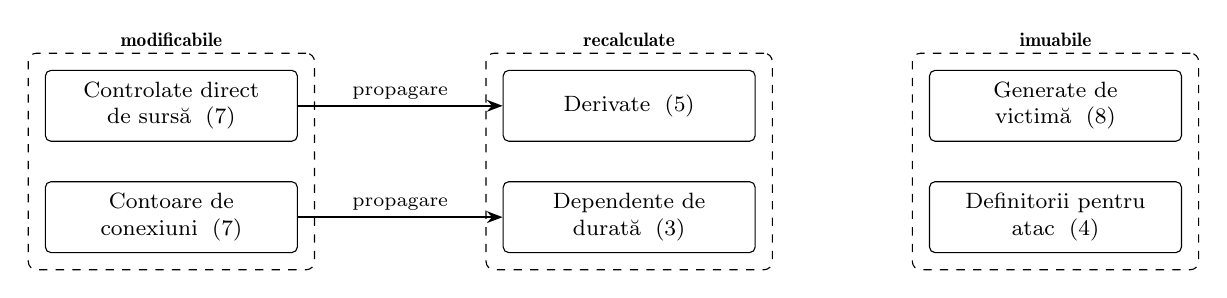
\begin{tikzpicture}[node distance=5mm and 8mm]
        \node[bloc, minimum width=32mm] (sursa) {Controlate direct\\ de sursă \;(7)};
        \node[bloc, minimum width=32mm, below=of sursa] (contoare) {Contoare de\\ conexiuni \;(7)};
        \node[bloc, minimum width=32mm, right=26mm of sursa] (derivate) {Derivate \;(5)};
        \node[bloc, minimum width=32mm, right=26mm of contoare] (cauzal) {Dependente de\\ durată \;(3)};
        \node[bloc, minimum width=32mm, right=22mm of derivate] (victima) {Generate de\\ victimă \;(8)};
        \node[bloc, minimum width=32mm, right=22mm of cauzal] (identitate) {Definitorii pentru\\ atac \;(4)};

        \draw[sageata] (sursa) -- node[eticheta, above] {propagare} (derivate);
        \draw[sageata] (contoare) -- node[eticheta, above] {propagare} (cauzal);

        \begin{scope}[on background layer]
            \node[grup, fit=(sursa)(contoare), label={[eticheta]above:\textbf{modificabile}}] {};
            \node[grup, fit=(derivate)(cauzal), label={[eticheta]above:\textbf{recalculate}}] {};
            \node[grup, fit=(victima)(identitate), label={[eticheta]above:\textbf{imuabile}}] {};
        \end{scope}
    \end{tikzpicture}
    \caption{Cele șase categorii care intervin în construcția perturbărilor, însumând 34 dintre cele 42 de caracteristici; restul de opt rămân în afara oricărei transformări și nu sunt reprezentate. Atacatorul acționează doar asupra grupului din stânga. Grupul din mijloc se modifică exclusiv prin propagare, iar cel din dreapta rămâne neschimbat.}
    \label{fig:taxonomie}
\end{figure}

Categoriile din tabelul~\ref{tab:taxonomie} se justifică după cum urmează.

\textbf{Caracteristicile controlate direct} sunt cele calculate exclusiv din pachetele emise de atacator: valoarea TTL a pachetelor trimise, volumul și numărul de pachete transmise, durata fluxului și parametrii ferestrei TCP. Modificarea lor corespunde unor acțiuni concrete la nivelul stivei de rețea a mașinii atacatoare.

\textbf{Contoarele de conexiuni} (denumite \textit{connection features} în documentația setului de date) numără câte dintre ultimele conexiuni înregistrate de senzor au aceeași sursă, aceeași destinație sau același serviciu ca fluxul analizat. Particularitatea lor este că nu descriu fluxul în sine, ci contextul în care acesta apare: două fluxuri identice în toate celelalte privințe primesc valori diferite dacă unul este izolat, iar celălalt face parte dintr-o serie de conexiuni către aceeași gazdă. Prefixul \verb|ct| din numele lor provine de la \textit{count}, iar sufixul \verb|ltm| de la \textit{last time}.

Ele sunt asimetrice din punctul de vedere al controlabilității: un atacator poate să le scadă, distribuind atacul în timp, dar nu le poate crește fără a genera trafic suplimentar, el însuși observabil. În consecință, perturbările asupra acestei categorii sunt admise doar în sens descrescător.

\textbf{Caracteristicile derivate} se calculează din altele și nu sunt niciodată stabilite direct de generator, ci recalculate în urma modificării mărimilor de bază, conform mecanismului din secțiunea~\ref{sec:consistenta}.

\textbf{Caracteristicile generate de victimă} (între care valoarea TTL a pachetelor de răspuns, volumul și numărul de pachete primite) nu pot fi stabilite de atacator. Ele constituie o rezervă de informație inaccesibilă, iar măsura în care un model se sprijină pe ea determină o limită naturală a evaziunii realizabile împotriva acelui model.

\textbf{Caracteristicile dependente de durată} reprezintă cazul intermediar discutat în subsecțiunea~\ref{subsec:directionalitate}. Ele sunt generate tot de victimă, dar nu sunt independente de acțiunea atacatorului: dacă acesta întârzie propriile pachete, răspunsurile victimei se întind și ele în timp, iar mărimile calculate din ele se modifică în consecință. Nu pot fi stabilite direct, ci doar prin propagare din raportul duratelor.

\textbf{Caracteristicile definitorii pentru atac} (protocolul, serviciul și starea conexiunii) sunt menținute constante, din motivele expuse în subsecțiunea~\ref{subsec:stare}.

\subsection{Accesul atacatorului la sistemul de detecție}\label{subsec:acces}

Se presupune că atacatorul nu dispune de parametrii modelului, de informația de gradient, de scorurile de încredere asociate predicțiilor și nici de o interfață prin care să poată interoga modelul, fie și numai pentru a obține eticheta prezisă. Perturbările sunt construite exclusiv pe baza proprietăților statistice observabile ale traficului, adică pe baza cunoașterii modului în care arată traficul legitim într-o rețea, nu pe baza vreunei reacții a sistemului de detecție.

Această ipoteză este cea mai restrictivă dintre variantele uzuale și, din acest motiv, produce estimări conservatoare: un atacator cu acces suplimentar ar obține rezultate cel puțin la fel de bune. Alegerea corespunde situației practice în care sistemul de detecție se află în infrastructura apărătorului și nu expune niciun canal de răspuns către exterior.

Ipoteza are însă și o consecință metodologică ce depășește realismul scenariului. Întrucât perturbarea nu depinde în niciun fel de model, exact aceleași variante perturbate pot fi aplicate tuturor modelelor evaluate. Comparația dintre modele devine astfel un experiment controlat: intrarea este identică, iar singura mărime care variază este modelul însuși. Orice diferență observată între ratele de evaziune este atribuibilă modelului, nu unei diferențe între perturbările la care a fost supus. Dacă perturbările ar fi fost optimizate separat pentru fiecare model, această atribuire nu ar mai fi fost posibilă.

Metodele care exploatează informația de gradient, precum FGSM \cite{goodfellow2015explaining}, se situează în afara acestui model de amenințare. Ele presupun accesul la derivatele funcției de decizie și, suplimentar, sunt aplicabile doar modelelor diferențiabile, ceea ce exclude ansamblurile de arbori. Chiar și atunci când sunt aplicabile, aceste metode produc perturbări direct în spațiul valorilor numerice, fără garanția că rezultatul corespunde unui trafic realizabil \cite{zhang2022adversarial, he2023adversarial}. Excluderea lor nu este, prin urmare, o afirmație despre inaplicabilitatea lor generală, ci o delimitare a cadrului adoptat aici.

\subsection{Mulțimea perturbărilor admisibile}\label{subsec:admisibile}

Reunind elementele anterioare, mulțimea perturbărilor admisibile se definește prin patru condiții simultane.

\begin{enumerate}
    \item \textbf{Direcționalitate.} Fiecare tip de transformare acționează într-un singur sens, determinat de acțiunea fizică pe care o reprezintă: volumul transmis poate doar să crească, durata poate doar să crească, contoarele de conexiuni pot doar să scadă.
    \item \textbf{Limite de domeniu relative.} Valorile rezultate trebuie să rămână în limitele fizic realizabile ale protocolului. Aceste limite se aplică relativ la valorile fluxului original, nu ca praguri absolute stabilite teoretic, deoarece capturile reale conțin ele însele înregistrări care încalcă limitele nominale. Impunerea unor praguri absolute ar respinge fluxuri care există efectiv în date.
    \item \textbf{Imuabilitate.} Caracteristicile generate de victimă și cele definitorii pentru identitatea atacului rămân neschimbate.
    \item \textbf{Închidere la dependențe.} Orice modificare a unei caracteristici de bază este însoțită de recalcularea tuturor caracteristicilor derivate din ea, astfel încât varianta rezultată să fie intern consistentă.
\end{enumerate}

Condiția a patra ridică cele mai multe dificultăți și face obiectul secțiunii următoare.

\section{Consistența internă a vectorului de caracteristici}\label{sec:consistenta}

\subsection{Problema inconsistenței induse}\label{subsec:inconsistenta}

Se consideră o perturbare care crește volumul de octeți transmiși prin adăugarea de umplutură în conținutul pachetelor. Dacă se modifică doar mărimea corespunzătoare, restul rezumatului rămâne cel calculat pentru volumul inițial. Rezultatul descrie un flux în care volumul transmis a crescut, dar dimensiunea medie a pachetului și debitul au rămas neschimbate, o combinație pe care niciun senzor de rețea nu ar putea să o producă, întrucât cele trei mărimi sunt legate prin relații deterministe.

Consecința asupra măsurătorii este severă. Dacă modelul își schimbă decizia pentru un asemenea flux, nu se poate stabili dacă a reacționat la perturbarea intenționată sau la imposibilitatea aritmetică a intrării. În al doilea caz, rata de evaziune măsurată nu ar caracteriza robustețea modelului la trafic modificat, ci comportamentul lui pe intrări situate în afara oricărei distribuții realiste. Consistența internă este deci o condiție de validitate a întregului experiment.

\subsection{Propagarea prin rapoarte}\label{subsec:propagare}

Soluția directă ar fi recalcularea caracteristicilor derivate din formulele documentate ale senzorului. Această abordare se lovește însă de o dificultate practică: formulele documentate nu reproduc exact valorile stocate în setul de date, întrucât constantele de conversie și convențiile de rotunjire folosite de senzor nu sunt pe deplin specificate. Recalcularea ar înlocui valoarea originală cu una ușor diferită, introducând o abatere în toate fluxurile, inclusiv în cele neperturbate, ceea ce ar încălca invariantul identității.

Se adoptă, în schimb, o abordare bazată pe rapoarte, justificată de următoarea observație.

\medskip
\noindent\textbf{Observația centrală.} \textit{Fie o caracteristică derivată care se obține împărțind o mărime de bază la alta și înmulțind rezultatul cu o constantă necunoscută, dar aceeași pentru toate fluxurile. Dacă perturbarea modifică mărimile de bază, atunci valoarea nouă a caracteristicii derivate se obține luând valoarea ei originală, înmulțind-o cu raportul dintre valoarea nouă și cea veche a mărimii de la numărător și împărțind-o la raportul corespunzător al mărimii de la numitor. Rezultatul este exact, indiferent de valoarea constantei necunoscute.}

\medskip

Constanta necunoscută intervine în același fel atât în valoarea originală, cât și în cea nouă. Atunci când valoarea nouă este exprimată prin cea veche, constanta apare o dată la numărător și o dată la numitor, deci se simplifică. Nu este nevoie, prin urmare, ca ea să fie determinată.

Această proprietate are două consecințe practice. Prima este că nu este necesară reconstituirea prin inginerie inversă a convențiilor senzorului: relațiile pot fi propagate corect fără a le cunoaște constantele. A doua, mai importantă, este că valoarea originală apare ca factor în rezultat. Pentru o perturbare nulă, ambele rapoarte devin egale cu unitatea, iar procedura redă exact valoarea stocată inițial, nu o aproximare a ei. Se păstrează astfel invariantul identității, care ar fi fost încălcat de recalcularea din formulă.

Modul în care se propagă modificările este prezentat în tabelul~\ref{tab:propagare}.

\begin{table}[!ht]
    \caption{Modul în care se propagă modificările asupra caracteristicilor derivate}
    \centering
    \begin{tabular}{|l|p{7.2cm}|}
        \hline
        \textbf{Caracteristică derivată} & \textbf{Cum se modifică} \\
        \hline
        Dimensiunea medie a pachetului & Crește proporțional cu volumul transmis și scade proporțional cu numărul de pachete \\
        \hline
        Debitul sursei & Crește proporțional cu volumul transmis și scade proporțional cu durata \\
        \hline
        Rata globală de pachete & Crește proporțional cu numărul total de pachete și scade proporțional cu durata \\
        \hline
        Intervalul mediu dintre pachete & Crește proporțional cu durata și scade proporțional cu numărul de intervale dintre pachete \\
        \hline
        Fluctuația temporală & Se modifică proporțional cu durata \\
        \hline
        Debitul destinației & Scade proporțional cu durata, volumul primit rămânând neschimbat \\
        \hline
    \end{tabular}
    \label{tab:propagare}
\end{table}

Cazurile degenerate necesită tratament explicit. Dacă o mărime de bază are valoarea zero în fluxul original, raportul corespunzător nu poate fi calculat, iar modificarea nu poate fi propagată. Situația apare pentru fluxurile formate dintr-un singur pachet, pentru care numărul de intervale dintre pachete este nul, și pentru cele cu durată înregistrată zero. În aceste cazuri caracteristica derivată se lasă neschimbată. Alegerea este conservatoare: ea reduce amplitudinea perturbării efective, deci nu poate produce o supraestimare a evaziunii.

\subsection{Caracteristici nereconstituibile și rezultate sub formă de interval}\label{subsec:interval}

Nu toate caracteristicile derivate se supun regulii de mai sus. Un caz distinct îl constituie contorul care combină starea conexiunii cu valorile TTL observate, numit în continuare \emph{contorul de context}, întrucât valoarea lui descrie situația în care apare fluxul, nu fluxul însuși. Analiza datelor arată că acest contor nu este o funcție a valorilor TTL ale fluxului curent: există perechi de fluxuri cu valori TTL apropiate cărora le corespund valori diferite ale contorului, precum și perechi cu valori TTL foarte diferite cărora le corespunde aceeași valoare. Comportamentul este consistent cu definiția sa reală, aceea de contor calculat pe o fereastră glisantă peste conexiunile recente.

Rezultă că mărimea nu poate fi calculată pornind de la un flux izolat: ea depinde de contextul în care fluxul apare, iar acest context nu este disponibil în reprezentarea tabelară. În consecință, valoarea pe care senzorul ar calcula-o pentru un flux perturbat nu poate fi determinată din datele existente.

Această nedeterminare nu poate fi eliminată, dar poate fi delimitată. Se definesc două politici explicite, corespunzătoare unor ipoteze extreme privind comportamentul contorului:

\begin{description}[style=nextline]
    \item[Politica conservatoare.] Contorul rămâne la valoarea din fluxul original. Ea corespunde ipotezei că modificarea TTL nu influențează contextul agregat, ceea ce subestimează efectul perturbării.
    \item[Politica optimistă.] Contorul adoptă valoarea tipică traficului legitim având aceeași valoare TTL. Ea corespunde ipotezei că atacatorul reușește să reproducă integral semnătura de context a traficului normal, ceea ce supraestimează efectul perturbării.
\end{description}

Evaluând rata de evaziune sub ambele politici se obține un interval, raportat ca atare în locul unei valori unice.

Natura acestui interval trebuie precizată, pentru a evita o interpretare greșită. El nu exprimă incertitudine statistică și nu are semnificația unui interval de încredere: nu provine din variabilitatea de eșantionare și nu i se poate asocia un nivel de acoperire. El reprezintă amplitudinea rezultatului între două ipoteze explicit formulate privind o mărime care nu poate fi reconstituită din date. Lățimea intervalului este ea însăși informativă: un interval îngust arată că rezultatul nu depinde practic de ipoteza adoptată, în timp ce un interval larg semnalează că o parte substanțială a efectului măsurat este condiționată de o presupunere care nu poate fi verificată.

Aceeași logică a delimitării explicite se aplică și caracteristicilor aflate în afara controlului atacatorului. Pe lângă perturbările realizabile, se poate evalua un scenariu de referință cu constrângeri relaxate, în care se modifică și caracteristicile generate de victimă. Un asemenea scenariu nu descrie un atac practic și nu poate fi raportat alături de rezultatele realizabile, rolul său este strict de a cuantifica ce parte din dependența unui model de o familie de caracteristici se sprijină pe informație inaccesibilă atacatorului.

\section{Algoritmii propuși}\label{sec:algoritmi}

Principiile prezentate anterior sunt puse în practică în patru proceduri, descrise independent de detaliile de implementare. Succesiunea etapelor urmărește respectarea constrângerilor definite în secțiunile precedente.

\subsection{Generarea unei variante perturbate}\label{subsec:alg-generare}

Procedura primește un flux și o transformare și produce fie o variantă validă, fie un refuz. Ordinea pașilor nu este arbitrară: propagarea trebuie să urmeze modificării de bază, iar validarea trebuie să fie ultima, altfel ar verifica o stare intermediară.

\begin{algorithm}[!ht]
\caption{Generarea unei variante perturbate}\label{alg:generare}
\begin{enumerate}\itemsep2pt
    \item Se pornește de la fluxul original și de la tipul și intensitatea transformării.
    \item Se stabilesc caracteristicile de bază vizate de transformare: valoarea TTL, volumul transmis, durata sau contoarele de conexiuni, respectând sensul unic admis pentru fiecare.
    \item Dacă transformarea a modificat volumul, se verifică limita de dimensiune a pachetului; la depășire, se adaugă pachete în loc să fie încălcată limita.
    \item Se recalculează toate caracteristicile derivate din cele modificate, prin procedura din subsecțiunea~\ref{subsec:alg-propagare}.
    \item Dacă valoarea TTL s-a schimbat, se stabilește și contorul de context. Acesta nu poate fi calculat din fluxul izolat, deci nu se recalculează, ci se alege conform uneia dintre cele două politici definite în subsecțiunea~\ref{subsec:interval}. Politica folosită se consemnează împreună cu varianta, întrucât de ea depinde marginea de interval pe care o va produce măsurarea.
    \item Se verifică cele șase condiții de validitate. Dacă vreuna este încălcată, varianta este \textbf{respinsă}, nu corectată.
    \item Se returnează varianta împreună cu evidența modificărilor efectuate.
\end{enumerate}
\end{algorithm}

Pasul 6 merită subliniat: o variantă care încalcă o constrângere nu este ajustată tacit până devine acceptabilă, ci semnalată ca eroare. Corectarea automată ar produce o variantă diferită de cea cerută, iar rezultatul măsurat nu ar mai corespunde parametrilor raportați.

\subsection{Propagarea caracteristicilor derivate}\label{subsec:alg-propagare}

Procedura pune în aplicare observația centrală din subsecțiunea~\ref{subsec:propagare}. Ea nu recalculează caracteristicile derivate din formulele senzorului, ci le modifică proporțional cu rapoartele dintre valorile noi și cele vechi ale mărimilor din care provin.

\begin{algorithm}[!ht]
\caption{Propagarea prin rapoarte}\label{alg:propagare}
\begin{enumerate}\itemsep2pt
    \item Pentru fiecare mărime de bază modificată se calculează raportul dintre valoarea nouă și cea originală.
    \item Dacă valoarea originală este nulă, raportul nu poate fi calculat; caracteristica derivată se lasă neschimbată.
    \item Fiecare caracteristică derivată se modifică proporțional cu rapoartele mărimilor din care se calculează, direct sau invers, după cum acestea apar la numărător sau la numitor.
    \item Mărimile temporale ale traficului de retur se modifică exclusiv cu raportul duratelor, conform discuției din subsecțiunea~\ref{subsec:directionalitate}.
    \item Se raportează numărul de fluxuri pentru care propagarea a fost neutralizată la pasul 2.
\end{enumerate}
\end{algorithm}

Pasul 5 permite identificarea situațiilor în care propagarea nu produce modificările așteptate. Dacă acest lucru se întâmplă pentru un număr mare de fluxuri, intensitatea efectivă a perturbării este mai redusă decât cea stabilită, iar efectul său poate fi subestimat.

\subsection{Măsurarea ratei de evaziune}\label{subsec:alg-masurare}

\begin{algorithm}[H]
\caption{Măsurarea ratei de evaziune}\label{alg:masurare}
\begin{enumerate}\itemsep2pt
    \item Se calculează predicțiile modelului pe traficul nemodificat și se determină fluxurile asupra cărora se face măsurarea, conform criteriului din subsecțiunea~\ref{subsec:eligibil}.
    \item Se verifică invariantul identității. Dacă rata obținută pe perturbarea nulă nu este exact zero, procedura se oprește: lanțul de măsurare este defect.
    \item Pentru fiecare transformare și fiecare nivel de intensitate se generează varianta corespunzătoare prin Algoritmul~\ref{alg:generare}.
    \item Se calculează predicțiile pe varianta perturbată, restrânse la fluxurile stabilite la pasul 1.
    \item Fiecare flux se încadrează în unul dintre cele trei rezultate din subsecțiunea~\ref{subsec:rezultate}, iar rata de evaziune se obține ca proporție a cazurilor de tipul (b).
    \item Pentru transformările cu două politici de context, cele două rate obținute delimitează intervalul discutat în subsecțiunea~\ref{subsec:interval}.
\end{enumerate}
\end{algorithm}

Pasul 2 este plasat înaintea evaluării, nu după ea, pentru că verifică însăși funcționarea procedurii. Perturbarea nulă nu modifică niciun flux, așa că o rată de evaziune nenulă în acest punct nu poate veni din perturbare, ci doar dintr-o defecțiune a lanțului de măsurare. Lăsată la final, aceeași verificare ar scoate defecțiunea la iveală abia după parcurgerea întregii grile, când rezultatele produse între timp ar fi consistente între ele și greu de deosebit de unele corecte.


\subsection{Analiza sensibilității}\label{subsec:alg-sensibilitate}

\begin{algorithm}[!ht]
\caption{Determinarea importanței și corelarea cu evaziunea}\label{alg:sensibilitate}
\begin{enumerate}\itemsep2pt
    \item Se măsoară proporția fluxurilor de atac pe care modelul le semnalează, pe date nemodificate.
    \item Pentru fiecare caracteristică, valorile ei se înlocuiesc cu valori extrase dintr-o distribuție exterioară, astfel încât legătura dintre caracteristică și etichetă să fie ruptă efectiv.
    \item Se remăsoară proporția de la pasul 1; scăderea observată constituie importanța caracteristicii. Substituția se repetă de mai multe ori, iar rezultatele se mediază.
    \item Se însumează importanțele pe categoriile de controlabilitate din tabelul~\ref{tab:taxonomie}, obținând proporția din capacitatea de detecție aflată la îndemâna atacatorului.
    \item Pentru fiecare transformare se însumează importanțele caracteristicilor pe care le afectează, iar seria rezultată se corelează cu ratele de evaziune măsurate.
\end{enumerate}
\end{algorithm}

Pasul 2 ascunde o subtilitate care s-a dovedit necesară în practică. Modul obișnuit de a rupe legătura dintre o caracteristică și etichetă este amestecarea valorilor ei în interiorul eșantionului analizat. Procedeul funcționează cât timp eșantionul este divers, dar se golește de conținut atunci când analiza se restrânge la o singură clasă de atac: dacă acolo caracteristica ia aproape aceeași valoare pentru toate observațiile, amestecarea le schimbă între ele fără să schimbe nimic, iar importanța rezultată apare nulă tocmai pentru o caracteristică pe care modelul se poate sprijini decisiv. Extragerea valorilor de înlocuire dintr-o distribuție exterioară eșantionului elimină acest artefact.

\section{Fundamentarea alegerii modelelor de clasificare}\label{sec:alegerea-modelelor}

Lucrarea compară trei modele: două ansambluri de arbori de decizie și o arhitectură neuronală bazată pe atenție. Alegerea nu urmărește acoperirea unui spectru cât mai larg de algoritmi, ci contrastarea a două familii cu moduri fundamental diferite de a construi decizia, întrucât tocmai această diferență este cea susceptibilă să se reflecte în comportamentul sub perturbări.

\subsection{Ansambluri de arbori de decizie}\label{subsec:arbori}

Ambele modele din prima familie construiesc decizia prin împărțiri succesive ale spațiului caracteristicilor, fiecare împărțire comparând o singură caracteristică cu un prag. Cele două sunt denumite în continuare prin numele lor consacrate, \textit{Random Forest} și \textit{XGBoost}. Denumirile descriptive, pădure aleatoare și creștere prin gradient, ar acoperi întreaga familie de algoritmi, nu implementările concrete ale căror rezultate sunt raportate aici.

\textbf{Random Forest} \cite{breiman2001random} combină predicțiile a sute de arbori, fiecare antrenat pe un eșantion diferit al datelor și fiecare alegându-și pragurile dintr-un subset de caracteristici extras aleator la fiecare nod. Cele două surse de aleatoriu îi fac pe arbori să greșească în locuri diferite, iar media predicțiilor anulează o parte dintre aceste erori fără să deplaseze decizia de ansamblu. Selecția aleatoare a caracteristicilor are și un efect care privește direct tema lucrării: fiindcă la fiecare nod doar o parte dintre caracteristici sunt disponibile, arborii nu ajung să se sprijine toți pe aceeași mărime dominantă, iar capacitatea de detecție se distribuie peste mai multe caracteristici.

\textbf{XGBoost} \cite{chen2016xgboost} construiește ansamblul secvențial, fiecare arbore nou fiind ajustat pe erorile rămase de la cei anteriori, prin optimizarea unei funcții obiectiv care include și un termen de regularizare. Spre deosebire de agregarea prin mediere, procedura reduce eroarea sistematică și tinde să exploateze intensiv caracteristicile cu putere predictivă ridicată. Din perspectiva teoretică a lucrării, aceasta conduce la o predicție verificabilă experimental: concentrarea capacității de detecție într-un număr mic de caracteristici ar trebui să crească vulnerabilitatea la o perturbare care vizează exact acele caracteristici.

Ambele modele au o proprietate comună cu consecințe metodologice directe: împărțirea spațiului folosește doar ordinea valorilor unei caracteristici, nu și magnitudinea acestora. Modelele sunt, prin urmare, insensibile la orice transformare care păstrează ordinea valorilor, iar aducerea numerelor la o scară comună nu le modifică deciziile. Aceeași proprietate explică însă și de ce o singură caracteristică poate domina decizia: un prag pe o caracteristică puternic corelată cu eticheta separă eficient clasele fără a necesita nicio combinație cu altele, iar mecanismul de construcție îl va prefera sistematic.

\subsection{Arhitectura bazată pe atenție pentru date tabelare}\label{subsec:atentie}

Arhitectura de tip transformer \cite{vaswani2017attention} a fost concepută pentru date secvențiale, precum textul, și nu se aplică direct datelor tabelare: nu există o secvență peste care să fie calculată atenția, iar ordinea coloanelor este arbitrară. Adaptarea folosită în lucrare urmează abordarea propusă de Gorishniy et al. \cite{gorishniy2021revisiting}, în care fiecare caracteristică este transformată într-un vector, iar mulțimea vectorilor astfel obținuți joacă rolul secvenței.

Concret, fiecare coloană numerică este transformată într-un vector printr-o operație liniară proprie, cu parametri învățați în timpul antrenării, iar fiecare coloană categorică primește un tabel de vectori indexat după valoarea categoriei. La secvența astfel obținută se adaugă un vector suplimentar, cu rol de agregator, din reprezentarea căruia se face în final clasificarea.

Peste această secvență se aplică blocuri succesive de auto-atenție. Mecanismul funcționează astfel: pentru fiecare pereche de elemente ale secvenței se calculează o măsură de asemănare, iar aceste măsuri sunt apoi normalizate, astfel încât ponderile asociate unui element să însumeze unitatea. În final, fiecare element este recalculat ca o combinație a tuturor celorlalte, ponderată cu valorile obținute. Operația se execută în paralel de mai multe ori, cu seturi diferite de parametri, ceea ce permite modelului să urmărească simultan mai multe tipuri de relații între caracteristici.

Diferența de mod de lucru față de ansamblurile de arbori este esențială pentru comparație. Mecanismul de atenție calculează ponderi pentru fiecare pereche de caracteristici, deci modelul reprezintă explicit relații între câte două mărimi, într-o formă continuă și învățată. Un ansamblu de arbori poate reprezenta asemenea relații doar implicit, prin înlănțuirea pragurilor pe ramuri succesive.

Această diferență atrage și o consecință metodologică. Spre deosebire de arbori, o rețea neuronală nu este insensibilă la scara valorilor: caracteristicile cu domenii de ordine de mărime diferite ar contribui disproporționat la ajustarea parametrilor. Modelul bazat pe atenție necesită, prin urmare, aducerea valorilor numerice la o scară comună, în timp ce ansamblurile de arbori nu o necesită. Este important de subliniat că această diferență de pregătire a datelor nu afectează validitatea comparației: mulțimea caracteristicilor, împărțirea în seturi de antrenare și testare și etichetele rămân identice pentru toate modelele. Aducerea la scară comună este o etapă internă unui singur model, nu o modificare a datelor comparate.

\subsection{Ce izolează comparația}\label{subsec:comparatie}

O comparație între modele spune ceva despre modele numai dacă tot restul rămâne neschimbat. Aici sunt ținute fixe patru lucruri: datele și împărțirea lor în seturi, mulțimea caracteristicilor, criteriul după care se aleg fluxurile pe care se măsoară și, pentru că perturbările nu depind în niciun fel de model, conform subsecțiunii~\ref{subsec:acces}, chiar variantele perturbate, identice rând cu rând pentru toate cele trei modele. Singura mărime care variază rămâne astfel modelul însuși, iar o diferență între ratele de evaziune se poate atribui felului în care fiecare își construiește decizia.

Comparația face însă și o distincție mai fină. Dacă un model cedează mai puțin decât celelalte, explicația poate fi una dintre două, iar ratele singure nu le deosebesc: fie modelul a învățat o reprezentare care nu se sprijină pe proprietăți ușor de modificat, fie se sprijină preponderent pe caracteristici la care atacatorul oricum nu ajunge. Prima ar fi o proprietate a arhitecturii, transferabilă la alte date, a doua, o consecință a felului în care au fost generate tocmai aceste date. Concluziile practice sunt opuse, iar separarea lor cere analiza de sensibilitate din secțiunea~\ref{sec:sensibilitate}.

\section{Evaluarea în condiții de dezechilibru sever}\label{sec:metrici}

Seturile de date pentru detecția intruziunilor sunt caracterizate de un dezechilibru pronunțat între clase \cite{ring2019survey, moustafa2015unsw}: categoriile de atac rare pot fi de câteva sute de ori mai puțin frecvente decât traficul normal. Alegerea metricilor de evaluare trebuie să țină cont de această situație.

Acuratețea globală, definită ca proporția predicțiilor corecte din total, este inadecvată. Într-un set în care o clasă acoperă o fracțiune majoritară din observații, un clasificator degenerat care prezice constant acea clasă obține o valoare ridicată fără a avea vreo capacitate de discriminare. Valoarea metricii este dominată de clasele frecvente, iar comportamentul pe clasele rare, chiar cele care corespund atacurilor mai puțin obișnuite devine practic invizibil.

Se folosesc, în consecință, metrici care acordă pondere egală fiecărei clase. Pentru fiecare categorie în parte se calculează trei mărimi. \emph{Precizia} arată ce proporție dintre fluxurile pe care modelul le-a atribuit acelei categorii îi aparțin în realitate, adică măsoară cât de multe alarme false produce modelul pentru categoria respectivă. \emph{Sensibilitatea} arată ce proporție dintre fluxurile care aparțin în realitate categoriei au fost efectiv recunoscute, adică măsoară cât de multe scapă nedetectate. \emph{Scorul F1} le combină pe amândouă într-o singură valoare, construită astfel încât să fie mică ori de câte ori una dintre cele două este mică, un model nu poate obține un scor bun sacrificând-o pe una în favoarea celeilalte.

Performanța globală se rezumă apoi prin media neponderată a scorurilor F1 ale tuturor categoriilor. Faptul că media este neponderată este esențial: el face ca eșecul pe o clasă rară să conteze exact la fel de mult ca eșecul pe una frecventă. Se raportează suplimentar media sensibilităților per clasă, precum și matricea de confuzie, care este singura reprezentare ce arată nu doar cât de des greșește modelul, ci și \emph{unde} plasează erorile, informație necesară pentru interpretarea rezultatului de tip (c).

Dezechilibrul este tratat și în etapa de antrenare, prin acordarea unei ponderi mai mari observațiilor din clasele rare, invers proporțională cu frecvența lor. În absența acestei corecții, contribuția claselor rare la mărimea pe care o optimizează procedura de antrenare devine neglijabilă, iar acestea ajung să fie ignorate.

O ultimă observație leagă această secțiune de criteriul din subsecțiunea~\ref{subsec:eligibil}. Un scor mediu moderat nu implică o capacitate slabă de semnalare a atacurilor. Cele două mărimi măsoară lucruri diferite: media penalizează încadrarea greșită a unui atac într-o categorie vecină, în timp ce semnalarea alarmei rămâne corectă în acel caz. Este perfect posibil ca un model să confunde frecvent categorii de atac apropiate ca profil, păstrând totodată o capacitate aproape completă de a distinge traficul malițios de cel legitim. Această observație justifică definirea mulțimii de măsurare pe criteriul semnalării, și nu pe cel al clasificării corecte: dacă cele două ar coincide, alegerea numitorului ar fi lipsită de consecințe.

\section{Fundamentarea analizei de sensibilitate}\label{sec:sensibilitate}

Măsurarea ratei de evaziune arată \emph{cât} cedează un model, dar nu explică \emph{de ce}. Explicația necesită o măsură a dependenței modelului de fiecare caracteristică, comparabilă între cele trei modele și exprimată în aceleași unități ca evaziunea.

\subsection{Necesitatea unei măsuri independente de model}\label{subsec:agnostic}

Fiecare dintre cele trei modele își raportează importanța altfel: Random Forest prin reducerea de impuritate, XGBoost prin câștigul acumulat în punctele de separare, iar modelul de tip Transformer prin ponderile mecanismului de atenție. Nu diferă doar formulele, ci și unitățile în care sunt exprimate, așa că valorile nu se pot pune una lângă alta. Cum aici se compară tocmai modelele între ele, e nevoie de o măsură unică, obținută în același fel pentru toate trei.

Importanța prin permutare este o astfel de măsură. Ea pornește de la o singură întrebare: ce se schimbă dacă o caracteristică nu mai spune nimic despre flux? Un model care se sprijinea pe ea ar trebui să înceapă să greșească vizibil, iar unul care nu o folosea ar trebui să nu simtă diferența. Se înlocuiesc, așadar, valorile acelei caracteristici cu valori străine de fluxul analizat, restul rezumatului rămâne neatins, iar cât pierde modelul din performanță devine chiar importanța caracteristicii. Nimic din procedură nu presupune ceva despre interiorul modelului și nimic nu cere reantrenare, deci cele trei modele înghețate pot fi trecute prin exact același test.

\subsection{Alegerea metricii și comparabilitatea}\label{subsec:comensurabil}

Alegerea mărimii a cărei degradare se măsoară este esențială. Se adoptă \emph{proporția fluxurilor malițioase încă semnalate ca atare}. Motivul este că această mărime este exact complementara celei măsurate prin rata de evaziune: evaziunea înseamnă că un flux de atac încetează să mai fie semnalat, iar scăderea proporției respective măsoară exact același fenomen.

În consecință, afirmațiile „modelul se sprijină în cutare măsură pe caracteristica X” și „perturbarea caracteristicii X produce o evaziune de cutare procent” sunt exprimate în aceleași unități și pot fi puse în corespondență direct, prin corelarea celor două serii de valori, nu doar prin analogie calitativă. Dacă mărimea aleasă ar fi fost, de exemplu, media scorurilor F1, cele două ar fi rămas legate doar intuitiv.

\subsection{Importanța accesibilă atacatorului}\label{subsec:accesibila}

Combinând măsura de mai sus cu partiționarea din tabelul~\ref{tab:taxonomie} se obține mărimea care leagă întreaga construcție teoretică. Se însumează importanțele tuturor caracteristicilor pe care atacatorul le poate modifica și se raportează rezultatul la suma importanțelor tuturor caracteristicilor. Se obține astfel o proporție, cuprinsă între zero și unu, numită în continuare \emph{fracțiunea accesibilă} a capacității de detecție. Importanțele negative, care apar atunci când amestecarea unei caracteristici îmbunătățește întâmplător rata de detecție, sunt trunchiate la zero înaintea însumării, atât la numărător, cât și la numitor. Fără această convenție, o sumă cu termeni de semne opuse ar putea produce proporții în afara intervalului sau instabile la variații mici ale măsurătorii.

Mărimea admite o interpretare directă: ea arată ce parte din informația pe care modelul o folosește efectiv pentru a semnala atacurile se află la îndemâna unui atacator. Un model cu o fracțiune accesibilă mică își sprijină decizia preponderent pe informație pe care atacatorul nu o poate atinge, ceea ce limitează evaziunea realizabilă independent de calitatea reprezentării învățate. Distincția introdusă în subsecțiunea~\ref{subsec:comparatie}, între rezistența datorată reprezentării și cea datorată inaccesibilității, devine astfel măsurabilă, iar nu doar enunțabilă.

\subsection{Limita atribuirii pe o singură caracteristică}\label{subsec:limita}

Procedura descrisă înlocuiește o singură caracteristică pe rând și, prin construcție, nu poate detecta efectele care apar doar la modificarea simultană și coerentă a mai multor caracteristici legate între ele. Dacă decizia modelului depinde de o combinație de valori, iar nu de fiecare valoare în parte, înlocuirea izolată a oricăreia dintre ele va produce o degradare modestă, sugerând în mod eronat o dependență redusă.

Această limitare are o consecință importantă pentru interpretarea rezultatelor: importanța atribuită individual constituie o limită inferioară a vulnerabilității adversariale, nu o estimare a ei. Ea justifică totodată, din nou, cerința de închidere la dependențe formulată în subsecțiunea~\ref{subsec:admisibile}: o metodologie care ar perturba caracteristicile izolat, fără propagare, ar rata tocmai efectele de acest tip.

\section{Antrenarea adversarială ca problemă de proiectare experimentală}\label{sec:antrenare}

Secțiunile anterioare au construit aparatul necesar pentru a măsura cât de ușor poate fi ocolit un sistem de detecție. Întrebarea complementară este dacă vulnerabilitatea astfel identificată poate fi redusă prin însuși modul în care modelul este antrenat. Ideea este simplă și veche: dacă modelul vede, în timpul antrenării, nu doar fluxurile de atac originale, ci și variante modificate ale acestora, etichetate în continuare drept malițioase, atunci este împins să recunoască atacul după proprietățile care rămân neschimbate sub transformare, nu după cele care se pot schimba.

Dificultatea nu stă în aplicarea ideii, ci în măsurarea corectă a efectului ei. Această secțiune arată de ce comparația directă dintre modelul reantrenat și cel inițial nu este suficientă și ce anume trebuie ținut fix pentru ca îmbunătățirea observată să poată fi atribuită perturbării.

\subsection{De ce augmentare și nu generare prin gradient}\label{subsec:de-ce-augmentare}

Există două moduri de a obține exemplele adăugate. În primul, ele sunt construite folosind derivatele funcției de decizie a modelului aflat în curs de antrenare, deci urmăresc granița de decizie pe măsură ce aceasta se deplasează. În al doilea, ele provin dintr-un set de transformări definite în prealabil, aplicate independent de reacția modelului.

Pentru cadrul construit aici, doar a doua variantă este disponibilă, din trei motive care se cumulează. Primul ține de simetria cu partea de atac: perturbările evaluate în subsecțiunea~\ref{subsec:lp} sunt construite fără acces la parametrii sau la răspunsurile modelului, iar o apărare antrenată pe exemple obținute prin gradient ar fi confruntată cu un atacator care nu dispune de aceeași informație. Comparația ar amesteca atunci două lucruri distincte, puterea metodei de generare și accesul presupus al atacatorului. Al doilea motiv ține de modelele analizate: ansamblurile de arbori nu admit derivate ale funcției de decizie în raport cu intrările, deci pentru două dintre cele trei clasificatoare metoda nu poate fi aplicată deloc, iar o apărare disponibilă doar pentru unul dintre ele nu ar permite compararea celor trei în aceleași condiții. Al treilea motiv, și cel mai important, este cel de realizabilitate: un exemplu obținut prin deplasarea vectorului de caracteristici în direcția indicată de derivate nu corespunde în mod necesar unui flux care poate fi generat efectiv, iar antrenarea pe astfel de exemple ar învăța modelul să reziste unor intrări care nu pot să apară în realitate.

Exemplele adăugate sunt, prin urmare, produse de același mecanism care generează variantele folosite la măsurarea evaziunii, cu aceleași verificări de admisibilitate și aceeași propagare a caracteristicilor derivate. Apărarea și atacul rămân astfel definite în raport cu aceeași mulțime de transformări, ceea ce face ca rezultatul să fie interpretabil: se măsoară rezistența la exact familia de modificări pentru care s-a demonstrat anterior vulnerabilitatea, nu la o familie mai largă și nici la una mai îngustă.

\subsection{Ce se schimbă simultan atunci când se adaugă exemple perturbate}\label{subsec:confuzii}

Copiile perturbate se adaugă fluxurilor originale, care rămân în setul de antrenare. Această alegere are o consecință care trebuie enunțată explicit, pentru că determină întreaga construcție experimentală: adăugarea unor copii doar pentru fluxurile de atac modifică simultan trei lucruri, nu unul singur.

Se modifică, în primul rând, cantitatea de exemple malițioase disponibile la antrenare. Un model antrenat pe mai multe exemple de atac poate detecta mai bine atacurile pentru simplul motiv că a văzut mai multe, independent de faptul că exemplele adăugate sunt sau nu perturbate. În al doilea rând, se modifică proporția dintre traficul normal și cel malițios. Într-un cadru dezechilibrat, această proporție influențează direct poziția granițelor de decizie, deci un efect apare chiar și în absența oricărei perturbări. În al treilea rând, dacă modelul folosește ponderi de clasă derivate din frecvențele observate, acestea se recalculează pe numărătorile modificate, deci se schimbă și funcția de cost minimizată, nu doar datele pe care este minimizată.

Un rezultat obținut prin compararea modelului reantrenat cu cel inițial nu poate distinge între aceste trei efecte și cel al perturbării propriu-zise. O scădere a ratei de evaziune ar fi observată și dacă exemplele adăugate ar fi simple copii ale celor existente, iar atribuirea ei perturbării ar fi nejustificată.

\subsection{Grupul de control și ce anume izolează}\label{subsec:control}

Soluția constă în adăugarea unui al treilea model, antrenat pe un set construit astfel încât să difere de cel al modelului apărat printr-o singură proprietate. Acest grup de control primește exact același număr de exemple de atac suplimentare, provenite din exact aceleași fluxuri sursă, dar neperturbate: simple duplicate ale înregistrărilor originale.

Prin construcție, cele două seturi au același număr de rânduri, aceeași distribuție a claselor și același efort de antrenare, măsurat în număr de exemple parcurse. Singura diferență între ele este dacă rândurile adăugate au fost sau nu modificate. Cele trei modele formează atunci o succesiune în care fiecare diferență are o interpretare precisă: distanța dintre modelul de referință și cel de control măsoară efectul volumului suplimentar de date și al deplasării proporției dintre clase, iar distanța dintre modelul de control și cel apărat măsoară efectul perturbării, care este mărimea de interes. Figura~\ref{fig:brate} prezintă această construcție.

Această construcție are și un cost pe care merită să îl anticipăm: ea triplează efortul de antrenare, întrucât fiecare configurație trebuie antrenată de trei ori, o dată pentru fiecare grup. Costul este însă condiția pentru ca afirmația finală să fie una cauzală și nu doar o observație de corelație.

\begin{figure}[!h]
    \centering
    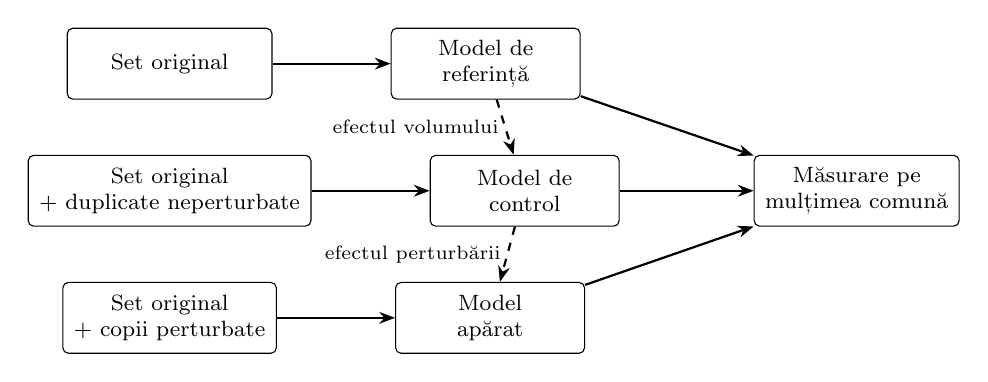
\begin{tikzpicture}[node distance=7mm and 15mm]
        \node[blocmare] (s1) {Set original};
        \node[blocmare, below=of s1] (s2) {Set original\\ + duplicate neperturbate};
        \node[blocmare, below=of s2] (s3) {Set original\\ + copii perturbate};

        \node[bloc, right=of s1, minimum width=24mm] (m1) {Model de\\ referință};
        \node[bloc, right=of s2, minimum width=24mm] (m2) {Model de\\ control};
        \node[bloc, right=of s3, minimum width=24mm] (m3) {Model\\ apărat};

        \node[blocmare, right=17mm of m2] (masura) {Măsurare pe\\ mulțimea comună};

        \draw[sageata] (s1) -- (m1);
        \draw[sageata] (s2) -- (m2);
        \draw[sageata] (s3) -- (m3);
        \draw[sageata] (m1) -- (masura);
        \draw[sageata] (m2) -- (masura);
        \draw[sageata] (m3) -- (masura);

        \draw[punctat] (m1) -- node[eticheta, left] {efectul volumului} (m2);
        \draw[punctat] (m2) -- node[eticheta, left] {efectul perturbării} (m3);
    \end{tikzpicture}
    \caption{Cele trei grupuri ale experimentului. Seturile de antrenare ale ultimelor două au același număr de rânduri și aceeași distribuție a claselor, diferă doar prin faptul că rândurile adăugate sunt sau nu perturbate. Rezultatul raportat este diferența dintre modelul apărat și cel de control, nu față de modelul de referință.}
    \label{fig:brate}
\end{figure}

\subsection{Menținerea neschimbată a funcției de cost}\label{subsec:ponderi}

Al treilea efect enumerat în subsecțiunea~\ref{subsec:confuzii} nu este eliminat de grupul de control, pentru că se manifestă identic în ambele grupuri augmentate, dar el trebuie totuși neutralizat pentru ca acestea să rămână comparabile cu modelul de referință.

Modelele antrenate în condiții de dezechilibru sever folosesc ponderi de clasă invers proporționale cu frecvența observată, conform argumentului din secțiunea~\ref{sec:metrici}. Dacă aceste ponderi ar fi recalculate pe setul augmentat, ele ar avea alte valori decât cele folosite de modelul de referință, iar cele două modele ar diferi atât prin datele de antrenare, cât și prin funcția minimizată. Soluția adoptată este calcularea ponderilor o singură dată, pe etichetele setului original, și transmiterea aceluiași set de valori tuturor grupurilor. Augmentarea schimbă astfel numai datele, nu și obiectivul.


\subsection{Proveniența statisticilor folosite la generare}\label{subsec:provenienta}

Generatorul de variante are nevoie, pentru caracteristicile care nu pot fi recalculate din fluxul izolat, de statistici extrase din datele observate, conform delimitării din subsecțiunea~\ref{subsec:interval}. Atunci când modelele sunt înghețate, aceste statistici pot fi construite din ambele partiții: ele descriu comportamentul senzorului, adică o proprietate a procesului de generare a datelor, iar nimic nu se antrenează pe ele.

În momentul în care variantele perturbate devin date de antrenare, situația se schimbă calitativ. O statistică derivată din partiția de test s-ar regăsi atunci, indirect, în valorile pe care modelul le vede la antrenare, ceea ce ar constitui o scurgere de informație dinspre setul de evaluare către model. Din acest motiv, generarea datelor de antrenare folosește exclusiv statistici construite din partiția de antrenare.

Distincția este între două roluri diferite ale aceluiași mecanism, nu o inconsecvență. Generarea variantelor pe care se măsoară evaziunea continuă să folosească statisticile complete, pentru ca modificările măsurate să fie identice cu cele din etapele anterioare și rezultatele să rămână comparabile. Acolo, modelele sunt deja antrenate și nu mai pot fi influențate. Restricția se aplică numai generării datelor de antrenare. Consecința practică este că generatorul dispune, în acest al doilea rol, de un tabel de corespondențe mai sărac, deci recurge mai des la valorile de rezervă, iar acest lucru trebuie raportat.

\subsection{Numitorul comun al comparației}\label{subsec:cohorta}

Rata de evaziune se calculează, conform subsecțiunii~\ref{subsec:eligibil}, exclusiv peste fluxurile pe care modelul le semnalează pe traficul nemodificat. Această restricție este necesară, dar creează o dificultate atunci când se compară modele diferite: fiecare model semnalează o mulțime proprie de fluxuri, deci fiecare rată se raportează la o populație proprie.

Consecința este că două procente obținute de modele diferite nu sunt direct comparabile. Un model care semnalează mai puține fluxuri pe traficul nemodificat are un numitor mai mic. Dacă fluxurile pe care nu le mai semnalează sunt tocmai cele ușor de perturbat, rata lui de evaziune scade fără ca robustețea să fi crescut. Comparația ar înregistra atunci o îmbunătățire produsă de o pierdere de sensibilitate.

Soluția este fixarea în prealabil a unei mulțimi comune de fluxuri, formată din intersecția fluxurilor semnalate de toate modelele comparate, la toate repetările experimentului. Pe această mulțime, care nu se modifică de la un model la altul, ratele se măsoară pe exact aceleași fluxuri și devin comparabile pereche cu pereche. Mărimea mulțimii trebuie raportată împreună cu ratele: un procent calculat pe o mulțime restrânsă nu are aceeași greutate ca unul calculat pe o mulțime largă, iar o mulțime care s-a micșorat drastic este ea însăși un rezultat, semnalând că modelele comparate au ajuns să semnaleze fluxuri diferite.

Rămâne de precizat ce valoare se reține atunci când se compară două modele pe întreaga grilă de transformări. Media peste variante ar fi înșelătoare, întrucât atacatorul nu alege o transformare la întâmplare, ci pe cea care îi convine. Valoarea reținută este, prin urmare, maximul peste variantele admisibile: o apărare care reduce media, dar lasă neatinsă o singură variantă eficientă, nu a apărat nimic.

\subsection{Criterii stabilite înaintea rulării}\label{subsec:preinregistrare}

Ultimul element al construcției privește modul în care se decide dacă rezultatul este sau nu un succes. Dacă pragurile sunt alese după ce cifrele sunt cunoscute, ele pot fi ajustate, conștient sau nu, astfel încât rezultatul obținut să le satisfacă. Pragurile sunt de aceea fixate înainte de rulare și consemnate împreună cu restul configurației.

Trei condiții sunt formulate în acest fel. Prima privește câștigul de robustețe și este exprimată ca îmbunătățire față de grupul de control, nu ca prag absolut. Motivul este că un prag absolut ar putea marca drept eșec un rezultat valoros: o reducere a evaziunii de la o valoare foarte mare la una încă ridicată rămâne o observație importantă, chiar dacă nu atinge un nivel considerat acceptabil în practică. A doua condiție privește costul pe traficul nemodificat și limitează scăderea admisă a performanței globale. A treia este o condiție de siguranță și cere ca nicio clasă de atac să nu piardă mai mult decât un prag stabilit din capacitatea de a fi detectată. Ea există pentru că o apărare poate consolida clasa cea mai vizibilă degradând clasele rare, iar o metrică globală ar ascunde acest lucru.

Pe lângă aceste criterii este stabilită și o valoare de referință, care indică nivelul de performanță urmărit în practică, fără a condiționa validitatea experimentului. Dacă rezultatele nu ating criteriile stabilite, acest lucru arată că metoda de antrenare evaluată nu reduce suficient efectul transformărilor analizate. Un asemenea rezultat rămâne relevant, chiar dacă nu confirmă eficiența metodei.

\section{Structura logică și funcțională a soluției}\label{sec:structura}

Din elementele teoretice anterioare rezultă o descompunere funcțională în șase module, cu dependențe strict secvențiale. Fluxul de date este prezentat în figura~\ref{fig:pipeline}.

\begin{figure}[!ht]
    \centering
    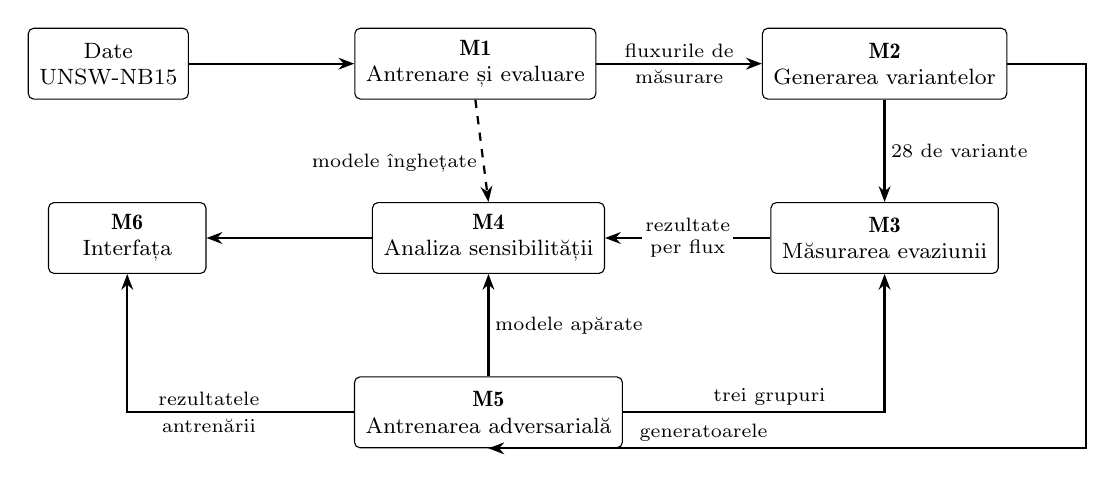
\begin{tikzpicture}[node distance=8mm and 21mm]
        \node[bloc, minimum width=20mm] (date) {Date\\ UNSW-NB15};
        \node[blocmare, right=of date] (m1) {\textbf{M1}\\ Antrenare și evaluare};
        \node[blocmare, right=of m1] (m2) {\textbf{M2}\\ Generarea variantelor};
        \node[blocmare, below=13mm of m2] (m3) {\textbf{M3}\\ Măsurarea evaziunii};
        \node[blocmare, left=of m3] (m4) {\textbf{M4}\\ Analiza sensibilității};
        \node[bloc, left=of m4, minimum width=20mm] (m6) {\textbf{M6}\\ Interfața};
        \node[blocmare, below=13mm of m4] (m5) {\textbf{M5}\\ Antrenarea adversarială};

        \draw[sageata] (date) -- (m1);
        \draw[sageata] (m1) -- node[eticheta, above] {fluxurile de} node[eticheta, below] {măsurare} (m2);
        \draw[sageata] (m2) -- node[eticheta, right] {28 de variante} (m3);
        \draw[sageata] (m3) -- node[eticheta, midway, align=center, fill=white, inner sep=1pt] {rezultate\\ per flux} (m4);
        \draw[sageata] (m4) -- (m6);
        \draw[sageata] (m5.west) -| node[eticheta, pos=0.32, above] {rezultatele} node[eticheta, pos=0.32, below] {antrenării} (m6.south);
        \draw[sageata] (m2.east) -- ++(10mm,0) |- node[eticheta, pos=0.82, above] {generatoarele} (m5.south);
        \draw[sageata] (m5.east) -| node[eticheta, pos=0.28, above] {trei grupuri} (m3.south);
        \draw[sageata] (m5.north) -- node[eticheta, right] {modele apărate} (m4.south);

        \draw[punctat] (m1.south) -- node[eticheta, pos=0.62, left] {modele înghețate} (m4.north);
    \end{tikzpicture}
    \caption{Structura funcțională a soluției și fluxul de date între module. Săgeata punctată indică modelele înghețate din M1, folosite fără reantrenare de M4. M4 se aplică de două ori, o dată modelelor de referință și o dată celor apărate produse de M5. Interfața, M6, este singurul modul terminal, consumând atât rezultatele analizei de sensibilitate, cât și pe cele ale antrenării adversariale.}
    \label{fig:pipeline}
\end{figure}

\textbf{Modulul M1} construiește clasificatoarele și le evaluează pe traficul nemodificat, folosind metricile din secțiunea~\ref{sec:metrici}. El produce modelele antrenate și predicțiile de referință, din care se derivă mulțimea fluxurilor asupra cărora se va măsura evaziunea. După această etapă, modelele sunt considerate înghețate: niciun modul ulterior nu le modifică, ceea ce garantează că variațiile observate provin exclusiv din perturbarea intrărilor.

\textbf{Modulul M2} generează variantele perturbate. El pune în aplicare cele patru condiții din subsecțiunea~\ref{subsec:admisibile} și procedura de propagare din subsecțiunea~\ref{subsec:propagare}. Fiecare variantă generată este supusă unui set de verificări de validitate înainte de a fi transmisă mai departe. O variantă care încalcă o constrângere este respinsă, nu corectată tacit. Modulul depinde de M1 doar prin mulțimea fluxurilor de măsurat, nu prin structura modelelor.

\textbf{Modulul M3} aplică modelele înghețate variantelor perturbate și încadrează rezultatele conform taxonomiei din subsecțiunea~\ref{subsec:rezultate}, calculând ratele și intervalele. Verificarea invariantului identității precede orice altă măsurătoare. Mecanismul este invocat de două ori în cursul experimentului, o dată pentru modelele din M1 și o dată pentru cele din M5, iar cele două rulări scriu rezultate în locații separate, pentru ca ratele modelelor de referință să nu se amestece cu cele ale modelelor apărate.

\textbf{Modulul M4} calculează importanțele și fracțiunile accesibile și pune în coresponden\-ță importanța caracteristicilor afectate de fiecare transformare cu rata de evaziune produsă de acea transformare. El consumă atât modelele din M1, cât și rezultatele per flux din M3. Aceeași procedură se aplică, într-o a doua rulare, modelelor produse de M5, pentru a stabili dacă apărarea a schimbat caracteristicile pe care acestea se sprijină. Rezultatul acestei a doua rulări este prezentat în subsecțiunea~\ref{subsec:o6-mecanism}.

\textbf{Modulul M5} reia antrenarea clasificatoarelor pe seturi augmentate cu variante perturbate, conform construcției din secțiunea~\ref{sec:antrenare}. Spre deosebire de celelalte module, el nu consumă modelele înghețate, ci produce modele noi, motiv pentru care artefactele sale sunt păstrate separat și nu înlocuiesc niciodată modelele de referință. Dependența lui de M2 este una de mecanism, nu de rezultat: folosește aceleași generatoare, dar aplicate partiției de antrenare și cu statisticile restrânse conform subsecțiunii~\ref{subsec:provenienta}. Legătura cu M3 este, la rândul ei, tot una de mecanism, conform explicației de mai sus. Bucla astfel închisă nu introduce circularitate, întrucât măsurarea se face cu modelele deja antrenate și înghețate la rândul lor.

\textbf{Modulul M6} expune rezultatele într-o formă explorabilă interactiv și permite evaluarea unor combinații de parametri care nu fac parte din setul predefinit. Cerința teoretică impusă acestui modul este ca perturbările pe care le aplică să fie construite prin aceleași mecanisme ca cele din M2, iar nu printr-o realizare paralelă. Altfel, valorile afișate interactiv ar putea diverge de cele măsurate sistematic, iar modulul ar înceta să fie un instrument de explorare a acelorași rezultate. Fiind ultimul din lanț, este și singurul care afișează simultan rezultatele lui M4 și pe cele ale lui M5, motiv pentru care depinde de amândouă, nu doar de modulul care îl precede direct.

Dependențele dintre module sunt unidirecționale, iar fiecare tranziție este însoțită de o condiție verificabilă: varianta neperturbată generată de M2 trebuie să reproducă predicțiile de referință ale lui M1, iar rata de evaziune calculată de M3 pentru această variantă trebuie să fie nulă. Aceste condiții transformă lanțul de prelucrare într-o succesiune de etape verificabile independent, ceea ce permite localizarea unei eventuale erori la nivelul modulului care o produce.

\section{Ipotezele cadrului și limitele lor}\label{sec:ipoteze}

Cadrul teoretic construit se sprijină pe un număr de ipoteze care nu pot fi verificate în interiorul lui. Enunțarea lor explicită este necesară pentru delimitarea corectă a domeniului de valabilitate a rezultatelor.

\textbf{Ipoteza de realizabilitate.} Se presupune că orice variantă considerată admisibilă corespunde unui trafic pe care atacatorul îl poate genera efectiv. Condițiile din subsecțiunea~\ref{subsec:admisibile} sunt construite pentru a garanta acest lucru, dar garanția rămâne una deductivă: ea decurge din interpretarea fiecărei caracteristici, nu dintr-o verificare experimentală. O confirmare completă ar presupune generarea traficului modificat, trecerea lui printr-un senzor real și compararea rezumatului rezultat cu cel obținut prin propagare. Această verificare depășește cadrul lucrării, iar rezultatele trebuie citite ca fiind condiționate de ipoteză.

\textbf{Ipoteza privind forma relațiilor derivate.} Observația centrală din subsecțiun\-ea~\ref{subsec:propagare} presupune că fiecare caracteristică derivată se obține ca raport a două mărimi de bază, înmulțit cu o constantă necunoscută, dar aceeași pentru toate fluxurile. Ipoteza este verificabilă indirect, prin măsurarea degradării relațiilor dintre mărimi după propagare, dar nu poate fi demonstrată în absența specificației complete a senzorului. Acolo unde forma presupusă ar fi greșită, propagarea ar introduce o abatere sistematică, mărimea acestei abateri este însă observabilă și raportabilă.

\textbf{Ipoteza de invarianță a procedurii de extragere.} Se presupune că senzorul calculează caracteristicile în același mod pentru traficul original și pentru cel perturbat. Ipoteza este rezonabilă pentru mărimile calculate din fluxul însuși, dar devine problematică pentru cele care depind de context, motiv pentru care acestea din urmă sunt tratate prin delimitarea din subsecțiunea~\ref{subsec:interval} în loc de a fi recalculate.

\textbf{Ipoteza de reprezentativitate a setului de date.} Concluziile privind ce caracteristici sunt importante pentru un model se referă la modelul antrenat pe acest set, nu la clasa de modele în general. Dacă o caracteristică are, în setul utilizat, o corelație cu eticheta care provine din modul de generare a datelor și nu din natura atacurilor, atunci dependența modelului de acea caracteristică este un artefact al setului. Cadrul propus nu poate distinge singur între cele două situații, iar distincția necesită analiza separată a provenienței datelor.

\textbf{Ipoteza de neadaptivitate.} Modelul de amenințare din subsecțiunea~\ref{subsec:acces} exclude orice interacțiune între atacator și sistemul de detecție. Un atacator cu acces la răspunsurile modelului ar putea căuta perturbări mai eficiente decât cele dintr-un set predefinit. Rezultatele obținute în acest cadru constituie, prin urmare, estimări conservatoare ale vulnerabilității: ele indică ce se poate obține fără nicio cunoaștere a apărării, nu limita superioară a ceea ce se poate obține.

\textbf{Adaptarea atacatorului nu este evaluată.}
După reantrenare, modelul este testat folosind aceleași tipuri de transformări considerate anterior. Evaluarea nu analizează situația în care atacatorul observă efectul apărării și își modifică strategia. Prin urmare, reducerea ratei de evaziune arată că modelul a devenit mai rezistent la transformările evaluate, dar nu demonstrează robustețea sa față de alte strategii de atac.

\textbf{Generalizarea la transformări noi nu este evaluată separat.}
Utilizarea acelorași tipuri de transformări atât la antrenare, cât și la testare nu permite stabilirea măsurii în care modelul poate rezista unor perturbări diferite. O asemenea verificare ar necesita excluderea unui tip de transformare din setul de antrenare și utilizarea sa numai în etapa de evaluare. În absența acestui experiment, concluziile privind eficiența antrenării se limitează la familiile de transformări incluse în studiu.

Ultima observație privind neadaptivitatea este cea mai importantă pentru interpretarea corectă a rezultatelor. O rată de evaziune ridicată măsurată în acest cadru constituie o dovadă solidă de vulnerabilitate, întrucât a fost obținută în condițiile cele mai defavorabile atacatorului. O rată scăzută, în schimb, nu constituie o dovadă de robustețe, ci doar absența unei vulnerabilități la clasa specifică de transformări evaluate.
 % \chapter{Analiză și Fundamentare Teoretică}

\chapter{Proiectare de detaliu și implementare}\label{ch:proiectare}
\pagestyle{fancy}

Acest capitol prezintă implementarea soluției fundamentate în capitolul~\ref{ch:analysis}. Sunt descrise organizarea modulară a codului, structurile de date utilizate în fiecare etapă, algoritmii implementați și principalele decizii determinate de particularitățile datelor și ale bibliotecilor folosite. Pentru fiecare decizie sunt prezentate și criteriile care au stat la baza ei, cu scopul de a facilita înțelegerea și dezvoltarea ulterioară a aplicației.

\section{Arhitectura generală a soluției}\label{sec:arhitectura}

\subsection{Principii de organizare}\label{subsec:principii}

Organizarea codului respectă trei principii, impuse de natura experimentală a lucrării.

\textbf{Separarea logicii de execuție.} Întreaga logică se află într-un pachet de biblioteci, iar scripturile executabile din rădăcina proiectului conțin doar apelul etapei corespunzătoare. Un script are, în medie, sub o sută de linii și nu implementează nimic propriu. Consecința practică este că orice funcționalitate poate fi apelată independent, atât din alt script, cât și din interfața interactivă, fără duplicarea codului.

\textbf{Etape reluabile independent.} Fiecare etapă își persistă rezultatele pe disc într-un format tabelar, iar etapa următoare le citește de acolo. O etapă poate fi astfel reluată fără a le relua pe cele anterioare, ceea ce este esențial într-un context în care antrenarea modelelor durează zeci de minute, iar analizele ulterioare sunt reluate frecvent.

\textbf{Model unic de acces la predicție.} Toate predicțiile trec printr-un singur modul, indiferent de model și de etapă. Motivul este detaliat în subsecțiunea~\ref{subsec:inferenta}: fără această centralizare, două etape ar putea obține predicții diferite pentru același flux, ceea ce ar invalida măsurătoarea.

\subsection{Structura pe pachete}\label{subsec:pachete}

Codul este organizat în pachetele prezentate în tabelul~\ref{tab:pachete}. Gruparea urmează etapele conceptuale din secțiunea~\ref{sec:structura}, nu tipurile de obiecte, astfel încât modificarea unei etape să fie localizată într-un singur director.

\begin{table}[H]
    \caption{Organizarea codului pe pachete și responsabilitățile acestora}
    \centering
    \begin{tabular}{|l|p{8.4cm}|}
        \hline
        \textbf{Pachet} & \textbf{Responsabilitate} \\
        \hline
        Nucleu & Configurație, încărcarea datelor, preprocesare, definirea modelelor, evaluare, analiză exploratorie, utilitare comune \\
        \hline
        Inferență & Punct unic de predicție pentru toate modelele \\
        \hline
        Rețea neuronală & Arhitectura, preprocesarea specifică, bucla de antrenare, adaptorul de predicție \\
        \hline
        Perturbare & Schema caracteristicilor, generatoarele de transformări, propagarea dependențelor, componenta de validare \\
        \hline
        Evaziune & Măsurarea rezultatelor, taxonomia, agregarea, generarea figurilor \\
        \hline
        Sensibilitate & Importanța prin permutare, corelarea cu evaziunea, analiza destinațiilor \\
        \hline
        Antrenare adversarială & Construirea seturilor augmentate, grupurile de antrenare,
        evaluarea pe mulțimea comună, fișa de reproductibilitate \\
        \hline
        Interfață & Aplicația interactivă și adaptorul de perturbare live \\
        \hline
    \end{tabular}
    \label{tab:pachete}
\end{table}

Structura de dependențe este reprezentată în figura~\ref{fig:pachete}.

Dependențele sunt, cu o singură excepție, unidirecționale: pachetele de nivel superior importă din cele inferioare, niciodată invers. Scripturile de rulare nu sunt importate de nimeni, iar pachetele de interfață și de antrenare adversarială sunt și ele consumatori finali. Antrenarea adversarială este singura care produce modele noi, motiv pentru care scrie exclusiv în directoare proprii.

Excepția merită enunțată, pentru că o diagramă care ar ascunde-o ar descrie altceva decât codul. Modulul de inferență, aflat în nucleu, are nevoie de clasa care încarcă rețeaua neuronală, iar aceasta din urmă importă la rândul ei din nucleu, deci cele două pachete se referă reciproc. Ciclul nu produce însă o eroare la încărcare, întrucât importul din nucleu către rețea se execută în interiorul funcției care îl folosește, nu la nivelul modulului. Alegerea are și un al doilea motiv, practic: etapele care lucrează exclusiv cu ansamblurile de arbori nu încarcă astfel biblioteca de învățare profundă, care este de departe cea mai costisitoare dependență a proiectului.

\begin{figure}[!h]
    \centering
    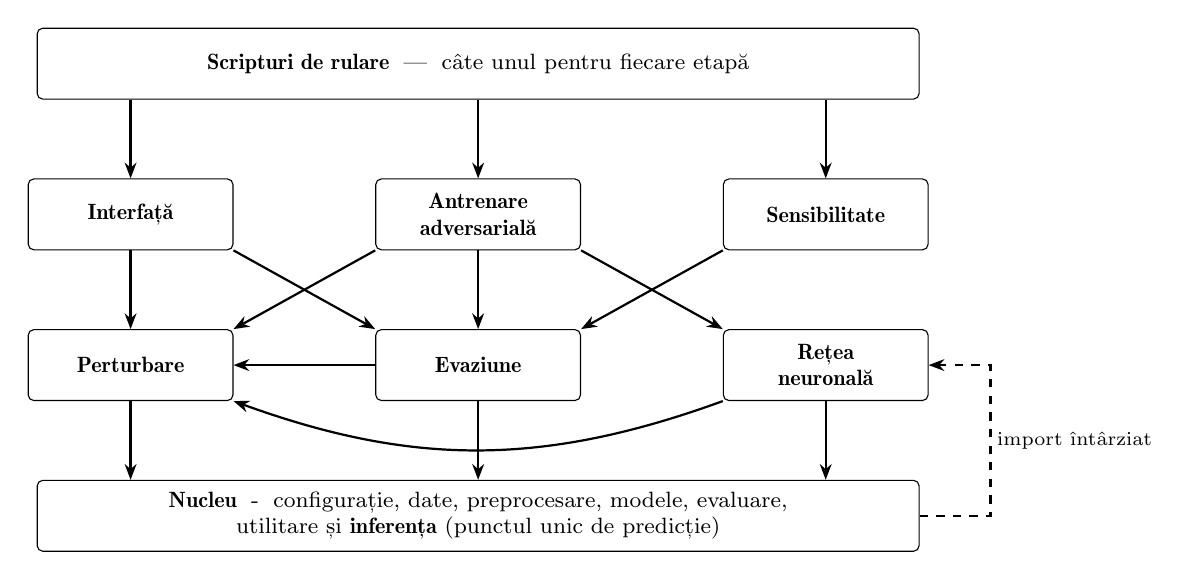
\begin{tikzpicture}[node distance=8mm and 9mm]
        \node[bloc, minimum width=112mm] (scripturi)
            {\textbf{Scripturi de rulare} \;---\; câte unul pentru fiecare etapă};

        \node[bloc, minimum width=26mm, below=10mm of scripturi] (adv)
            {\textbf{Antrenare}\\ \textbf{adversarială}};
        \node[bloc, minimum width=26mm, left=18mm of adv] (ui) {\textbf{Interfață}};
        \node[bloc, minimum width=26mm, right=18mm of adv] (sens) {\textbf{Sensibilitate}};

        \node[bloc, minimum width=26mm, below=10mm of adv] (evaz) {\textbf{Evaziune}};
        \node[bloc, minimum width=26mm, below=10mm of ui] (pert) {\textbf{Perturbare}};
        \node[bloc, minimum width=26mm, below=10mm of sens] (retea)
            {\textbf{Rețea}\\ \textbf{neuronală}};

        \node[bloc, minimum width=112mm, below=10mm of evaz] (nucleu)
            {\textbf{Nucleu} \;-\; configurație, date, preprocesare, modele, evaluare,\\
             utilitare și \textbf{inferența} (punctul unic de predicție)};

        \draw[sageata] (scripturi.south -| ui) -- (ui);
        \draw[sageata] (scripturi) -- (adv);
        \draw[sageata] (scripturi.south -| sens) -- (sens);

        \draw[sageata] (ui) -- (pert);
        \draw[sageata] (ui.south east) -- (evaz.north west);
        \draw[sageata] (adv) -- (evaz);
        \draw[sageata] (adv.south west) -- (pert.north east);
        \draw[sageata] (adv.south east) -- (retea.north west);
        \draw[sageata] (sens.south west) -- (evaz.north east);
        \draw[sageata] (retea) -- (nucleu.north -| retea);
        \draw[sageata] (evaz) -- (nucleu.north -| evaz);
        \draw[sageata] (pert) -- (nucleu.north -| pert);
        \draw[sageata] (evaz) -- (pert);
        \draw[sageata] (retea.south west) to[out=200, in=340] (pert.south east);

        \draw[punctat] (nucleu.east) -- ++(9mm,0) |-
            node[eticheta, pos=0.25, right] {import întârziat} (retea.east);
    \end{tikzpicture}
    \caption{Dependențele reale dintre pachete, extrase din instrucțiunile de import. Săgețile continue merg de sus în jos: fiecare pachet importă din cele situate sub el. Singura excepție este săgeata punctată, prin care nucleul ajunge la rețeaua neuronală; ea închide un ciclu, evitat în practică prin efectuarea importului abia în momentul apelului, nu la încărcarea modulului.}
    \label{fig:pachete}
\end{figure}

\subsection{Configurația centralizată}\label{subsec:configuratie}

Toate constantele experimentului sunt declarate într-un singur modul de configu\-rație: căile către date și rezultate, \textit{seed}-ul generatorului de numere aleatoare, hiperparametrii celor trei modele, taxonomia caracteristicilor din tabelul~\ref{tab:taxonomie}, nivelurile de perturbare, pragurile de validitate fizică și denumirile categoriilor de rezultat.

Într-un experiment în care aceeași constantă este folosită de mai multe etape rulate la momente diferite, o valoare duplicată în două locuri conduce la rezultate care par valide, dar provin din configurații diferite. Un exemplu concret îl constituie valoarea TTL asociată traficului legitim, folosită simultan de generatorul de perturbări, de mecanismul de rezolvare a contorului de context și de interfața interactivă. Declararea ei într-un singur loc garantează că cele trei componente se referă la aceeași valoare.

Modulul conține, în plus, comentarii extinse care documentează motivul fiecărei alegeri neevidente, de exemplu, de ce nivelurile TTL sunt exact cele alese, sau de ce predicția se execută pe un singur fir de execuție. Aceste comentarii constituie, în practică, jurnalul deciziilor experimentale.

\subsection{Fluxul de execuție}\label{subsec:flux}

Etapele se execută în ordinea din tabelul~\ref{tab:etape}. Ordinea este impusă de dependențele de date: fiecare etapă consumă ieșirile celei precedente.

\begin{table}[H]
    \caption{Etapele de execuție, dependențele și rezultatele produse}
    \centering
    \begin{tabular}{|l|p{3.3cm}|p{4.2cm}|}
        \hline
        \textbf{Etapă} & \textbf{Consumă} & \textbf{Produce} \\
        \hline
        Antrenarea ansamblurilor & Setul de date brut & Modele salvate, metrici, predicții de referință \\
        \hline
        Antrenarea rețelei & Setul de date brut & Model salvat, metrici, predicții de referință \\
        \hline
        Generarea variantelor & Predicțiile de referință & Manifest, raport de validitate, eșantioane \\
        \hline
        Măsurarea evaziunii & Modelele, variantele & Rate, intervale, rezultate per flux \\
        \hline
        Analiza sensibilității & Modelele, rezultatele per flux & Importanțe, corelații, figuri \\
        \hline
        Antrenarea adversarială & Setul de date brut, generatoarele de variante & Modele per grup, mulțimea comună, verdictul față de criterii \\
        \hline
        Interfața & Toate cele anterioare & Explorare interactivă \\
        \hline
    \end{tabular}
    \label{tab:etape}
\end{table}

Etapa de antrenare a rețelei neuronale este independentă de cea a ansamblurilor de arbori și poate fi executată în orice ordine față de aceasta. Ambele trebuie însă să preceadă generarea variantelor, deoarece mulțimea eligibilă se calculează din predicțiile de referință ale tuturor modelelor.

Antrenarea adversarială ocupă o poziție aparte în această succesiune. Ea consumă datele brute și mecanismul de generare, nu rezultatele etapelor de măsurare, deci ar putea fi executată imediat după prima etapă. Este plasată totuși la sfârșit, din două motive: comparația pe care o produce are sens numai raportată la vulnerabilitatea deja măsurată, iar criteriile după care se judecă rezultatul se formulează pornind de la valorile obținute în etapele anterioare. Fiind singura etapă care produce modele noi, ea scrie exclusiv în directoare proprii, astfel încât toate rezultatele precedente rămân valabile după rulare.

\section{Încărcarea și pregătirea datelor}\label{sec:date}

\subsection{Setul de date și partiționarea}\label{subsec:setdate}

Se utilizează setul UNSW-NB15 \cite{moustafa2015unsw}, în partiția oficială pusă la dispoziție de autori, cu 175\,341 de înregistrări pentru antrenare și 82\,332 pentru testare. Partiția oficială este preferată unei împărțiri proprii din două motive: rezultatele devin comparabile cu cele raportate în literatură, iar împărțirea aleatoare a unui set de trafic poate plasa fluxuri provenite din aceeași sesiune în ambele partiții, producând o scurgere de informație greu de detectat.

Fiecare înregistrare conține 45 de coloane: un identificator, 42 de caracteristici predictive (39 numerice și 3 categorice) și două etichete, una binară și una cu categoria de atac. Cifra de 42 folosită în toată lucrarea se referă la caracteristicile predictive, adică la coloanele rămase după excluderea identificatorului și a celor două etichete. Se folosește exclusiv eticheta multi-clasă, cu zece valori posibile. Coloana de identificator este păstrată separat de caracteristici: ea nu intră niciodată în model, dar este necesară pentru a putea urmări un flux individual de-a lungul întregului lanț de prelucrare, de la predicția de referință până la rezultatul perturbării.

Modulul de încărcare validează la fiecare apel prezența coloanelor așteptate și consistența tipurilor, semnalând o eroare explicită în locul unei erori tardive apărute în etapa de antrenare.

\subsection{Analiza exploratorie}\label{subsec:eda}

Etapa de analiză exploratorie produce caracterizările numerice și grafice ale setului de date. Ea raportează distribuția claselor și raportul de dezechilibru, cardinalitatea variabilelor categorice împreună cu numărul de categorii aflate sub pragul de raritate, tabelul asimetriei distribuțiilor numerice și corelațiile dintre caracteristicile numerice și etichetă.

Trei figuri sunt generate și salvate pentru a fi citate în capitolul de rezultate: distribuția claselor pe scară logaritmică, corelațiile cu eticheta și histogramele caracteristicilor cu cea mai pronunțată asimetrie. Scara logaritmică este necesară pentru prima figură, întrucât raportul dintre clasa cea mai frecventă și cea mai rară face ca, pe scară liniară, clasele minoritare să fie invizibile.

Transformarea logaritmică aplicată histogramelor este folosită \emph{exclusiv} pentru lizibilitatea reprezentării grafice și nu intră în fluxul de modelare. Motivul este cel discutat în subsecțiunea~\ref{subsec:arbori}: o transformare monotonă aplicată independent fiecărei caracteristici nu modifică deciziile unui ansamblu de arbori, deci nu ar avea niciun efect asupra rezultatelor, iar aplicarea ei doar pentru unele modele ar introduce o diferență inutilă între condițiile experimentale.

\subsection{Gruparea categoriilor rare}\label{subsec:rare}

Variabila care descrie protocolul are 133 de valori distincte, cu o distribuție puternic dezechilibrată: primele două valori acoperă împreună peste jumătate din observații, în timp ce 118 dintre ele apar de mai puțin de 200 de ori fiecare. Codificarea directă prin variabile indicator produce astfel o matrice cu peste o sută de coloane aproape constante, ceea ce ridică riscul supraînvățării unor categorii cu suport statistic redus.

S-a implementat, deci, un transformator care grupează categoriile rare. La ajustare, el reține pentru fiecare coloană categorică mulțimea valorilor care apar de cel puțin un număr prestabilit de ori în datele de antrenare. La transformare, orice valoare din afara acestei mulțimi este înlocuită cu o etichetă rezervată. Pragul folosit este de 50 de apariții. Transformatorul este integrat în fluxul de preprocesare \emph{înaintea} codificării, astfel încât să fie salvat împreună cu modelul și să se aplice identic la reîncărcare.

\begin{verbatim}
class RareCategoryGrouper(BaseEstimator, TransformerMixin):
    """Inlocuieste categoriile rare sau necunoscute."""

    def fit(self, X, y=None):
        # Multimea retinuta se calculeaza EXCLUSIV pe datele primite
        # la ajustare, adica pe partitia de antrenare.
        self.keep_ = {
            col: set(X[col].value_counts()
                     [lambda s: s >= self.min_freq].index)
            for col in self.columns
        }
        return self

    def transform(self, X):
        X = X.copy()
        for col in self.columns:
            # Acelasi test prinde si categoriile rare din train,
            # si pe cele nevazute: ambele cad in afara multimii.
            X[col] = X[col].where(X[col].isin(self.keep_[col]),
                                  self.other_label)
        return X
\end{verbatim}

Separarea dintre cele două metode este esențială. Mulțimea valorilor păstrate
se stabilește în \texttt{fit}, exclusiv din datele de antrenare, și rămâne
fixată după aceea. Partiția de testare trece doar prin \texttt{transform}, deci
nu poate influența ce categorii sunt considerate frecvente. O implementare care
ar recalcula mulțimea la fiecare transformare ar produce o scurgere de
informație dinspre setul de testare, greu de observat în rezultate.

Al doilea aspect este că nu există o ramură separată pentru categoriile
nevăzute. Un singur test, apartenența la \texttt{keep\_}, tratează deopotrivă o
categorie rară din antrenare și o valoare care apare pentru prima dată la
inferență, întrucât niciuna dintre ele nu se află în mulțimea învățată.

Efectul cantitativ al grupării trebuie raportat corect, întrucât este mai mic decât sugerează cardinalitatea inițială. La pragul ales, doar trei protocoale sunt colapsate, iar lățimea codificării acestei coloane scade de la 133 la 131 de poziții. Motivul este că lungul șir de categorii rare nu coboară, în general, sub pragul de 50: majoritatea protocoalelor apar de ordinul a o sută de ori, ceea ce reflectă modul sintetic în care a fost generat traficul. Reducerea dimensionalității nu constituie, prin urmare, principalul beneficiu al mecanismului în acest set de date.

Variabila care descrie starea conexiunii conține în partiția de testare două valori care nu apar deloc în cea de antrenare. Fără o tratare explicită, codificatorul le-ar transforma tăcut într-un vector nul, comportament corect din punct de vedere tehnic, dar complet invizibil în raportare. Prin grupare, aceste valori sunt încadrate explicit în categoria rezervată, iar situația devine observabilă și documentată. Mecanismul a fost păstrat, prin urmare, pentru corectitudinea și transparența tratării categoriilor nevăzute, nu pentru compresia spațiului de caracteristici.

\subsection{Fluxul de preprocesare}\label{subsec:preprocesare}

Preprocesarea este încapsulată într-un flux compus, ceea ce garantează că aceleași transformări se aplică identic la antrenare și la predicție. Structura este comună celor două ansambluri de arbori: gruparea categoriilor rare, apoi codificarea prin variabile indicator a coloanelor categorice, cu transmiterea nemodificată a celor numerice.

Absența normalizării valorilor numerice este o decizie deliberată, justificată în subsecțiunea~\ref{subsec:arbori}. Codificatorul păstrează, suplimentar, tratarea valorilor nevăzute ca plasă de siguranță, chiar dacă gruparea prealabilă ar trebui să le elimine.

Rețeaua neuronală folosește un flux diferit, descris în subsecțiunea~\ref{subsec:retea}. Diferența privește exclusiv reprezentarea internă a valorilor, în timp ce mulțimea caracteristicilor, împărțirea în partiții și etichetele rămân identice.

\section{Implementarea clasificatoarelor}\label{sec:clasificatoare}

\subsection{Ansamblurile de arbori}\label{subsec:ansambluri}

Cele două ansambluri sunt construite peste fluxul de preprocesare comun. Random Forest folosește 200 de arbori și ponderarea claselor invers proporțională cu frecvența lor. Modelul cu XGBoost folosește 300 de arbori, adâncime maximă 8, rată de învățare 0{,}1 și eșantionare a rândurilor la fiecare iterație.

Ponderarea claselor necesită tratamente diferite la cele două biblioteci. În primul caz este disponibil un parametru dedicat. În al doilea, ponderile se calculează explicit și se transmit ca vector de ponderi per observație la apelul de antrenare. Rezultatul este echivalent, dar diferența de interfață trebuie cunoscută la întreținere.

O particularitate de implementare merită semnalată: biblioteca de XGBoost necesită etichete codificate numeric, în timp ce restul lanțului lucrează cu etichete textuale. Conversia este încapsulată împreună cu modelul, iar maparea inversă este salvată alături de acesta, astfel încât predicțiile expuse în exterior să fie întotdeauna textuale. Fără această încapsulare, ordinea claselor ar deveni o convenție implicită, ușor de încălcat la o modificare ulterioară.

După antrenare, fiecare model este salvat pe disc, apoi reîncărcat și verificat: predicțiile modelului reîncărcat trebuie să coincidă cu cele ale modelului din memorie. Verificarea prinde erorile de serializare, care altfel s-ar manifesta abia în etapele următoare, sub forma unor rezultate inexplicabile.

\subsection{Transformer}\label{subsec:retea}

Mecanismul de atenție este scris de la zero, nu preluat din componentele gata făcute ale bibliotecii de învățare profundă. Alegerea costă mai mult cod, dar aduce două lucruri pe care varianta scurtă nu le oferă: fiecare operație descrisă în subsecțiunea~\ref{subsec:atentie} apare explicit și poate fi verificată separat, iar ponderile de atenție rămân accesibile din exterior, în loc să rămână închise într-o componentă opacă. A doua proprietate este cea care face posibilă inspectarea a ceea ce modelul consideră relevant într-un flux dat.

\textbf{Tokenizatorul de caracteristici} transformă vectorul de intrare într-o secvență de reprezentări. Fiecare coloană numerică primește un vector de ponderi și unul de deplasare proprii, astfel încât valoarea scalară a coloanei este proiectată într-un spațiu de dimensiune 192 printr-o transformare afină învățată separat pentru fiecare coloană. Fiecare coloană categorică primește un tabel de reprezentări indexat după valoarea categoriei. Se adaugă un vector de agregare, inițializat aleator și învățat, care va colecta informația din întreaga secvență. Inițializarea tuturor parametrilor este uniformă, cu limite invers proporționale cu rădăcina dimensiunii reprezentării, ca în lucrarea de referință \cite{gorishniy2021revisiting}.

Structura completă a rețelei este prezentată în figura următoare, iar implementarea mecanismului de atenție este reprodusă în secțiunea~\ref{sec:anexa-atentie}.

\begin{figure}[!ht]
    \centering
    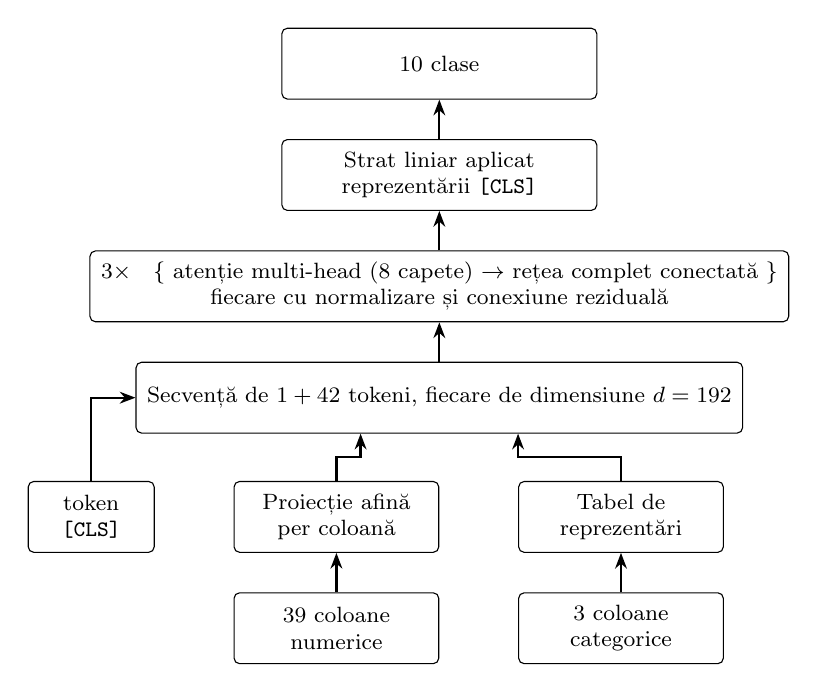
\begin{tikzpicture}[node distance=5mm and 6mm]
        \node[bloc, minimum width=26mm] (num) {39 coloane\\ numerice};
        \node[bloc, minimum width=26mm, right=10mm of num] (cat) {3 coloane\\ categorice};
        \node[bloc, minimum width=26mm, above=of num] (proj) {Proiecție afină\\ per coloană};
        \node[bloc, minimum width=26mm, above=of cat] (emb) {Tabel de\\ reprezentări};
        \node[bloc, minimum width=16mm, left=10mm of proj] (cls) {token\\ \texttt{[CLS]}};
        \node[bloc, minimum width=74mm, above=6mm of proj.north east, anchor=south] (seq)
            {Secvență de $1 + 42$ tokeni, fiecare de dimensiune $d = 192$};
        \node[bloc, minimum width=74mm, above=of seq] (blocuri)
            {$3 \times$ \; \{ atenție multi-head (8 capete) $\rightarrow$ rețea complet conectată \}\\
             fiecare cu normalizare și conexiune reziduală};
        \node[bloc, minimum width=40mm, above=of blocuri] (head) {Strat liniar aplicat\\ reprezentării \texttt{[CLS]}};
        \node[bloc, minimum width=40mm, above=of head] (out) {10 clase};

        \draw[sageata] (num) -- (proj);
        \draw[sageata] (cat) -- (emb);
        \draw[sageata] (proj.north) -- ++(0,3mm) -| ($(seq.south)+(-10mm,0)$);
        \draw[sageata] (emb.north) -- ++(0,3mm) -| ($(seq.south)+(10mm,0)$);
        \draw[sageata] (cls.north) |- ($(seq.west)+(-2mm,0)$) -- (seq.west);
        \draw[sageata] (seq) -- (blocuri);
        \draw[sageata] (blocuri) -- (head);
        \draw[sageata] (head) -- (out);
    \end{tikzpicture}
    \caption{Arhitectura modelului Transformer. Fiecare caracteristică devine un token, iar clasificarea se face din reprezentarea finală a tokenului de agregare.}
    \label{fig:transformer}
\end{figure}

\textbf{Blocul de transformare} aplică succesiv atenție multi-head cu 8 capete și o rețea complet conectată, fiecare precedată de normalizare și urmată de o conexiune reziduală. Se folosesc trei astfel de blocuri. Regularizarea se aplică diferențiat: 0{,}2 pe ponderile de atenție și 0{,}1 în rețeaua complet conectată, valorile fiind alese astfel încât capacitatea modelului să nu fie limitată excesiv pe clasele rare. Clasificarea se realizează dintr-un strat liniar aplicat reprezentării finale a vectorului de agregare. Modelul rezultat are aproximativ 789 de mii de parametri.

\textbf{Preprocesarea specifică} diferă de cea a ansamblurilor prin două aspecte. Valorile numerice sunt standardizate, din motivele expuse în subsecțiunea~\ref{subsec:atentie}. Standardizarea este ajustată exclusiv pe subsetul efectiv de antrenare, cu excluderea feliei de validare, pentru ca aceasta din urmă să rămână neinfluențată și criteriul de oprire timpurie să fie nepărtinitor. Coloanele categorice sunt convertite în indici întregi, nu în variabile indicator, întrucât sunt consumate de tabelele de reprezentări.

\textbf{Bucla de antrenare} folosește optimizatorul AdamW cu rată de învățare $10^{-4}$, regularizare $10^{-5}$ și loturi de 512 observații, pe cel mult 100 de epoci. Funcția de cost este entropia încrucișată cu ponderi per clasă, calculate din frecvențele din setul de antrenare. Se rezervă 15\% din datele de antrenare, stratificat, pentru validare.

\textbf{Selecția modelului final} constituie punctul care a necesitat cea mai atentă proiectare. Criteriul natural, păstrarea modelului cu cel mai bun scor de validare, s-a dovedit nepotrivit în acest context. Scorul macro-$F1$ de validare oscilează puternic de la o epocă la alta, deoarece este dominat de clasele rare, unde câteva observații clasificate diferit modifică sensibil media neponderată din secțiunea~\ref{sec:metrici}. Selecția pe valoarea instantanee riscă astfel să rețină un maxim conjunctural, apărut din fluctuație, în locul unui model aflat pe o traiectorie stabil ascendentă.

Soluția adoptată este selecția pe scorul \emph{netezit}: la fiecare epocă se calculează media scorurilor de validare pe o fereastră mobilă de trei epoci, iar modelul este reținut atunci când această medie se îmbunătățește. Același criteriu netezit guvernează și oprirea timpurie, cu o răbdare de 10 epoci. Procedura nu garantează un scor final mai bun, o fluctuație favorabilă poate produce, punctual, o valoare superioară, dar garantează că modelul reținut este reprezentativ pentru o regiune stabilă a traiectoriei de antrenare, ceea ce este cerința corectă atunci când modelul urmează să fie supus unor experimente ulterioare.

Antrenarea este configurată să folosească algoritmi determiniști, cu prețul unui timp de execuție cu aproximativ 7\% mai mare. Fără această constrângere, operațiile de propagare inversă prin tabelele de reprezentări produc rezultate ușor diferite între rulări, iar modelul obținut nu ar fi reproductibil.

\subsection{Stratul de inferență deterministă}\label{subsec:inferenta}

Toate predicțiile din lucrare trec printr-un modul unic, care expune aceeași interfață pentru cele trei modele și ascunde diferențele dintre biblioteci. Existența lui rezolvă o problemă descoperită experimental și care, nesoluționată, ar fi compromis măsurătoarea.

Random Forest produce, pentru un număr mic de fluxuri, predicții care variază între apeluri identice. Cauza este că decizia se ia prin însumarea voturilor arborilor, iar când primele două clase primesc un număr foarte apropiat de voturi, ordinea de însumare, care depinde de repartizarea pe fire de execuție, determină care dintre ele are valoarea finală mai mare. În setul analizat există 44 de fluxuri aflate în această situație, dintre care 43 la egalitate exactă și unul cu o diferență la limita preciziei reprezentării în virgulă mobilă.

Consecința asupra experimentului este disproporționată față de numărul de fluxuri afectate. Dacă predicția de referință și predicția pe varianta perturbată se obțin din apeluri diferite, un astfel de flux poate fi raportat ca schimbându-și clasa fără ca nimic să fi fost modificat, iar schimbarea ar fi atribuită eronat perturbării. Într-un context în care unele clase de atac au sub o sută de observații, câteva astfel de comutări false nu se pierd în zgomot.

Soluția este forțarea execuției pe un singur fir la încărcarea modelului, ceea ce elimină complet variația. Costul este o creștere a timpului de predicție de la aproximativ 0{,}4 la 1{,}2 secunde pentru întregul set de atac, neglijabilă la scara experimentului. Este important de subliniat că măsura nu modifică niciun rezultat: predicțiile obținute pe un singur fir coincid cu cele stocate anterior. Ea elimină variabilitatea, nu introduce o valoare diferită.

Modulul realizează și adaptarea rețelei neuronale la aceeași interfață, aplicând intern preprocesarea specifică și convertind ieșirile numerice în etichete textuale. Etapele ulterioare pot astfel trata cele trei modele uniform, fără ramificații condiționale.

\section{Motorul de generare a variantelor perturbate}\label{sec:motor}

\subsection{Schema caracteristicilor}\label{subsec:schema}

Un modul dedicat menține corespondența dintre numele coloanelor și categoriile din tabelul~\ref{tab:taxonomie} și expune funcții de interogare folosite de generatoare și de validatoare. Centralizarea garantează că generatorul și validatorul operează cu aceeași definiție a mulțimii caracteristicilor imuabile. În absența ei, o modificare a taxonomiei într-un singur loc ar produce un validator care aprobă variante pe care ar trebui să le respingă.

Modulul asigură și restaurarea tipurilor de date. Operațiile de propagare produc valori în virgulă mobilă chiar și pentru coloane care în setul original sunt întregi, iar diferența de tip poate modifica comportamentul codificatorului. După fiecare transformare, tipurile sunt readuse la cele ale cadrului original.

\subsection{Generatoarele de transformări}\label{subsec:generatoare}

Fiecare tip de transformare este implementat ca o funcție cu semnătură comună, care primește cadrul de intrare, nivelul de intensitate și contextul precalculat, și returnează cadrul perturbat împreună cu metadatele transformării. Uniformitatea semnăturii permite tratarea generatoarelor ca intrări într-un registru, iar adăugarea unui nou tip de transformare nu necesită modificarea codului care le apelează. Funcția care orchestrează pașii este reprodusă în secțiunea~\ref{sec:anexa-generare}.

\textbf{Transformarea TTL} atribuie valoarea TTL a pachetelor emise o valoare-țintă și declanșează rezolvarea contorului de context conform politicii selectate. Valorile-țintă sunt 64, 62 și 31, alese dintre valorile efectiv observate în captură. O valoare precum 128, deși uzuală în alte contexte, nu apare deloc în acest set și ar produce o combinație pe care modelul nu a întâlnit-o niciodată, ceea ce ar confunda efectul perturbării cu efectul extrapolării.

\textbf{Adăugarea de umplutură} (\verb|padding|) crește volumul de octeți transmiși cu o fracțiune dată. Implementarea tratează explicit limita fizică a dimensiunii pachetului: dacă mărirea pachetelor existente ar depăși unitatea maximă de transmisie, generatorul adaugă pachete suplimentare în loc să depășească limita, ceea ce modifică în mod corect și numărul de pachete, deci și mărimile derivate din el. Plafonul per pachet se calculează relativ la valoarea originală, deoarece setul conține o înregistrare a cărei dimensiune medie o depășește deja pe cea nominală.

\textbf{Dilatarea temporală} (\verb|timing|) multiplică durata fluxului cu un factor supraunitar, ceea ce antrenează prin propagare atât mărimile temporale ale sursei, cât și pe cele ale destinației, conform discuției din subsecțiunea~\ref{subsec:taxonomie}.

\textbf{Reducerea contoarelor de conexiuni} (\verb|connection_rate|) le scalează descrescător, cu un prag inferior egal cu valoarea minimă observată în date. Nivelul cel mai intens coboară contoarele direct la acest minim.

\textbf{Transformările combinate} aplică succesiv modificarea TTL, umplutura și dilatarea temporală, la intensități crescătoare, propagarea fiind executată o singură dată, la final, pentru a evita compunerea repetată a rapoartelor.

\textbf{Varianta de referință cu constrângeri relaxate} modifică suplimentar valoarea TTL a pachetelor de răspuns. Ea este marcată explicit ca nerealizabilă atât în cod, cât și în fișierele de rezultate, și este exclusă din agregările principale. Validatorul primește, pentru această singură variantă, o excepție declarată explicit, astfel încât modificarea unei coloane altfel imuabile să fie permisă doar aici și niciodată tacit.

Setul complet de variante generate este prezentat în tabelul~\ref{tab:grila}. Fiecare linie corespunde unui tip de transformare, iar numărul de niveluri determină câte variante distincte se produc.

\begin{table}[!ht]
    \caption{Grila de variante generate}
    \centering
    \begin{tabular}{|l|c|p{5.4cm}|}
        \hline
        \textbf{Tip} & \textbf{Niveluri} & \textbf{Parametri} \\
        \hline
        Identitate & 1 & Nicio modificare (control) \\
        \hline
        TTL, politică conservatoare & 3 & Valori-țintă 64, 62, 31 \\
        \hline
        TTL, politică optimistă & 3 & Valori-țintă 64, 62, 31 \\
        \hline
        Umplutură & 4 & $+10\%$, $+25\%$, $+50\%$, $+100\%$ \\
        \hline
        Temporizare & 4 & $\times 1{,}5$, $\times 2$, $\times 5$, $\times 10$ \\
        \hline
        Rată de conexiuni & 4 & $\times 0{,}75$, $\times 0{,}5$, $\times 0{,}25$, minim \\
        \hline
        Combinată, conservatoare & 4 & Intensități crescătoare \\
        \hline
        Combinată, optimistă & 4 & Intensități crescătoare \\
        \hline
        Referință relaxată & 1 & \textbf{Nerealizabilă}: atinge și TTL-ul victimei \\
        \hline
        \multicolumn{2}{|l|}{\textbf{Total}} & \textbf{28 de variante} \\
        \hline
    \end{tabular}
    \label{tab:grila}
\end{table}

Nivelul 0 este întotdeauna varianta identică și servește drept control, conform invariantului identității din subsecțiunea~\ref{subsec:rezultate}. Cele 26 de variante realizabile de la nivelurile nenule constituie baza analizei de corelație din secțiunea~\ref{sec:implsensibilitate}.

O transformare a fost eliminată în cursul dezvoltării. Modificarea parametrilor ferestrei TCP s-a dovedit lipsită de conținut: analiza datelor a arătat că această caracteristică ia o singură valoare pentru toate fluxurile care folosesc protocolul TCP și o altă valoare unică pentru restul, fără excepție. Ea nu codifică, prin urmare, nimic în plus față de protocolul însuși, iar perturbarea ei fie nu ar schimba nimic, fie ar contrazice protocolul, care este o caracteristică imuabilă. Eliminarea unei transformări lipsite de conținut este preferabilă raportării unei rate de evaziune nule obținute dintr-un motiv greșit.

\subsection{Propagarea dependențelor}\label{subsec:implpropagare}

Propagarea implementează direct observația centrală din subsecțiunea~\ref{subsec:propagare}. După ce generatorul a stabilit valorile de bază, modulul de dependențe calculează rapoartele dintre valorile noi și cele originale și le aplică multiplicativ caracteristicilor derivate, conform relațiilor din tabelul~\ref{tab:propagare}.

Tratarea numitorilor nuli este esențială pentru robustețea implementării. Împărți\-rea se execută cu o valoare de rezervă egală cu unitatea acolo unde numitorul este zero sau rezultatul nu este finit, ceea ce lasă caracteristica derivată neschimbată. Modulul raportează, pentru fiecare variantă, numărul de rânduri afectate de fiecare tip de caz degenerat, fluxuri fără octeți transmiși, cu durată nulă sau cu un singur pachet, astfel încât amploarea neutralizării să fie vizibilă în fișa rulării, nu ascunsă.

O atenție deosebită necesită intervalul mediu dintre pachete, a cărui propagare depinde de numărul de \emph{intervale}, adică de numărul de pachete minus unu. Pentru un flux cu un singur pachet, această mărime este nulă, iar raportul devine nedefinit, iar cazul este tratat separat, nu prin formula generală. Codul corespunzător se află în secțiunea~\ref{sec:anexa-propagare}.

\subsection{Rezolvarea contorului de context}\label{subsec:ct}

Contorul care combină starea conexiunii cu valorile TTL nu poate fi recalculat, conform argumentului din subsecțiunea~\ref{subsec:interval}. Implementarea materializează cele două politici printr-un mecanism cu trei niveluri de rezervă.

Se construiește mai întâi, din datele disponibile, o corespondență între tripletul format din starea conexiunii și cele două valori TTL, pe de o parte, și valoarea dominantă a contorului, pe de altă parte. Politica conservatoare păstrează valoarea originală și nu consultă această corespondență. Politica optimistă caută tripletul rezultat în urma perturbării, iar dacă acesta a fost observat, preia valoarea asociată. Dacă tripletul nu apare niciodată în date, se consultă o a doua corespondență, construită exclusiv din traficul legitim, care asociază fiecărei valori TTL semnătura tipică a traficului normal. Dacă nici aceasta nu conține valoarea căutată, se recurge la o constantă declarată explicit.

Este important de precizat că această corespondență se construiește din reuniunea partițiilor de antrenare și testare. Alegerea nu constituie o scurgere de informație către model, întrucât nu se antrenează nimic pe ea: corespondența modelează comportamentul \emph{senzorului} care a produs datele, adică o proprietate a procesului de generare, nu o proprietate a modelului evaluat. Restrângerea ei la partiția de antrenare ar produce o modelare mai slabă a aceluiași proces, fără niciun câștig metodologic.

Manifestul înregistrează, pentru fiecare variantă, câte rânduri au fost rezolvate prin fiecare dintre cele trei niveluri, ceea ce permite evaluarea gradului în care rezultatul depinde de nivelurile de rezervă. Mecanismul cu trei niveluri este reprodus în secțiunea~\ref{sec:anexa-ct}.

\subsection{Componenta de validare}\label{subsec:validare}

Fiecare variantă generată este supusă unui set de verificări înainte de a fi utilizată. Verificările sunt prezentate în tabelul~\ref{tab:verificari}.

\begin{table}[H]
    \caption{Verificările aplicate fiecărei variante perturbate}
    \centering
    \begin{tabular}{|l|p{7.6cm}|}
        \hline
        \textbf{Verificare} & \textbf{Conținut} \\
        \hline
        Direcționalitate & Octeții și durata pot doar crește, contoarele pot doar scădea \\
        \hline
        Limite de domeniu & Valorile rămân în intervalele fizic realizabile \\
        \hline
        Imuabilitate & Coloanele victimei și cele identitare rămân neschimbate \\
        \hline
        Consistența dependențelor & Fiecare caracteristică derivată rămâne în acord cu mărimile din care se calculează, flux cu flux \\
        \hline
        Finitudine & Propagarea nu a introdus valori nedefinite sau infinite \\
        \hline
        Schemă & Coloanele, ordinea și tipurile corespund celor așteptate \\
        \hline
    \end{tabular}
    \label{tab:verificari}
\end{table}

Poziția validării în lanțul de generare este prezentată în figura~\ref{fig:motor}. Verificarea este ultima etapă înaintea utilizării, iar o variantă respinsă nu este corectată tacit, ci oprește execuția.

\begin{figure}[!ht]
    \centering
    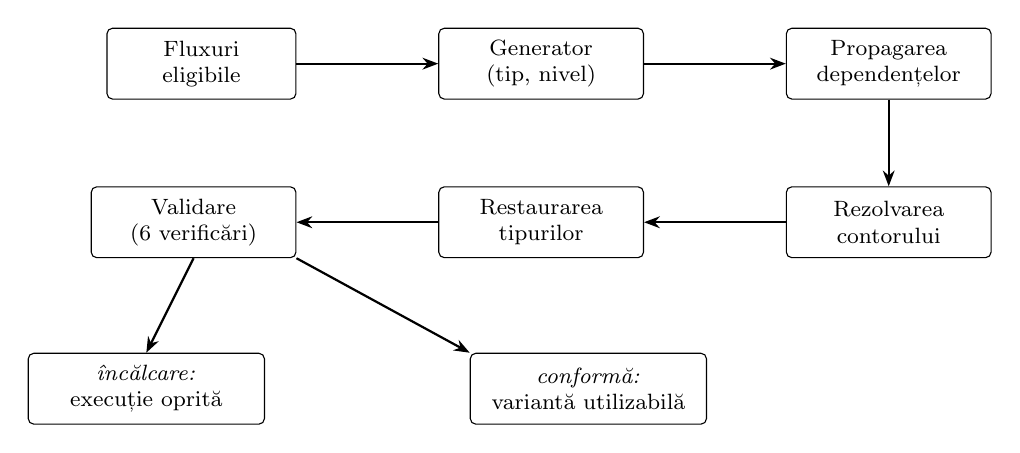
\begin{tikzpicture}[node distance=6mm and 18mm]
        \node[bloc, minimum width=24mm] (in) {Fluxuri\\ eligibile};
        \node[bloc, minimum width=26mm, right=of in] (gen) {Generator\\ (tip, nivel)};
        \node[bloc, minimum width=26mm, right=of gen] (prop) {Propagarea\\ dependențelor};
        \node[bloc, minimum width=26mm, below=11mm of prop] (ct) {Rezolvarea\\ contorului};
        \node[bloc, minimum width=26mm, left=of ct] (tip) {Restaurarea\\ tipurilor};
        \node[bloc, minimum width=26mm, left=of tip] (val) {Validare\\ (6 verificări)};
        \node[bloc, minimum width=30mm, below=12mm of val, xshift=-6mm] (stop) {\textit{încălcare:}\\ execuție oprită};
        \node[bloc, minimum width=30mm, below=12mm of tip, xshift=6mm] (ok) {\textit{conformă:}\\ variantă utilizabilă};

        \draw[sageata] (in) -- (gen);
        \draw[sageata] (gen) -- (prop);
        \draw[sageata] (prop) -- (ct);
        \draw[sageata] (ct) -- (tip);
        \draw[sageata] (tip) -- (val);
        \draw[sageata] (val.south) -- (stop.north);
        \draw[sageata] (val.south east) -- (ok.north west);
    \end{tikzpicture}
    \caption{Fluxul motorului de generare a variantelor perturbate. Validarea este ultima etapă înaintea utilizării: o variantă care încalcă o constrângere oprește execuția, în locul unei corecții tacite.}
    \label{fig:motor}
\end{figure}

Două decizii de proiectare necesită explicații suplimentare, deoarece verificările inițiale produceau rezultate aparent corecte, fără a evalua însă condițiile urmărite.

\textbf{Verificarea consistenței se face per rând, nu global.} În prima variantă, eroarea relativă a identităților algebraice era comparată cu o toleranță derivată din valoarea maximă a caracteristicii pe întregul set. Întrucât unele caracteristici au valori maxime de ordinul milioanelor, toleranța rezultată era atât de mare încât verificarea trecea indiferent de conținut. Formularea corectă compară eroarea fiecărui rând cu eroarea aceluiași rând în datele originale: cerința nu este ca identitatea să fie respectată exact, ea nu este respectată nici în datele brute, ci ca perturbarea să nu o degradeze suplimentar.

\textbf{Limitele de domeniu se aplică relativ la rândul original.} Formulate ca praguri absolute derivate din specificațiile protocoalelor, ele respingeau fluxuri prezente în captura reală: setul conține 61 de înregistrări cu valori TTL sub pragul de livrabilitate și o înregistrare a cărei dimensiune medie a pachetului depășește unitatea maximă de transmisie. Deoarece obiectul verificării este perturbarea, nu calitatea datelor de intrare, condiția corectă este ca varianta perturbată să nu încalce o limită mai grav decât o încălca deja rândul original.

Validatorul este supus unei \textbf{testări negative}: șapte variante construite în mod deliberat cu încălcări ale constrângerilor sunt introduse în sistem, cu cerința ca fiecare să fie respinsă. Acestea includ aplicarea umpluturii în sens invers, modificarea unei caracteristici asociate victimei, rescrierea unei caracteristici de identificare și introducerea unor valori nedefinite. Testarea confirmă astfel că validatorul identifică intrările nevalide, nu doar că se execută fără a produce erori.

\section{Măsurarea evaziunii}\label{sec:implmasurare}

Modulul de măsurare încarcă, pentru fiecare model, predicțiile de referință și masca de eligibilitate calculată conform criteriului din subsecțiunea~\ref{subsec:eligibil}, apoi aplică modelul fiecărei variante și clasifică rezultatele conform taxonomiei din subsecțiunea~\ref{subsec:rezultate}.

Variantele nu sunt citite de pe disc, ci regenerate în memorie la momentul măsurării, folosind aceleași generatoare. Generarea fiind deterministă, rezultatul este identic, iar spațiul de stocare necesar scade de la zeci de gigaocteți la câțiva megaocteți. Se persistă doar fișa rulării, rapoartele de validitate și eșantioane de câteva sute de rânduri per variantă, suficiente pentru inspecție manuală.

Pe lângă etichete, modulul înregistrează și distribuțiile de probabilitate, din care calculează deplasarea încrederii modelului: creșterea probabilității atribuite clasei traficului legitim și scăderea probabilității atribuite clasei reale. Aceste mărimi sunt informative chiar și acolo unde eticheta finală nu s-a modificat, deoarece arată cât de aproape de granița de decizie a fost împins fluxul.

Agregarea produce ratele per variantă, defalcarea per clasă de atac, cu marcarea explicită a claselor al căror suport este prea mic pentru o interpretare stabilă, intervalele definite în subsecțiunea~\ref{subsec:interval} pentru perechile de politici, și intensitatea minimă la care fiecare flux evadează pentru prima dată. Ultima mărime răspunde întrebării cât de mare trebuie să fie perturbarea, distinctă de întrebarea câte fluxuri evadează.

Înaintea oricărei agregări se verifică invariantul identității: rata de evaziune pe varianta identică trebuie să fie exact nulă pentru toate modelele. Verificarea este obligatorie și blochează execuția în caz de eșec. Măsurarea pe o singură variantă și încadrarea fiecărui flux în cele trei rezultate posibile sunt reproduse în secțiunile~\ref{sec:anexa-masurare} și \ref{sec:anexa-outcomes}.

\section{Analiza de sensibilitate}\label{sec:implsensibilitate}

Modulul măsoară cât contează fiecare caracteristică pentru decizia modelului, urmând procedura descrisă în subsecțiunea~\ref{subsec:agnostic}, cu cinci repetări pentru fiecare caracteristică, pe modelele înghețate. Metrica principală este scăderea ratei de detecție, din motivele de comensurabilitate expuse în subsecțiunea~\ref{subsec:comensurabil}. Se raportează suplimentar și scăderea de macro-$F1$. Bucla de permutare este reprodusă în secțiunea~\ref{sec:anexa-importanta-cod}.

Analiza restrânsă la o singură clasă de atac a necesitat o corecție de implementare. Permutarea uzuală amestecă valorile coloanei în interiorul eșantionului analizat. Dacă acest eșantion conține o singură clasă, iar caracteristica are aproape aceeași valoare pentru toate observațiile ei, amestecarea nu schimbă practic nimic, iar importanța măsurată apare fals ca fiind nulă, deși caracteristica poate fi tocmai cea pe care se sprijină decizia. Soluția implementată este substituția valorilor dintr-o distribuție \emph{donoare} externă, extrasă din întregul set de testare, care rupe efectiv legătura dintre caracteristică și etichetă.

Un al doilea modul pune în corespondență importanța cu evaziunea. Pentru fiecare transformare se însumează importanțele caracteristicilor pe care le afectează și se corelează seria rezultată cu ratele de evaziune corespunzătoare, prin coeficientul de corelație a rangurilor. Tot aici se calculează fracțiunea accesibilă definită de subsecțiunea~\ref{subsec:accesibila}, prin însumarea importanțelor pe categoriile din tabelul~\ref{tab:taxonomie}.

Un al treilea modul analizează destinațiile rezultatului de tip (c): pentru fiecare model se construiește distribuția claselor către care migrează fluxurile perturbate care rămân semnalate, și se compară profilul de încredere al fluxurilor care evadează cu al celor care nu evadează.

\section{Antrenarea adversarială}\label{sec:impladversarial}

Etapa de antrenare adversarială este singura care produce modele noi. Din acest motiv, ea respectă o regulă suplimentară față de celelalte: nu scrie niciodată în locațiile ocupate de modelele de referință și nici în artefactele derivate din ele. Modelele rezultate și rezultatele lor sunt păstrate în directoare separate, astfel încât toate măsurătorile anterioare rămân valabile și reproductibile după rulare.

\subsection{Reutilizarea mecanismului de perturbare}\label{subsec:reutilizare}

Cerința formulată pentru interfața interactivă în secțiunea~\ref{sec:implinterfata} se aplică identic aici, din același motiv: generatoarele nu sunt reimplementate, ci apelate. Datele de antrenare augmentate se obțin prin aceleași funcții care produc variantele măsurate, cu aceeași propagare a caracteristicilor derivate și aceeași restaurare a tipurilor. Dacă etapa aceasta ar fi construit propriile transformări, modelul ar fi fost antrenat pe o familie de perturbări ușor diferită de cea pe care este ulterior evaluat, iar rezultatul nu ar mai fi spus nimic despre robustețea la perturbările măsurate.

Diferă însă un singur parametru al apelului, cel discutat în subsecțiunea~\ref{subsec:provenienta}: contextul din care generatoarele își extrag statisticile auxiliare este construit exclusiv din partiția de antrenare. Funcția care construiește acest context înregistrează numărul de rânduri al fiecărui cadru sursă primit, iar etapa de augmentare verifică explicit, înainte de a genera orice, că a primit un singur cadru și că acesta are dimensiunea partiției de antrenare. Verificarea este o aserțiune care oprește execuția, nu un avertisment, pentru că scurgerea pe care o previne ar fi invizibilă în rezultate.

\subsection{Eșantionarea variantelor}\label{subsec:esantionare}

Fiecărui flux de atac care primește o copie i se atribuie o variantă prin extragere uniformă peste tipurile admise, urmată de o extragere uniformă peste nivelurile tipului ales. Tipurile marcate nerealizabile sunt excluse din start, la fel și cele scoase deliberat pentru grupul de generalizare.

Implementarea este vectorizată: se extrag simultan atribuirile tuturor rândurilor, apoi acestea se grupează pe perechi de tip și nivel, iar generatorul este apelat o singură dată pentru fiecare grup, pe sub-cadrul corespunzător. Alternativa evidentă, un apel per rând, ar fi fost inutilizabilă, generatoarele operează pe cadre întregi, iar costul fix al unui apel ar fi dominat complet. În forma grupată, augmentarea întregului set de atac durează sub o secundă, ceea ce face practicabilă reeșantionarea la fiecare epocă.

Ordinea rândurilor este fixată înaintea extragerii, iar generatorul de numere aleatoare este inițializat din perechea formată de \textit{seed}-ul rulării și numărul epocii. Varianta atribuită unui flux la o epocă dată se reproduce prin urmare exact, fără a depinde de ordinea în care sunt parcurse loturile sau de planificarea firelor de execuție. Alegerea de a extrage toate atribuirile înaintea construirii loturilor, în locul extragerii la momentul accesării fiecărei observații, este tocmai ceea ce face posibilă această garanție.

\subsection{Două regimuri de augmentare}\label{subsec:regimuri}

Cele două familii de modele primesc datele augmentate în moduri diferite, impuse de mecanismele lor de antrenare.

Ansamblurile de arbori sunt construite dintr-o singură trecere peste un set fix. Ele primesc, prin urmare, setul augmentat o singură dată, cu o variantă atribuită definitiv fiecărui flux de atac. Rețeaua neuronală parcurge însă zeci de treceri peste date, ceea ce permite ca aceleași fluxuri să apară la fiecare trecere cu o altă variantă. Figura~\ref{fig:augmentare} prezintă acest al doilea regim.

Al doilea regim este obținut prin trei metode scurte, apelate câte o dată pe
epocă:

\begin{verbatim}
def epoch_seed(self, epoch: int) -> int:
    """Seed-ul extragerii pentru o epoca."""
    return int(self.seed) * 1_000_003 + int(epoch)

def variants_for_epoch(self, epoch: int) -> pd.DataFrame:
    """Variantele atribuite randurilor de atac la epoca data."""
    frames = []
    for copy_index in range(self.k):
        frames.append(augment.assign_variants(
            len(self.attack_X),
            self.epoch_seed(epoch) + copy_index * 7919,
            self.holdout))
    return pd.concat(frames, ignore_index=True)

def loader_for_epoch(self, epoch: int):
    """DataLoader-ul epocii, amestecat determinist."""
    num, cat, y = self.tensors_for_epoch(epoch)
    return training.make_loader(num, cat, y,
                                config.TRANSFORMER_BATCH_SIZE,
                                shuffle=True,
                                seed=self.epoch_seed(epoch))
\end{verbatim}

Numărul epocii intră în \texttt{epoch\_seed} alături de \textit{seed}-ul rulării,
astfel încât fiecare epocă primește o extragere proprie, dar complet
reproductibilă. Aceeași valoare inițializează și amestecarea loturilor, deci
epoca se reface identic indiferent de ordinea în care sunt parcurse loturile
sau de planificarea firelor de execuție.

Metoda \texttt{loader\_for\_epoch} este singurul punct de legătură cu bucla de
antrenare: ea se transmite acesteia ca argument, iar bucla o apelează la
începutul fiecărei epoci în locul unui set fix. Regimul static se obține
transmițând în locul ei valoarea nulă, caz în care bucla folosește setul primit
o singură dată. Diferența dintre cele două regimuri se reduce, prin urmare, la
un singur argument, iar restul procedurii de antrenare rămâne neschimbat.

\begin{figure}[!ht]
    \centering
    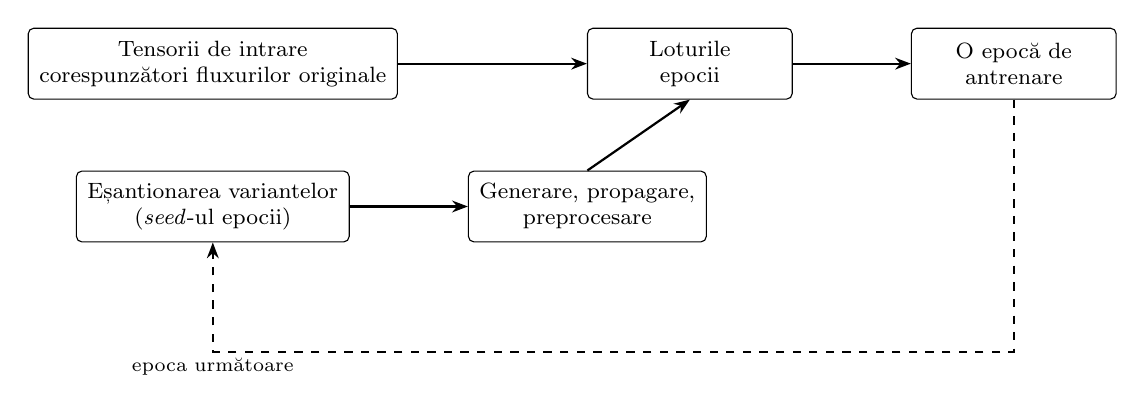
\begin{tikzpicture}[node distance=9mm and 15mm]
        \node[blocmare] (baza) {Tensorii de intrare\\ corespunzători fluxurilor originale};
        \node[blocmare, below=of baza] (esant) {Eșantionarea variantelor\\ (\textit{seed}-ul epocii)};
        \node[blocmare, right=of esant] (gen) {Generare, propagare,\\ preprocesare};
        \node[blocmare, right=24mm of baza] (lot) {Loturile\\ epocii};
        \node[bloc, right=of lot, minimum width=26mm] (ep) {O epocă de\\ antrenare};

        \draw[sageata] (baza) -- (lot);
        \draw[sageata] (esant) -- (gen);
        \draw[sageata] (gen.north) -- (lot.south);
        \draw[sageata] (lot) -- (ep);
        \draw[punctat] (ep.south) -- ++(0,-32mm) -|
            node[eticheta, pos=0.5, below] {epoca următoare} (esant.south);
    \end{tikzpicture}
\caption{Augmentarea dinamică folosită la antrenarea rețelei. Datele fluxurilor originale sunt preprocesate o singură dată, iar la fiecare epocă sunt reeșantionate variantele fluxurilor de atac și este regenerată partea perturbată a loturilor de antrenare.}    \label{fig:augmentare}
\end{figure}

Diferența are o consecință care trebuie raportată, nu ascunsă: rețeaua vede, pe parcursul antrenării, mai multe variante distincte ale aceluiași flux decât arborii. Tentația de a egaliza expunerea, mărind numărul de copii primite de arbori, a fost respinsă deliberat. Numărul de rânduri crește liniar cu acest număr, iar la valori care ar apropia expunerea arborilor de cea a rețelei proporția dintre trafic normal și trafic malițios s-ar deforma sever, iar memoria necesară construirii pădurii ar deveni ea însăși o constrângere. Soluția adoptată este menținerea unui număr mic și mărginit de copii pentru arbori și raportarea explicită a diferenței de expunere, comparația între cele două familii fiind tratată ca orientativă, nu ca paritate controlată.

\subsection{Transmiterea explicită a ponderilor de clasă}\label{subsec:implponderi}

Principiul enunțat în subsecțiunea~\ref{subsec:ponderi} se traduce diferit pentru fiecare model. Random Forest primește în mod obișnuit o indicație simbolică prin care își calculează singur ponderile din frecvențele setului primit. Aici, în locul indicației, i se transmite dicționarul de valori calculat pe setul original. Transformer primește vectorul corespunzător, ordonat conform codificării etichetelor. Modelul cu XGBoost nu folosește ponderi de clasă nici în varianta de referință, deci pentru el nu există nimic de fixat.

\begin{verbatim}
def balanced_weights(y_original) -> dict:
    """Ponderile calculate pe etichetele ORIGINALE."""
    classes = np.unique(np.asarray(y_original))
    values = compute_class_weight("balanced", classes=classes,
                                  y=np.asarray(y_original))
    return {cls: float(w) for cls, w in zip(classes, values)}


def build_rf(numeric_cols, class_weight: dict,
             seed: int) -> Pipeline:
    """class_weight primeste dictionarul inghetat in locul
    sirului "balanced", ca ponderile sa nu se recalculeze pe
    numaratorile augmentate.
    """
    return Pipeline([
        ("rare", RareCategoryGrouper(
            columns=config.CATEGORICAL_COLUMNS,
            min_freq=config.MIN_CATEGORY_FREQUENCY)),
        ("prep", build_preprocessor(numeric_cols)),
        ("clf", RandomForestClassifier(
            n_estimators=config.RF_N_ESTIMATORS,
            class_weight=class_weight,
            n_jobs=config.RF_N_JOBS,
            random_state=seed)),
    ])
\end{verbatim}

Toată diferența față de varianta de referință se află într-un singur argument.
Acolo unde modelul inițial primea șirul \texttt{"balanced"}, prin care
biblioteca își calcula singură ponderile din numărătorile setului primit, aici
primește dicționarul produs de \texttt{balanced\_weights} pe etichetele
originale. Restul componentelor rămân identice, ceea ce face verificabilă
afirmația că grupurile diferă doar prin date.

Ponderile nu sunt calculate o singură dată pentru toate modelele, ci o dată pentru fiecare familie, pe exact mulțimea de etichete pe care varianta de referință le-a calculat. Arborii sunt antrenați pe întreaga partiție de antrenare, iar Transformer pe sub-setul rămas după decuparea validării. Cele două mulțimi diferă, deci și ponderile diferă ușor. Folosirea unui singur vector pentru ambele ar fi introdus tocmai diferența de obiectiv pe care procedura urmărește să o elimine.

\subsection{Decuparea validării înaintea augmentării}\label{subsec:implsplit}

Pentru Transformer, împărțirea în sub-set de antrenare și set de validare se face pe rândurile originale, înaintea oricărei augmentări, cu același \textit{seed} și aceeași fracțiune ca la varianta de referință. Egalitatea cu împărțirea originală este verificată prin compararea mulțimilor de identificatori, nu presupusă.

Copiile perturbate se generează apoi exclusiv din rândurile aflate de partea de antrenare. O verificare separată confirmă că mulțimea identificatorilor sursă ai rândurilor generate este inclusă în cea a sub-setului de antrenare și disjunctă de cea a validării. Fără această condiție, o copie a unui flux de antrenare ar putea ajunge în validare, iar scorul care decide oprirea antrenării ar fi calculat parțial pe date derivate din antrenare.

Setul de validare rămâne integral nemodificat. Criteriul de selecție a modelului final este cel din varianta de referință, calculat pe trafic curat. Alegerea este deliberată și este argumentată în subsecțiunea~\ref{subsec:confuzii}: dacă oprirea ar fi condusă de un scor măsurat pe date perturbate, grupul apărat ar diferi de cel de referință atât prin date, cât și prin criteriul de selecție, iar comparația nu ar mai fi controlată. Robustețea se măsoară după antrenare, nu în timpul ei.

\subsection{Reluarea și artefactele de reproductibilitate}\label{subsec:implreluare}

Antrenarea rețelei de referință salvează periodic starea completă, inclusiv starea generatoarelor de numere aleatoare și pe cea a mecanismului care produce loturile, ceea ce permite reluarea exactă după o întrerupere. Pentru grupurile augmentate, mecanismul nu mai este suficient: loturile fiind regenerate la fiecare epocă, starea salvată nu descrie complet situația de reluat. Soluția adoptată este reluarea la granularitatea grupului: fiecare model deja salvat este sărit la o rulare ulterioară, iar o întrerupere costă cel mult grupul aflat în curs. Aceeași regulă se aplică și etapei de evaluare, unde fiecare rulare deja măsurată este sărită.

Seturile de date augmentate nu sunt salvate integral, deoarece pot fi reconstruite în mod determinist într-un timp redus. Persistarea celor patru seturi, fiecare conținând câteva sute de mii de rânduri, ar crește inutil necesarul de stocare și de memorie. Pentru fiecare set este salvată în schimb o amprentă criptografică, calculată după ordonarea coloanelor reprezentării tabelare. Aceasta permite verificarea faptului că datele reconstruite ulterior sunt identice cu cele utilizate inițial.

Pentru fiecare rulare este generată o fișă care înregistrează parametrii necesari reproducerii experimentului: \textit{seed}-ul folosit, numărul de copii generate pentru fiecare flux, variantele permise, probabilitățile de eșantionare pentru fiecare tip și variantă, ponderile utilizate, precum și compoziția și amprenta fiecărui set de date. Manifestul include, de asemenea, proveniența contextelor de generare, rezultatele verificărilor de integritate și pragurile stabilite pentru criteriile de evaluare. Valorile efectiv folosite sunt listate în secțiunea~\ref{sec:anexa-config}. Aceste praguri sunt înregistrate înainte de începerea rulării, conform procedurii descrise în subsecțiunea~\ref{subsec:preinregistrare}.

\subsection{Evaluarea pe mulțimea comună}\label{subsec:implcohorta}

Modulul de evaluare parcurge, pentru fiecare model antrenat, aceeași grilă de variante ca etapa de măsurare sistematică și înregistrează rezultatul fiecărui flux la fiecare variantă într-o matrice de coduri întregi pe un octet. Alegerea de a reține rezultatul tuturor fluxurilor de atac, nu doar al celor semnalate de modelul respectiv, este ceea ce permite recitirea aceleiași măsurători atât pe mulțimea proprie de fluxuri semnalate, cât și pe mulțimea comună definită în subsecțiunea~\ref{subsec:cohorta}, fără reluarea predicțiilor. Întreaga colecție de matrice ocupă câteva zeci de megaocteți.

Mulțimea comună se obține prin intersecția măștilor de eligibilitate ale tuturor rulărilor aceleiași familii de modele, citite din rândul corespunzător variantei identice al fiecărei matrice. Pe mulțimea astfel fixată se verifică din nou invariantul identității, iar apoi se calculează ratele globale, defalcarea per clasă de atac și mediile peste repetări.

Variantele pe care se face această măsurare sunt generate cu contextul complet, identic cu cel folosit la măsurarea sistematică, pentru ca perturbările evaluate să fie aceleași rând cu rând. Restricția la partiția de antrenare se aplică exclusiv generării datelor de antrenare. În momentul evaluării, modelele sunt deja antrenate și înghețate, deci nu mai pot fi influențate de proveniența statisticilor. Cele două roluri ale aceluiași mecanism sunt separate explicit în cod, prin două obiecte de context distincte, construite o singură dată și transmise mai departe.


\section{Interfața interactivă}\label{sec:implinterfata}

Interfața este realizată ca aplicație web locală și expune trei vederi: rezultatul agregat pe un grup de fluxuri, inspecția unui flux individual și tabelele și figurile măsurate sistematic.

Interfața nu își construiește propriile perturbări. Ea apelează exact aceleași funcții folosite la măsurarea sistematică, singura diferență fiind că valorile parametrilor vin de la utilizator, nu dintr-o listă stabilită dinainte. Cerința aceasta, formulată în secțiunea~\ref{sec:structura}, are un motiv practic. Dacă interfața ar avea propriul cod de perturbare, cele două implementări ar putea începe să difere după o modificare făcută doar în una dintre ele, iar cifrele afișate pe ecran nu ar mai corespunde celor raportate în lucrare.

Controalele sunt grupate într-un formular, astfel încât nicio recalculare să nu se producă până la acționarea butonului de rulare. Rațiunea este că valorile afișate trebuie să corespundă întotdeauna ultimei rulări, nu câmpurilor editate între timp. În absența acestei separări, un utilizator care modifică un parametru fără a-l aplica ar vedea rezultate care nu îi corespund. Parametrii efectiv utilizați sunt afișați într-un rezumat, tocmai pentru ca discrepanța dintre câmpurile editate și rezultatele afișate să fie explicită.

Modelele și datele se încarcă o singură dată și sunt păstrate în memorie între interacțiuni. Selecția fluxurilor dintr-o clasă se face prin eșantionare aleatoare cu \textit{seed} fix, nu prin preluarea primelor înregistrări: setul fiind ordonat după identificator, primele înregistrări nu sunt reprezentative pentru distribuția clasei, iar ratele afișate ar fi fost sistematic deplasate.

Dacă o combinație de parametri produce o variantă care încalcă o constrângere, interfața o semnalează explicit în locul afișării unui rezultat. Fără această verificare, utilizatorul ar putea obține o rată de evaziune ridicată pentru un flux imposibil fizic, iar valoarea ar fi lipsită de sens.

\section{Structurile de date persistate}\label{sec:structuri}

Comunicarea între etape se face exclusiv prin fișiere tabelare, ceea ce permite atât reluarea independentă a etapelor, cât și inspecția manuală a rezultatelor intermediare. Structurile principale sunt descrise în tabelul~\ref{tab:structuri}.

\begin{table}[H]
    \caption{Structurile de date schimbate între etape}
    \centering
    \begin{tabular}{|l|p{7.4cm}|}
        \hline
        \textbf{Structură} & \textbf{Conținut} \\
        \hline
        Predicții de referință & Identificator, etichetă reală și predicția fiecărui model pe traficul nemodificat \\
        \hline
        Distribuții de probabilitate & Matricea probabilităților per clasă, per model \\
        \hline
        Indicatori de eligibilitate & Masca definită în subsecțiunea~\ref{subsec:eligibil}, per model \\
        \hline
        Fișa variantelor & Câte o linie per variantă: tip, nivel, parametri, caracteristici modificate, statistici de rezolvare a contorului, cazuri degenerate, verificări executate și eșuate \\
        \hline
        Raportul de validitate & Câte o linie per verificare și per variantă, cu numărul de încălcări \\
        \hline
        Rezultate per flux & Identificator, etichetă reală, predicție și categorie de rezultat, pentru fiecare variantă și model \\
        \hline
        Agregări & Rate per variantă, defalcări per clasă, intervale, intensități minime \\
        \hline
    \end{tabular}
    \label{tab:structuri}
\end{table}

Fișa rulării are un rol care depășește evidența: el conține toate mărimile necesare pentru a stabili \emph{cât} din rezultatul unei variante depinde de decizii de rezervă. Numărul de rânduri rezolvate prin fiecare dintre cele trei niveluri descrise în subsecțiunea~\ref{subsec:ct} și numărul de cazuri degenerate din propagare sunt înregistrate explicit, astfel încât un rezultat obținut majoritar prin mecanisme de rezervă să poată fi identificat ca atare.

Rezultatele per flux sunt salvate comprimat, întrucât ele reprezintă produsul cartezian dintre fluxurile eligibile și variante. Ele sunt necesare analizei de sensibilitate, care compară profilul fluxurilor evadate cu al celor neevadate, comparație imposibilă pornind exclusiv de la agregări.

\section{Jurnalizarea și tratarea erorilor}\label{sec:jurnalizare}

Fiecare etapă produce un jurnal de execuție, scris simultan în consolă și într-un fișier din directorul de rezultate. Jurnalul înregistrează parametrii efectiv utilizați, dimensiunile datelor prelucrate, rezultatul fiecărei verificări și duratele etapelor intermediare.

Principiul adoptat în tratarea erorilor este eșecul explicit și timpuriu. O condiție încălcată oprește execuția cu un mesaj care indică verificarea și contextul, în locul continuării cu o valoare implicită. Alegerea este justificată de natura experimentală a codului: o etapă care continuă după o încălcare produce rezultate care par valide și care ar fi interpretate ca atare.

Continuarea procesului este condiționată de trecerea a trei verificări: validarea variantelor perturbate, concordanța dintre predicțiile modelului reîncărcat și cele ale modelului păstrat în memorie, precum și verificarea rezultatelor pentru varianta nemodificată. Dacă una dintre aceste verificări eșuează, etapele următoare nu mai sunt executate.


\section{Asigurarea reproductibilității}\label{sec:reproductibilitate}

Reproductibilitatea este esențială pentru interpretarea corectă a rezultatelor. Experimentele au fost executate în momente diferite, uneori la intervale de câteva săptămâni, astfel încât rezultatele pot fi comparate numai dacă repetarea unei rulări în aceleași condiții conduce la aceleași valori.

Pentru toate operațiile aleatoare este utilizată aceeași valoare inițială, definită în configurație. Aceasta este transmisă bibliotecilor folosite pentru prelucrarea datelor și antrenarea modelelor, inclusiv operațiilor executate pe placa grafică. În plus, inferența se desfășoară pe un singur fir de execuție, din motivele prezentate în subsecțiunea~\ref{subsec:inferenta}, iar pentru antrenarea rețelei sunt selectate operații deterministe, chiar dacă acestea presupun un timp de execuție mai mare.

La fiecare rulare completă se salvează un fișier cu hiperparametrii folosiți, versiunile bibliotecilor, ordinea caracteristicilor așteptată de model și un rezumat al setului de date. Utilitatea lui s-a văzut într-un caz concret. Instalarea unei biblioteci de analiză a coborât tacit versiunea unei dependențe numerice, iar rezultate deja obținute s-au schimbat. Fără versiunile înregistrate, diferența ar fi fost pusă pe seama unei modificări de cod și căutată acolo unde nu era.

Două verificări încheie această parte. Fiecare model salvat este reîncărcat de pe disc și pus să prezică din nou, iar predicțiile trebuie să coincidă cu cele obținute înainte de salvare. Apoi varianta neperturbată produsă de motorul de perturbare este trecută prin toate cele trei modele și trebuie să reproducă predicțiile de referință rând cu rând. Împreună cu invariantul identității, ele garantează că diferențele din capitolul următor provin din perturbări, nu din variații ale prelucrării.
 % \chapter{Proiectare de Detaliu și Implementare}

\chapter{Testare și validare}\label{ch:testare}
\pagestyle{fancy}

Capitolul prezintă rezultatele experimentale obținute și, înaintea lor, verificările care garantează că aceste rezultate măsoară ceea ce își propun să măsoare. Ordinea este deliberată: o rată de evaziune are sens doar dacă lanțul care a produs-o a fost validat în prealabil. Sunt raportate, în ordine, metodologia de testare, validarea lanțului de prelucrare, performanța clasificatoarelor pe trafic nemodificat, rezultatele măsurării evaziunii și analiza de sensibilitate.

\section{Metodologia de testare}\label{sec:metodologie}

\subsection{Mediul experimental}\label{subsec:mediu}

Experimentele au fost executate pe o singură configurație, cu versiuni fixate ale tuturor bibliotecilor, înregistrate automat la fiecare rulare în fișierul de metadate descris în secțiunea~\ref{sec:reproductibilitate}. Antrenarea rețelei neuronale a folosit accelerare grafică, iar restul etapelor se execută pe procesor.

Setul de date este utilizat în partiția oficială, fără reeșantionare și fără eliminarea vreunei observații. Partiția de testare conține 82\,332 de înregistrări, dintre care 45\,332 corespund traficului malițios. Toate măsurătorile adversariale se raportează exclusiv la aceste 45\,332 de fluxuri, filtrate ulterior prin criteriul de eligibilitate subsecțiunea~\ref{subsec:eligibil}.

\subsection{Nivelurile de verificare}\label{subsec:niveluri}

Testarea este organizată pe patru niveluri, fiecare adresând o clasă distinctă de erori:

\begin{enumerate}
    \item \textbf{Determinismul} (\textit{determinism}): aceeași intrare produce aceeași ieșire între rulări repetate.
    \item \textbf{Validitatea variantelor} (\textit{validity}): fiecare variantă perturbată respectă constrângerile din subsecțiunea~\ref{subsec:admisibile}.
    \item \textbf{Capacitatea de respingere} (\textit{negative testing}): suita de validare respinge efectiv variante invalide construite intenționat.
    \item \textbf{Invarianții de capăt la capăt} (\textit{end-to-end invariants}): varianta identică reproduce predicțiile de referință și produce evaziune nulă.
\end{enumerate}


\section{Caracterizarea setului de date}\label{sec:caracterizare}

\subsection{Distribuția claselor}\label{subsec:distributie}

Tabelul~\ref{tab:distributie} prezintă distribuția claselor în partiția de antrenare.

\begin{table}[!ht]
    \caption{Distribuția claselor în partiția de antrenare}
    \centering
    \begin{tabular}{|l|r|r|}
        \hline
        \textbf{Clasă} & \textbf{Observații} & \textbf{Pondere} \\
        \hline
        Normal & 56\,000 & 31,9\% \\
        \hline
        Generic & 40\,000 & 22,8\% \\
        \hline
        Exploits & 33\,393 & 19,0\% \\
        \hline
        Fuzzers & 18\,184 & 10,4\% \\
        \hline
        DoS & 12\,264 & 7,0\% \\
        \hline
        Reconnaissance & 10\,491 & 6,0\% \\
        \hline
        Analysis & 2\,000 & 1,1\% \\
        \hline
        Backdoor & 1\,746 & 1,0\% \\
        \hline
        Shellcode & 1\,133 & 0,6\% \\
        \hline
        Worms & 130 & 0,07\% \\
        \hline
    \end{tabular}
    \label{tab:distributie}
\end{table}

Raportul dintre clasa cea mai frecventă și cea mai rară este de \textbf{431 la 1}. Un asemenea dezechilibru confirmă inadecvarea acurateței globale ca indicator, discutată în secțiunea~\ref{sec:metrici}: un clasificator care ar prezice constant clasa majoritară ar obține o acuratețe de aproape $32\%$ fără nicio capacitate de discriminare, iar clasa cea mai rară ar putea fi ratată complet cu un cost neglijabil în acuratețe. Distribuția este reprezentată grafic, pe scară logaritmică, în figura~\ref{fig:distributie}.

\begin{figure}[!ht]
    \centering
    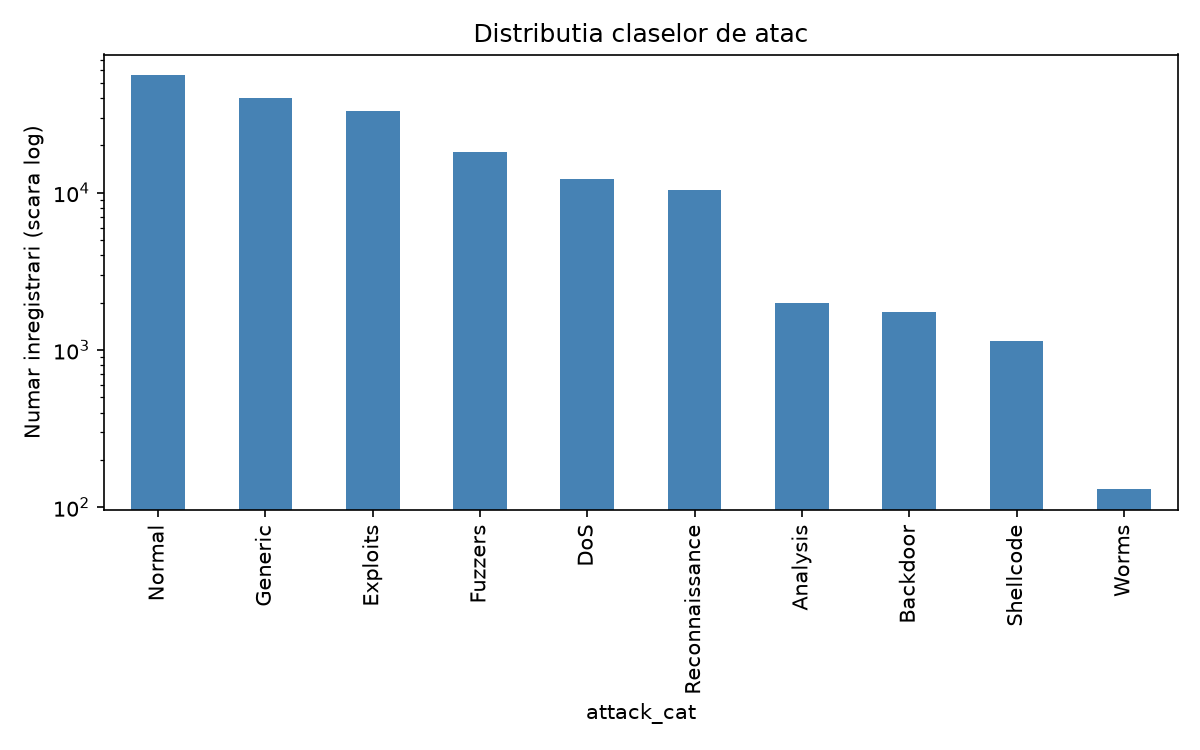
\includegraphics[width=0.85\textwidth]{figs/eda_class_distribution.png}
    \caption{Distribuția celor zece clase în partiția oficială de antrenare a setului UNSW-NB15, cele 175\,341 de fluxuri. Scara verticală este logaritmică, întrucât raportul dintre clasa cea mai frecventă și cea mai rară depășește $430{:}1$, iar pe scară liniară toate clasele rare ar fi indistinctibile de axă.}
    \label{fig:distributie}
\end{figure}

\subsection{Variabilele categorice}\label{subsec:categorice}

Analiza cardinalității variabilelor categorice a condus la două constatări cu efect direct asupra preprocesării.

Variabila care descrie protocolul are 133 de valori distincte, dintre care primele două acoperă împreună peste jumătate din observații, iar 118 apar de mai puțin de 200 de ori. La pragul de 50 de apariții folosit de mecanismul de grupare descris în subsecțiunea~\ref{subsec:rare}, doar trei protocoale sunt colapsate, ceea ce confirmă că reducerea dimensionalității nu este beneficiul principal al mecanismului în acest set.

Variabila care descrie starea conexiunii conține două valori prezente exclusiv în partiția de testare. Această situație justifică menținerea grupării: fără ea, valorile respective ar fi tratate tăcut, fără nicio urmă în raportare.

Variabila care descrie serviciul are o particularitate proprie: valoarea rezervată pentru serviciu necunoscut acoperă aproximativ 54\% din observații. Ea nu este, prin urmare, o categorie în sens obișnuit, ci un indicator de absență a informației.

\subsection{Caracteristicile numerice}\label{subsec:numerice}

Distribuțiile numerice sunt puternic asimetrice, cu coeficienți de asimetrie care ating valoarea 167 pentru adâncimea tranzacției și depășesc 39 pentru volumele de octeți și numărul de pachete. Asimetria justifică utilizarea scării logaritmice la reprezentarea grafică, dar nu impune nicio transformare în fluxul de modelare, din motivele expuse în subsecțiunea~\ref{subsec:eda}.

Analiza corelațiilor cu eticheta produce constatarea care se dovedește centrală pentru întreaga lucrare: valoarea TTL a pachetelor emise are coeficientul de corelație cel mai ridicat din întregul set, $0{,}693$, urmată de contorul de context asociat, cu $0{,}578$. Nicio altă caracteristică nu depășește valoarea $0{,}40$ în modul.

Primele două poziții sunt ocupate de o caracteristică asociată valorii TTL și de o caracteristică derivată din aceasta. Importanța lor ridicată sugerează încă din analiza exploratorie că modificarea acestor caracteristici poate influența predicțiile modelului, aspect evaluat ulterior în secțiunea~\ref{sec:rezultate-o3}. Verificarea setului de date nu a evidențiat valori lipsă, coloane cu varianță nulă sau înregistrări duplicate.


\section{Validarea lanțului de prelucrare}\label{sec:validare-lant}

\subsection{Verificarea determinismului}\label{subsec:det}

Instabilitatea predicției modelului Random Forest, descrisă în subsecțiunea~\ref{subsec:inferenta}, a fost măsurată direct înainte de corectare. Cinci apeluri identice de predicție pe același set de intrare au produs, față de o referință stocată, un număr de nepotriviri de $0, 1, 0, 1, 0$, variație mică în valoare absolută, dar nenulă și nedeterministă.

După impunerea execuției pe un singur fir, verificarea a fost repetată pe zece rulări consecutive, cu zero nepotriviri în toate cazurile. S-a confirmat totodată că predicțiile obținute în regim determinist coincid integral cu cele stocate anterior, ceea ce arată că măsura elimină variabilitatea fără a modifica vreun rezultat.

Au fost identificate 44 de fluxuri aflate în situația critică: 43 la egalitate exactă între primele două clase și unul cu o diferență la limita preciziei de reprezentare. Într-un set în care clasa cea mai rară are 44 de observații în partiția de testare, un asemenea număr de comutări posibile nu poate fi tratat ca zgomot.

\subsection{Validarea variantelor perturbate}\label{subsec:valvar}

Cele 28 de variante generate au fost supuse integral componentei de verificare din tabelul~\ref{tab:verificari}. Rezultatul este prezentat în tabelul~\ref{tab:validitate}.

\begin{table}[!ht]
    \caption{Rezultatul validării variantelor perturbate}
    \centering
    \begin{tabular}{|l|c|}
        \hline
        \textbf{Mărime} & \textbf{Valoare} \\
        \hline
        Fluxuri de atac prelucrate & 45\,332 \\
        \hline
        Variante generate & 28 \\
        \hline
        Verificări executate & 1\,259 \\
        \hline
        Verificări eșuate & \textbf{0} \\
        \hline
        Nepotriviri pe varianta identică & \textbf{0} \\
        \hline
    \end{tabular}
    \label{tab:validitate}
\end{table}

Creșterea maximă a erorii relative a identităților algebraice, măsurată per rând pe toate cele 28 de variante, a fost de ordinul $10^{-15}$, adică la nivelul preciziei de reprezentare în virgulă mobilă. Propagarea prin rapoarte, enunțată în subsecțiunea~\ref{subsec:propagare}, se comportă, prin urmare, exact conform predicției teoretice: ea nu degradează consistența internă a vectorului.

\subsection{Testarea negativă a suitei de validare}\label{subsec:negativ}

Pentru a demonstra că suita este capabilă să respingă, au fost construite șapte variante deliberat invalide, fiecare încălcând o singură constrângere. Rezultatele sunt prezentate în tabelul~\ref{tab:negativ}.

\begin{table}[!ht]
    \caption{Testarea negativă: variante invalide construite intenționat}
    \centering
    \begin{tabular}{|p{6.4cm}|l|}
        \hline
        \textbf{Încălcare introdusă} & \textbf{Rezultat} \\
        \hline
        Umplutură aplicată în sens invers & Respinsă \\
        \hline
        Durată redusă în loc de dilatată & Respinsă \\
        \hline
        Contor de conexiuni crescut & Respinsă \\
        \hline
        Coloană generată de victimă modificată & Respinsă \\
        \hline
        Caracteristică identitară rescrisă & Respinsă \\
        \hline
        Valoare nedefinită injectată prin propagare & Respinsă \\
        \hline
        Schemă alterată (tip de dată modificat) & Respinsă \\
        \hline
    \end{tabular}
    \label{tab:negativ}
\end{table}

Toate cele șapte variante au fost respinse, fiecare de verificarea corespunzătoare încălcării introduse. Rezultatul confirmă că cele 1\,259 de verificări trecute din tabelul~\ref{tab:validitate} constituie o dovadă de validitate, nu doar o execuție fără eroare.

Această etapă a avut și un rol corectiv. În versiunile intermediare, două verificări treceau din motive greșite: cea de consistență a dependențelor, din cauza unei toleranțe calculate global, și cea de limite de domeniu, din cauza unor praguri absolute. Ambele au fost descoperite exclusiv prin testare negativă și au fost reformulate conform discuției din subsecțiunea~\ref{subsec:validare}.

\subsection{Verificarea variantei nemodificate}
\label{subsec:invidentitate}

Varianta de nivel zero nu modifică valorile fluxurilor, dar trece prin toate etapele procesului de evaluare: generare, propagare, restabilirea tipurilor de date, validare și predicție. Scopul acestei verificări este de a determina dacă prelucrarea datelor produce modificări neintenționate.

Predicțiile obținute după prelucrare au fost comparate cu cele calculate direct pe fluxurile originale. Verificarea a fost realizată pentru toate cele trei modele și pentru cele 45\,332 de fluxuri de atac. Nu a fost identificată nicio diferență între predicții.

Rezultatul arată că trecerea datelor prin procesul de evaluare nu modifică predicțiile atunci când perturbarea este nulă. Verificarea poate evidenția erori precum schimbarea ordinii caracteristicilor, conversia incorectă a tipurilor de date sau actualizarea necorespunzătoare a caracteristicilor derivate.

\subsection{Verificarea montajului de antrenare adversarială}\label{subsec:val-adversarial}

Etapa de antrenare adversarială este singura care produce modele noi. Din acest motiv, este și singura care ar putea introduce o abatere față de rezultatele deja măsurate fără ca aceasta să se vadă în cifrele finale. Înainte de a interpreta vreun rezultat, au fost verificate separat elementele de mai jos.

\textbf{Reproducerea modelelor de referință.} Grupul antrenat pe datele originale ar trebui să fie identic cu modelul înghețat din capitolul anterior, primind exact aceleași date și aceiași hiperparametri. Există totuși o diferență de formă: ponderile de clasă îi sunt date ca listă explicită de valori, în locul cuvântului-cheie prin care biblioteca le calcula singură din numărătorile setului primit. Schimbarea era necesară pentru grupurile augmentate, unde numărătorile diferă, dar trebuia arătat că pe datele originale nu schimbă nimic. Altfel, chiar grupul de referință ar fi fost altul decât modelul înghețat, iar abaterea s-ar fi transmis tăcut tuturor comparațiilor. Comparația s-a făcut rând cu rând, pe întreaga partiție de testare, iar rezultatele sunt prezentate în tabelul~\ref{tab:reproducere}.

\begin{table}[!ht]
    \caption{Reproducerea modelelor înghețate de către grupul de referință}
    \centering
    \begin{tabular}{|l|c|c|}
        \hline
        \textbf{Model} & \textbf{Rânduri comparate} & \textbf{Nepotriviri} \\
        \hline
        Random Forest & 82\,332 & \textbf{0} \\
        \hline
        XGBoost & 82\,332 & \textbf{0} \\
        \hline
        Transformer & 82\,332 & \textbf{0} \\
        \hline
    \end{tabular}
    \label{tab:reproducere}
\end{table}

Pentru Transformer, egalitatea este mai puternică decât o simplă coincidență a predicțiilor finale: valorile funcției de cost și scorurile de validare ale primelor epoci coincid până la a patra zecimală cu cele înregistrate la antrenarea modelului de referință, ceea ce arată că traiectoria de optimizare este identică, nu doar punctul ei final. Rezultatul confirmă că fixarea ponderilor este, pe datele originale, o operație neutră, deci orice diferență observată la celelalte grupuri provine din date.

\textbf{Reproducerea lanțului de măsurare.} Modulul de evaluare al acestei etape parcurge grila de variante printr-un drum de cod propriu, distinct de cel folosit la măsurarea sistematică din secțiunea~\ref{sec:rezultate-o3}. Pentru a exclude o divergență între cele două, modelele înghețate au fost trecute prin noul drum și ratele obținute au fost comparate cu cele deja raportate. Pentru XGBoost, toate cele 28 de variante au coincis exact, cu o diferență absolută maximă de $0{,}0000$ puncte procentuale, iar numărul de fluxuri semnalate a fost identic, 44\,258. Măsurătorile noi sunt, prin urmare, direct comparabile cu cele anterioare.

\textbf{Proveniența statisticilor de generare.} Restricția din subsecțiunea~\ref{subsec:provenienta} a fost verificată prin numărul de combinații din tabelul de corespondențe al contorului de context: contextul construit pe ambele partiții conține 58 de combinații, iar cel construit exclusiv pe partiția de antrenare, 32. Diferența confirmă că restricția este efectivă, nu declarativă. Consecința practică este că generatorul recurge mai des la valorile de rezervă atunci când produce date de antrenare, ceea ce este raportat în fișa rulării.

\textbf{Compoziția seturilor augmentate.} Cu 175\,341 de rânduri în partiția de antrenare, dintre care 119\,341 de atac, adăugarea unei copii per flux malițios produce 294\,682 de rânduri, adică un factor de $1{,}68$, nu de $2$. Raportul dintre traficul de atac și cel normal crește de la $2{,}13$ la $4{,}26$. Grupul de control are, prin construcție, exact aceleași valori: aceeași dimensiune, aceleași numărătoare per clasă, aceeași proporție. Amprentele criptografice ale celor două seturi diferă, ceea ce confirmă că diferă efectiv prin conținut, nu doar prin etichetă.

\textbf{Împărțirea și apartenența la aceeași parte.} Împărțirea în sub-set de antrenare și set de validare coincide, la nivel de identificator, cu cea folosită la antrenarea modelului de referință. Verificarea de apartenență a confirmat că toți cei 149\,039 de identificatori sursă ai rândurilor generate provin din sub-setul de antrenare, niciunul din setul de validare.


\section{Performanța clasificatoarelor pe trafic nemodificat}\label{sec:rezultate-o1}

\subsection{Performanța globală}\label{subsec:global}

Tabelul~\ref{tab:metrici} prezintă rezultatele celor trei modele pe partiția oficială de testare.

\begin{table}[!ht]
    \caption{Performanța modelelor pe traficul nemodificat}
    \centering
    \begin{tabular}{|l|c|c|c|c|}
        \hline
        \textbf{Model} & \textbf{Acuratețe} & \textbf{Acuratețe ech.} & \textbf{Macro-$F1$} & \textbf{$F1$ ponderat} \\
        \hline
        Random Forest & 0,6913 & 0,5944 & 0,5010 & 0,7416 \\
        \hline
        XGBoost & \textbf{0,7659} & 0,5443 & \textbf{0,5098} & \textbf{0,7816} \\
        \hline
        Transformer & 0,6594 & \textbf{0,6288} & 0,4354 & 0,7168 \\
        \hline
    \end{tabular}
    \label{tab:metrici}
\end{table}

Ordinea modelelor depinde de metrica aleasă, ceea ce confirmă necesitatea raportării mai multor indicatori. Modelul cu XGBoost conduce la acuratețe, macro-$F1$ și $F1$ ponderat, în timp ce Transformer obține cea mai bună acuratețe echilibrată, adică cel mai bun comportament mediu pe clase, dar cel mai slab macro-$F1$. Diferența provine din faptul că acuratețea echilibrată mediază sensibilitățile, în timp ce macro-$F1$ penalizează și precizia scăzută: Transformer identifică o proporție mai mare din observațiile claselor rare, dar cu multe alarme false pe acele clase.

Poziția a treia a rețelei la macro-$F1$ nu constituie un eșec, ci rezultatul așteptat. Pe date tabelare, ansamblurile de arbori sunt frecvent competitive sau superioare arhitecturilor neuronale, iar obiectivul comparației, formulat în subsecțiunea~\ref{subsec:comparatie}, nu este stabilirea celui mai performant model, ci observarea comportamentului sub perturbări al unor modele cu predispoziții inductive diferite.

\subsection{Analiza per clasă}\label{subsec:perclasa}

Tabelul~\ref{tab:perclasa} prezintă scorul $F1$ pe fiecare clasă, împreună cu suportul acesteia în partiția de testare.

\begin{table}[!ht]
    \caption{Scorul $F1$ pe clase și suportul acestora în partiția de testare}
    \centering
    \begin{tabular}{|l|r|c|c|c|}
        \hline
        \textbf{Clasă} & \textbf{Suport} & \textbf{RF} & \textbf{XGB} & \textbf{Transformer} \\
        \hline
        Generic & 18\,871 & 0,981 & 0,985 & 0,981 \\
        \hline
        Normal & 37\,000 & 0,766 & 0,847 & 0,738 \\
        \hline
        Reconnaissance & 3\,496 & 0,849 & 0,866 & 0,757 \\
        \hline
        Exploits & 11\,132 & 0,699 & 0,711 & 0,645 \\
        \hline
        Worms & 44 & 0,593 & 0,500 & 0,241 \\
        \hline
        Shellcode & 378 & 0,399 & 0,495 & 0,267 \\
        \hline
        Fuzzers & 6\,062 & 0,376 & 0,396 & 0,355 \\
        \hline
        DoS & 4\,089 & 0,226 & 0,198 & \textbf{0,250} \\
        \hline
        Backdoor & 583 & 0,097 & 0,039 & \textbf{0,116} \\
        \hline
        Analysis & 677 & 0,025 & 0,062 & 0,003 \\
        \hline
    \end{tabular}
    \label{tab:perclasa}
\end{table}

Distribuția scorurilor este puternic neuniformă și se corelează doar parțial cu suportul. Clasa \textit{Generic} este recunoscută aproape perfect de toate modelele, în timp ce clasa \textit{Analysis}, cu un suport comparabil cu al altor clase rezonabil clasificate, este practic ratată de toate trei. Explicația nu este statistică, ci structurală: clasele \textit{Analysis} și \textit{Backdoor} se suprapun aproape complet în spațiul caracteristicilor, iar modelele nu dispun de informația necesară pentru a le separa.

Se observă totodată că Transformer obține cele mai bune scoruri pe \textit{DoS} și \textit{Backdoor}, adică exact pe două dintre clasele cele mai dificile, dar se prăbușește complet pe \textit{Analysis}. Comportamentul este consistent cu acuratețea echilibrată superioară din tabelul~\ref{tab:metrici}.

Matricele de confuzie confirmă interpretarea structurală. Cea a modelului XGBoost este prezentată în figura~\ref{fig:cm-xgb}, iar cea a modelului Random Forest în figura~\ref{fig:cm-rf}. În ambele cazuri, erorile nu sunt distribuite uniform, ci concentrate în blocuri corespunzătoare grupurilor de clase confundabile, ceea ce arată că modelele nu greșesc aleator, ci sistematic, între categorii care se suprapun în spațiul caracteristicilor.

\begin{figure}[!ht]
    \centering
    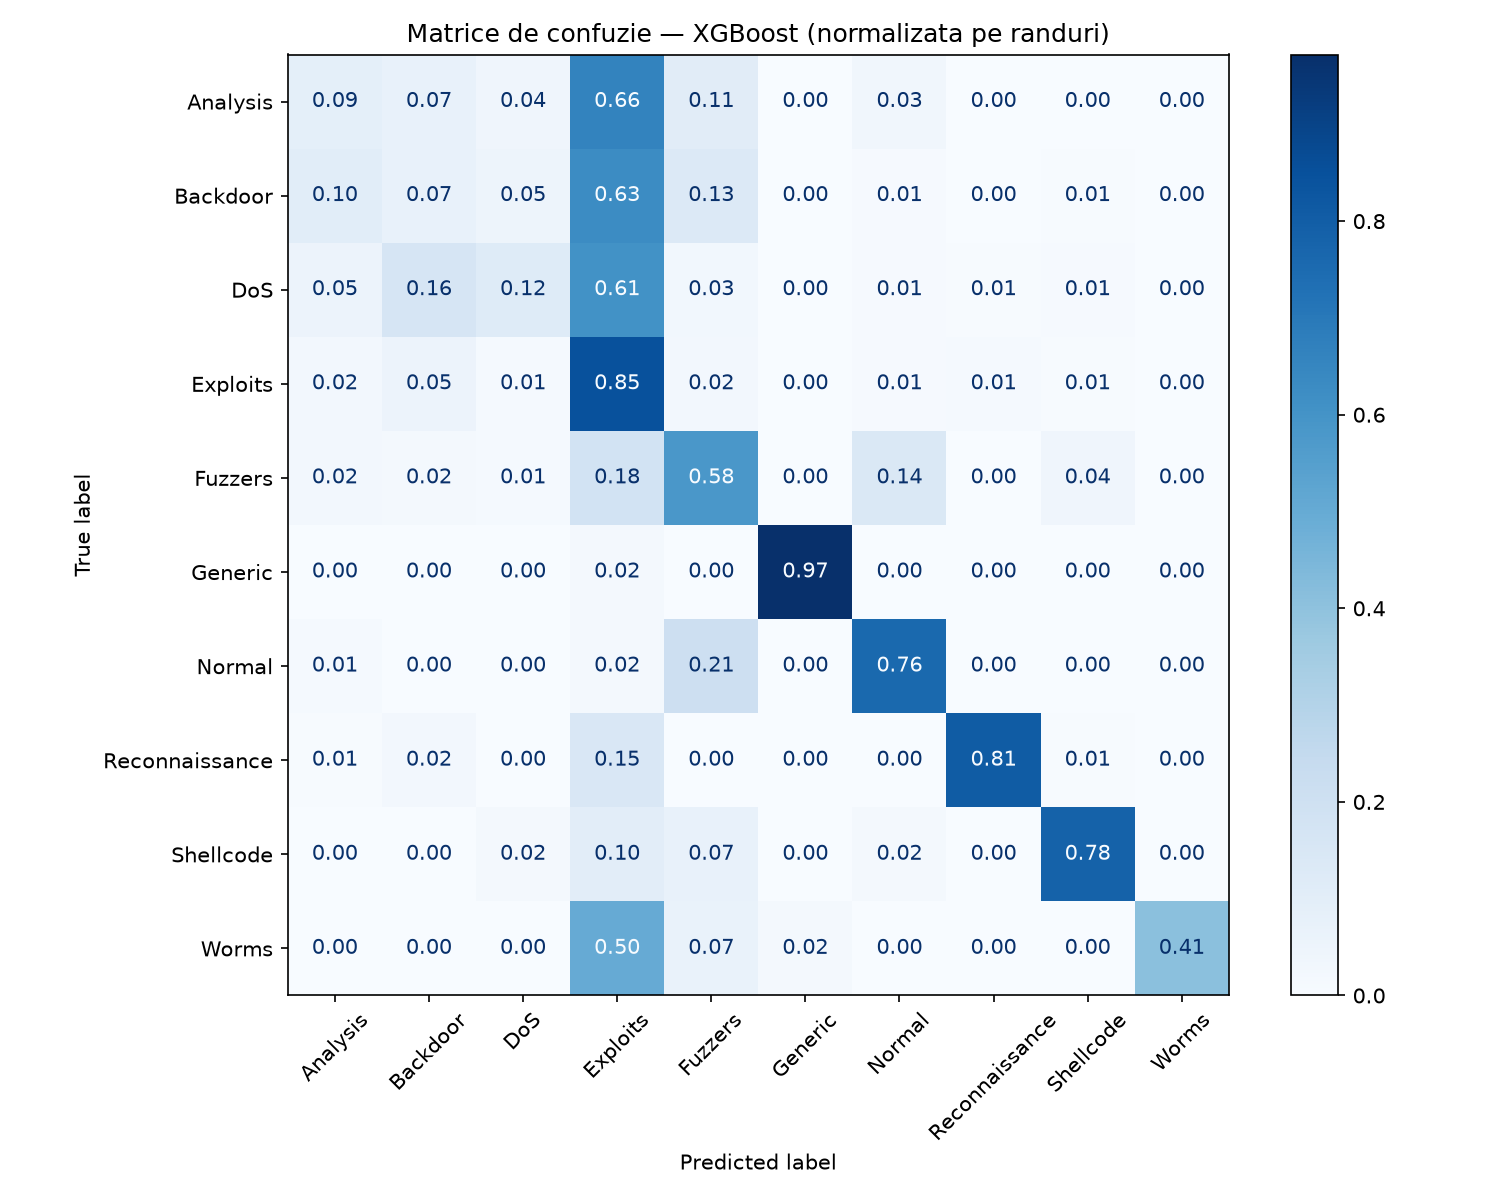
\includegraphics[width=0.80\textwidth]{figs/confusion_matrix_xgboost.png}
    \caption{Matricea de confuzie a modelului XGBoost}
    \label{fig:cm-xgb}
\end{figure}

\begin{figure}[!ht]
    \centering
    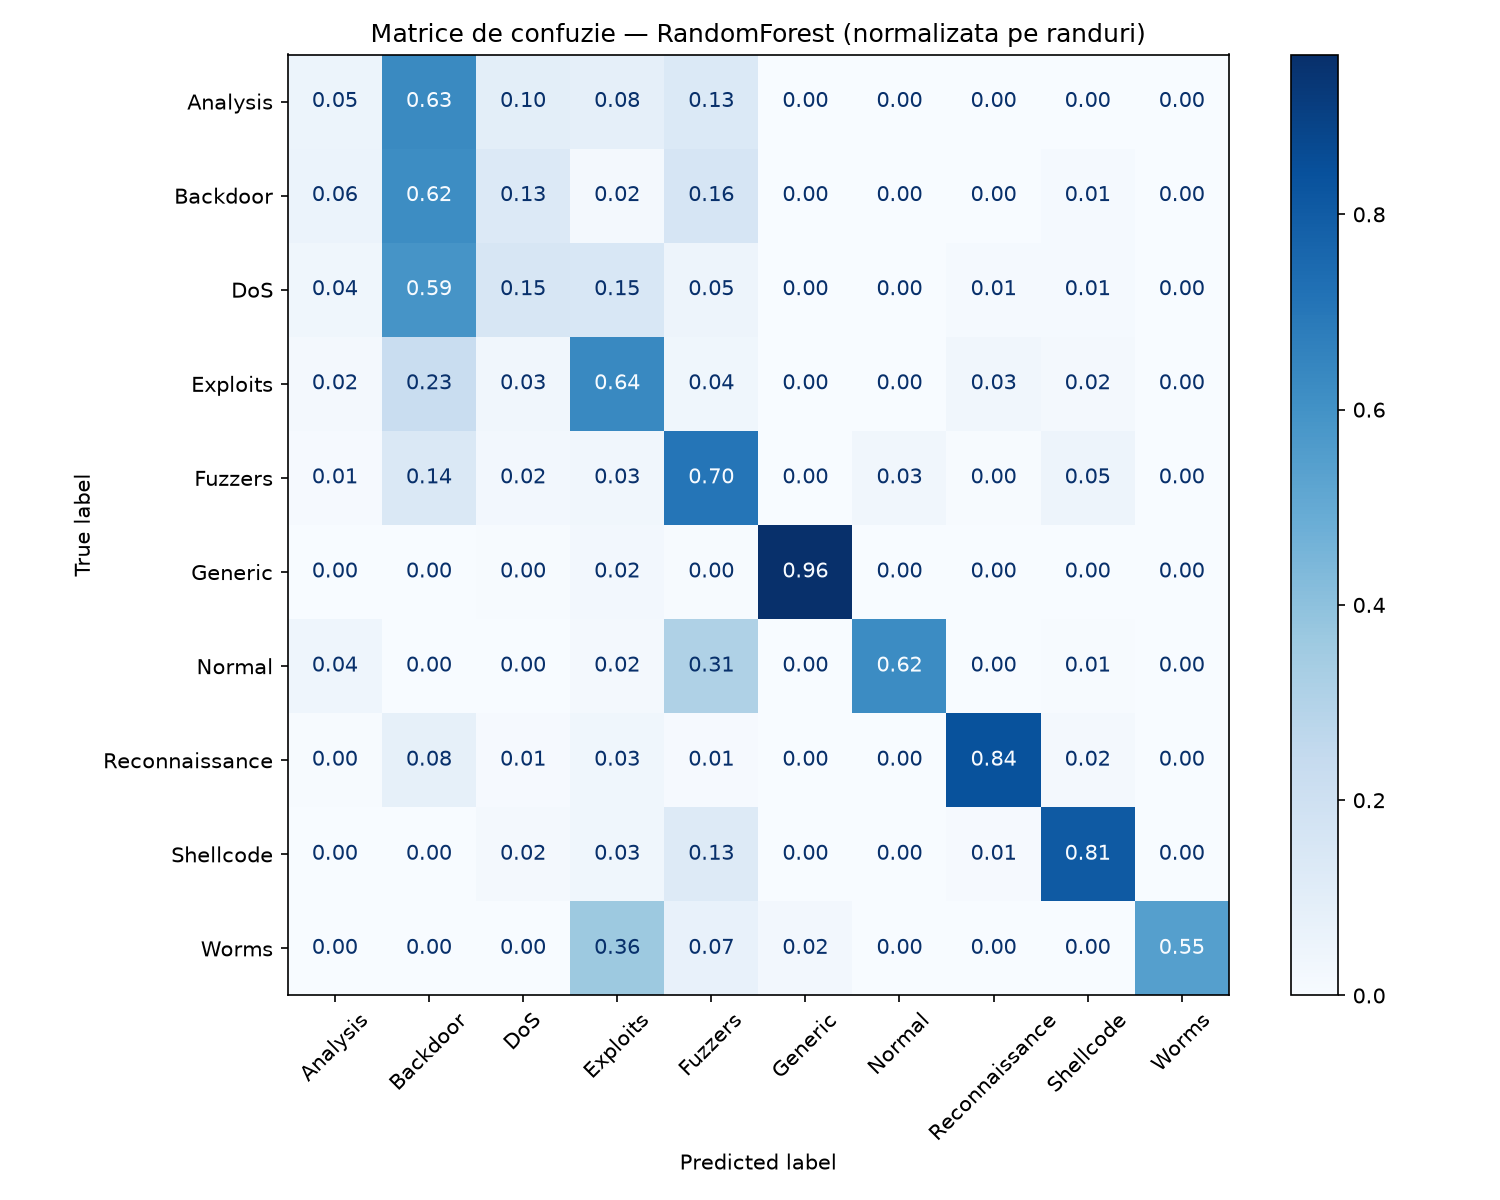
\includegraphics[width=0.80\textwidth]{figs/confusion_matrix_randomforest.png}
    \caption{Matricea de confuzie a modelului Random Forest}
    \label{fig:cm-rf}
\end{figure}

Se observă în ambele matrice că un număr important de fluxuri de atac sunt încadrate în categorii de atac greșite, dar foarte puține sunt clasificate drept trafic legitim. Această asimetrie este exact fenomenul cuantificat în subsecțiunea~\ref{subsec:semnalare}.

\subsection{Capacitatea de semnalare față de acuratețea subtipului}\label{subsec:semnalare}

Rezultatul cel mai important al acestei etape nu apare în tabelul~\ref{tab:metrici}. Deși macro-$F1$ se situează în jurul valorii de $0{,}50$, ceea ce ar sugera o capacitate de detecție modestă, aproape fiecare flux de atac declanșează o alarmă. Decalajul dintre cele două mărimi este prezentat în tabelul~\ref{tab:eligibil}, împreună cu prețul plătit pentru el pe traficul legitim.

\begin{table}[H]
    \caption{Cele două fețe ale detecției pe trafic nemodificat. Primele două coloane se referă la cele 45\,332 de fluxuri de atac, ultima la cele 37\,000 de fluxuri legitime.}
    \centering
    \begin{tabular}{|l|r|r|r|}
        \hline
        \textbf{Model} & \textbf{Clasificate corect} & \textbf{Alarmă declanșată} & \textbf{Alarme false} \\
        \hline
        Random Forest & 33\,812 \;(74,6\%) & \textbf{45\,116 \;(99,52\%)} & 13\,893 \;(37,5\%) \\
        \hline
        XGBoost & 35\,085 \;(77,4\%) & \textbf{44\,258 \;(97,63\%)} & 9\,029 \;(24,4\%) \\
        \hline
        Transformer & 32\,617 \;(72,0\%) & \textbf{45\,304 \;(99,94\%)} & 15\,326 \;(41,4\%) \\
        \hline
    \end{tabular}
    \label{tab:eligibil}
\end{table}

Distanța dintre primele două coloane este substanțială la toate trei modelele: 11\,304 fluxuri la Random Forest, 9\,173 la XGBoost și 12\,687 la Transformer sunt semnalate ca malițioase fără a fi încadrate în categoria corectă. Modelele greșesc mult mai des \emph{care} atac este decât \emph{dacă} este un atac.

A treia coloană arată însă că rata ridicată de semnalare nu trebuie citită ca o performanță de detecție. Modelele semnalează aproape toate atacurile și pentru că semnalează mult prea des în general: între un sfert și peste patru zecimi din traficul legitim primește alarmă. Matricea de confuzie din figura~\ref{fig:cm-rf} arată sursa principală, aproape o treime din traficul legitim fiind încadrat de Random Forest în clasa \textit{Fuzzers}. Un sistem cu acest profil ar fi greu de folosit în practică, unde volumul traficului legitim depășește cu ordine de mărime traficul de atac.

Nivelul acestor rate trebuie însă raportat la partiția pe care sunt măsurate. Partiția oficială UNSW-NB15 este dificilă tocmai pentru că cele două jumătăți ale ei nu provin din aceeași distribuție. Proporția traficului legitim crește de la $31{,}9\%$ la antrenare la $44{,}9\%$ la testare, iar în interiorul clasei legitime ponderea fluxurilor care poartă valoarea TTL 254, cea caracteristică atacurilor, se dublează, de la $20{,}1\%$ la $40{,}7\%$. La testare, modelele întâlnesc prin urmare de două ori mai mult trafic legitim purtând exact semnătura pe care au învățat-o ca indiciu de atac, ceea ce explică direct nivelul alarmelor false. Constatarea nu justifică valorile, dar arată că ele reflectă în bună măsură o proprietate a partiției, nu doar o alegere de model. Ele nu ar trebui, prin urmare, extrapolate ca rate de fals pozitiv ale acestor modele în general.

Constatarea are două consecințe. Prima este că definiția mulțimii eligibile din subsecțiunea~\ref{subsec:eligibil} nu este o convenție lipsită de efect: cele două criterii posibile diferă cu aproape un sfert din observații, iar alegerea între ele modifică numitorul tuturor ratelor raportate ulterior. A doua este că evaziunea devine o măsurătoare netrivială: dacă modelele ar rata deja o fracțiune importantă din atacuri, o rată de evaziune ridicată nu ar demonstra nimic despre efectul perturbării. Punctul de plecare fiind o semnalare cvasicompletă a atacurilor, orice creștere a evaziunii este atribuibilă perturbării. Argumentul se sprijină exclusiv pe coloana a doua din tabel și rămâne valabil indiferent de numărul alarmelor false, întrucât acestea privesc fluxuri legitime, care nu intră în măsurătoare.

\section{Antrenarea modelului Transformer}\label{sec:rezultate-transformer}

Antrenarea a parcurs 44 de epoci înainte de oprirea timpurie, cu selecția modelului la epoca 34 conform criteriului netezit descris în subsecțiunea~\ref{subsec:retea}. Curba scorului de validare a crescut rapid în primele epoci, după care a oscilat în jurul unui platou, ceea ce indică o convergență reală, nu un buget de antrenare insuficient.

Necesitatea criteriului netezit a fost confirmată empiric. Selecția pe valoarea instantanee a scorului de validare indica drept optim un maxim izolat, situat cu peste două abateri standard deasupra mediei locale a traiectoriei și urmat imediat de o revenire la nivelul anterior, adică semnătura tipică a unei fluctuații, nu a unui optim. Criteriul netezit, aplicat pe o fereastră de trei epoci, selectează în schimb un punct dintr-o regiune stabilă.

Este de subliniat că trecerea la criteriul netezit \emph{nu} a îmbunătățit scorul final: macro-$F1$ a scăzut ușor față de selecția pe valoarea instantanee, cu o diferență inferioară amplitudinii oscilațiilor de la o epocă la alta, ceea ce face cele două variante indistinctibile statistic. Justificarea păstrării criteriului netezit este metodologică, nu numerică: modelul reținut este reprezentativ pentru o regiune stabilă a traiectoriei, ceea ce constituie cerința corectă pentru un model destinat unor experimente ulterioare.

\section{Măsurarea ratei de evaziune}\label{sec:rezultate-o3}

\subsection{Rezultatul principal}\label{subsec:principal}

Tabelul~\ref{tab:evaziune} prezintă ratele de evaziune la intensitatea maximă a fiecărui tip de transformare realizabilă. Pentru transformările care implică valori TTL, rezultatul este raportat ca interval, conform discuției din subsecțiunea~\ref{subsec:interval}.

\begin{table}[!ht]
    \caption{Rate de evaziune la intensitate maximă (\% din fluxurile eligibile)}
    \centering
    \begin{tabular}{|l|c|c|c|}
        \hline
        \textbf{Transformare} & \textbf{RF} & \textbf{XGB} & \textbf{Transformer} \\
        \hline
        TTL & 4,4 -- 18,4 & \textbf{50,2 -- 51,1} & 4,0 -- 43,2 \\
        \hline
        Combinată & 31,3 -- 75,9 & \textbf{96,4 -- 96,9} & 17,4 -- 71,0 \\
        \hline
        Umplutură & 0,15 & 1,23 & 0,10 \\
        \hline
        Temporizare & 0,73 & 1,12 & 0,02 \\
        \hline
        Rată conexiuni & 0,33 & 0,56 & 0,00 \\
        \hline
    \end{tabular}
    \label{tab:evaziune}
\end{table}

\medskip
Rezultatul central este net: \textbf{modificarea TTL este singurul vector de perturbare care contează}. Umplutura, dilatarea temporală și reducerea ratei de conexiuni lasă rata de evaziune sub $1{,}3\%$ la orice intensitate și pentru orice model, în timp ce o singură modificare a valorii TTL duce XGBoost de la $0\%$ la peste $50\%$. Combinată cu celelalte transformări, aceeași modificare împinge rata la aproape $97\%$.

Evoluția pe niveluri de intensitate este prezentată în figura~\ref{fig:curbe}.

\begin{figure}[H]
    \centering
    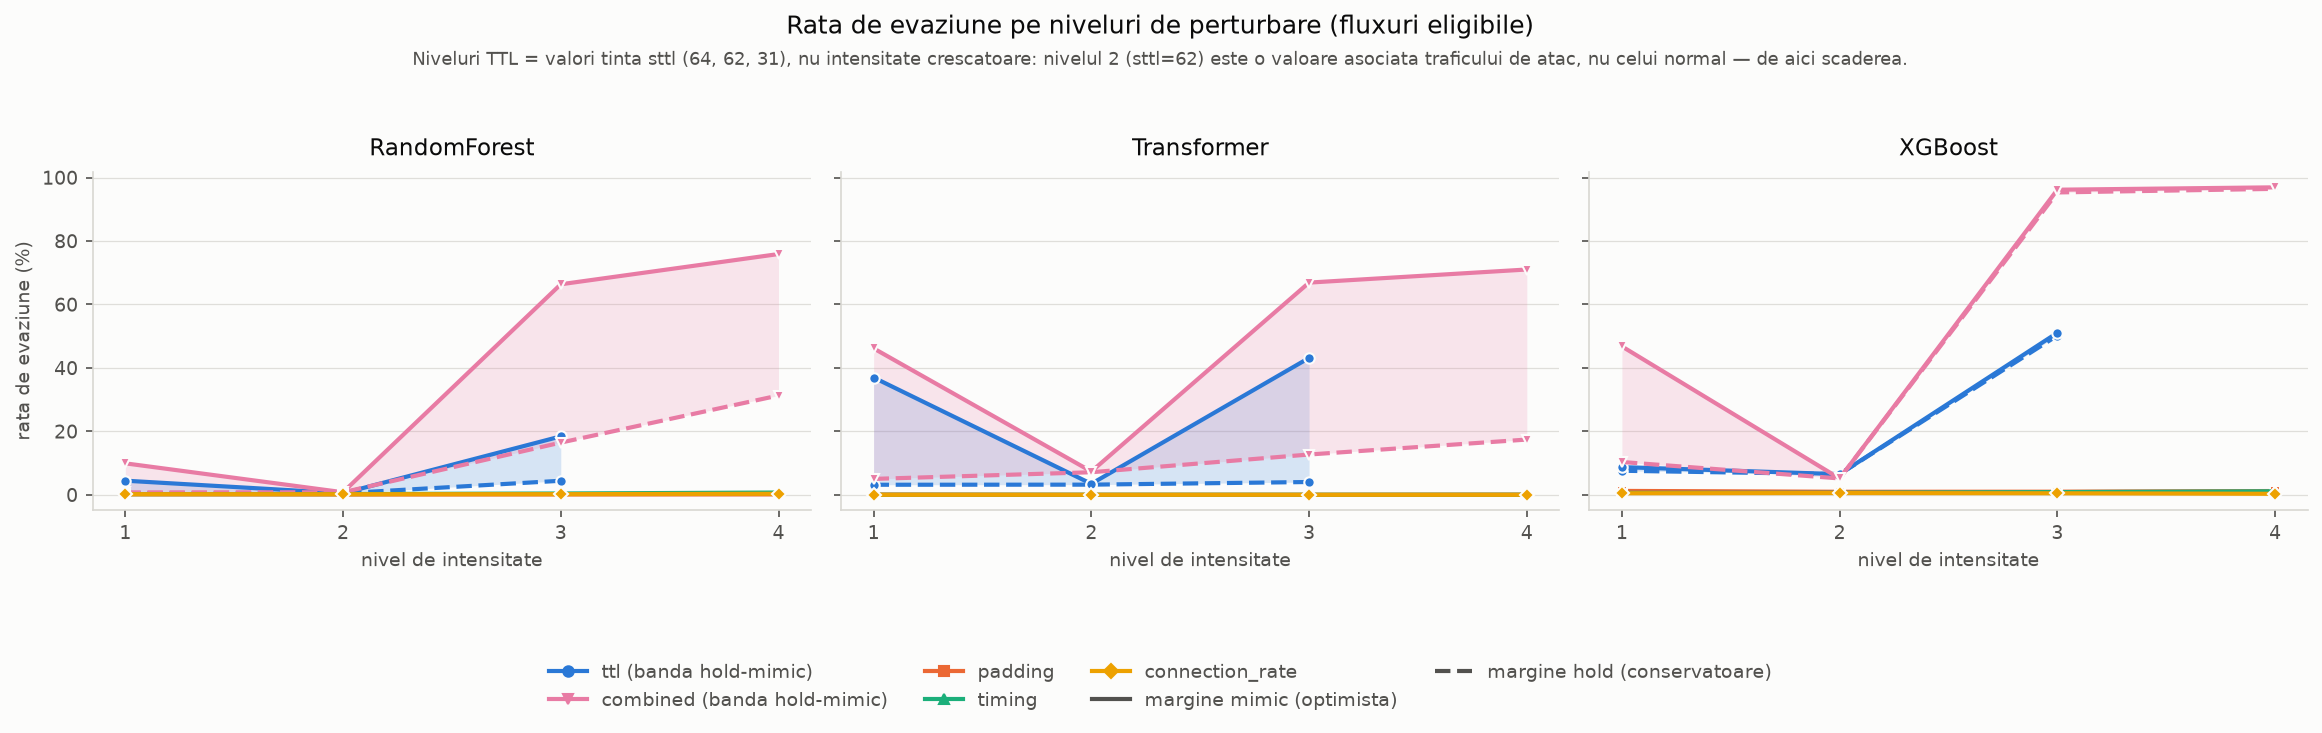
\includegraphics[width=0.95\textwidth]{figs/evasion_curves.png}
    \caption{Rata de evaziune în funcție de tipul transformării și de nivelul de intensitate}
    \label{fig:curbe}
\end{figure}

Costul practic al acestei perturbări pentru un atacator este esențial pentru interpretarea rezultatului. Modificarea valorii TTL a pachetelor emise se realizează printr-un singur apel de configurare a socketului și nu necesită nicio cunoaștere a sistemului de detecție. Valorile-țintă folosite se află peste limita inferioară discutată în subsecțiunea~\ref{subsec:admisibile}, deci rămân compatibile cu păstrarea funcționalității atacului în modelul de amenințare adoptat. Este, prin urmare, o perturbare cu cost practic nul.

\subsection{Explicația: valoarea TTL este un artefact al capturii}\label{subsec:artefact}

Analiza distribuției valorii TTL explică rezultatul. În partiția de antrenare, valoarea dominantă a traficului legitim este 31, prezentă în $70{,}5\%$ dintre fluxuri, în timp ce în fiecare clasă de atac valoarea dominantă este 254, cu ponderi care merg de la $59{,}5\%$ pe \textit{Exploits} până la $100\%$ pe \textit{Shellcode}. Această separare face ca TTL-ul sursă să fie, dintre toate cele 42 de caracteristici, cea mai corelată cu eticheta, cu un coeficient de $0{,}69$.

Separarea nu descrie însă o proprietate a atacurilor, ci una a mediului de captură: generatorul de trafic malițios s-a aflat la o distanță fixă, în număr de salturi, față de senzorul care a înregistrat traficul. Că este vorba despre o corelație și nu despre o regulă rezultă din faptul că traficul legitim conține el însuși peste 11\,000 de fluxuri cu valoarea 254, adică aproximativ o cincime din traficul legitim al partiției de antrenare.

Modelele au învățat, prin urmare, o particularitate a procesului de generare a datelor, pe care o folosesc ca principal criteriu de decizie. Perturbarea nu exploatează o slăbiciune a arhitecturii, ci una a setului de date, observație cu implicații care depășesc modelele evaluate aici.

\subsection{Nivelurile de intensitate nu formează o scară monotonă}\label{subsec:nemonoton}

Rezultatele din figura~\ref{fig:curbe} prezintă o scădere aparent anormală la nivelul intermediar al transformării TTL: pentru Transformer, rata scade de la $36{,}98\%$ la nivelul 1 la $3{,}47\%$ la nivelul 2, revenind la $43{,}15\%$ la nivelul 3.

Comportamentul nu este o eroare, ci consecința directă a modului în care sunt definite nivelurile. Ele reprezintă \emph{valori-țintă} distincte, nu intensități crescătoare ale aceleiași modificări. Valoarea corespunzătoare nivelului 2 este o valoare frecvent asociată traficului malițios în acest set, astfel încât adoptarea ei nu apropie fluxul de profilul traficului legitim.

Explicația a fost verificată prin măsurarea directă a proporției de fluxuri care ajung, sub politica optimistă, la valoarea contorului de context caracteristică traficului normal: proporția este de 100\% la nivelul 1, \textbf{0\%} la nivelul 2 și 100\% la nivelul 3. Nivelul intermediar nu produce semnătura traficului legitim, deci nu are motive să producă evaziune.

\subsection{Lățimea intervalelor}\label{subsec:latime}

Intervalele din tabelul~\ref{tab:evaziune} au lățimi foarte diferite, iar această variație este informativă. Pentru XGBoost, intervalul transformării TTL are o lățime sub o unitate procentuală ($50{,}2$ -- $51{,}1$), ceea ce arată că rezultatul nu depinde practic de ipoteza adoptată privind contorul de context. Pentru Transformer, același interval se întinde de la $4{,}0$ la $43{,}2$, deci aproape zece ori mai larg.

Interpretarea este directă: în primul caz, decizia modelului se schimbă din cauza valorii TTL însăși. În al doilea caz, o parte substanțială a efectului depinde de faptul că perturbarea reușește sau nu să reproducă și semnătura de context asociată. Raportarea unei valori unice ar fi ascuns tocmai această distincție, care este relevantă pentru evaluarea realismului atacului.

\subsection{Compoziția rezultatelor}\label{subsec:compozitie}

Tabelul~\ref{tab:compozitie} prezintă distribuția celor trei rezultate definite în subsecțiunea~\ref{subsec:rezultate} pentru transformarea TTL la intensitate maximă, sub politica optimistă.

\begin{table}[!ht]
    \caption{Compoziția rezultatelor pentru transformarea TTL la intensitate maximă (\%)}
    \centering
    \begin{tabular}{|l|c|c|c|}
        \hline
        \textbf{Model} & \textbf{Corect} & \textbf{Alt atac} & \textbf{Evaziune} \\
        \hline
        Random Forest & 65,56 & 16,02 & 18,42 \\
        \hline
        XGBoost & 40,71 & 8,22 & \textbf{51,07} \\
        \hline
        Transformer & 13,19 & \textbf{43,66} & 43,15 \\
        \hline
    \end{tabular}
    \label{tab:compozitie}
\end{table}

Cele trei modele reacționează calitativ diferit la aceeași perturbare. Random Forest păstrează clasificarea corectă pentru majoritatea fluxurilor. Modelul cu XGBoost trece direct la clasa traficului legitim. Transformer pierde aproape complet clasificarea corectă (sub 14\%) dar redistribuie fluxurile aproape în mod egal între evaziune și confuzie cu alte categorii de atac. Din perspectiva unui sistem de detecție operațional, ultimele două comportamente sunt foarte diferite: în cazul confuziei, alarma se declanșează în continuare.

Aceeași defalcare, extinsă la toate variantele și la toate cele trei modele, este prezentată în figura~\ref{fig:outcomes}. Citită pe verticală, ea arată că diferența dintre modele nu ține de o singură transformare, ci se păstrează pe întreaga grilă.

\begin{figure}[H]
    \centering
    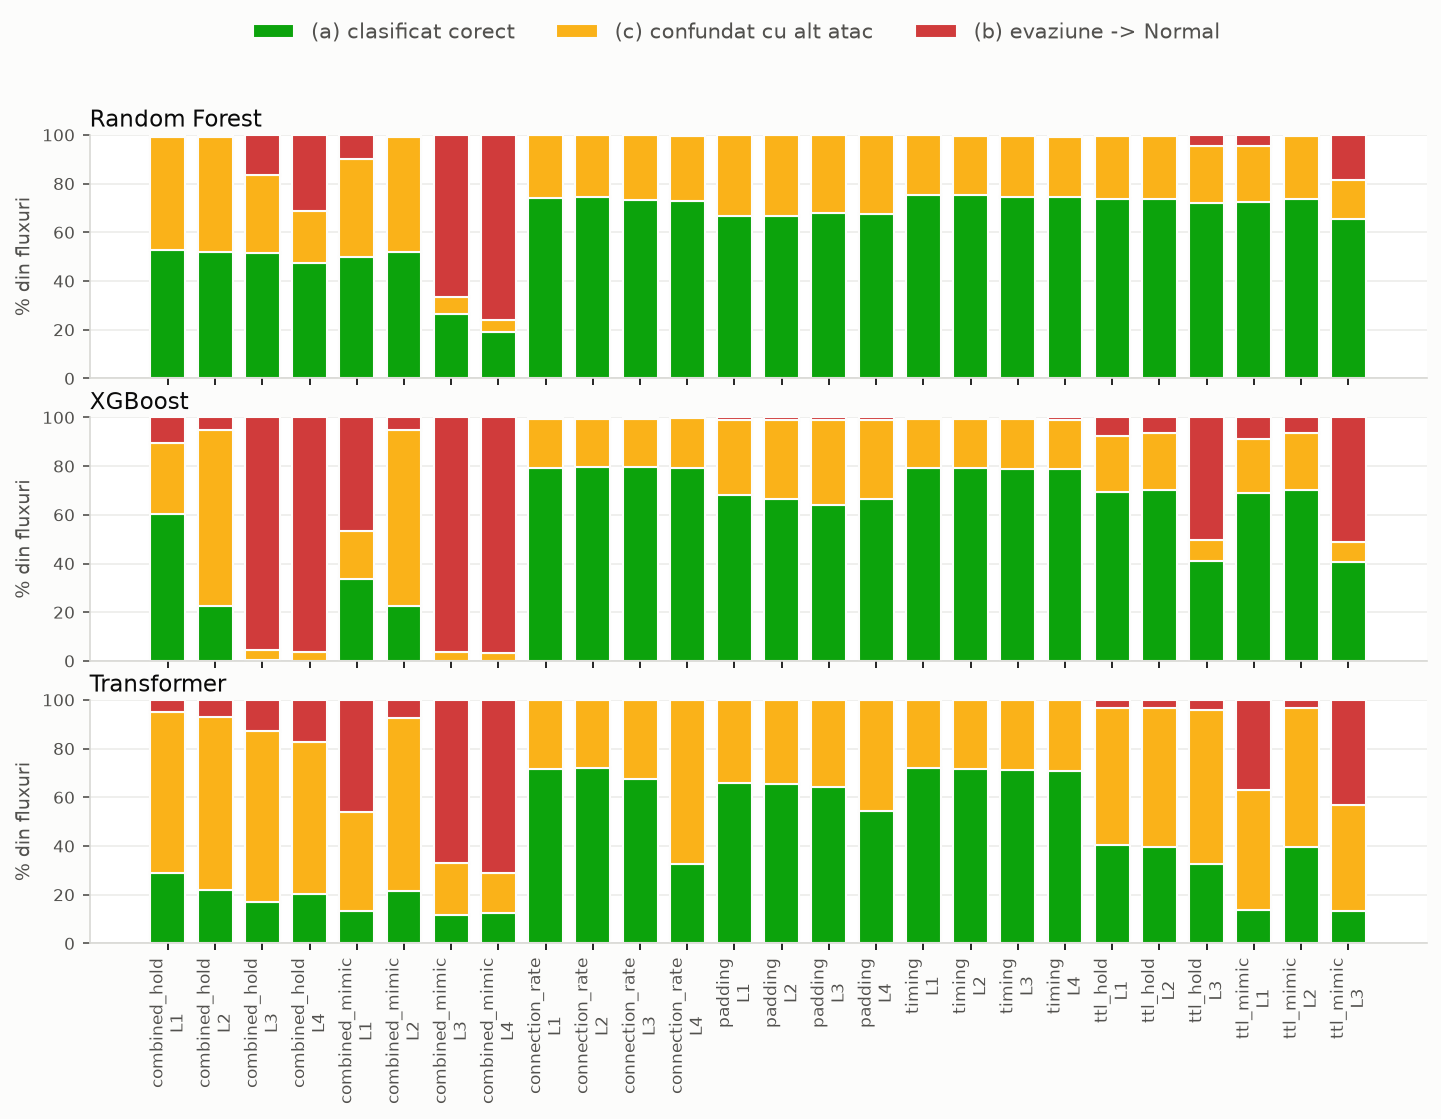
\includegraphics[width=\textwidth]{figs/evasion_outcomes_toate.png}
    \caption{Compoziția rezultatelor pe cele 26 de variante realizabile, pentru cele trei modele. Roșul apare masiv doar la variantele care ating valoarea TTL, în timp ce umplutura, temporizarea și reducerea contoarelor lasă compoziția aproape neschimbată la toate trei. Diferența dintre modele se citește pe verticală, la aceeași poziție pe axă.}
    \label{fig:outcomes}
\end{figure}

\subsection{Modificarea probabilităților de clasificare}\label{subsec:incredere}

Dincolo de eticheta finală, perturbarea modifică distribuția de probabilitate produsă de model. Tabelul~\ref{tab:incredere} prezintă valorile medii înainte și după transformarea TTL la intensitate maximă.

\begin{table}[!ht]
    \caption{Deplasarea probabilităților medii sub transformarea TTL la intensitate maximă}
    \centering
    \begin{tabular}{|l|c|c|}
        \hline
        \textbf{Model} & \textbf{$P(\textit{Normal})$} & \textbf{$P(\text{clasa reală})$} \\
        \hline
        Random Forest & 0,027 $\rightarrow$ 0,248 & 0,684 $\rightarrow$ 0,455 \\
        \hline
        XGBoost & 0,022 $\rightarrow$ 0,525 & 0,750 $\rightarrow$ 0,394 \\
        \hline
        Transformer & 0,013 $\rightarrow$ 0,419 & 0,694 $\rightarrow$ \textbf{0,148} \\
        \hline
    \end{tabular}
    \label{tab:incredere}
\end{table}

În urma perturbării, toate cele trei modele atribuie, în medie, o probabilitate mai redusă clasei reale și o probabilitate mai mare clasei normale. Cea mai mare scădere a probabilității asociate clasei reale apare în cazul Transformerului, de la 0,694 la 0,148. Pentru XGBoost, probabilitatea medie atribuită clasei normale ajunge la 0,525, depășind valoarea corespunzătoare clasei reale. Rezultatele arată că transformarea TTL afectează nu numai etichetele prezise, ci și distribuția probabilităților între clase.
\subsection{Defalcarea pe clase de atac}\label{subsec:perclasa-evaziune}

Rata globală ascunde diferențe importante între categoriile de atac. Tabelul~\ref{tab:evaziune-clase} prezintă defalcarea pentru transformarea TTL la intensitate maximă, sub politica optimistă.

\begin{table}[!ht]
    \caption{Rata de evaziune pe clase de atac, transformare TTL la intensitate maximă (\%)}
    \centering
    \begin{tabular}{|l|c|c|c|}
        \hline
        \textbf{Clasă} & \textbf{RF} & \textbf{XGB} & \textbf{Transformer} \\
        \hline
        Shellcode & 24,9 & \textbf{100,0} & 25,7 \\
        \hline
        Worms & 13,6 & \textbf{100,0} & 18,2 \\
        \hline
        Reconnaissance & 4,8 & \textbf{95,9} & 10,3 \\
        \hline
        Fuzzers & 67,7 & 89,8 & 49,8 \\
        \hline
        Exploits & 17,1 & 87,5 & 16,1 \\
        \hline
        Backdoor & 72,4 & 66,4 & 38,4 \\
        \hline
        DoS & 24,5 & 66,5 & 25,0 \\
        \hline
        Analysis & 66,1 & 63,8 & 41,4 \\
        \hline
        Generic & \textbf{1,5} & \textbf{5,5} & \textbf{67,6} \\
        \hline
    \end{tabular}
    \label{tab:evaziune-clase}
\end{table}

Se pot face trei observații.

Pentru XGBoost, toate fluxurile din clasele \textit{Shellcode} și \textit{Worms} incluse în evaluare sunt reclasificate drept trafic normal. Cele două clase sunt reprezentate prin 378, respectiv 44 de observații în partiția de testare, astfel încât valorile obținute sunt analizate în raport cu dimensiunea redusă a eșantioanelor. Această limitare este semnalată și în fișierele de rezultate. Rezultatele sugerează o vulnerabilitate mai mare a claselor slab reprezentate, însă nu sunt suficiente pentru a stabili o relație generală între frecvența unei clase și rata sa de evaziune.
A doua: clasa \textit{Generic}, cea mai bine clasificată de toate modelele conform tabelului~\ref{tab:perclasa}, rezistă aproape complet la ansamblurile de arbori, $1{,}5\%$ și $5{,}5\%$, dar cedează masiv la Transformer, cu $67{,}6\%$. Este singura clasă la care ordinea modelelor se inversează complet.

A treia: nu există o corelație simplă între calitatea clasificării inițiale și rezistența la perturbare. Clasa \textit{Analysis}, practic neclasificabilă pe trafic nemodificat, prezintă rate de evaziune comparabile cu ale unor clase bine clasificate. Rezistența la perturbare este, prin urmare, o proprietate distinctă de acuratețe, nu o consecință a ei, concluzie consistentă cu cea formulată la nivel global.

Defalcarea completă pe clase și niveluri pentru Transformer este prezentată în figura~\ref{fig:perclasa-tr}.

\begin{figure}[H]
    \centering
    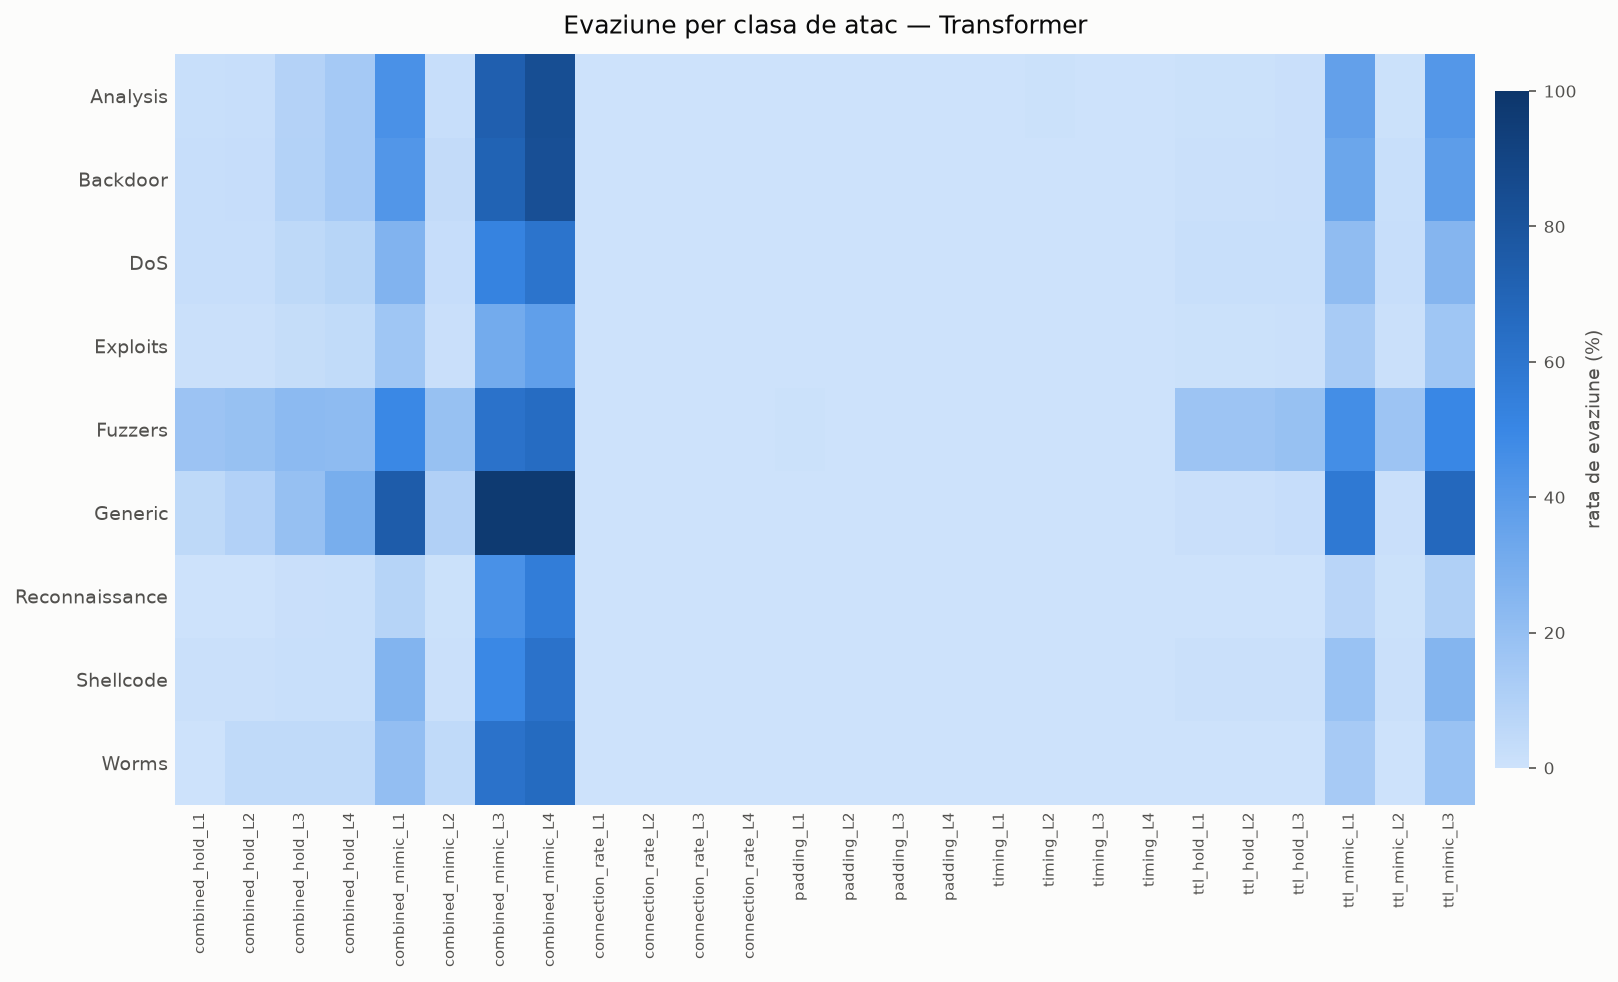
\includegraphics[width=0.92\textwidth]{figs/evasion_per_class_transformer.png}
    \caption{Rata de evaziune pe clase de atac și niveluri, pentru Transformer}
    \label{fig:perclasa-tr}
\end{figure}

\subsection{Intensitatea minimă necesară}\label{subsec:intensitate}

O rată de evaziune ridicată obținută abia la intensitatea maximă are o semnificație practică diferită de una obținută încă de la prima treaptă. Tabelul~\ref{tab:intensitate} prezintă, pentru transformarea TTL sub politica optimistă, proporția fluxurilor care evadează la un moment dat și nivelul median la care se produce prima evaziune.

\begin{table}[!ht]
    \caption{Intensitatea minimă la care se produce evaziunea (transformare TTL)}
    \centering
    \begin{tabular}{|l|c|c|r|}
        \hline
        \textbf{Model} & \textbf{Evadează} & \textbf{Nivel median} & \textbf{La nivelul 1} \\
        \hline
        Random Forest & 18,4\% & 3,0 & 2\,011 \\
        \hline
        XGBoost & 51,1\% & 3,0 & 3\,868 \\
        \hline
        Transformer & 43,2\% & \textbf{1,0} & \textbf{16\,752} \\
        \hline
    \end{tabular}
    \label{tab:intensitate}
\end{table}

Ansamblurile de arbori cedează majoritar abia la nivelul cel mai intens. Transformer are nivelul median egal cu 1: pentru aceasta, peste 16\,000 de fluxuri evadează încă de la prima treaptă de perturbare, deci nu este necesară deplasarea completă către profilul traficului legitim.

\section{Analiza de sensibilitate}\label{sec:rezultate-o4}

\subsection{Profilurile de importanță}\label{subsec:profiluri}

Tabelul~\ref{tab:importanta} prezintă primele trei caracteristici după importanța determinată prin permutare, împreună cu ponderea caracteristicii dominante în capacitatea totală de detecție.

\begin{table}[H]
    \caption{Caracteristicile cele mai importante și concentrarea capacității de detecție}
    \centering
    \begin{tabular}{|l|l|l|l|c|}
        \hline
        \textbf{Model} & \textbf{1} & \textbf{2} & \textbf{3} & \textbf{Pondere dom.} \\
        \hline
        Random Forest & TTL sursă & protocol & fereastră & 19,8\% \\
        \hline
        XGBoost & \textbf{TTL sursă} & dim. medie dest. & debit dest. & \textbf{54,6\%} \\
        \hline
        Transformer & \textbf{TTL destinație} & TTL sursă & protocol & \textbf{57,0\%} \\
        \hline
    \end{tabular}
    \label{tab:importanta}
\end{table}

Profilurile explică integral rezultatele din secțiunea~\ref{sec:rezultate-o3}. Modelul cu XGBoost concentrează $54{,}6\%$ din capacitatea sa de detecție într-o singură caracteristică, pe care atacatorul o modifică fără cost: de aici rata de evaziune de peste $50\%$. Random Forest distribuie aceeași caracteristică pe doar $19{,}8\%$, iar rata sa de evaziune este corespunzător mai mică. Comportamentul este consistent cu predicția teoretică din subsecțiunea~\ref{subsec:arbori}: selecția aleatoare a caracteristicilor la construirea nodurilor împiedică concentrarea deciziei.

Transformer prezintă profilul cel mai interesant: caracteristica sa dominantă este valoarea TTL a pachetelor \emph{de răspuns}, deci una generată de victimă și inaccesibilă atacatorului. Comparația vizuală a celor trei profiluri este prezentată în figura~\ref{fig:importanta}.

\begin{figure}[!ht]
    \centering
    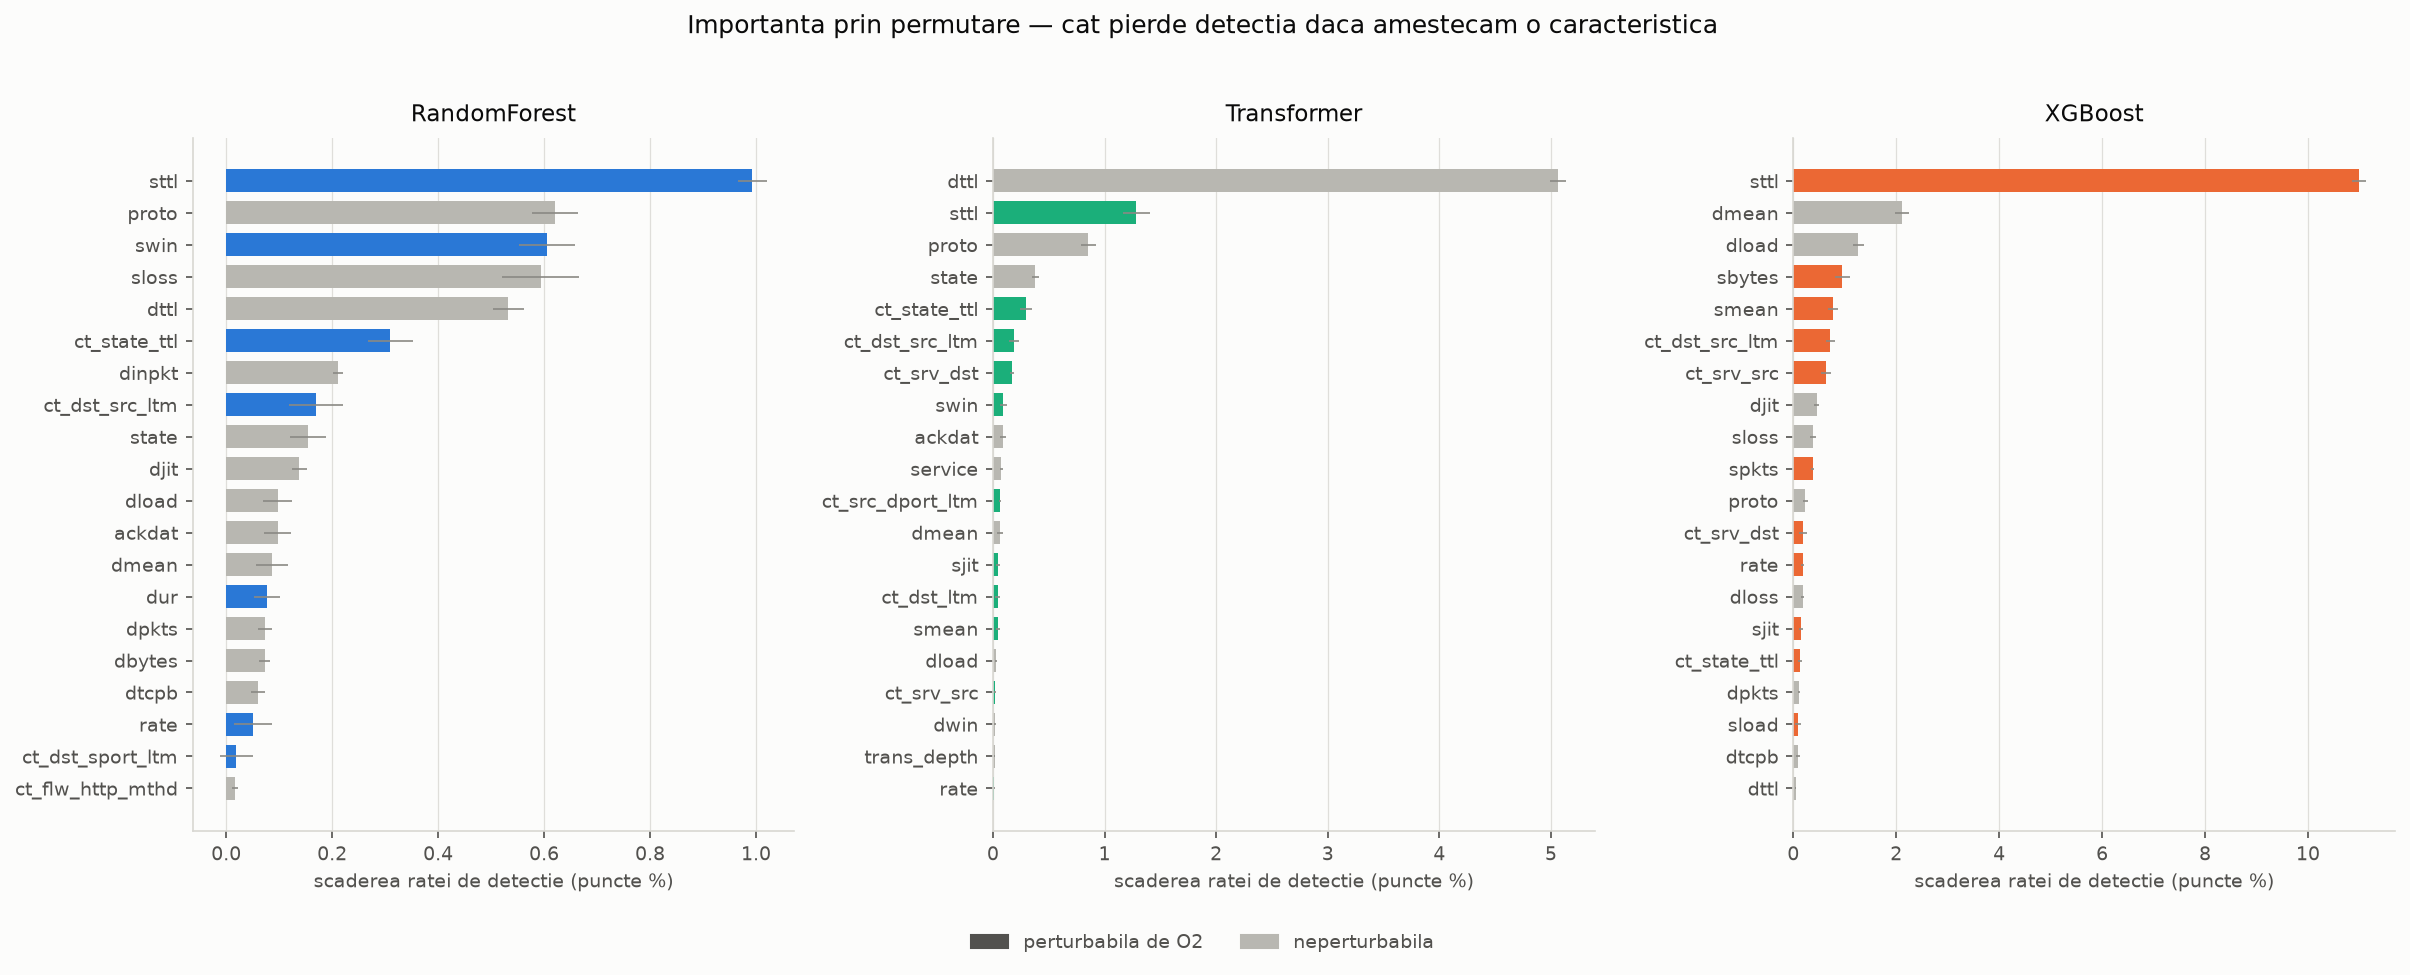
\includegraphics[width=0.95\textwidth]{figs/sensitivity_importance.png}
    \caption{Importanța prin permutare a caracteristicilor, pentru cele trei modele}
    \label{fig:importanta}
\end{figure}

\subsection{Fracțiunea accesibilă atacatorului}\label{subsec:fractiune}

Aplicând definiția fracțiunii accesibile din subsecțiunea~\ref{subsec:accesibila} se obțin valorile din tabelul~\ref{tab:accesibila}.

\begin{table}[!ht]
    \caption{Fracțiunea din capacitatea de detecție aflată la îndemâna atacatorului}
    \centering
    \begin{tabular}{|l|c|c|}
        \hline
        \textbf{Model} & \textbf{Pierdere totală} & \textbf{Fracțiune accesibilă $\rho$} \\
        \hline
        Random Forest & 5,02 & 53,6\% \\
        \hline
        XGBoost & 20,15 & \textbf{84,1\%} \\
        \hline
        Transformer & 8,89 & \textbf{26,0\%} \\
        \hline
    \end{tabular}
    \label{tab:accesibila}
\end{table}

Valorile ordonează modelele exact invers față de rezistența lor observată. Modelul cu XGBoost are $84{,}1\%$ din capacitatea de detecție în caracteristici modificabile și cedează cel mai mult. Transformer are doar $26{,}0\%$ și cedează cel mai puțin la transformările realizabile.

Aceasta este constatarea centrală a lucrării. Rezistența superioară a modelului Transformer \textbf{nu provine dintr-o reprezentare mai bună}, ci din faptul că modelul se sprijină preponderent pe informație pe care atacatorul nu o poate atinge. Distincția formulată teoretic în subsecțiunea~\ref{subsec:comparatie} este astfel tranșată empiric, în favoarea celei de-a doua explicații.

Confirmarea directă vine din varianta de referință cu constrângeri relaxate, singura care modifică și caracteristica generată de victimă. Sub această variantă, rata de evaziune a rețelei urcă la $71{,}1\%$, față de $43{,}2\%$ la transformarea realizabilă echivalentă. Prin contrast, pentru XGBoost valoarea rămâne neschimbată la $51{,}1\%$, deoarece acesta nu se sprijină semnificativ pe caracteristica respectivă. Se reamintește că această variantă nu descrie un atac practic și nu poate fi raportată alături de rezultatele realizabile, întrucât rolul ei este strict diagnostic.

\subsection{Confirmarea prin scenariul cu constrângeri relaxate}\label{subsec:relaxat}

Varianta de referință care modifică suplimentar caracteristica generată de victimă oferă o confirmare directă a interpretării. Rezultatele sunt prezentate în tabelul~\ref{tab:relaxat}.

\begin{table}[!ht]
    \caption{Comparație între transformarea realizabilă și scenariul cu constrângeri relaxate}
    \centering
    \begin{tabular}{|l|c|c|c|}
        \hline
        \textbf{Model} & \textbf{Realizabil} & \textbf{Relaxat} & \textbf{Diferență} \\
        \hline
        Random Forest & 18,4\% & 33,0\% & $+14{,}6$ \\
        \hline
        XGBoost & 51,1\% & 51,1\% & \textbf{$0{,}0$} \\
        \hline
        Transformer & 43,2\% & \textbf{71,1\%} & \textbf{$+27{,}9$} \\
        \hline
    \end{tabular}
    \label{tab:relaxat}
\end{table}

Diferențele reproduc exact ordinea prezisă de fracțiunile accesibile din tabelul~\ref{tab:accesibila}. Pentru XGBoost, relaxarea constrângerii nu schimbă absolut nimic: acesta nu folosește caracteristica generată de victimă, deci accesul suplimentar la ea nu aduce niciun avantaj atacatorului. Pentru Transformer, aceeași relaxare adaugă aproape 28 de puncte procentuale.

Valoarea scenariului relaxat este strict diagnostică: el separă întrebarea „cât de mult se sprijină modelul pe această informație” de întrebarea „cât poate obține un atacator real”.

\subsection{Corelația dintre importanță și evaziune}\label{subsec:corelatie}

Obiectivul formulat în capitolul~\ref{ch:obiective} cere punerea în corespondență a ratei de evaziune cu importanța caracteristicilor afectate. Tabelul~\ref{tab:corelatie} prezintă coeficienții de corelație a rangurilor, calculați pe cele 26 de variante realizabile.

\begin{table}[!ht]
    \caption{Corelația dintre masa de importanță afectată și rata de evaziune}
    \centering
    \begin{tabular}{|l|c|c|c|}
        \hline
        \textbf{Model} & \textbf{$\rho$ Spearman} & \textbf{$p$} & \textbf{$n$} \\
        \hline
        Random Forest & \textbf{0,954} & $<0{,}0001$ & 26 \\
        \hline
        XGBoost & 0,882 & $<0{,}0001$ & 26 \\
        \hline
        Transformer & 0,830 & $<0{,}0001$ & 26 \\
        \hline
    \end{tabular}
    \label{tab:corelatie}
\end{table}

Corelațiile sunt puternice și semnificative pentru toate cele trei modele: transformările care afectează o masă mai mare de importanță produc o evaziune mai mare. Relația este ilustrată în figura~\ref{fig:corelatie}.

\begin{figure}[!ht]
    \centering
    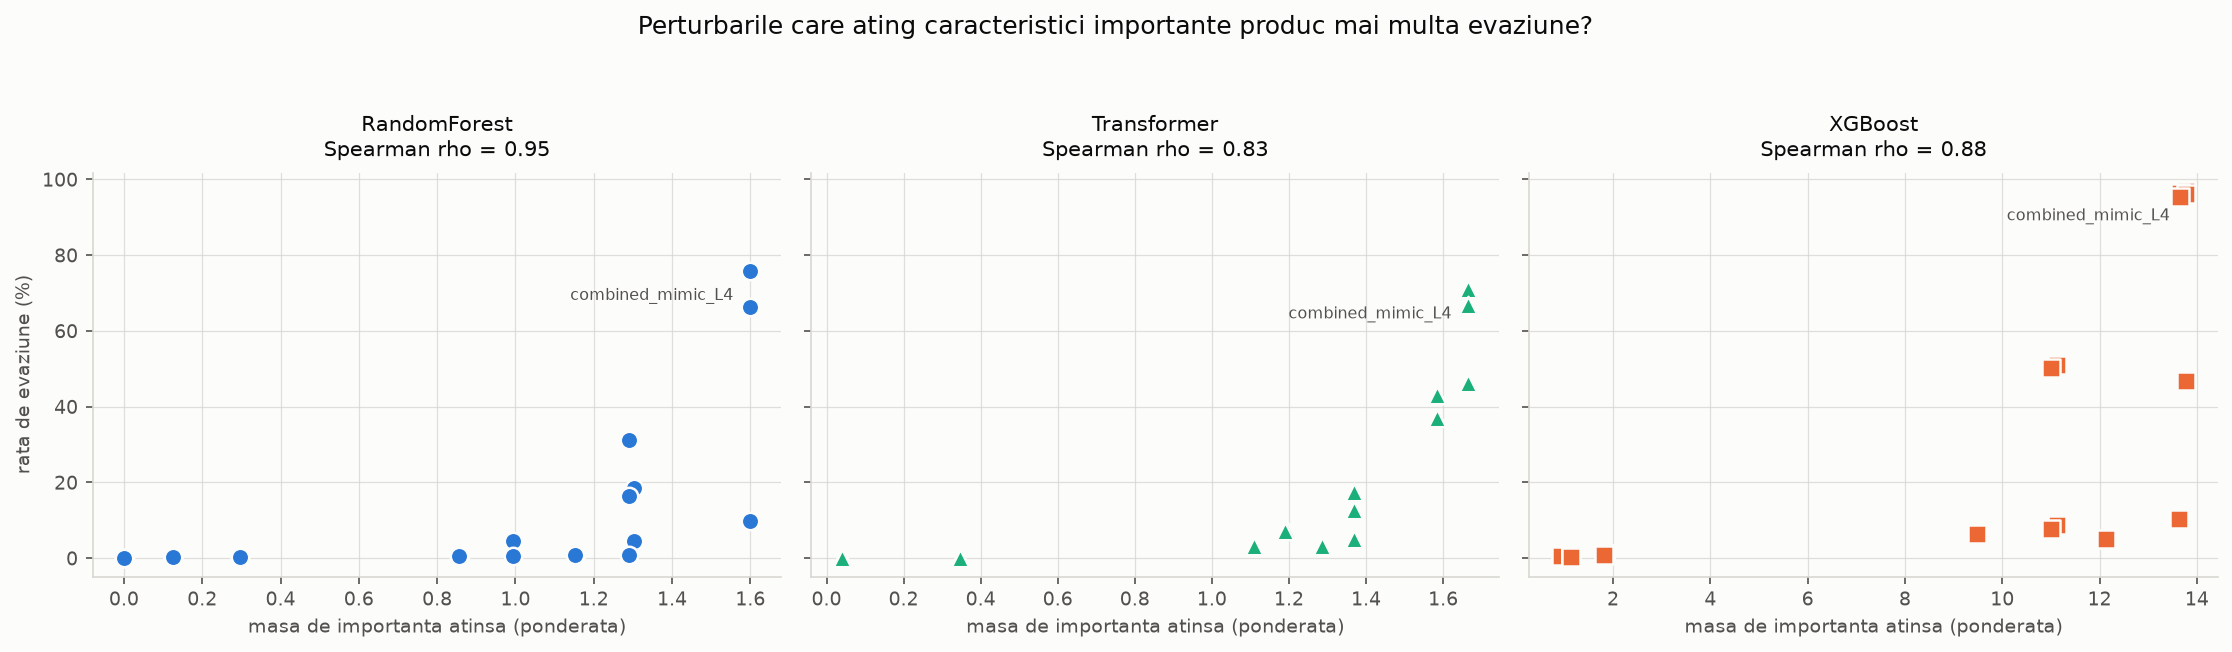
\includegraphics[width=0.88\textwidth]{figs/sensitivity_importance_vs_evasion.png}
    \caption{Relația dintre masa de importanță afectată și rata de evaziune}
    \label{fig:corelatie}
\end{figure}

Rezultatul validează metodologia: importanța determinată prin permutare, calculată independent de experimentul de evaziune, prezice ce transformări vor fi eficiente. Alegerea metricii comensurabile din subsecțiunea~\ref{subsec:comensurabil} este cea care face posibilă această comparație directă.

\subsection{Clasele atractor}\label{subsec:atractor}

Analiza rezultatului de tip (c) arată că fluxurile care rămân semnalate nu se distribuie uniform între clasele de atac, ci converg către o clasă preferată, diferită pentru fiecare model. Pentru XGBoost, între $67{,}6\%$ și $95{,}8\%$ dintre fluxurile provenite din orice clasă sursă ajung la clasa \textit{Analysis}. Pentru Random Forest, clasa preferată este \textit{Backdoor}, iar pentru Transformer, \textit{DoS}.

Fenomenul nu este întâmplător. Clasele \textit{Analysis} și \textit{Backdoor} sunt exact cele cu cele mai slabe scoruri $F1$ din tabelul~\ref{tab:perclasa}, cu valori între $0{,}003$ și $0{,}116$. Clasa atractor este regiunea din spațiul caracteristicilor în care modelul nu are un angajament ferm: atunci când perturbarea îndepărtează fluxul de clasa sa, acesta este împins către zona de incertitudine maximă. Distribuția destinațiilor este prezentată în figura~\ref{fig:destinatii}.

\begin{figure}[H]
    \centering
    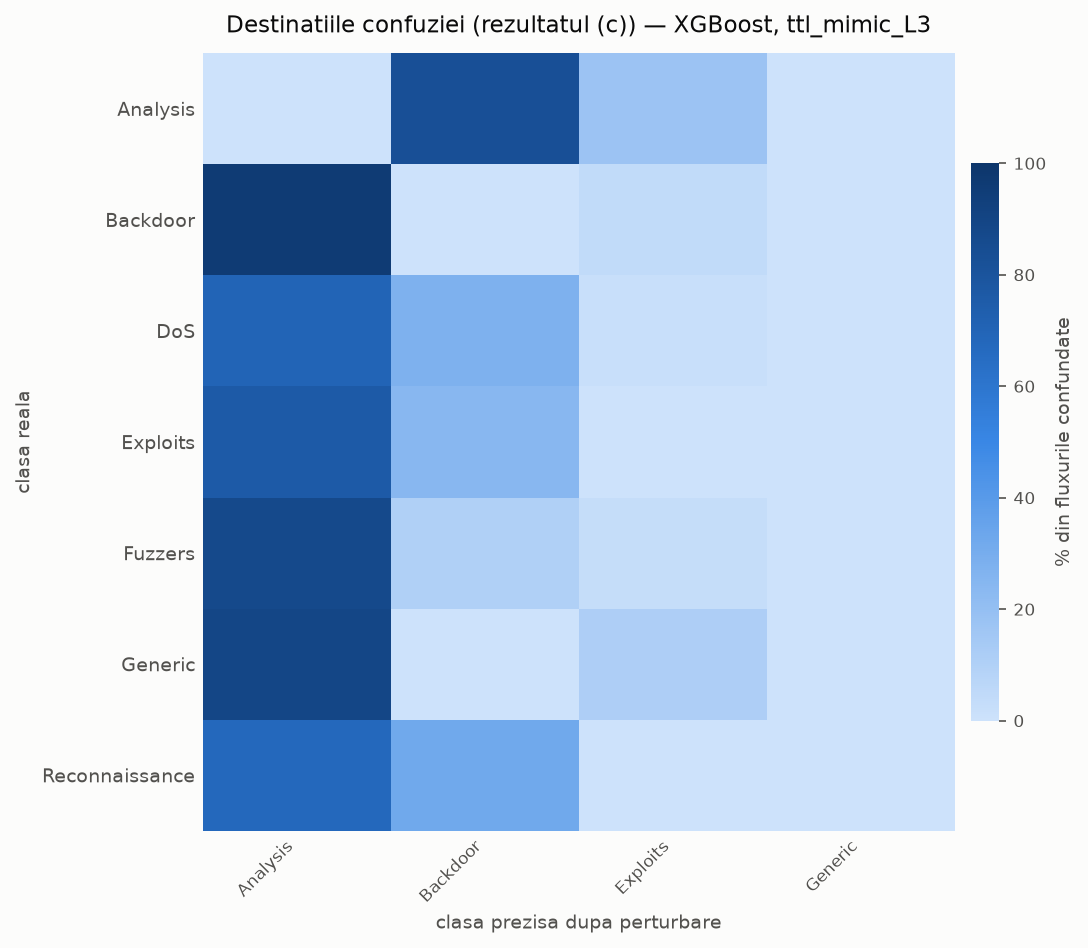
\includegraphics[width=0.88\textwidth]{figs/sensitivity_destinations_xgboost.png}
    \caption{Distribuția claselor de destinație pentru fluxurile perturbate care rămân semnalate}
    \label{fig:destinatii}
\end{figure}

\subsection{Proximitatea față de granița de decizie}\label{subsec:proximitate}

Se pune întrebarea dacă fluxurile care evadează erau deja incerte înainte de perturbare. Tabelul~\ref{tab:proximitate} compară probabilitatea medie atribuită clasei reale, pe traficul nemodificat, pentru fluxurile care ulterior evadează față de cele care nu evadează.

\begin{table}[!ht]
    \caption{Încrederea inițială a modelului, pentru fluxurile care evadează și pentru celelalte}
    \centering
    \begin{tabular}{|l|c|c|c|}
        \hline
        \textbf{Model} & \textbf{Evadate} & \textbf{Ne-evadate} & \textbf{Diferență} \\
        \hline
        Random Forest & 0,359 & 0,757 & \textbf{$+0{,}398$} \\
        \hline
        XGBoost & 0,653 & 0,850 & $+0{,}197$ \\
        \hline
        Transformer & 0,806 & 0,609 & \textbf{$-0{,}197$} \\
        \hline
    \end{tabular}
    \label{tab:proximitate}
\end{table}

Pentru ansamblurile de arbori, diferența este pozitivă și substanțială: evaziunea se concentrează pe fluxurile față de care modelul era deja nesigur, ceea ce corespunde intuiției. Pentru Transformer, diferența este \textbf{negativă}: modelul cedează tocmai pe fluxurile de care era \emph{mai} sigur.

Rezultatul este contraintuitiv și are o implicație practică importantă: încrederea ridicată a acestui model nu constituie un indicator de robustețe. Un mecanism de apărare care ar trata predicțiile de încredere mare drept fiabile ar fi ineficient exact acolo unde este mai necesar.

\subsection{Limita atribuirii pe o singură caracteristică}\label{subsec:limitaatrib}

Analiza res\-trân\-să la clasa \textit{Generic} ilus\-trea\-ză li\-mi\-ta\-rea an\-ti\-ci\-pa\-tă te\-o\-re\-tic în subsecțiunea~\ref{subsec:limita}. Pentru Transformer, importanța se distribuie pe această clasă între trei caracteristici cu ponderi apropiate, $33{,}8\%$, $32{,}9\%$ și $23{,}1\%$, niciuna dintre ele nefiind, luată separat, suficientă pentru a explica prăbușirea detecției observată sub perturbare.

Constatarea confirmă că importanța atribuită individual constituie o limită inferioară a vulnerabilității, nu o estimare a ei, și justifică retroactiv decizia centrală de proiectare din capitolul~\ref{ch:analysis}: propagarea consistentă a dependențelor. O metodologie care ar fi perturbat caracteristicile izolat, fără propagare, nu ar fi produs substituția coerentă necesară și ar fi subestimat sistematic vulnerabilitatea măsurată.

Această etapă a necesitat și o corecție de implementare, descrisă în secțiunea~\ref{sec:implsensibilitate}: pe o singură clasă, permutarea internă a valorilor nu rupe legătura cu eticheta atunci când caracteristica este cvasiconstantă în interiorul clasei, iar importanța apare fals ca nulă. Substituția dintr-o distribuție donoare externă a corectat măsurătoarea.

\section{Efectul antrenării adversariale}\label{sec:rezultate-o6}

Secțiunea prezintă rezultatele obținute prin reantrenarea celor trei clasificatoare pe seturi care conțin variante perturbate, conform construcției din secțiunea~\ref{sec:antrenare}. Verificările de integritate ale montajului au fost prezentate separat în subsecțiunea~\ref{subsec:val-adversarial} și au precedat citirea oricărui rezultat.

\subsection{Configurația experimentului}\label{subsec:o6-config}

Au fost antrenate treizeci de modele: trei grupuri, trei repetări cu \textit{seed}-uri distincte și trei familii de clasificatoare, la care se adaugă un al patrulea grup, cu o singură repetare, destinat testului de generalizare din subsecțiunea~\ref{subsec:o6-generalizare}. Compoziția seturilor este cea din subsecțiunea~\ref{subsec:val-adversarial}: 294\,682 de rânduri pentru ambele grupuri augmentate, identice ca dimensiune și distribuție a claselor.

Antrenarea a durat 89 de minute pentru ansamblurile de arbori și 282 de minute pentru Transformer, cele două putând rula simultan întrucât folosesc resurse diferite. Evaluarea celor treizeci de modele a durat 26 de minute.

Un rezultat colateral al antrenării merită consemnat, pentru că privește stabilitatea măsurătorilor care urmează. Numărul de epoci până la cel mai bun scor de validare a variat, la cele zece rulări ale rețelei, între 10 și 48, deși în interiorul unui grup singura diferență între rulări este \textit{seed}-ul. Amplitudinea confirmă necesitatea repetării: un grup de control evaluat cu un singur \textit{seed} ar fi putut proveni din oricare dintre cele două extreme.

\subsection{Mulțimea comună de măsurare}\label{subsec:o6-cohorta}

Ratele de evaziune se raportează la intersecția fluxurilor semnalate pe trafic nemodificat de toate rulările aceleiași familii, conform subsecțiunii~\ref{subsec:cohorta}. Dimensiunile obținute sunt prezentate în tabelul~\ref{tab:o6-cohorte}.

\begin{table}[!ht]
    \caption{Mulțimea comună per familie de modele}
    \centering
    \begin{tabular}{|l|c|c|c|}
        \hline
        \textbf{Model} & \textbf{Eligibile per rulare} & \textbf{Mulțimea comună} & \textbf{Din fluxurile de atac} \\
        \hline
        Random Forest & 45\,106--45\,250 & 45\,001 & 99,27\,\% \\
        \hline
        XGBoost & 44\,237--44\,658 & 43\,637 & 96,26\,\% \\
        \hline
        Transformer & 45\,173--45\,307 & 44\,982 & 99,23\,\% \\
        \hline
    \end{tabular}
    \label{tab:o6-cohorte}
\end{table}

Intersecția a costat între 0,7\,\% și 3,7\,\% din fluxurile de atac, deci comparațiile se fac practic pe întreaga populație, nu pe un rest îngust. Această mulțime a fost construită împotriva unei situații anume, aceea în care un model pare robust doar pentru că semnalează mai puține fluxuri și are astfel un numitor mai mic. Situația nu s-a produs.

\subsection{Performanța pe trafic nemodificat}\label{subsec:o6-curat}

Tabelul~\ref{tab:o6-curat} prezintă metricile pe partiția de testare, mediate peste repetări.

\begin{table}[!ht]
    \caption{Performanța pe traficul nemodificat, medie peste trei repetări}
    \centering
    \begin{tabular}{|l|ccc|ccc|}
        \hline
        \textbf{Model} & \multicolumn{3}{c|}{\textbf{Macro-$F1$}}
                       & \multicolumn{3}{c|}{\textbf{$F1$ ponderat}} \\
        \cline{2-7}
                       & O1 & C1 & O6 & O1 & C1 & O6 \\
        \hline
        Random Forest       & 0,5010 & 0,4973 & 0,4818 & 0,7421 & 0,7366 & 0,7344 \\
        \hline
        XGBoost & 0,5089 & 0,5150 & 0,4948 & 0,7813 & 0,7624 & 0,7714 \\
        \hline
        Transformer       & 0,4468 & 0,4432 & 0,4246 & 0,7236 & 0,7234 & 0,7170 \\
        \hline
    \end{tabular}
    \label{tab:o6-curat}
\end{table}

Costul augmentării pe traficul nemodificat este mic: macro-$F1$ scade cu 0,0192 la Random Forest, 0,0141 la XGBoost și 0,0222 la rețea, față de grupul de referință. Acuratețea echilibrată urmează același tipar, cu o excepție notabilă: la rețea ea rămâne practic neschimbată, 0,6174 față de 0,6140, ceea ce arată că pierderea de macro-$F1$ provine din precizie, nu din sensibilitate. Pentru rețea, abaterea standard între repetări este 0,0127, adică de același ordin cu efectul măsurat, ceea ce limitează precizia cu care acest cost poate fi enunțat.

\subsection{Rata de evaziune}\label{subsec:o6-evaziune}

Rezultatul principal este prezentat în tabelul~\ref{tab:o6-evaziune}. Valoarea raportată este maximul peste cele 26 de variante realizabile, conform argumentului din subsecțiunea~\ref{subsec:cohorta}: atacatorul alege transformarea care îi convine, nu una la întâmplare.

\begin{table}[!ht]
    \caption{Evaziunea în cel mai rău caz realizabil, pe mulțimea comună, medie $\pm$ abatere standard peste trei repetări}
    \centering
    \begin{tabular}{|l|c|c|c|}
        \hline
        \textbf{Model} & \textbf{O1} & \textbf{C1} & \textbf{O6} \\
        \hline
        Random Forest       & 80,32 $\pm$ 4,32\,\% & 75,51 $\pm$ 0,41\,\% & \textbf{0,18 $\pm$ 0,04\,\%} \\
        \hline
        XGBoost & 96,90 $\pm$ 0,05\,\% & 96,24 $\pm$ 0,20\,\% & \textbf{0,46 $\pm$ 0,07\,\%} \\
        \hline
        Transformer       & 70,92 $\pm$ 8,55\,\% & 72,52 $\pm$ 5,81\,\% & \textbf{0,19 $\pm$ 0,07\,\%} \\
        \hline
    \end{tabular}
    \label{tab:o6-evaziune}
\end{table}

Reducerea este cu un ordin de mărime peste pragul stabilit înaintea rulării. Ea nu se limitează la varianta cea mai agresivă: mediana peste variantele realizabile scade de la 0,44\,\% la 0,01\,\% pentru Random Forest, de la 4,45\,\% la 0,01\,\% pentru XGBoost și de la 3,00\,\% la 0,02\,\% pentru Transformer. Curbele complete sunt prezentate în figura~\ref{fig:o6-curbe}.

\begin{figure}[H]
    \centering
    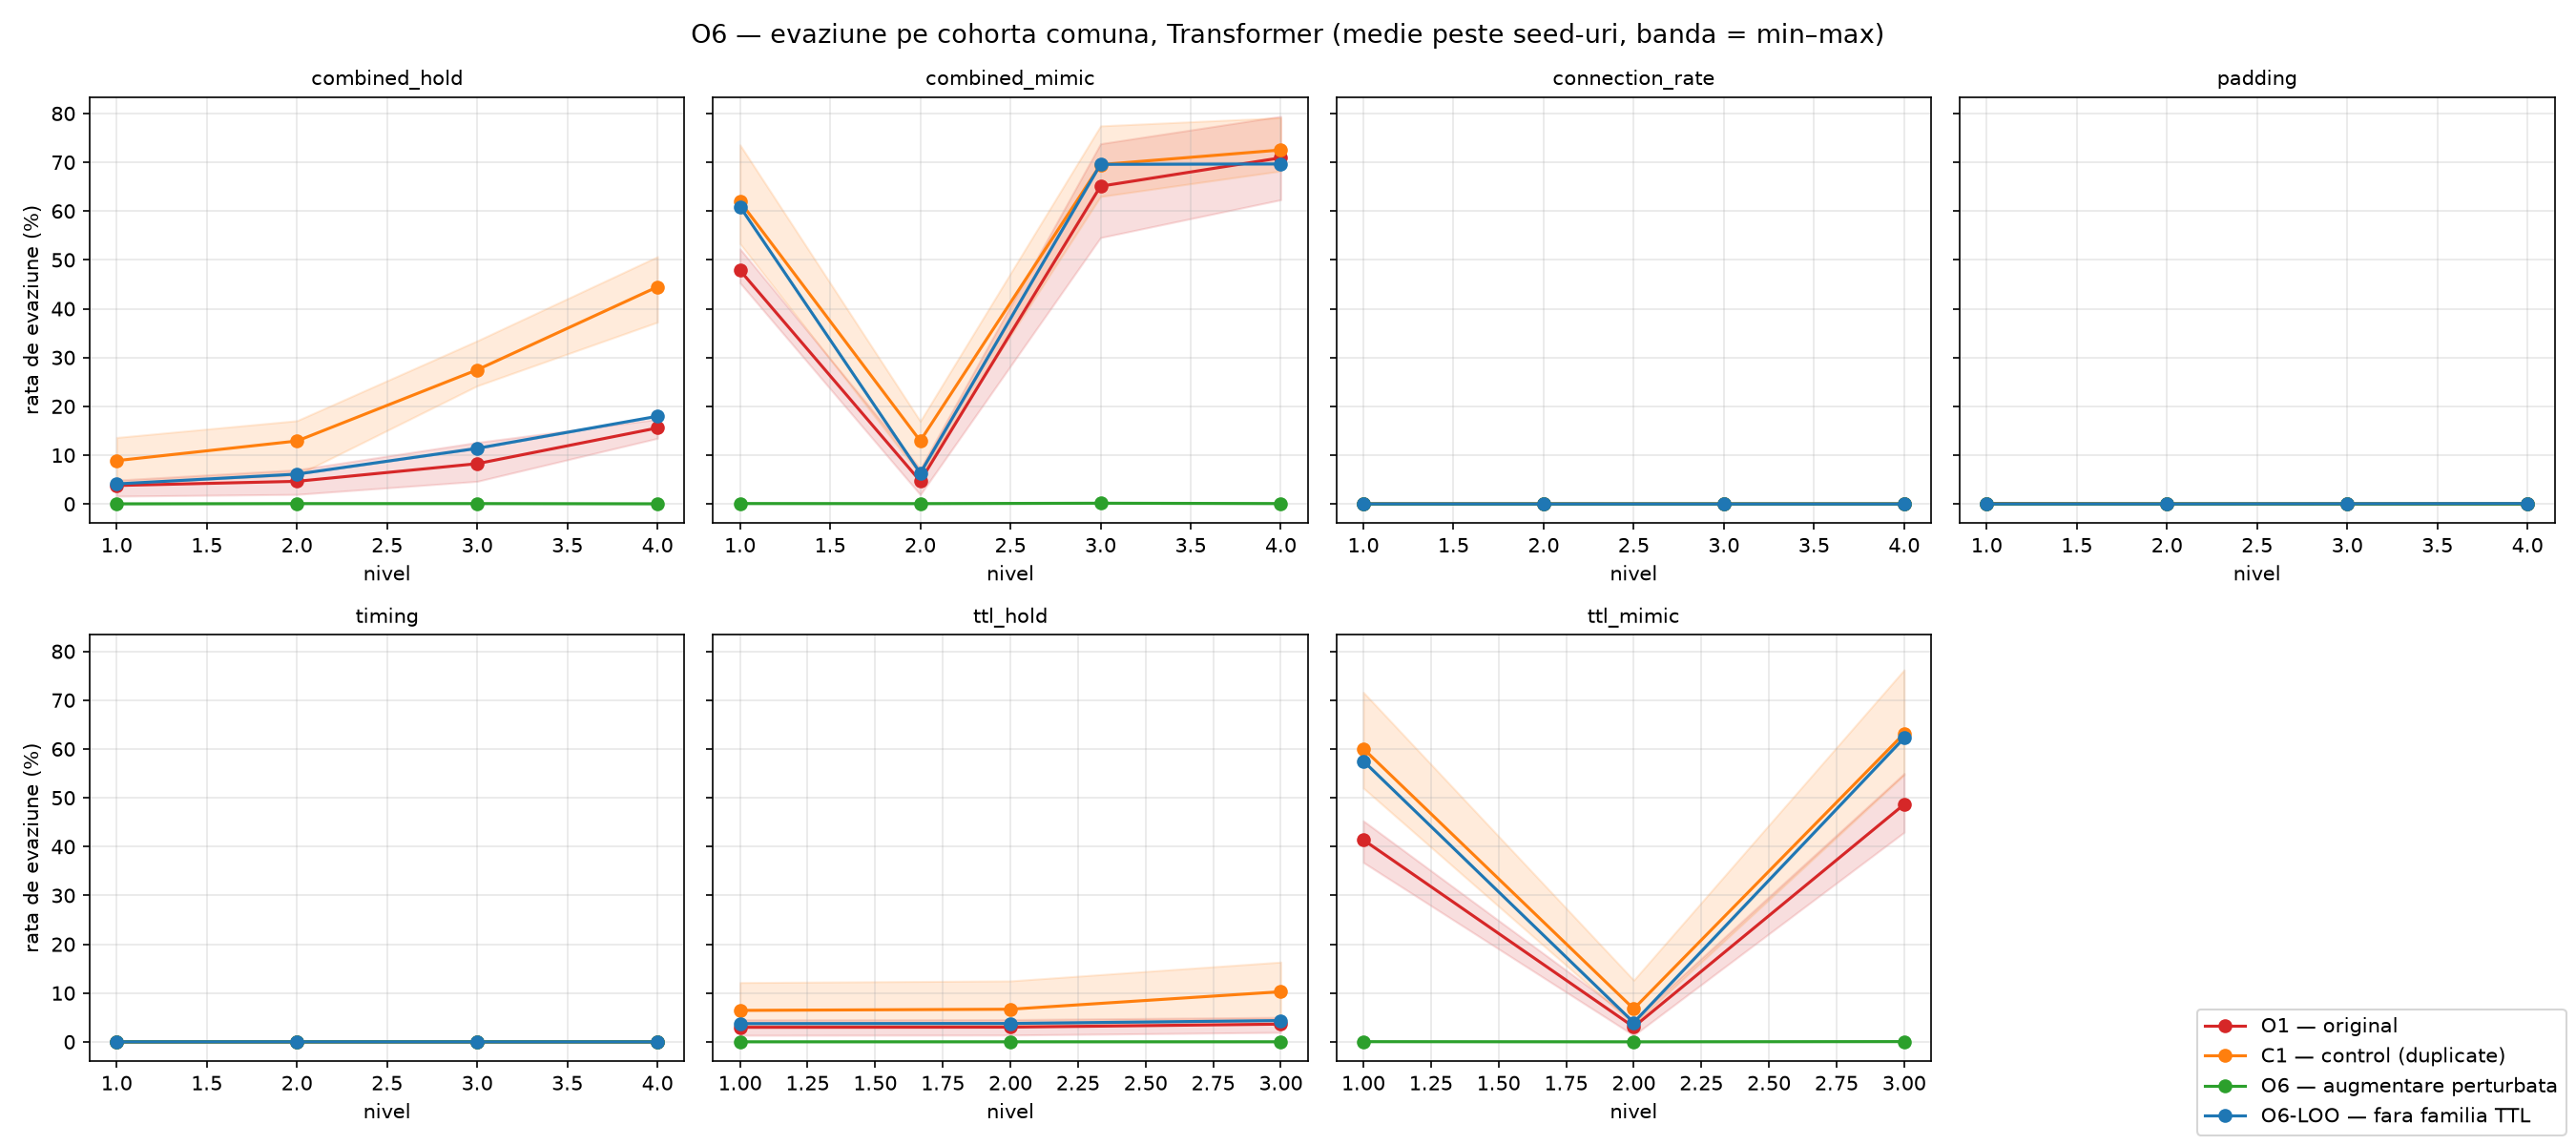
\includegraphics[width=\textwidth]{figs/o6_evasion_curves_transformer.png}
    \caption{Rata de evaziune pe mulțimea comună, per familie de transformări și nivel, pentru Transformer. Banda indică intervalul dintre repetări. Grupul antrenat fără familia TTL urmărește îndeaproape grupul de control tocmai pe transformările pe care nu le-a văzut.}
    \label{fig:o6-curbe}
\end{figure}

Două observații privind grupul de control. Prima: pentru Transformer, adăugarea de copii \emph{neperturbate} a înrăutățit situația, evaziunea crescând de la 70,92\,\% la 72,52\,\%, iar pe varianta \verb|ttl_mimic_L1| de la 41,39\,\% la 60,07\,\%. Dacă rezultatul ar fi fost raportat prin comparație directă cu grupul de referință, o parte din câștigul atribuit perturbării ar fi fost, de fapt, repararea unei degradări produse de volumul suplimentar de date. A doua: abaterea standard între repetări este de 8,55 puncte procentuale pentru grupul de referință al modelului Transformer și sub 0,08 pentru toate grupurile apărate. Antrenarea adversarială nu doar coboară rata, ci elimină și variabilitatea ei între repetări.

\subsection{Natura rezultatului: invarianță, nu alarmă permanentă}\label{subsec:o6-compozitie}

O reducere de la 96,90\,\% la 0,00\,\% ridică în mod firesc suspiciunea că modelul a învățat să declare atac pentru orice intrare, ceea ce ar elimina evaziunea distrugând utilitatea sistemului. Defalcarea celor trei rezultate posibile, prezentată în tabelul~\ref{tab:o6-compozitie}, arată că nu aceasta este explicația.

\begin{table}[!ht]
    \caption{Compoziția rezultatelor la varianta cea mai agresivă (\texttt{combined\_mimic}, nivel 4), pe mulțimea comună}
    \centering
    \begin{tabular}{|l|l|c|c|c|}
        \hline
        \textbf{Model} & \textbf{Grup} & \textbf{Corect} & \textbf{Alt tip de atac} & \textbf{Evadat} \\
        \hline
        Random Forest       & O1 & 14,80\,\% & 4,88\,\%  & 80,32\,\% \\
        \hline
        Random Forest       & O6 & \textbf{75,82\,\%} & 24,00\,\% & \textbf{0,18\,\%} \\
        \hline
        XGBoost & O1 & 0,13\,\%  & 2,97\,\%  & 96,90\,\% \\
        \hline
        XGBoost & O6 & \textbf{77,15\,\%} & 22,85\,\% & \textbf{0,00\,\%} \\
        \hline
        Transformer       & O1 & 12,88\,\% & 16,21\,\% & 70,92\,\% \\
        \hline
        Transformer       & O6 & \textbf{67,87\,\%} & 32,04\,\% & \textbf{0,09\,\%} \\
        \hline
    \end{tabular}
    \label{tab:o6-compozitie}
\end{table}

Comparația care contează este cu proporția clasificărilor corecte pe traficul \emph{nemodificat}, măsurată pe aceeași mulțime: 75,15\,\% pentru Random Forest, 78,97\,\% pentru XGBoost și 72,69\,\% pentru rețea. Modelele apărate clasifică fluxurile puternic perturbate aproape la fel de exact ca pe cele neatinse. Transformarea a devenit, pentru ele, aproape invizibilă.

Confirmarea independentă vine de la clasa traficului legitim, unde o strategie de tip alarmă permanentă ar produce o prăbușire imediată: scorul $F1$ pe această clasă scade de la 0,7665 la 0,7522 pentru Random Forest, de la 0,8467 la 0,8308 pentru XGBoost și de la 0,7380 la 0,7348 pentru rețea.

\subsection{Costul per clasă}\label{subsec:o6-perclasa}

Metricile globale ascund însă o degradare importantă, pe care criteriul de siguranță formulat în subsecțiunea~\ref{subsec:preinregistrare} a fost construit tocmai pentru a o detecta. Tabelul~\ref{tab:o6-worms} prezintă evoluția clasei \textit{Worms}, cea mai rară din set, cu 130 de exemple la antrenare și 44 la testare.

\begin{table}[!ht]
    \caption{Scorul $F1$ pe clasa \textit{Worms}, medie peste repetări}
    \centering
    \begin{tabular}{|l|c|c|c|c|c|}
        \hline
        \textbf{Model} & \textbf{O1} & \textbf{C1} & \textbf{O6} & \textbf{O6\,--\,O1} & \textbf{O6\,--\,C1} \\
        \hline
        Random Forest       & 0,5871 & 0,5014 & 0,4604 & $-0{,}127$ & $-0{,}041$ \\
        \hline
        XGBoost & 0,4907 & 0,5974 & 0,4159 & $-0{,}075$ & $\mathbf{-0{,}182}$ \\
        \hline
        Transformer       & 0,2216 & 0,1977 & 0,0942 & $-0{,}127$ & $-0{,}104$ \\
        \hline
    \end{tabular}
    \label{tab:o6-worms}
\end{table}

Descompunerea pe cele două grupuri arată că sursa degradării diferă de la un model la altul. La Random Forest, două treimi din pierdere sunt prezente deja în grupul de control, deci provin din deplasarea proporției dintre clase, nu din perturbare. La XGBoost situația este inversă: grupul de control a \emph{îmbunătățit} clasa, iar perturbarea a costat ulterior 0,182, cea mai mare pierdere înregistrată.

Nicio altă clasă nu depășește pragul de 0,05 la niciun model. Rezultatul confirmă valoarea raportării per clasă: pierderea globală de macro-$F1$ a rețelei este de 0,022, în timp ce clasa \textit{Worms} pierde mai mult de jumătate din scorul ei.

\subsection{Generalizarea la o familie de transformări nevăzută}\label{subsec:o6-generalizare}

Rezultatele de până acum măsoară robustețea la exact familia de transformări folosită la antrenare. Ele nu pot distinge între două situații foarte diferite: un model care a învățat proprietatea care face transformările eficiente și unul care a memorat transformările înseși. Distincția se poate face doar excluzând o familie din antrenare și măsurând tocmai pe ea, procedeu anunțat printre ipotezele din secțiunea~\ref{sec:ipoteze}.

Grupul O6-LOO a fost antrenat fără nicio variantă din familia TTL, rămânând doar cu umplutura, temporizarea și reducerea contoarelor de conexiuni, apoi a fost măsurat pe familia exclusă. Rezultatele sunt prezentate în tabelul~\ref{tab:o6-loo}.

\begin{table}[!ht]
    \caption{Evaziunea pe familia TTL, exclusă complet din antrenarea grupului O6-LOO}
    \centering
    \begin{tabular}{|l|c|c|c|c|}
        \hline
        \textbf{Model} & \textbf{O1} & \textbf{C1} & \textbf{O6-LOO} & \textbf{O6} \\
        \hline
        Random Forest       & 80,32\,\% & 75,51\,\% & \textbf{11,84\,\%} & 0,18\,\% \\
        \hline
        XGBoost & 96,90\,\% & 96,24\,\% & \textbf{95,68\,\%} & 0,46\,\% \\
        \hline
        Transformer       & 70,92\,\% & 72,52\,\% & \textbf{69,65\,\%} & 0,19\,\% \\
        \hline
    \end{tabular}
    \label{tab:o6-loo}
\end{table}

Rezultatul separă net cele trei modele. Random Forest generalizează: fără să fi văzut vreodată o modificare de TTL, ea coboară de la 80,32\,\% la 11,84\,\% pe varianta combinată de nivel maxim și de la 19,60\,\% la 10,88\,\% pe \verb|ttl_mimic| de nivel 3. Invarianța învățată pe umplutură și temporizare s-a transferat unei familii pe care nu a întâlnit-o.

Celelalte două modele nu generalizează deloc. Transformer rămâne la 69,65\,\% față de 70,92\,\% în grupul de referință, iar pe varianta \verb|combined_mimic| de nivel 1 se înrăutățește, de la 47,86\,\% la 60,91\,\%. Modelul cu XGBoost coboară nesemnificativ în ansamblu, de la 96,90\,\% la 95,68\,\%, dar pe două variante devine substanțial mai vulnerabil: pe \verb|ttl_hold| de nivel 3 evaziunea crește de la 49,16\,\% la 90,72\,\%, iar pe \verb|ttl_mimic| de nivel 3 de la 49,89\,\% la 92,44\,\%. Antrenarea pe transformări care nu produceau evaziune l-a făcut mai vulnerabil la cele care o produc.

O parte din explicație ține de familiile păstrate în acest grup. Umplutura, temporizarea și reducerea contoarelor produc, la modelele de referință, rate de evaziune sub 0,2\,\%. Grupul O6-LOO a fost prin urmare antrenat pe transformări pe care modelul le trata deja corect, deci fără presiune de a deveni invariant la TTL. Faptul că Random Forest a transferat totuși invarianța este partea surprinzătoare a rezultatului.

Consecința pentru interpretare este directă și trebuie enunțată fără atenuare: cifrele apropiate de zero din tabelul~\ref{tab:o6-evaziune} demonstrează robustețe la familia de transformări \emph{cunoscută}. Pentru XGBoost și pentru Transformer, ele nu pot fi citite ca robustețe la perturbări realizabile în general, întrucât singurul test direct al acestei generalizări nu arată niciuna.

\subsection{Confruntarea cu criteriile pre-înregistrate}\label{subsec:o6-verdict}

Conform subsecțiunii~\ref{subsec:preinregistrare}, criteriile au fost fixate în fișa rulării înaintea antrenării, deci înainte ca vreun rezultat să fie cunoscut. Confruntarea este prezentată în tabelul~\ref{tab:o6-verdict}.

\begin{table}[H]
    \caption{Rezultatul față de criteriile stabilite înaintea rulării}
    \centering\footnotesize
    \begin{tabular}{|p{3.9cm}|c|c|c|}
        \hline
        \textbf{Criteriu} & \textbf{Random Forest} & \textbf{XGBoost} & \textbf{Transformer} \\
        \hline
        Robustețe: câștig $\geq 10$ pp față de C1
            & TRECUT & TRECUT & TRECUT \\
            & $+93{,}4$ & $+99{,}6$ & $+97{,}6$ \\
        \hline
        Cost curat: scădere macro-$F1 \leq 0{,}02$
            & TRECUT & PICAT & PICAT \\
            & $0{,}0192$ & $0{,}0202$ & $0{,}0222$ \\
        \hline
        Siguranță: nicio clasă sub $-0{,}05$
            & PICAT & PICAT & PICAT \\
            & $-0{,}127$ & $-0{,}075$ & $-0{,}127$ \\
        \hline
        Țintă aspirațională: $\leq 30\,\%$ absolut
            & atinsă & atinsă & atinsă \\
        \hline
    \end{tabular}
    \label{tab:o6-verdict}
\end{table}

Criteriul de robustețe este îndeplinit cu un ordin de mărime peste prag, la toate cele trei modele. Criteriul de cost este depășit la două modele, dar cu mai puțin de 0,003 în ambele cazuri, sub abaterea standard între repetări a modelului Transformer. El trebuie citit ca un rezultat marginal, nu ca un eșec clar. Criteriul de siguranță este singurul depășit substanțial, la toate modelele, și indică o limitare reală a procedurii: apărarea consolidează clasele frecvente în detrimentul celei mai rare.

Faptul că două criterii din trei nu sunt îndeplinite nu invalidează experimentul, ci confirmă că formularea lor înaintea rulării a fost utilă. Un prag stabilit după cunoașterea rezultatelor ar fi fost, cu mare probabilitate, ales astfel încât să fie satisfăcut.


\section{Validarea interfeței interactive}\label{sec:validare-ui}

Cerința de proiectare a interfeței, formulată în secțiunea~\ref{sec:implinterfata}, este ca aceasta să nu constituie o implementare paralelă a perturbării. Verificarea a fost efectuată prin compararea directă a ieșirilor: pentru șapte combinații de parametri alese astfel încât să coincidă cu niveluri din setul predefinit, variantele produse de interfață au fost comparate cu cele produse de motorul de generare.

Rezultatul a fost identitate la nivel de bit în toate cele șapte cazuri. În plus, ratele de evaziune calculate live pe un eșantion aleator urmăresc îndeaproape valorile măsurate sistematic pe setul complet, cu abateri sub două unități procentuale, diferența fiind atribuibilă eșantionării.

S-a verificat de asemenea comportamentul la combinații invalide: o configurație care încalcă o constrângere de validitate este semnalată explicit, în locul afișării unei rate de evaziune. Fără această verificare, interfața ar putea prezenta un rezultat obținut pentru un flux imposibil fizic.

\section{Sinteza rezultatelor}\label{sec:sinteza}

Rezultatele experimentale susțin ipoteza de la care pornește lucrarea, într-o formă mai puternică decât se anticipa. Se rețin șapte constatări, ultimele două privind partea de apărare.

\textbf{Prima.} Toate cele trei modele semnalează aproape fiecare atac pe trafic nemodificat, între $97{,}6\%$ și $99{,}9\%$ dintre fluxurile de atac declanșând o alarmă. Cifra nu descrie însă un detector bun, întrucât aceleași modele semnalează și între $24\%$ și $41\%$ din traficul legitim. Pentru evaluarea adversarială contează doar prima parte a acestei observații, care garantează că măsurătoarea pornește de la fluxuri efectiv detectate.

\textbf{A doua.} O singură modificare de TTL, cu cost practic nul pentru atacator și compatibilă cu păstrarea funcționalității atacului în modelul de amenințare adoptat, duce XGBoost de la $0\%$ la peste $50\%$ evaziune. Combinată cu umplutură și dilatare temporală, rata ajunge la aproape $97\%$.

\textbf{A treia.} Robustețea și acuratețea nu variază în același sens. Modelul cu cele mai bune metrici pe trafic nemodificat este și cel mai fragil sub perturbare. Performanța pe trafic nemodificat nu permite, așadar, singură, estimarea robusteței adversariale.

\textbf{A patra.} Cauza este măsurabilă, nu speculativă: modelul respectiv concentrează $54{,}6\%$ din capacitatea sa de detecție într-o singură caracteristică, trivial de modificat, care s-a dovedit a fi un artefact al mediului de captură, nu un semnal despre atac.

\textbf{A cincea.} Rezistența aparent superioară a modelului Transformer nu provine dintr-o reprezentare mai bună, ci din faptul că modelul se sprijină preponderent pe o caracteristică generată de victimă, pe care atacatorul nu o poate modifica. Doar $26{,}0\%$ din capacitatea sa de detecție este accesibilă, iar atunci când constrângerea de accesibilitate este relaxată artificial, rata sa de evaziune urcă la $71{,}1\%$.

\textbf{A șasea.} Reantrenarea pe trafic perturbat elimină aproape complet vulnerabilitatea măsurată: evaziunea în cel mai rău caz scade sub $0{,}5\%$ la toate cele trei modele, de la valori între $71\%$ și $97\%$. Rezultatul nu provine dintr-o strategie degenerată de tip alarmă permanentă, fiindcă modelele apărate clasifică fluxurile perturbate aproape la fel de exact ca pe cele neatinse, și rămâne valabil față de grupul de control, care izolează efectul volumului suplimentar de date. Costul este o scădere de macro-$F1$ sub $0{,}023$ și o degradare substanțială a clasei celei mai rare.

\textbf{A șaptea.} Această robustețe nu se transferă însă la transformări nevăzute, decât pentru un singur model. Antrenat fără nicio variantă din familia TTL și măsurat tocmai pe ea, Random Forest coboară de la $80{,}3\%$ la $11{,}8\%$, în timp ce XGBoost și Transformer rămân practic neschimbate, la $95{,}7\%$ și respectiv $69{,}7\%$.

Ultima constatare merită subliniată, întrucât ea nuanțează o concluzie care altfel ar fi fost formulată greșit: ceea ce s-ar fi putut raporta drept robustețe arhitecturală este, în realitate, o consecință a unei particularități a datelor. O evaluare care ar fi comparat doar ratele de evaziune, fără analiza de sensibilitate, ar fi condus la recomandarea eronată de a prefera această arhitectură pentru robustețea ei. Aceeași observație se aplică, simetric, ultimei constatări: valorile apropiate de zero din tabelul~\ref{tab:o6-evaziune} ar fi putut fi raportate ca robustețe generală dacă grupul de generalizare nu ar fi fost inclus în experiment.
 % \chapter{Testare și Validare}

\chapter{Manual de instalare și utilizare}\label{ch:manual}
\pagestyle{fancy}

Capitolul descrie cerințele necesare rulării aplicației, procedura de instalare pas cu pas, ordinea de execuție a etapelor experimentale și modul de utilizare a interfeței interactive. Informațiile sunt suficiente pentru instalarea și rularea completă a aplicației pe un sistem nou.

\section{Cerințe}\label{sec:cerinte}

\subsection{Cerințe hardware}\label{subsec:hardware}

Cerințele minime și cele recomandate sunt prezentate în tabelul~\ref{tab:hardware}.

\begin{table}[!ht]
    \caption{Cerințe hardware}
    \centering
    \begin{tabular}{|l|p{3.6cm}|p{4.4cm}|}
        \hline
        \textbf{Resursă} & \textbf{Minim} & \textbf{Recomandat} \\
        \hline
        Memorie & 8 GB & 16 GB \\
        \hline
        Spațiu pe disc & 5 GB & 12 GB \\
        \hline
        Procesor & 8 nuclee & 12 nuclee \\
        \hline
        Placă grafică & Nu este necesară & NVIDIA cu suport CUDA 12 \\
        \hline
    \end{tabular}
    \label{tab:hardware}
\end{table}

Placa grafică este opțională, dar are un efect major asupra duratei în ceea ce privește antrenarea Transformer, celelalte etape fiind executate exclusiv pe procesor.

\subsection{Cerințe software}\label{subsec:software}

Aplicația necesită interpretorul Python 3.12, versiunea pe care a fost dezvoltată și testată. Bibliotecile utilizate, împreună cu versiunile cu care au fost produse rezultatele raportate în capitolul~\ref{ch:testare}, sunt listate în tabelul~\ref{tab:biblioteci}.

\begin{table}[H]
    \caption{Bibliotecile necesare și versiunile utilizate}
    \centering
    \begin{tabular}{|l|c|p{4.0cm}|}
        \hline
        \textbf{Bibliotecă} & \textbf{Versiune} & \textbf{Rol} \\
        \hline
        pandas & 3.0.5 & Manipularea datelor tabelare \\
        \hline
        numpy & 2.4.6 & Calcul numeric \\
        \hline
        scikit-learn & 1.9.0 & Random Forest, preprocesare, metrici \\
        \hline
        xgboost & 3.4.0 & Modelul cu XGBoost \\
        \hline
        joblib & 1.5.3 & Serializarea modelelor \\
        \hline
        scipy & 1.18.0 & Teste statistice \\
        \hline
        matplotlib & 3.11.1 & Generarea figurilor \\
        \hline
        shap & 0.52.0 & Interpretabilitate (opțional) \\
        \hline
        torch & 2.5.1 & Transformer \\
        \hline
        streamlit & 1.62.0 & Interfața interactivă \\
        \hline
    \end{tabular}
    \label{tab:biblioteci}
\end{table}

Versiunile sunt fixate deliberat. Sunt cele cu care au fost obținute rezultatele raportate, iar fișierul de metadate generat la fiecare rulare le înregistrează, astfel încât o eventuală diferență de rezultate să poată fi atribuită corect.

\section{Instalarea}\label{sec:instalare}

\subsection{Pregătirea mediului}\label{subsec:mediu-instalare}

Se recomandă crearea unui mediu virtual dedicat, pentru a evita conflictele cu alte proiecte instalate pe același sistem. După activarea mediului, dependențele se instalează dintr-un singur fișier de specificații inclus în proiect.

\subsection{Instalarea bibliotecii de învățare profundă}\label{subsec:torch}

Această etapă necesită atenție specială și este singura care poate eșua pe un sistem configurat corect în rest.

Instalarea implicită aduce varianta care se execută pe procesor. Pentru utilizarea plăcii grafice, biblioteca trebuie instalată \emph{separat și înainte} de celelalte dependențe, indicând explicit depozitul corespunzător versiunii CUDA instalate.

Pe sistemele Windows există o restricție suplimentară: versiunile 2.6 și ulterioare ale bibliotecii conțin căi de fișier care depășesc limita de lungime impusă implicit de sistemul de operare. Instalarea eșuează cu o eroare referitoare la lungimea numelui de fișier și, mai grav, lasă în urmă o instalare parțială fără fișierul de evidență, care împiedică atât utilizarea, cât și dezinstalarea curată. Din acest motiv, versiunea este fixată la 2.5.1.

\subsection{Selectarea interpretorului Python}
\label{subsec:doua-python}

Atunci când pe același sistem sunt instalate mai multe versiuni de Python, comenzile de instalare și de execuție pot utiliza interpretoare diferite. În această situație, aplicația poate raporta că o bibliotecă nu este disponibilă, chiar dacă instalarea acesteia s-a încheiat cu succes pentru o altă versiune de Python.

Pentru evitarea acestei probleme, comenzile trebuie executate folosind explicit interpretorul în care au fost instalate dependențele. Se recomandă și lansarea componentelor aplicației ca module Python, prin același interpretor. Această metodă poate fi utilizată inclusiv atunci când comenzile asociate bibliotecilor nu sunt disponibile în calea de căutare a sistemului.

\subsection{Pregătirea datelor}\label{subsec:date-instalare}

Setul de date UNSW-NB15 nu este inclus în proiect din cauza dimensiunii. Fișierele partiției oficiale de antrenare și testare trebuie descărcate de la sursa oficială și plasate în directorul de resurse al proiectului, păstrând denumirile originale. Aplicația verifică prezența și structura acestora la pornire și semnalează explicit lipsa lor.

\section{Rularea etapelor experimentale}\label{sec:rulare}

Etapele se execută în ordinea din tabelul~\ref{tab:rulare}. Fiecare etapă își salvează rezultatele pe disc și poate fi reluată independent, cu condiția ca etapele de care depinde să fi fost executate anterior.

\begin{table}[H]
    \caption{Ordinea de execuție și dependențele etapelor}
    \centering
    \begin{tabular}{|c|p{7.0cm}|c|}
        \hline
        \textbf{Nr.} & \textbf{Etapă} & \textbf{Depinde de} \\
        \hline
        1 & Antrenarea ansamblurilor de arbori & --- \\
        \hline
        2 & Antrenarea Transformerului & --- \\
        \hline
        3 & Generarea variantelor perturbate & 1, 2 \\
        \hline
        4 & Măsurarea ratei de evaziune & 3 \\
        \hline
        5 & Analiza de sensibilitate & 4 \\
        \hline
        6 & Antrenarea adversarială & 1--4 \\
        \hline
        7 & Lansarea interfeței interactive & 1--6 \\
        \hline
    \end{tabular}
    \label{tab:rulare}
\end{table}

Fiecare etapă scrie un jurnal de execuție în directorul de rezultate, în care sunt înregistrate parametrii utilizați, verificările efectuate și eventualele avertismente. În cazul unei execuții eșuate, jurnalul este primul loc care trebuie consultat.

O verificare utilă după rularea completă este inspectarea fișierului de metadate: dacă versiunile bibliotecilor înregistrate acolo diferă de cele din tabelul~\ref{tab:biblioteci}, eventualele diferențe față de rezultatele raportate au o explicație imediată.

\subsection{Particularitățile etapei de antrenare adversarială}
\label{subsec:rulare-adversarial}

Etapa de antrenare adversarială produce un set separat de modele și necesită mai multe resurse decât celelalte etape ale aplicației.

Procesul este împărțit în patru subetape, care pot fi executate și separat: pregătirea seturilor augmentate și a fișierului de metadate, antrenarea ansamblurilor de arbori, antrenarea rețelei și evaluarea modelelor obținute. Antrenarea arborilor utilizează în principal procesorul, iar antrenarea rețelei folosește placa grafică. Dacă sistemul dispune de resurse suficiente, cele două subetape pot fi executate în paralel.

Procesul poate fi reluat fără repetarea tuturor operațiilor. La o nouă execuție, modelele deja salvate și evaluările finalizate sunt identificate automat, iar rularea continuă de la primul element nefinalizat. În cazul unei întreruperi, trebuie repetată numai antrenarea modelului aflat în curs. Pentru a reantrena intenționat un anumit model, fișierul corespunzător trebuie eliminat din directorul destinat rezultatelor acestei etape.

Modelele obținute sunt salvate într-un director separat și nu suprascriu modelele de referință. Prin urmare, rezultatele etapelor anterioare rămân disponibile după finalizarea antrenării adversariale. Executarea completă a etapei necesită spațiu suplimentar pentru stocarea modelelor, necesar inclus în recomandările din tabelul~\ref{tab:hardware}.

\section{Utilizarea interfeței interactive}\label{sec:utilizare}

\subsection{Pornirea și organizarea ecranului}\label{subsec:pornire}

Interfața se lansează ca aplicație web locală și se deschide automat în browserul implicit. La prima pornire, încărcarea modelelor și a datelor durează aproximativ 20 de secunde. Ulterior, acestea rămân în memorie, iar interacțiunile sunt imediate.

Ecranul este împărțit în două zone, prezentate schematic în figura~\ref{fig:ecran}: o bară laterală în stânga, care conține toate controalele, și zona principală din dreapta, organizată în patru file.

\begin{figure}[!ht]
    \centering
    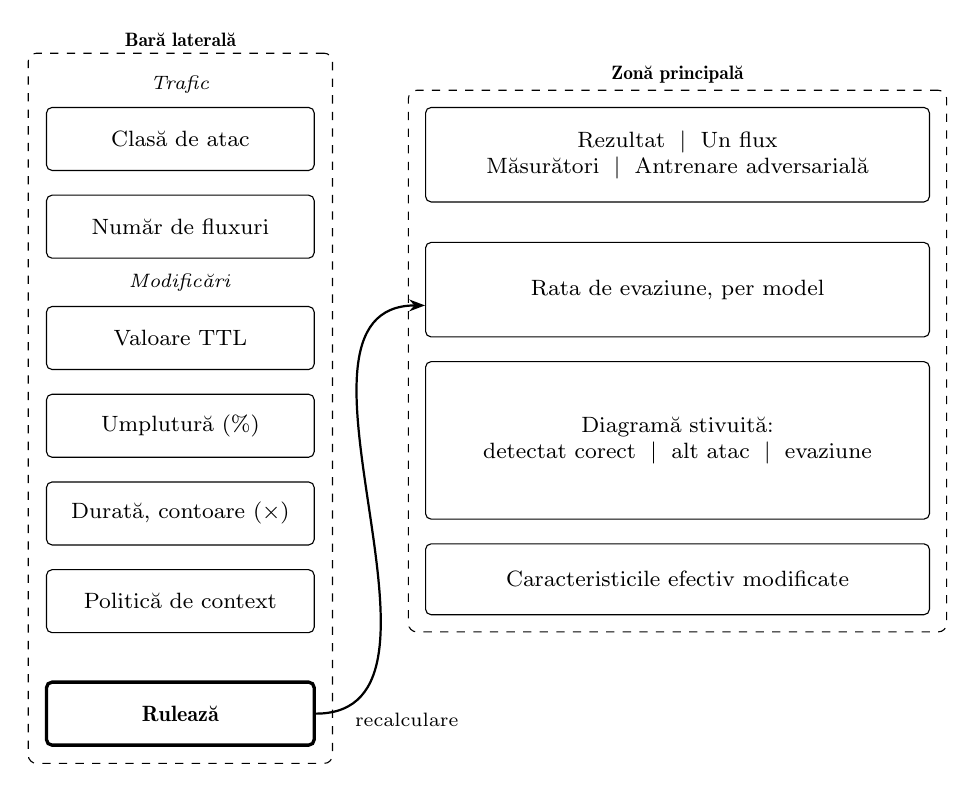
\begin{tikzpicture}[node distance=3mm and 6mm]
        \node[bloc, minimum width=34mm, minimum height=8mm] (t1) {Clasă de atac};
        \node[bloc, minimum width=34mm, minimum height=8mm, below=of t1] (t2) {Număr de fluxuri};
        \node[bloc, minimum width=34mm, minimum height=8mm, below=6mm of t2] (m1) {Valoare TTL};
        \node[bloc, minimum width=34mm, minimum height=8mm, below=of m1] (m2) {Umplutură (\%)};
        \node[bloc, minimum width=34mm, minimum height=8mm, below=of m2] (m3) {Durată, contoare ($\times$)};
        \node[bloc, minimum width=34mm, minimum height=8mm, below=of m3] (m4) {Politică de context};
        \node[bloc, minimum width=34mm, minimum height=8mm, below=6mm of m4, very thick] (run) {\textbf{Rulează}};

        \node[eticheta, above=1mm of t1] (lt) {\textit{Trafic}};
        \node[eticheta] at ($(t2.south)!0.5!(m1.north)$) {\textit{Modificări}};

        \node[bloc, minimum width=64mm, minimum height=12mm, right=14mm of t1.north east, anchor=north west]
            (file) {Rezultat \;$\vert$\; Un flux\\ Măsurători \;$\vert$\; Antrenare adversarială};
        \node[bloc, minimum width=64mm, minimum height=12mm, below=5mm of file] (met)
            {Rata de evaziune, per model};
        \node[bloc, minimum width=64mm, minimum height=20mm, below=of met] (chart)
            {Diagramă stivuită:\\ detectat corect \;$\vert$\; alt atac \;$\vert$\; evaziune};
        \node[bloc, minimum width=64mm, minimum height=9mm, below=of chart] (chg)
            {Caracteristicile efectiv modificate};

        \draw[sageata] (run.east) to[out=0, in=180] node[eticheta, below right, pos=0.08] {recalculare} ($(met.west)+(0,-2mm)$);

        \begin{scope}[on background layer]
            \node[grup, fit=(lt)(t1)(m4)(run), label={[eticheta]above:\textbf{Bară laterală}}] {};
            \node[grup, fit=(file)(chg), label={[eticheta]above:\textbf{Zonă principală}}] {};
        \end{scope}
    \end{tikzpicture}
    \caption{Organizarea ecranului interfeței interactive. Nimic nu se recalculează până la acționarea butonului, astfel încât rezultatele afișate corespund întotdeauna ultimei rulări.}
    \label{fig:ecran}
\end{figure}

\subsection{Stabilirea parametrilor și rularea}\label{subsec:parametri}

Utilizatorul introduce valorile dorite în bara laterală, apoi apasă butonul de rulare. Până la apăsarea butonului nu se recalculează nimic: valorile afișate în zona principală corespund întotdeauna ultimei rulări, nu câmpurilor editate între timp. Sub titlu este afișat, într-un singur rând, rezumatul parametrilor efectiv aplicați, tocmai pentru ca o eventuală diferență față de câmpurile editate să fie vizibilă.

Controalele disponibile sunt următoarele:

\begin{description}[style=nextline]
    \item[Clasa de atac.] Selectează categoria de trafic malițios analizată sau, alternativ, toate categoriile.
    \item[Numărul de fluxuri.] Stabilește dimensiunea eșantionului asupra căruia se aplică perturbarea. Valorile mari cresc precizia estimării și timpul de calcul.
    \item[Valoarea TTL.] Valoarea către care este modificat TTL-ul pachetelor emise. Poate fi dezactivată complet.
    \item[Umplutura.] Procentul de octeți adăugați la volumul transmis.
    \item[Factorul de durată.] Multiplicatorul aplicat duratei fluxului.
    \item[Factorul contoarelor.] Multiplicatorul aplicat contoarelor de conexiuni. Valorile subunitare corespund unei încetiniri a atacului.
    \item[Politica de context.] Selectează una dintre cele două ipoteze descrise în subsecțiunea~\ref{subsec:interval}.
\end{description}

Spre deosebire de experimentele sistematice, care folosesc un set predefinit de niveluri, interfața acceptă valori arbitrare în limitele fizic admisibile.

\subsection{Interpretarea rezultatelor}\label{subsec:interpretare}

Fila \textit{Rezultat} afișează, pentru fiecare dintre cele trei modele, rata de evaziune obținută și numărul de fluxuri eligibile care au intrat în calcul. Sub acestea, o diagramă cu bare orizontale prezintă distribuția celor trei rezultate posibile, folosind un cod de culoare constant: verde pentru fluxurile detectate corect, galben pentru cele confundate cu alt tip de atac și roșu pentru evaziune. Un rând final indică ce caracteristici au fost efectiv modificate de configurația curentă.

Fila \textit{Un flux} permite inspectarea unui singur flux, selectat prin index. Sunt afișate identificatorul și eticheta reală, tabelul valorilor modificate, cu valoarea dinainte și cea de după, și, pentru fiecare model, tranziția de la predicția pe traficul nemodificat la cea pe varianta perturbată, colorată conform aceluiași cod. Această vedere este utilă pentru a înțelege concret ce anume se schimbă într-un flux și cum reacționează fiecare model.

Fila \textit{Măsurători} prezintă tabelele și figurile obținute în urma rulărilor sistematice, pentru comparație cu rezultatele explorate interactiv.

Rezultatele reantrenării, discutate în secțiunea~\ref{sec:rezultate-o6}, sunt prezentate în ultima filă. Pentru fiecare model și fiecare grup sunt afișate macro-$F1$ pe traficul nemodificat și rata de evaziune în cel mai rău caz, împreună cu varianta care o produce și cu dimensiunea mulțimii comune pe care s-a măsurat. Un selector permite alegerea modelului pentru care se afișează confruntarea cu criteriile stabilite înaintea rulării.

\subsection{Situații speciale}\label{subsec:situatii}

Dacă o combinație de parametri produce o variantă care încalcă o constrângere de validitate, interfața afișează un mesaj de eroare care indică verificarea încălcată, în locul unei rate de evaziune. Comportamentul este intenționat: un rezultat obținut pentru un flux imposibil fizic ar fi lipsit de semnificație.

Dacă selecția nu conține niciun flux eligibil, situație posibilă la eșantioane foarte mici din clase rare, se afișează un avertisment corespunzător, întrucât rata de evaziune nu este definită pe o mulțime vidă.

Dacă fila \textit{Măsurători} sau fila \textit{Antrenare adversarială} indică absența rezultatelor, etapele sistematice corespunzătoare din tabelul~\ref{tab:rulare} nu au fost încă executate. Fiecare filă semnalează separat această situație, iar restul interfeței rămâne funcțional, întrucât explorarea live nu depinde de aceste etape.
 % \chapter{Manual de Instalare și Utilizare}

\chapter{Concluzii}\label{ch:concluzii}
\pagestyle{fancy}

\section{Contribuții}\label{sec:contributii}

Lucrarea a evaluat empiric robustețea a trei clasificatoare de trafic de rețea în fața unor modificări adversariale realizabile, folosind setul de date UNSW-NB15. Contribuțiile pot fi grupate în trei categorii.

\textbf{Contribuții metodologice.} A fost formulată o mulțime de perturbări admisibile care înlocuiește limita de distanță folosită de obicei în literatura exemplelor adversariale cu o mulțime structurată, definită prin patru condiții: direcționalitate, limite relative la observația originală, imuabilitatea caracteristicilor aflate în afara controlului atacatorului și închiderea la relațiile de dependență dintre caracteristici. Ultima condiție a necesitat un mecanism propriu de propagare, enunțat în subsecțiunea~\ref{subsec:propagare}, care recalculează exact caracteristicile derivate fără a cunoaște constantele senzorului care a produs datele și fără a altera valorile originale. A fost tratată explicit situația unei caracteristici care nu poate fi reconstituită din înregistrări izolate, prin raportarea rezultatului sub formă de interval delimitat de două ipoteze declarate, în locul unei valori unice obținute printr-o presupunere nedeclarată. Pentru partea de apărare a fost formulat un protocol experimental care separă efectul perturbării de cel al volumului suplimentar de date, prin introducerea unui grup de control antrenat pe același număr de exemple neperturbate, prin înghețarea ponderilor de clasă la valorile calculate pe setul original și prin raportarea ratelor pe o mulțime de fluxuri fixată în prealabil, comună tuturor variantelor comparate. Criteriile de succes au fost consemnate înaintea rulării, iar rezultatul este raportat inclusiv acolo unde ele nu au fost îndeplinite.

\textbf{Contribuții experimentale.} Au fost antrenate și evaluate comparativ trei modele cu predispoziții inductive diferite, două ansambluri de arbori și o arhitectură bazată pe atenție implementată de la zero, iar ratele lor de evaziune au fost măsurate sub 28 de variante de perturbare. Analiza de sensibilitate a legat cantitativ rezistența fiecărui model de distribuția importanței caracteristicilor sale, prin introducerea unei mărimi care exprimă ce fracțiune din capacitatea de detecție a unui model se află efectiv la îndemâna atacatorului. Cele trei modele au fost apoi reantrenate pe date augmentate cu variante perturbate și reevaluate în aceleași condiții, alături de un grup de control și de un grup antrenat cu o familie de transformări exclusă deliberat, care măsoară dacă robustețea obținută se transferă la modificări nevăzute la antrenare.

\textbf{Contribuții practice.} A fost realizată o interfață care permite explorarea interactivă a comportamentului modelelor sub perturbări cu parametri arbitrari, construită astfel încât să compună aceleași primitive validate ca experimentele sistematice, nu o implementare paralelă a acestora.

\section{Analiza critică a rezultatelor}\label{sec:critica}

Rezultatul principal este că o singură modificare a valorii TTL, realizabilă prin configurarea socketului, restrânsă la valori compatibile cu păstrarea funcționalității atacului în modelul de amenințare adoptat și fără nicio cunoaștere a sistemului de detecție, duce modelul cu cel mai mare macro-$F1$ pe traficul nemodificat de la $0\%$ la peste $50\%$ evaziune. Realizabilitatea acestei modificări este argumentată în cadrul experimental adoptat, nu demonstrată prin generarea și retransmiterea traficului real, conform limitării enunțate în secțiunea~\ref{sec:limitari}. Combinată cu umplutură și dilatare temporală, rata ajunge la aproape $97\%$. Celelalte transformări analizate lasă evaziunea sub $1{,}3\%$ la orice intensitate.

Reantrenarea pe trafic perturbat elimină aproape complet această vulnerabilitate: evaziunea în cel mai rău caz scade sub $0{,}5\%$ la toate cele trei modele, iar câștigul se menține și față de grupul de control, deci nu provine din volumul suplimentar de date. Costul este modest pe metricile globale, sub $0{,}023$ de macro-$F1$, dar concentrat: clasa cea mai rară pierde între $0{,}075$ și $0{,}127$, ceea ce o metrică agregată ar fi ascuns.

Trei constatări merită subliniate pentru că nuanțează concluzii care altfel ar fi fost formulate greșit.

Prima privește relația dintre acuratețe și robustețe. Modelul cu cele mai bune metrici pe trafic nemodificat este și cel mai fragil sub perturbare, iar analiza importanței prin permutare oferă o explicație plauzibilă: $54{,}6\%$ din scăderea totală a ratei de detecție măsurată astfel se concentrează într-o singură caracteristică. Rezultă că evaluarea exclusiv pe trafic nemodificat nu este suficientă pentru caracterizarea comportamentului adversarial, iar selecția unui model pe baza acuratețeii poate conduce la alegerea celui mai vulnerabil.

A doua privește interpretarea rezistenței observate. Transformer cedează cel mai puțin la perturbările realizabile, dar analiza de sensibilitate sugerează că această rezistență este explicată în mare măsură de dependența de caracteristici aflate în afara controlului atacatorului: doar $26{,}0\%$ din capacitatea sa de detecție îi este accesibilă, iar caracteristica pe care se sprijină preponderent este generată de victimă. Atunci când constrângerea de accesibilitate este relaxată artificial, rata sa de evaziune urcă la $71{,}1\%$. Ceea ce s-ar fi putut raporta drept robustețe arhitecturală se explică, prin urmare, în bună măsură printr-o particularitate a datelor. O evaluare bazată exclusiv pe ratele de evaziune, fără analiza de sensibilitate, ar fi condus la recomandarea eronată de a prefera această arhitectură.

A treia privește interpretarea apărării. Ratele apropiate de zero obținute după reantrenare se referă la exact familia de transformări folosită la antrenare, iar întrebarea dacă modelul a învățat proprietatea care face aceste transformări eficiente sau doar transformările înseși nu poate fi decisă măsurând pe ele. Grupul antrenat cu familia TTL exclusă și măsurat tocmai pe ea răspunde direct: Random Forest coboară de la $80{,}3\%$ la $11{,}8\%$ pe transformări pe care nu le-a văzut niciodată, în timp ce celelalte două modele rămân practic neschimbate, iar unul dintre ele devine chiar mai vulnerabil pe două variante. Invarianța învățată se transferă, prin urmare, doar la unul dintre cele trei modele. Fără acest grup, rezultatul ar fi fost raportat ca robustețe generală la perturbări realizabile, ceea ce datele nu susțin.

\section{Limitări}\label{sec:limitari}

Rezultatele trebuie interpretate în limitele următoare.

\textbf{Un singur set de date.} Toate concluziile sunt obținute pe UNSW-NB15. Constatarea că valoarea TTL funcționează ca artefact al mediului de captură este specifică acestui set. Ea sugerează însă că verificarea existenței unor artefacte similare ar trebui să preceadă orice evaluare de robustețe pe alt set. Tot de partiția oficială ține și nivelul ridicat al alarmelor false pe traficul legitim, între $24{,}4\%$ și $41{,}4\%$, discutat în subsecțiunea~\ref{subsec:semnalare}: cele două jumătăți ale partiției nu au aceeași distribuție, iar la testare modelele întâlnesc de două ori mai mult trafic legitim purtând semnătura TTL învățată ca indiciu de atac. Aceste valori nu afectează concluziile privind evaziunea, care se sprijină exclusiv pe rata de semnalare a atacurilor, dar limitează orice afirmație despre utilitatea operațională a modelelor.

\textbf{Perturbări în spațiul caracteristicilor.} Modificările sunt aplicate reprezentării tabelare, cu argumentarea că fiecare corespunde unei acțiuni realizabile asupra traficului. Validarea completă ar presupune generarea traficului modificat, trecerea lui printr-un senzor real și compararea caracteristicilor rezultate cu cele calculate prin propagare.

\textbf{Atacator neadaptiv.} Modelul de amenințare exclude interogarea sistemului de detecție. Un atacator cu acces la răspunsurile modelului ar obține rezultate cel puțin la fel de bune, deci valorile raportate constituie estimări conservatoare.

\textbf{Contorul de context nereconstituibil.} Pentru transformările care implică valori TTL, rezultatul este un interval, uneori larg. Determinarea valorii reale ar necesita datele de flux brute, cu contextul temporal al fiecărei conexiuni.

\textbf{O singură rundă a interacțiunii atac-apărare.} Apărarea evaluată presupune că atacatorul își păstrează transformările neschimbate după reantrenare. Un atacator care ar observa modelul apărat și și-ar reoptimiza modificările împotriva lui rămâne în afara cadrului: rezultatele descriu o rundă a acestei interacțiuni, nu punctul ei de echilibru.

\textbf{Robustețe limitată la familia de transformări cunoscută.} Grupul antrenat cu familia TTL exclusă arată că invarianța învățată se transferă la transformări nevăzute doar pentru unul dintre cele trei modele. Pentru celelalte două, valorile apropiate de zero obținute pe familia cunoscută nu pot fi extinse la perturbări realizabile în general. Măsurarea acestei limite a fost posibilă doar pentru că o familie a fost exclusă deliberat. Un experiment fără acest grup ar fi raportat o robustețe pe care rezultatele nu o susțin.

\section{Dezvoltări ulterioare}\label{sec:dezvoltari}

Direcțiile de continuare decurg direct din limitările enumerate.

\textbf{Validarea la nivel de trafic.} Reconstruirea perturbărilor asupra fișierelor de captură brute și trecerea lor printr-un senzor real ar transforma argumentul de realizabilitate din unul deductiv în unul verificat experimental. Este cea mai valoroasă continuare, întrucât adresează limitarea cea mai importantă.

\textbf{Extinderea la alte seturi de date.} Repetarea experimentului pe seturi produse în medii de captură diferite ar permite distincția între vulnerabilitățile datorate arhitecturii modelului și cele datorate particularităților unui set anume.

\textbf{Atacuri adaptive.} Modelul Transformer este diferențiabil de la un capăt la altul, ceea ce permite, spre deosebire de ansamblurile de arbori, aplicarea metodelor bazate pe gradient. Compararea rezultatelor acestora cu perturbările structurate din prezenta lucrare ar arăta cât din diferență provine din puterea metodei și cât din relaxarea constrângerilor de realizabilitate.

\textbf{Atacatori adaptivi împotriva modelului apărat.} Continuarea imediată a părții de apărare este a doua rundă a interacțiunii: generarea de transformări optimizate împotriva modelului reantrenat, urmată de o nouă reantrenare. Rezultatul relevant nu este rata de evaziune la o rundă anume, ci dacă succesiunea converge sau oscilează.

\textbf{Recuperarea claselor rare.} Degradarea clasei celei mai rare este cel mai clar cost al procedurii actuale. Direcțiile evidente sunt augmentarea diferențiată, care să adauge copii perturbate proporțional cu fragilitatea fiecărei clase în loc de uniform, și recalcularea ponderilor de clasă pe numărătorile augmentate. Această a doua direcție a fost exclusă aici deliberat, pentru comparabilitatea funcției de cost, dar devine rezonabilă odată ce comparația controlată a fost făcută.

\textbf{Alte mecanisme de apărare.} Cadrul de măsurare rămâne direct reutilizabil pentru contramăsuri de alt tip: eliminarea deliberată a caracteristicilor identificate ca artefacte sau regularizarea care descurajează concentrarea deciziei într-o singură caracteristică. Mărimea introdusă în subsecțiunea~\ref{subsec:accesibila} poate servi în acest context drept criteriu de proiectare, nu doar de diagnostic: un model proiectat astfel încât să reducă dependența de caracteristici ușor controlabile de atacator ar putea prezenta o robustețe mai bună față de familia de perturbări analizată.

\textbf{Selecția caracteristicilor orientată către robustețe.} Rezultatele sugerează că excluderea deliberată a caracteristicilor ușor de manipulat ar putea reduce acuratețea pe trafic nemodificat, dar crește robustețea. Cuantificarea acestui compromis constituie o direcție de cercetare distinctă.
 % \chapter{Concluzii}

% Bibliografie — format IEEE (thebibliography)
% Cheile corespund comenzilor \cite din capitole.
% Ordinea: seturi de date [1-5], modele de clasificare [6-10],
%          rețele neuronale și transformere [11-16], ML adversarial și evaziune [17-25].

\begin{thebibliography}{25}

% ---------- Seturi de date ----------

\bibitem{ring2019survey}
M.~Ring, S.~Wunderlich, D.~Scheuring, D.~Landes, and A.~Hotho, ``A survey of network-based intrusion detection data sets,'' \textit{Computers \& Security}, vol.~86, 2019.

\bibitem{moustafa2015unsw}
N.~Moustafa and J.~Slay, ``UNSW-NB15: A comprehensive data set for network intrusion detection systems (UNSW-NB15 network data set),'' in \textit{Proc. Military Communications and Information Systems Conference (MilCIS)}, Canberra, Australia, 2015.

\bibitem{sharafaldin2018cicids}
I.~Sharafaldin, A.~Habibi~Lashkari, and A.~A. Ghorbani, ``Toward generating a new intrusion detection dataset and intrusion traffic characterization,'' in \textit{Proc. 4th Int. Conf. on Information Systems Security and Privacy (ICISSP)}, Funchal, Portugal, 2018.

\bibitem{tavallaee2009kdd}
M.~Tavallaee, E.~Bagheri, W.~Lu, and A.~A. Ghorbani, ``A detailed analysis of the KDD CUP 99 data set,'' in \textit{Proc. IEEE Symp. Computational Intelligence for Security and Defense Applications (CISDA)}, 2009.

\bibitem{liu2022error}
L.~Liu, G.~Engelen, T.~Lynar, D.~Essam, and W.~Joosen, ``Error prevalence in NIDS datasets: A case study on CIC-IDS-2017 and CSE-CIC-IDS-2018,'' in \textit{Proc. IEEE Conf. on Communications and Network Security (CNS)}, 2022.

% ---------- Modele de clasificare ----------

\bibitem{breiman2001random}
L.~Breiman, ``Random forests,'' \textit{Machine Learning}, vol.~45, no.~1, pp.~5--32, 2001.

\bibitem{chen2016xgboost}
T.~Chen and C.~Guestrin, ``XGBoost: A scalable tree boosting system,'' in \textit{Proc. 22nd ACM SIGKDD Int. Conf. on Knowledge Discovery and Data Mining}, San Francisco, CA, USA, 2016, pp.~785--794.

\bibitem{uddin2024hierarchical}
M.~A. Uddin, S.~Aryal, M.~R. Bouadjenek, M.~Al-Hawawreh, and M.~A. Talukder, ``Hierarchical classification for intrusion detection system: Effective design and empirical analysis,'' \textit{Ad Hoc Networks}, 2025.
% TODO: articolul a fost publicat în Ad Hoc Networks (Elsevier, 2025, open access).
% Completează volumul și numărul de articol de pe ScienceDirect:
% https://www.sciencedirect.com/science/article/pii/S1570870525002306

\bibitem{alhameed2025enhancing}
A.~A. Alhameed, A.~A. Hadi, and W.~H. Al-Masoody, ``Enhancing network security: A study on classification models for intrusion detection systems,'' \textit{Journal of Communications Software and Systems}, vol.~21, no.~2, 2025.

\bibitem{agarwal2021classification}
A.~Agarwal, P.~Sharma, M.~Alshehri, A.~A. Mohamed, and O.~Alfarraj, ``Classification model for accuracy and intrusion detection using machine learning approach,'' \textit{PeerJ Computer Science}, vol.~7, 2021.

% ---------- Rețele neuronale și transformere pentru detecția intruziunilor ----------

\bibitem{vaswani2017attention}
A.~Vaswani, N.~Shazeer, N.~Parmar, J.~Uszkoreit, L.~Jones, A.~N. Gomez, {\L}.~Kaiser, and I.~Polosukhin, ``Attention is all you need,'' in \textit{Advances in Neural Information Processing Systems (NeurIPS)}, vol.~30, 2017.

\bibitem{gorishniy2021revisiting}
Y.~Gorishniy, I.~Rubachev, V.~Khrulkov, and A.~Babenko, ``Revisiting deep learning models for tabular data,'' in \textit{Advances in Neural Information Processing Systems (NeurIPS)}, vol.~34, 2021.

\bibitem{wu2022rtids}
Z.~Wu, H.~Zhang, P.~Wang, and Z.~Sun, ``RTIDS: A robust transformer-based approach for intrusion detection system,'' \textit{IEEE Access}, vol.~10, 2022.

\bibitem{manocchio2024flowtransformer}
L.~D. Manocchio, S.~Layeghy, W.~W. Lo, G.~K. Kulatilleke, M.~Sarhan, and M.~Portmann, ``FlowTransformer: A transformer framework for flow-based network intrusion detection systems,'' \textit{Expert Systems with Applications}, vol.~241, art.~122564, 2024.

\bibitem{ullah2024idsint}
F.~Ullah, S.~Ullah, G.~Srivastava, and J.~C.-W. Lin, ``IDS-INT: Intrusion detection system using transformer-based transfer learning for imbalanced network traffic,'' \textit{Digital Communications and Networks}, vol.~10, no.~1, 2024.

\bibitem{zhang2022adversarial}
C.~Zhang, X.~Costa-P\'erez, and P.~Patras, ``Adversarial attacks against deep learning-based network intrusion detection systems and defense mechanisms,'' \textit{IEEE/ACM Transactions on Networking}, vol.~30, no.~3, 2022.

% ---------- Învățare automată adversarială și evaziune ----------

\bibitem{he2023adversarial}
K.~He, D.~D. Kim, and M.~R. Asghar, ``Adversarial machine learning for network intrusion detection systems: A comprehensive survey,'' \textit{IEEE Communications Surveys \& Tutorials}, vol.~25, no.~1, 2023.

\bibitem{szegedy2014intriguing}
C.~Szegedy, W.~Zaremba, I.~Sutskever, J.~Bruna, D.~Erhan, I.~J. Goodfellow, and R.~Fergus, ``Intriguing properties of neural networks,'' in \textit{Proc. Int. Conf. on Learning Representations (ICLR)}, 2014.

\bibitem{goodfellow2015explaining}
I.~J. Goodfellow, J.~Shlens, and C.~Szegedy, ``Explaining and harnessing adversarial examples,'' in \textit{Proc. Int. Conf. on Learning Representations (ICLR)}, 2015.

\bibitem{madry2018towards}
A.~Madry, A.~Makelov, L.~Schmidt, D.~Tsipras, and A.~Vladu, ``Towards deep learning models resistant to adversarial attacks,'' in \textit{Proc. Int. Conf. on Learning Representations (ICLR)}, 2018.

\bibitem{alotaibi2023adversarial}
A.~Alotaibi and M.~A. Rassam, ``Adversarial machine learning attacks against intrusion detection systems: A survey on strategies and defense,'' \textit{Future Internet}, vol.~15, no.~2, art.~62, 2023.

\bibitem{sharon2022tantra}
Y.~Sharon, D.~Berend, Y.~Liu, A.~Shabtai, and Y.~Elovici, ``TANTRA: Timing-based adversarial network traffic reshaping attack,'' \textit{IEEE Transactions on Information Forensics and Security}, vol.~17, 2022.

\bibitem{tan2022sneaking}
S.~Tan, X.~Zhong, Z.~Tian, and Q.~Dong, ``Sneaking through security: Mutating live network traffic to evade learning-based NIDS,'' \textit{IEEE Transactions on Network and Service Management}, vol.~19, no.~3, 2022.



\bibitem{gont2011rfc6274}
F.~Gont, ``Security assessment of the Internet Protocol version 4,'' Internet Engineering Task Force, RFC~6274, Jul.~2011.

\bibitem{okada2025xai}
S.~Okada, H.~Jmila, K.~Akashi, T.~Mitsunaga, Y.~Sekiya, H.~Takase, G.~Blanc, and H.~Nakamura, ``XAI-driven black-box adversarial attacks on network intrusion detectors,'' \textit{International Journal of Information Security}, vol.~24, no.~3, art.~103, 2025.

\end{thebibliography}
 % Bibliografie — thebibliography manual, format IEEE

\appendix
\chapter{Secțiuni relevante din cod}\label{ch:anexa-cod}
\pagestyle{fancy}

Anexa reproduce fragmentele de cod la care se face referire în capitolele~\ref{ch:analysis} și \ref{ch:proiectare}, alese pentru că implementează direct rezultatele formulate teoretic. Primele șase secțiuni acoperă cei patru algoritmi din secțiunea~\ref{sec:algoritmi}: generarea unei variante și cele două proceduri pe care le apelează, măsurarea evaziunii împreună cu taxonomia rezultatelor și determinarea importanței determinate prin permutare. Comentariile din cod sunt redate ca atare.

\section{Generarea unei variante perturbate}\label{sec:anexa-generare}

Fragmentul implementează Algoritmul~\ref{alg:generare}. Funcția orchestrează pașii, delegând transformarea propriu-zisă generatorului corespunzător tipului cerut. Propagarea și rezolvarea contorului se produc în interiorul acestuia, iar restaurarea tipurilor încheie procedura. Un nivel în afara intervalului admis produce o eroare, nu o valoare limitată tacit.

\begin{verbatim}
def generate_variant(X, perturbation_type, level, ctx):
    """Genereaza o singura varianta perturbata."""
    if perturbation_type not in PERTURBATION_TYPES:
        raise ValueError(
            f"tip de perturbare necunoscut: {perturbation_type!r}")
    func, n_levels, _ = PERTURBATION_TYPES[perturbation_type]

    # Nivelul 0 e identitatea, folosita drept control: predictiile
    # pe ea trebuie sa reproduca exact baseline-ul.
    if level == 0:
        return identity(X, 0, ctx)
    if not 1 <= level <= n_levels:
        raise ValueError(f"nivel {level} invalid pentru "
                         f"{perturbation_type!r} (1..{n_levels})")

    perturbed, meta = func(X, level, ctx)
    # Propagarea si rezolvarea contorului se fac in `func`; aici se
    # readuc doar tipurile pe care modelul inghetat le asteapta.
    return schema.restore_dtypes(perturbed, X), meta
\end{verbatim}


\section{Propagarea dependențelor}\label{sec:anexa-propagare}

Fragmentul implementează observația centrală din subsecțiunea~\ref{subsec:propagare}. Rapoartele se calculează față de valorile originale, iar caracteristicile derivate se obțin prin înmulțire, nu prin recalculare din formula senzorului. Funcția auxiliară \verb|_safe_ratio| tratează numitorii nuli prin raportul neutru, lăsând caracteristica derivată neschimbată.

\begin{verbatim}
NEUTRAL_RATIO = 1.0

def _safe_ratio(new_values, old_values) -> np.ndarray:
    """Raport element-cu-element, 1.0 unde numitorul e 0."""
    new_arr = np.asarray(new_values, dtype=float)
    old_arr = np.asarray(old_values, dtype=float)
    ratio = np.divide(new_arr, old_arr,
                      out=np.full_like(old_arr, NEUTRAL_RATIO),
                      where=old_arr != 0)
    return np.where(np.isfinite(ratio), ratio, NEUTRAL_RATIO)


def propagate(original, perturbed):
    """Recalculeaza derivatele dupa o schimbare de baza."""
    out = perturbed.copy()

    r_bytes = _safe_ratio(out.sbytes, original.sbytes)
    r_pkts  = _safe_ratio(out.spkts, original.spkts)
    r_dur   = _safe_ratio(out.dur, original.dur)
    # rate ~ (spkts + dpkts - 1) / dur ; dpkts nu se modifica
    r_pktsum = _safe_ratio(out.spkts + out.dpkts - 1,
                           original.spkts + original.dpkts - 1)
    # sinpkt ~ dur / (spkts - 1) : numarul de intervale
    r_gaps = _safe_ratio(out.spkts - 1, original.spkts - 1)

    out["smean"]  = original.smean  * r_bytes / r_pkts
    out["sload"]  = original.sload  * r_bytes / r_dur
    out["rate"]   = original["rate"] * r_pktsum / r_dur
    out["sinpkt"] = original.sinpkt * r_dur / r_gaps
    out["sjit"]   = original.sjit   * r_dur

    # Antrenate cauzal de dilatarea duratei: daca atacatorul
    # intarzie, raspunsurile victimei se intind si ele in timp.
    out["dload"]  = original.dload  / r_dur
    out["dinpkt"] = original.dinpkt * r_dur
    out["djit"]   = original.djit   * r_dur
    return out, stats
\end{verbatim}

\section{Rezolvarea contorului de context}\label{sec:anexa-ct}

Fragmentul materializează cele două politici din subsecțiunea~\ref{subsec:interval}. Politica conservatoare returnează valoarea originală fără a consulta vreo corespondență, iar cea optimistă încearcă, în ordine, tripletul exact observat în date, semnătura traficului legitim pentru aceeași valoare TTL și, în ultimă instanță, o constantă declarată explicit. Statisticile returnate permit raportarea, în fișa rulării, a numărului de rânduri rezolvate pe fiecare cale.

\begin{verbatim}
def resolve_ct_state_ttl(perturbed, policy, lookup, normal_lookup):
    """Determina ct_state_ttl cand sttl/dttl s-au schimbat.

    ct_state_ttl NU e o functie de intervale TTL (sttl=62 -> 2, dar
    sttl=63 -> 0), ci un contor pe fereastra glisanta de 100 de
    conexiuni, imposibil de recalculat din inregistrari izolate.
    """
    if policy not in config.CT_STATE_TTL_POLICIES:
        raise ValueError(
            f"politica ct_state_ttl necunoscuta: {policy!r}")

    if policy == "hold":
        return perturbed["ct_state_ttl"], {...}

    keys = pd.MultiIndex.from_arrays(
        [perturbed["state"], perturbed["sttl"], perturbed["dttl"]])
    exact = lookup.reindex(keys)
    exact_hit = exact.notna().to_numpy()

    from_normal = normal_lookup.reindex(
        perturbed["sttl"]).to_numpy(dtype=float)
    normal_hit = ~np.isnan(from_normal) & ~exact_hit

    values = np.where(exact_hit, exact.to_numpy(dtype=float),
                      np.where(normal_hit, from_normal,
                               config.CT_STATE_TTL_FALLBACK))
    return pd.Series(values, index=perturbed.index), stats
\end{verbatim}

\section{Măsurarea evaziunii pe o variantă}\label{sec:anexa-masurare}

Fragmentul implementează pașii 3--5 din Algoritmul~\ref{alg:masurare}. Varianta nu este citită de pe disc, ci regenerată în memorie, generarea fiind deterministă. Restrângerea la fluxurile eligibile se aplică înaintea oricărei numărători, conform criteriului din subsecțiunea~\ref{subsec:eligibil}.

\begin{verbatim}
def measure_variant(models, references, X, true_labels, ids,
                    variant_type, level, ctx):
    """Masoara o varianta, pentru toate modelele."""
    variant, _ = generators.generate_variant(
        X, variant_type, level, ctx)

    summaries = []
    for model_name, model in models.items():
        reference = references[model_name]
        mask = reference["eligible"]

        predictions = model.predict(variant)

        # Totul se restrange la fluxurile ELIGIBILE: cele pe care
        # modelul le-a semnalat deja pe traficul nemodificat.
        eligible_true = true_labels[mask]
        eligible_pred = np.asarray(predictions)[mask]
        row_outcomes = outcome_utils.classify_outcomes(
            eligible_true, eligible_pred)

        summary = outcome_utils.evasion_summary(row_outcomes)
        summary.update({"model": model_name,
                        "type": variant_type, "level": level})
        summaries.append(summary)
    return summaries
\end{verbatim}


\section{Taxonomia celor trei rezultate}\label{sec:anexa-outcomes}

Fragmentul implementează literal cele trei rezultate din subsecțiunea~\ref{subsec:rezultate}. Ordinea atribuirilor contează: eticheta implicită este confuzia cu alt tip de atac, peste care se suprascriu întâi evaziunea, apoi clasificarea corectă.

\begin{verbatim}
def classify_outcomes(true_labels, predictions) -> np.ndarray:
    """Incadreaza fiecare flux perturbat in una dintre cele
    trei categorii."""
    true_arr = np.asarray(true_labels)
    pred_arr = np.asarray(predictions)

    outcomes = np.full(len(pred_arr),
                  config.OUTCOME_MISCLASSIFIED_ATTACK, dtype=object)
    outcomes[pred_arr == "Normal"] = config.OUTCOME_EVADED
    outcomes[(pred_arr == true_arr)
             & (pred_arr != "Normal")] = config.OUTCOME_CORRECT
    return outcomes
\end{verbatim}

\section{Importanța prin permutare}\label{sec:anexa-importanta-cod}

Fragmentul implementează pașii 1--3 din Algoritmul~\ref{alg:sensibilitate}. Parametrul \verb|donor| materializează corecția discutată în subsecțiunea~\ref{subsec:alg-sensibilitate}: fără el, o analiză restrânsă la o singură clasă ar raporta importanță nulă pentru caracteristici cvasi-constante în acea clasă, deși modelul se poate sprijini decisiv pe ele.

\begin{verbatim}
def permutation_importance(model, X, y_true, columns=None,
                           n_repeats=5, seed=42, donor=None):
    """Importanta prin permutare, pe un model inghetat.

    DONOR: daca analiza e restransa la o clasa in care coloana e
    cvasi-constanta (in Generic, sttl e 254 la 98,8% din randuri),
    amestecarea interna nu schimba nimic si importanta iese fals
    ~0. Cu donor, valorile de inlocuire vin din alta distributie.
    """
    columns = list(columns or X.columns)
    is_attack = y_true != "Normal"
    base_detection, _ = _score(model.predict(X), y_true, is_attack)

    rows = []
    for index, column in enumerate(columns):
        drops = []
        for repeat in range(n_repeats):
            rng = np.random.default_rng(
                seed + 1000 * index + repeat)
            shuffled = X.copy()
            if donor is None:
                shuffled[column] = X[column].to_numpy()[
                    rng.permutation(len(X))]
            else:
                pool = donor[column].to_numpy()
                shuffled[column] = pool[
                    rng.integers(0, len(pool), size=len(X))]
            detection, _ = _score(model.predict(shuffled),
                                  y_true, is_attack)
            drops.append(base_detection - detection)

        rows.append({"feature": column,
                     "detection_drop": float(np.mean(drops)),
                     "detection_drop_std": float(np.std(drops))})

    return pd.DataFrame(rows).sort_values(
        "detection_drop", ascending=False)
\end{verbatim}


\section{Mecanismul de atenție}\label{sec:anexa-atentie}

Fragmentul implementează mecanismul de atenție descris în subsecțiunea~\ref{subsec:atentie}. Atenția este scrisă explicit, fără a folosi componente de nivel înalt din biblioteca de învățare profundă, pentru ca fiecare operație să fie verificabilă. Parametrul \verb|return_attention| expune ponderile, utile pentru interpretabilitate.

\begin{verbatim}
class MultiHeadSelfAttention(nn.Module):
    """Self-attention multi-head, scrisa explicit.

    Pentru fiecare cap h:
        Attention(Q,K,V) = softmax(Q K^T / sqrt(d_head)) V.
    Capetele sunt concatenate si proiectate inapoi in d_token.
    """

    def _split_heads(self, x):
        """[batch, tokens, d] -> [batch, n_heads, tokens, d_head]."""
        batch, tokens, _ = x.shape
        return x.view(batch, tokens,
                      self.n_heads, self.d_head).transpose(1, 2)

    def forward(self, x, return_attention: bool = False):
        q = self._split_heads(self.query(x))
        k = self._split_heads(self.key(x))
        v = self._split_heads(self.value(x))

        scores = q @ k.transpose(-2, -1) / math.sqrt(self.d_head)
        weights = self.dropout(F.softmax(scores, dim=-1))

        context = (weights @ v).transpose(1, 2).reshape(x.shape)
        out = self.projection(context)
        return (out, weights) if return_attention else out
\end{verbatim}

\chapter{Rezultate detaliate}\label{ch:anexa-rezultate}

Anexa conține rezultatele complete din care au fost extrase valorile sintetizate în capitolul~\ref{ch:testare}. Ele sunt reproduse integral pentru ca cifrele raportate în text să poată fi verificate în context.

\section{Rezultatele complete ale măsurării evaziunii}\label{sec:anexa-evaziune}

Tabelul~\ref{tab:anexa-evaziune} prezintă rata de evaziune pentru fiecare dintre cele 28 de variante generate. Capitolul~\ref{ch:testare} raportează doar valorile la intensitate maximă pentru fiecare tip de transformare. Se observă aici comportamentul nemonoton descris în subsecțiunea~\ref{subsec:nemonoton}: pentru transformările TTL, nivelul 2 produce sistematic o rată inferioară nivelului 1, deoarece nivelurile reprezintă valori-țintă distincte, nu intensități crescătoare. Varianta \verb|ttl_both| este marcată ca nerealizabilă și nu trebuie citită alături de celelalte.

\begin{table}[!ht]
    \caption{Rata de evaziune pentru toate cele 28 de variante (\% din fluxurile eligibile)}
    \centering\footnotesize
    \begin{tabular}{|l|c|c|c|c|}
        \hline
        \textbf{Tip} & \textbf{Nivel} & \textbf{RF} & \textbf{XGB} & \textbf{Transformer} \\
        \hline
        combined\_hold & 1 & 0,77 & 10,35 & 5,02 \\
        \hline
        combined\_hold & 2 & 0,80 & 5,17 & 7,12 \\
        \hline
        combined\_hold & 3 & 16,46 & 95,31 & 12,71 \\
        \hline
        combined\_hold & 4 & 31,31 & 96,44 & 17,42 \\
        \hline
        combined\_mimic & 1 & 9,92 & 46,78 & 46,16 \\
        \hline
        combined\_mimic & 2 & 0,81 & 5,15 & 7,35 \\
        \hline
        combined\_mimic & 3 & 66,37 & 96,17 & 66,89 \\
        \hline
        combined\_mimic & 4 & 75,89 & 96,92 & 71,02 \\
        \hline
        connection\_rate & 1 & 0,21 & 0,50 & 0,00 \\
        \hline
        connection\_rate & 2 & 0,20 & 0,56 & 0,00 \\
        \hline
        connection\_rate & 3 & 0,21 & 0,49 & 0,00 \\
        \hline
        connection\_rate & 4 & 0,33 & 0,33 & 0,00 \\
        \hline
        identity & 0 & 0,00 & 0,00 & 0,00 \\
        \hline
        padding & 1 & 0,15 & 1,23 & 0,10 \\
        \hline
        padding & 2 & 0,11 & 0,96 & 0,01 \\
        \hline
        padding & 3 & 0,12 & 0,99 & 0,02 \\
        \hline
        padding & 4 & 0,14 & 1,20 & 0,07 \\
        \hline
        timing & 1 & 0,23 & 0,60 & 0,01 \\
        \hline
        timing & 2 & 0,24 & 0,65 & 0,02 \\
        \hline
        timing & 3 & 0,42 & 0,86 & 0,02 \\
        \hline
        timing & 4 & 0,73 & 1,12 & 0,02 \\
        \hline
        ttl\_both & 1 & 33,02 & 51,07 & 71,07 \\
        \hline
        ttl\_hold & 1 & 0,49 & 7,59 & 3,17 \\
        \hline
        ttl\_hold & 2 & 0,49 & 6,51 & 3,21 \\
        \hline
        ttl\_hold & 3 & 4,44 & 50,21 & 4,04 \\
        \hline
        ttl\_mimic & 1 & 4,46 & 8,74 & 36,98 \\
        \hline
        ttl\_mimic & 2 & 0,50 & 6,51 & 3,47 \\
        \hline
        ttl\_mimic & 3 & 18,42 & 51,07 & 43,15 \\
        \hline
    \end{tabular}
    \label{tab:anexa-evaziune}
\end{table}


\section{Metrici per clasă pentru cele trei modele}\label{sec:anexa-perclasa}

Tabelul~\ref{tab:anexa-perclasa} completează tabelul~\ref{tab:perclasa} din capitolul~\ref{ch:testare}, care raportează doar scorul $F1$. Precizia și sensibilitatea separate arată originea diferenței dintre acuratețea echilibrată și macro-$F1$ discutată în subsecțiunea~\ref{subsec:global}: Transformer obține sensibilități ridicate pe clasele rare (0,83 pe \textit{Backdoor}, 0,88 pe \textit{Shellcode}, 0,80 pe \textit{Worms}), dar cu precizii foarte scăzute, ceea ce ridică prima metrică și o coboară pe a doua.

\begin{table}[!ht]
    \caption{Precizia, sensibilitatea și scorul $F1$ pe clase, pentru cele trei modele}
    \centering\footnotesize
    \begin{tabular}{|l|r|ccc|ccc|ccc|}
        \hline
        & & \multicolumn{3}{c|}{\textbf{RF}} & \multicolumn{3}{c|}{\textbf{XGB}} & \multicolumn{3}{c|}{\textbf{Transformer}} \\
        \textbf{Clasă} & \textbf{Sup.} & P & R & $F1$ & P & R & $F1$ & P & R & $F1$ \\
        \hline
        Normal & 37\,000 & 0,99 & 0,62 & 0,77 & 0,96 & 0,76 & 0,85 & 1,00 & 0,59 & 0,74 \\
        \hline
        Generic & 18\,871 & 1,00 & 0,96 & 0,98 & 1,00 & 0,97 & 0,98 & 1,00 & 0,96 & 0,98 \\
        \hline
        Exploits & 11\,132 & 0,78 & 0,64 & 0,70 & 0,61 & 0,85 & 0,71 & 0,83 & 0,53 & 0,64 \\
        \hline
        Fuzzers & 6\,062 & 0,26 & 0,70 & 0,38 & 0,30 & 0,58 & 0,40 & 0,24 & 0,65 & 0,35 \\
        \hline
        DoS & 4\,089 & 0,43 & 0,15 & 0,23 & 0,57 & 0,12 & 0,20 & 0,33 & 0,20 & 0,25 \\
        \hline
        Reconnaissance & 3\,496 & 0,86 & 0,84 & 0,85 & 0,93 & 0,81 & 0,87 & 0,68 & 0,85 & 0,76 \\
        \hline
        Analysis & 677 & 0,02 & 0,05 & 0,03 & 0,05 & 0,09 & 0,06 & 0,00 & 0,01 & 0,00 \\
        \hline
        Backdoor & 583 & 0,05 & 0,62 & 0,10 & 0,03 & 0,07 & 0,04 & 0,06 & 0,83 & 0,12 \\
        \hline
        Shellcode & 378 & 0,27 & 0,81 & 0,40 & 0,36 & 0,78 & 0,49 & 0,16 & 0,88 & 0,27 \\
        \hline
        Worms & 44 & 0,65 & 0,55 & 0,59 & 0,64 & 0,41 & 0,50 & 0,14 & 0,80 & 0,24 \\
        \hline
    \end{tabular}
    \label{tab:anexa-perclasa}
\end{table}


\section{Importanța completă a caracteristicilor}\label{sec:anexa-importanta}

Tabelul~\ref{tab:anexa-importanta} prezintă clasamentul complet obținut prin permutare, din care capitolul~\ref{ch:testare} reține doar primele trei poziții per model. Sunt listate caracteristicile cu efect nenul pentru cel puțin unul dintre modele. Restul până la cele 42 au produs o scădere a ratei de detecție sub pragul de rezoluție al măsurătorii.

Comparația pe coloane este cea care susține concluzia din subsecțiunea~\ref{subsec:fractiune}: valoarea TTL a sursei domină la XGBoost, în timp ce la Transformer poziția întâi este ocupată de TTL-ul destinației, cu un efect de aproape patru ori mai mare decât al oricărei caracteristici accesibile atacatorului.

\begin{table}[!ht]
    \caption{Importanța prin permutare (scăderea ratei de detecție, exprimată în puncte procentuale). Sunt listate caracteristicile cu efect nenul pentru cel puțin un model.}
    \centering\footnotesize
    \begin{tabular}{|l|r|r|r|}
        \hline
        \textbf{Caracteristică} & \textbf{RF} & \textbf{XGB} & \textbf{Transformer} \\
        \hline
        \texttt{sttl} & 0,993 & 10,995 & 1,286 \\
        \hline
        \texttt{dttl} & 0,533 & 0,044 & 5,064 \\
        \hline
        \texttt{dmean} & 0,087 & 2,107 & 0,063 \\
        \hline
        \texttt{dload} & 0,097 & 1,264 & 0,027 \\
        \hline
        \texttt{sbytes} & -0,092 & 0,952 & -- \\
        \hline
        \texttt{proto} & 0,620 & 0,235 & 0,855 \\
        \hline
        \texttt{smean} & -0,119 & 0,770 & 0,041 \\
        \hline
        \texttt{ct\_dst\_src\_ltm} & 0,170 & 0,722 & 0,189 \\
        \hline
        \texttt{ct\_srv\_src} & -0,017 & 0,635 & 0,022 \\
        \hline
        \texttt{swin} & 0,605 & -- & 0,094 \\
        \hline
        \texttt{sloss} & 0,593 & 0,378 & -0,012 \\
        \hline
        \texttt{djit} & 0,138 & 0,455 & 0,005 \\
        \hline
        \texttt{state} & 0,155 & -0,073 & 0,380 \\
        \hline
        \texttt{spkts} & -0,002 & 0,378 & -- \\
        \hline
        \texttt{ct\_state\_ttl} & 0,310 & 0,136 & 0,298 \\
        \hline
        \texttt{dinpkt} & 0,211 & -0,024 & -- \\
        \hline
        \texttt{ct\_srv\_dst} & -0,070 & 0,194 & 0,170 \\
        \hline
        \texttt{rate} & 0,051 & 0,186 & 0,010 \\
        \hline
        \texttt{dloss} & -0,015 & 0,186 & 0,007 \\
        \hline
        \texttt{sjit} & -0,019 & 0,153 & 0,044 \\
        \hline
        \texttt{dpkts} & 0,073 & 0,114 & 0,007 \\
        \hline
        \texttt{ackdat} & 0,097 & -0,090 & 0,090 \\
        \hline
        \texttt{sload} & -0,065 & 0,094 & -0,002 \\
        \hline
        \texttt{dtcpb} & 0,061 & 0,087 & -0,012 \\
        \hline
        \texttt{dur} & 0,078 & -0,092 & 0,002 \\
        \hline
        \texttt{service} & -0,073 & 0,036 & 0,075 \\
        \hline
        \texttt{dbytes} & 0,073 & -0,659 & -0,002 \\
        \hline
        \texttt{ct\_src\_dport\_ltm} & -0,148 & -0,121 & 0,065 \\
        \hline
        \texttt{ct\_dst\_ltm} & -0,121 & -0,208 & 0,044 \\
        \hline
        \texttt{ct\_flw\_http\_mthd} & 0,017 & 0,024 & -0,002 \\
        \hline
        \texttt{ct\_dst\_sport\_ltm} & 0,019 & -0,068 & -0,005 \\
        \hline
        \texttt{dwin} & 0,012 & -- & 0,019 \\
        \hline
        \texttt{sinpkt} & 0,017 & -0,085 & 0,002 \\
        \hline
        \texttt{trans\_depth} & -0,024 & -0,058 & 0,015 \\
        \hline
        \texttt{tcprtt} & 0,010 & -0,111 & -0,010 \\
        \hline
        \texttt{ct\_src\_ltm} & -0,085 & -0,262 & 0,007 \\
        \hline
        \texttt{response\_body\_len} & -- & -0,012 & 0,005 \\
        \hline
        \texttt{is\_sm\_ips\_ports} & 0,002 & -- & -- \\
        \hline
        \texttt{stcpb} & -0,027 & 0,002 & 0,002 \\
        \hline
        \texttt{synack} & -0,041 & 0,002 & -- \\
        \hline
    \end{tabular}
    \label{tab:anexa-importanta}
\end{table}


\section{Evaziunea per grup de antrenare}\label{sec:anexa-o6}

Tabelele~\ref{tab:anexa-o6-rf}, \ref{tab:anexa-o6-xgb} și \ref{tab:anexa-o6-tr} prezintă ratele complete din care capitolul~\ref{ch:testare} reține doar valoarea din cel mai rău caz. Ele permit două verificări pe care valoarea agregată nu le susține.

Prima privește uniformitatea efectului: la grupul O6, ratele rămân sub $0{,}5\,\%$ pe toate variantele, nu doar pe cea maximă, ceea ce exclude ipoteza că apărarea ar acoperi o singură transformare lăsându-le pe celelalte neatinse.

A doua privește grupul antrenat fără familia TTL. Pe variantele de umplutură, temporizare și reducere a contoarelor, adică cele păstrate în antrenarea lui, valorile sale coincid practic cu ale grupului O6. Pe variantele TTL, excluse, ele revin la nivelul grupului de control pentru două dintre modele. Comparația pe rânduri arată astfel direct unde s-a produs transferul și unde nu.

\begin{table}[!ht]
    \caption{Rata de evaziune a modelului Random Forest pe mulțimea comună, pentru toate variantele realizabile. Valorile sunt procente, mediate peste repetări. Grupul O6-LOO are o singură repetare.}
    \centering\footnotesize
    \begin{tabular}{|l|c|c|c|c|}
        \hline
        \textbf{Variantă} & \textbf{O1} & \textbf{C1} & \textbf{O6} & \textbf{O6-LOO} \\
        \hline
        \texttt{combined\_hold\_L1} & 0,60 & 0,34 & 0,01 & 0,10 \\
        \hline
        \texttt{combined\_hold\_L2} & 0,72 & 0,30 & 0,00 & 0,16 \\
        \hline
        \texttt{combined\_hold\_L3} & 17,23 & 10,14 & 0,00 & 0,72 \\
        \hline
        \texttt{combined\_hold\_L4} & 29,62 & 19,92 & 0,14 & 0,83 \\
        \hline
        \texttt{combined\_mimic\_L1} & 6,78 & 5,82 & 0,00 & 1,17 \\
        \hline
        \texttt{combined\_mimic\_L2} & 0,72 & 0,31 & 0,00 & 0,16 \\
        \hline
        \texttt{combined\_mimic\_L3} & 71,25 & 63,06 & 0,01 & 10,72 \\
        \hline
        \texttt{combined\_mimic\_L4} & 80,32 & 75,51 & 0,18 & 11,84 \\
        \hline
        \texttt{connection\_rate\_L1} & 0,13 & 0,04 & 0,01 & 0,01 \\
        \hline
        \texttt{connection\_rate\_L2} & 0,15 & 0,08 & 0,01 & 0,00 \\
        \hline
        \texttt{connection\_rate\_L3} & 0,19 & 0,11 & 0,00 & 0,00 \\
        \hline
        \texttt{connection\_rate\_L4} & 0,31 & 0,18 & 0,00 & 0,00 \\
        \hline
        \texttt{padding\_L1} & 0,10 & 0,04 & 0,01 & 0,01 \\
        \hline
        \texttt{padding\_L2} & 0,07 & 0,01 & 0,01 & 0,00 \\
        \hline
        \texttt{padding\_L3} & 0,08 & 0,01 & 0,01 & 0,00 \\
        \hline
        \texttt{padding\_L4} & 0,10 & 0,02 & 0,02 & 0,01 \\
        \hline
        \texttt{timing\_L1} & 0,19 & 0,07 & 0,03 & 0,02 \\
        \hline
        \texttt{timing\_L2} & 0,18 & 0,12 & 0,02 & 0,02 \\
        \hline
        \texttt{timing\_L3} & 0,51 & 0,27 & 0,00 & 0,00 \\
        \hline
        \texttt{timing\_L4} & 0,66 & 0,28 & 0,10 & 0,00 \\
        \hline
        \texttt{ttl\_hold\_L1} & 0,37 & 0,18 & 0,00 & 0,03 \\
        \hline
        \texttt{ttl\_hold\_L2} & 0,35 & 0,18 & 0,00 & 0,03 \\
        \hline
        \texttt{ttl\_hold\_L3} & 5,37 & 3,06 & 0,00 & 1,65 \\
        \hline
        \texttt{ttl\_mimic\_L1} & 3,79 & 3,00 & 0,00 & 1,31 \\
        \hline
        \texttt{ttl\_mimic\_L2} & 0,36 & 0,18 & 0,00 & 0,03 \\
        \hline
        \texttt{ttl\_mimic\_L3} & 19,60 & 15,12 & 0,01 & 10,88 \\
        \hline
    \end{tabular}
    \label{tab:anexa-o6-rf}
\end{table}

\begin{table}[!ht]
    \caption{Rata de evaziune a modelului XGBoost pe mulțimea comună, pentru toate variantele realizabile. Valorile sunt procente, mediate peste repetări. Grupul O6-LOO are o singură repetare.}
    \centering\footnotesize
    \begin{tabular}{|l|c|c|c|c|}
        \hline
        \textbf{Variantă} & \textbf{O1} & \textbf{C1} & \textbf{O6} & \textbf{O6-LOO} \\
        \hline
        \texttt{combined\_hold\_L1} & 8,75 & 7,14 & 0,04 & 4,61 \\
        \hline
        \texttt{combined\_hold\_L2} & 4,46 & 3,68 & 0,00 & 2,77 \\
        \hline
        \texttt{combined\_hold\_L3} & 94,72 & 92,79 & 0,00 & 94,02 \\
        \hline
        \texttt{combined\_hold\_L4} & 96,09 & 94,73 & 0,00 & 94,49 \\
        \hline
        \texttt{combined\_mimic\_L1} & 47,04 & 39,56 & 0,02 & 9,30 \\
        \hline
        \texttt{combined\_mimic\_L2} & 4,44 & 3,67 & 0,00 & 2,77 \\
        \hline
        \texttt{combined\_mimic\_L3} & 96,26 & 95,43 & 0,00 & 95,43 \\
        \hline
        \texttt{combined\_mimic\_L4} & 96,90 & 96,24 & 0,00 & 95,68 \\
        \hline
        \texttt{connection\_rate\_L1} & 0,29 & 0,15 & 0,18 & 0,11 \\
        \hline
        \texttt{connection\_rate\_L2} & 0,35 & 0,17 & 0,16 & 0,11 \\
        \hline
        \texttt{connection\_rate\_L3} & 0,34 & 0,11 & 0,05 & 0,01 \\
        \hline
        \texttt{connection\_rate\_L4} & 0,18 & 0,07 & 0,02 & 0,00 \\
        \hline
        \texttt{padding\_L1} & 0,91 & 0,88 & 0,46 & 0,14 \\
        \hline
        \texttt{padding\_L2} & 0,66 & 1,00 & 0,14 & 0,10 \\
        \hline
        \texttt{padding\_L3} & 0,61 & 0,49 & 0,13 & 0,09 \\
        \hline
        \texttt{padding\_L4} & 0,92 & 0,88 & 0,12 & 0,10 \\
        \hline
        \texttt{timing\_L1} & 0,28 & 0,07 & 0,12 & 0,06 \\
        \hline
        \texttt{timing\_L2} & 0,36 & 0,12 & 0,11 & 0,05 \\
        \hline
        \texttt{timing\_L3} & 0,64 & 0,28 & 0,02 & 0,01 \\
        \hline
        \texttt{timing\_L4} & 0,87 & 0,44 & 0,01 & 0,00 \\
        \hline
        \texttt{ttl\_hold\_L1} & 6,47 & 5,73 & 0,00 & 5,95 \\
        \hline
        \texttt{ttl\_hold\_L2} & 5,52 & 4,63 & 0,00 & 5,06 \\
        \hline
        \texttt{ttl\_hold\_L3} & 49,16 & 48,31 & 0,00 & 90,72 \\
        \hline
        \texttt{ttl\_mimic\_L1} & 8,11 & 6,83 & 0,00 & 8,96 \\
        \hline
        \texttt{ttl\_mimic\_L2} & 5,51 & 4,62 & 0,00 & 5,05 \\
        \hline
        \texttt{ttl\_mimic\_L3} & 49,89 & 49,08 & 0,00 & 92,44 \\
        \hline
    \end{tabular}
    \label{tab:anexa-o6-xgb}
\end{table}

\begin{table}[!ht]
    \caption{Rata de evaziune a modelului Transformer pe mulțimea comună, pentru toate variantele realizabile. Valorile sunt procente, mediate peste repetări. Grupul O6-LOO are o singură repetare.}
    \centering\footnotesize
    \begin{tabular}{|l|c|c|c|c|}
        \hline
        \textbf{Variantă} & \textbf{O1} & \textbf{C1} & \textbf{O6} & \textbf{O6-LOO} \\
        \hline
        \texttt{combined\_hold\_L1} & 3,79 & 8,88 & 0,03 & 4,11 \\
        \hline
        \texttt{combined\_hold\_L2} & 4,64 & 12,90 & 0,08 & 6,12 \\
        \hline
        \texttt{combined\_hold\_L3} & 8,26 & 27,48 & 0,08 & 11,40 \\
        \hline
        \texttt{combined\_hold\_L4} & 15,58 & 44,48 & 0,04 & 17,97 \\
        \hline
        \texttt{combined\_mimic\_L1} & 47,86 & 61,96 & 0,09 & 60,91 \\
        \hline
        \texttt{combined\_mimic\_L2} & 4,68 & 12,93 & 0,07 & 6,32 \\
        \hline
        \texttt{combined\_mimic\_L3} & 65,09 & 69,52 & 0,16 & 69,57 \\
        \hline
        \texttt{combined\_mimic\_L4} & 70,92 & 72,52 & 0,09 & 69,65 \\
        \hline
        \texttt{connection\_rate\_L1} & 0,01 & 0,00 & 0,00 & 0,02 \\
        \hline
        \texttt{connection\_rate\_L2} & 0,01 & 0,00 & 0,00 & 0,00 \\
        \hline
        \texttt{connection\_rate\_L3} & 0,00 & 0,00 & 0,00 & 0,00 \\
        \hline
        \texttt{connection\_rate\_L4} & 0,00 & 0,00 & 0,00 & 0,00 \\
        \hline
        \texttt{padding\_L1} & 0,11 & 0,03 & 0,01 & 0,01 \\
        \hline
        \texttt{padding\_L2} & 0,01 & 0,03 & 0,01 & 0,01 \\
        \hline
        \texttt{padding\_L3} & 0,01 & 0,03 & 0,01 & 0,05 \\
        \hline
        \texttt{padding\_L4} & 0,03 & 0,06 & 0,01 & 0,09 \\
        \hline
        \texttt{timing\_L1} & 0,01 & 0,01 & 0,01 & 0,00 \\
        \hline
        \texttt{timing\_L2} & 0,02 & 0,01 & 0,01 & 0,01 \\
        \hline
        \texttt{timing\_L3} & 0,01 & 0,02 & 0,01 & 0,00 \\
        \hline
        \texttt{timing\_L4} & 0,01 & 0,02 & 0,01 & 0,00 \\
        \hline
        \texttt{ttl\_hold\_L1} & 2,98 & 6,45 & 0,02 & 3,75 \\
        \hline
        \texttt{ttl\_hold\_L2} & 3,02 & 6,69 & 0,02 & 3,77 \\
        \hline
        \texttt{ttl\_hold\_L3} & 3,64 & 10,28 & 0,03 & 4,37 \\
        \hline
        \texttt{ttl\_mimic\_L1} & 41,39 & 60,07 & 0,05 & 57,54 \\
        \hline
        \texttt{ttl\_mimic\_L2} & 3,06 & 6,76 & 0,02 & 3,97 \\
        \hline
        \texttt{ttl\_mimic\_L3} & 48,65 & 63,17 & 0,06 & 62,26 \\
        \hline
    \end{tabular}
    \label{tab:anexa-o6-tr}
\end{table}


\section{Configurația experimentală}\label{sec:anexa-config}

Tabelul~\ref{tab:anexa-config} rezumă parametrii înregistrați automat la fiecare rulare completă, conform mecanismului descris în secțiunea~\ref{sec:reproductibilitate}.

\begin{table}[!ht]
    \caption{Configurația cu care au fost produse rezultatele raportate}
    \centering\footnotesize
    \begin{tabular}{|l|l|}
        \hline
        \textbf{Parametru} & \textbf{Valoare} \\
        \hline
        \textit{Seed}-ul generatorului aleator & 42 \\
        \hline
        Partiție & Oficială: 175\,341 / 82\,332 \\
        \hline
        Caracteristici & 42 (39 numerice, 3 categorice) \\
        \hline
        Prag categorii rare & 50 de apariții \\
        \hline
        Random Forest & 200 de arbori, ponderare echilibrată \\
        \hline
        XGBoost & 300 de arbori, adâncime 8, rată 0,1 \\
        \hline
        Transformer & $d = 192$, 3 blocuri, 8 capete, 789\,130 parametri \\
        \hline
        Optimizator & AdamW, rată $10^{-4}$, regularizare $10^{-5}$ \\
        \hline
        Loturi / validare & 512 observații / 15\,\% stratificat \\
        \hline
        Fereastră de selecție & 3 epoci; răbdare 10 epoci \\
        \hline
        Permutări per caracteristică & 5 \\
        \hline
        Predicție & Un singur fir de execuție (determinism) \\
        \hline
        Python & 3.12.10 \\
        \hline
        pandas / numpy & 3.0.5 / 2.4.6 \\
        \hline
        scikit-learn / xgboost & 1.9.0 / 3.4.0 \\
        \hline
        torch & 2.5.1 \\
        \hline
    \end{tabular}
    \label{tab:anexa-config}
\end{table}


\end{document}
